\documentclass[a4paper]{yReport}%

\usepackage{fontawesome5}% Required by yAuthorBlock
\usepackage{yAuthorBlock}% Used to create the author block on page 2
\usepackage{tabularx}% Since tabu (used by yReport) is not behaving the expected way, use tabularx
\usepackage[binary-units=true]{siunitx}% Used to display numbers and units in a proper way
\usepackage{indextools}% Used to build a href list for printed documents
\usepackage{xparse}% Required for string magic to display urls in index a proper way
\usepackage{infoBulle}% Necessary to display the info/warn/... blocks in the main area
\usepackage{marginInfoBulle}% Necessary to display the info/warn/... blocks in the margin area
\usepackage[cleanlook, english, TeX]{isodate}% Used for uniform displaying dates. Required because of strange behaviour of datetime package (included in yReport)
\usepackage{xurl}% Override url command do allow linebreaks everywhere
\usepackage{hologo}% Used to disaplay logos from the latex family

\definecolor{mainColor}{RGB}{39, 174, 96}% Main color used for decorations --> nephretis
\definecolor{secondColor}{RGB}{142, 68, 173}% Secondary color used for e.g. links --> wisteria

\newcommand{\urlCheckedOne}{\origdate\printdateTeX{2019/10/20}\TeXdate}% Date variables
\newcommand{\releaseOne}{\printdateTeX{2019/10/20}}%
\newcommand{\releaseTwo}{\printdateTeX{2019/10/26}}%

% This is a derivation of the \printMarginPartialToc command of yReport.cls which does not work (the way I want it) with reports
\DeclareDocumentCommand{\printMarginToc}{O{1} O{\partialTocTitle} o o}{%
	\mdfapptodefinestyle{partialToc}{%
		backgroundcolor=light-gray%
	}%
	\colorlet{partialTocColor}{mainColor}%
	\marginElement{%
		\IfValueT{#3}{\vspace*{#3}}%
		\begin{mdframed}[style=partialToc]%
			\alignLeftOrRightStandaloneInversed{\fontspec{Fira Sans Book}\Large #2}%
			{\color{partialTocColor}\hfill\rule{\linewidth}{.5mm}}%
			\vspace*{-2mm}%
			\printcontents[content]{partial}{0}{\setcounter{tocdepth}{#1}\hypersetup{linkcolor=black}}%
		\end{mdframed}%
		\IfValueT{#4}{\vspace*{#4}}%
	}%
}%

% use the toc style which is used by yReport for sections, for chapters too
\titlecontents{chapter}[0mm]% chapter style
{\contentsmargin[4mm]{0mm}\fontspec{Fira Sans Book}\alignLeftOrRightStandaloneInversed}%
{\isOddPage%
	{\makebox[3.5mm]{\color{partialTocColor}$\blacktriangleright$\hfill}}%
	{(p. \thecontentspage)}%
	\yTocSection}%
{}{}[\vspace*{-1mm}]%

\newcommand\setrow[1]{\gdef\rowmac{#1}#1\ignorespaces}% specify style of a tabularx row
\newcommand\clearrow{\global\let\rowmac\relax}% clear tabularx row style to default
\clearrow%
\newcommand{\tabularxHeader}{% table header style for tabularx tables
	\rowcolor{mainColor}%
	\setrow{\bfseries\sffamily\leavevmode\color{white}}%
}%
\rowcolors{2}{tableLineTwo}{tableLineOne}% specify rowcolors in tabularx style
\setlength{\extrarowheight}{1.5mm}% line separation between tabluarx rows

\makeatletter%
\DeclareDocumentCommand{\sideTabularx}{o m}{%
	\marginElement{%
		\strictpagechecktrue%
		\checkoddpage%
		\ifoddpage%
		\justifying\footnotesize%
		\else%
		\RaggedLeft\footnotesize%
		\fi%
		\@afterindentfalse\@afterheading%
		\vspace*{6mm} % compensate the table space added above the first line by the gape command
		#2%
		\captionsetup*[table]{font={footnotesize}}%
		\IfValueT{#1}{\captionof{table}{#1}}%
	}%
}%
\makeatother%

% small modifications to yReports titleTwo command
\makeatletter%
\DeclareDocumentCommand{\titleThree}{o o}{%
	\updateDarkMainColor%
	\thispagestyle{empty}%
	\symmetricalPage%
	\null%
	\tikzset{%
		fitting node/.style={%
			inner sep=0pt,%
			fill=none,%
			draw=none,%
			reset transform,%
			fit={(\pgf@pathminx,\pgf@pathminy) (\pgf@pathmaxx,\pgf@pathmaxy)}%
		},%
		reset transform/.code={\pgftransformreset}%
	}%
	\begin{tikzpicture}[remember picture, overlay]%
		% some coordinates
		\coordinate[yshift=-\titlepageHeaderHeight](rectangleEnd) at (current page.north east);%
		\coordinate[xshift=-4cm](dateCenter) at (rectangleEnd);%
		
		% draw an image if one was provided
		\IfValueT{#1}{\draw (current page.center)[yshift=-\titlepageHeaderHeight/2] node[align=center, inner sep=0mm, anchor=center] {\IfValueTF{#2}{\includegraphics[#2]{#1}}{\includegraphics[height=\paperheight-\titlepageHeaderHeight]{#1}}};}%
		
		% red rectangle
		\fill[mainColor] (current page.north west) rectangle (rectangleEnd) node[fitting node] (headerRectangle) {};%
		
		% title page text (title rule and subtitle)
		% title
		\draw (\leftmargin-9mm, -3cm) node[align=left, inner sep=0mm, anchor=south west, font=\fontsize{1.4cm}{1.2cm}\selectfont\chapterFont] (title) {%
			\hspace*{-.8mm}\begin{varwidth}{\textwidth}%
			\FlushLeft%
			\noHyphen\runtitle%
			\end{varwidth}%
		};%
		% rule
		\getwidthofnode{\titlepageTitleLength}{title}%
		\node[inner xsep=0mm, text width=\titlepageTitleLength+2mm, anchor=north west, yshift=-2mm, xshift=-1mm] (rule) at (title.south west) {{\color{White}\rule{\linewidth}{.6mm}}};%
		% author
		\node[inner xsep=0mm, text width=\linewidth, anchor=north west, yshift=-2mm] (subtitle) at (rule.south west) {
			{\fontsize{.6cm}{.72cm}\selectfont\color{White}%
				\@subtitle}% \runauthor
		};
		
		% Date
		\hexagon[mainColor]{dateCenter}{\dateRadius}%
		\hexagon[darkMainColor]{dateCenter}{\dateRadius}%
		\draw(dateCenter) node[text width=1.3cm, align=center] (day) {%
			\fontsize{1cm}{1.2cm}\selectfont\textbf{\twodigits{\the\day}}%
		};%
		\draw(dateCenter) node [node distance = .75cm, above of=day, text width=1.3cm, align=center](month) {\fontsize{.5cm}{1.2cm}\selectfont\textsc{\addfontfeatures{LetterSpace=10.0}\monthThreeLetterName}};%
		\draw(dateCenter) node[node distance = .65cm, below of=day, text width=1.3cm, align=center] (year) {\fontsize{.4cm}{1.2cm}\selectfont{\addfontfeatures{LetterSpace=20.0}\the\year} };%
		% author
		\node[anchor=south east] at ($(current page.south east)+(-6mm, 6mm)$) {\fontspec{Canter Light}\fontsize{10mm}{6mm}\color{White}\selectfont\@author};%
	\end{tikzpicture}%
	\null%
	\vfill%
	\newpage%
	\asymmetricalPage%
}
\makeatother%

\titleformat{\chapter}[block]%
{}% format
{% label
	{\darkMainColor}%
	\backgroundThisPageColor%
	\begin{tikzpicture}[remember picture, overlay]%
	\tikzfading[name=monfading,left color=transparent!100,right color=transparent!0]%
	\isOddPage{%
		\coordinate[xshift=-\bigVerticalLineWidth/2, yshift=-5.8cm] (numberCenter) at (current page.north east);%
	}{%
		\coordinate[xshift=\bigVerticalLineWidth/2, yshift=-5.8cm] (numberCenter) at (current page.north west);%
	}%
	\hexagon[darkMainColor]{numberCenter}{\chapterNumberRadius}%
	\node[yshift=2mm] at (numberCenter) (chapterNumber) {%
		\chapterNumberFont%
		\fontsize{\chapterNumberRadius}{\chapterNumberRadius}%
		\selectfont%
		\thechapter%
	};%
	\node [below=1mm of chapterNumber, text=Black!80] {%
		\addfontfeatures{LetterSpace=20.0}%
		\fontsize{1.2em}{1.4em}\selectfont%
		\chaptertitlename%
	};%
	\end{tikzpicture}%
}%
{0pt}% sep
{% code before
	\isOddPage{%
		\begin{FlushRight}%
			\vspace*{-1.5mm}%
	}{%
		\begin{FlushLeft}%
			\vspace*{-10mm}%
	}%
	\fontsize{1.8cm}{2.16cm}\chapterFont\selectfont%
}[% code after
	\alignLeftOrRightEnd%
]%

\hypersetup{%
	urlcolor=secondColor,%
	citecolor=secondColor,%
	linkcolor=secondColor%
}% Set link color to secondary color
\sisetup{mode = text}% Numbers and units from siunitx shall be displayed in normal text font

% Configure imakeidx package and href command to automatically build a href list
\makeindex[name=hrefs, title={References}, columns=1]%
\indexsetup{level=\chapter}%
\DeclareDocumentCommand{\hrefIdx}{m m}{%
	\href{#1}{#2}
	\index[hrefs]{
		\protect{%
			#2:\newline\href{#1}{%
				\texttt{%
					\replace{\markletters{#1}}{_}{\_}% iterate over all characters and add an empty hskip to allow line breaks at every character and then replace _ (subscript) with \_ (_ character)
				}%
			}%
		}%
	}%
}%

% Little helper function to ensure number x  with 0 <= x< 100 is always displayed with two digits (add a leading 0 if required)
\newcommand\twodigits[1]{%
	\ifnum#1<10 0#1\else #1\fi%
}%

% makro to iterate a string char by char
\def\xloop<#1#2>{%
	\ifx\relax#1%
	\else%
	#1\hskip0mm\xloop<#2>%
	\fi}%
\def\markletters#1{\xloop<#1\relax>}%

% Helper command for string replacements
\ExplSyntaxOn%
\NewDocumentCommand{\replace}{mmm}{%
	\marian_replace:nnn {#1} {#2} {#3}%
}%
\tl_new:N \l_marian_input_text_tl%
\cs_new_protected:Npn \marian_replace:nnn #1 #2 #3 {%
	\tl_set:Nn \l_marian_input_text_tl { #1 }%
	\tl_replace_all:Nnn \l_marian_input_text_tl { #2 } { #3 }%
	\tl_use:N \l_marian_input_text_tl%
}%
\ExplSyntaxOff%

% Format caption lables to use grey background on caption label and sideTitle format for caption itself
\DeclareCaptionLabelFormat{yLabel}{%
	{\raisebox{-1mm}{\normalsize\tikz{\node[anchor=west, inner sep=1mm, fill=lightGrey, font=\bfseries, text=mainColor] {#1 #2};}}\vspace{1mm}}{~}%
}%
\DeclareCaptionLabelFormat{yLabelFigure}{%
	{\raisebox{-1.5mm}{\normalsize\tikz{\node[anchor=west, inner sep=1mm, fill=lightGrey, font=\bfseries, text=mainColor] {#1 #2};}}\vspace{1mm}}{~}%
}%
\DeclareCaptionStyle{yReportCaptionStyleFigure}{labelsep=none, labelformat=yLabelFigure, singlelinecheck=false}%
\DeclareCaptionFormat{caption}{#1#2\lightBoldFont{#3}}%
\captionsetup*[figure]{style=yReportCaptionStyleFigure, justification=RaggedRight, position=bottom, format=caption}%
\captionsetup*[table]{style=yReportCaptionStyle, justification=RaggedRight, position=bottom, format=caption}%

% Allow to set side captions with label
\DeclareDocumentCommand{\sideCaptionOfL}{m m m}{\marginnote{\captionof{#1}{#2}\label{#3}}}% This file contains 'messy' configuration which would make this file less readable

\author{Nazrim}%
\subtitle{Manual --- Rev. 1.0}%
\title{Open3DScanner}%

\hypersetup{%
	pdftitle={Open3DScanner},%
	pdfsubject={Manual --- Rev. 1.0},%
	pdfauthor={Nazrim},%
	pdfkeywords={{3D Scanner}{Open Source}{Open Hardware}{Photogrammetry}{Arduino}{ESP32}},%
}%

\makeatletter%
\let\runauthor\@author%
\let\runtitle\@title%
\makeatother%

\begin{document}%
	\startcontents[content]% Ensure function of Toc
	\titleThree[images/cover]% Build title page
	\chaptermark{License}% Create valid header on toc/license/author side
	\printMarginToc[1][Table of contents]% Print toc in margin
	
	\sideTabularx[History of this document]{%
		\begin{tabularx} {\marginparwidth} {>{\rowmac \hsize=.6\hsize}X>{\rowmac}X>{\rowmac \hsize=1.4\hsize}X<{\clearrow}}%
			\tabularxHeader%
			Version & Date & Note\\%
			1.0 & \releaseOne & Initial release\\%
			1.1 & \releaseTwo & Minior bugfixes\\%
		\end{tabularx}%
	}%

	\section*{License}%
		This document is licensed under the Creative Commons At\-tri\-bu\-tion-Share\-Alike 4.0 International License. To view a copy of this license, visit \url{https://creativecommons.org/licenses/by-sa/4.0/}.%
	
	\vfill%
	\authorBlock{%
		\authorName{Nazrim}%
		\authorWebsite{https://www.myminifactory.com/users/Nazrim}[\faCubes]%
		\authorWebsite{https://www.thingiverse.com/Nazrim}[\faCubes]%
		\authorWebsite{https://www.hackster.io/Nazrim}[\faCubes]%
		\authorWebsite{https://github.com/nazzrim}[\faGithub]%
	}%
	\chapter{Preface}%
\label{c:preface}%
A 3D scanner is a good addition to a 3D printer.%

Before a detailed examination of the subject is performed, it is necessary to clarify what is the meaning of the term 3D scanning.%

\blockQuote[\hrefIdx{https://en.wikipedia.org/wiki/3D\_scanning}{3D scanning --- Wikipedia}]{3D scanning is the process of analyzing a real-world object or environment to collect data on its shape and possibly its appearance (e.g. colour). The collected data can then be used to construct digital 3D models.}%

3D scanning can greatly simplify the process of making a printed copy of an object. For example, when a component is broken and a 3D printer should be used to make a replacement. Or if a physical object for which no 3D files are available should be modified.%

While there are great 3D printers available for various budgets, the market for 3D scanners is not that big. At least the devices are not as common as 3D printers.%

Similar to 3D printing there are several technological approaches for the realization of 3D scanners, which are connected with different efforts and costs and show differences in the quality of the results.%

A particularly interesting approach for the average maker is photogrammetry. In photogrammetry a large number of photos from different viewing angles are taken from an object. Then a special software is used to create a 3D object from the images in a multi-stage process.\sideNote[white]{A great introduction to the photogrammetry pipeline, including references to scientific papers is provided by \hrefIdx{https://alicevision.org/\#photogrammetry}{AliceVision}.}%

Depending on the number and quality (illumination, sharpness, resolution, camera distance to object, \dots) of the images, an accurate 3D model of the physical model can be created.\sideNote[white]{Further information on the factors which affect the quality of the final model are explained by \hrefIdx{https://www.photomodeler.com/kb/factors\_affecting\_accuracy\_in\_photogramm/}{Pho\-to\-Mod\-el\-er Technologies}.} Theoretically, results with an accuracy of \SI{0.1}{\milli\meter} can be achieved.%

Since the cameras in smartphones (especially in high-end devices) are continuously being improved and nowadays deliver considerable quality, most people already have the most important tool for creating their own photogrammetry images.%

The other important tool in the photogrammetry pipeline is the software that processes the captured images and calculates the 3D model. There are many different software solutions which have been developed for photogrammetry.\sideNote{An extensive list of software for photogrammetry, which highlights some features for each software, is provided by  \hrefIdx{https://all3dp.com/1/best-photogrammetry-software/}{ALL3DP}.} Fortunately, there are also several open source projects in this list.%

All that is missing is a computer (as powerful as possible) that runs the software. This shouldn't be a problem because most makers already have a home computer.%

Thus for many makers all necessary tools are available to create 3D scans with photogrammetry. So the question arises why 3D scanning has such a low popularity compared to 3D printing. One possible answer to this question is that there is simply no need for it. Another possible answer is that the manual creation of the many photos that are needed will discourage most people because it is very time-consuming. Perhaps it is also because a 3D scanner is used much less often than a 3D printer, which is why one does not want to buy a 3D scanner, even if it is similarly inexpensive as a 3D printer.\sideNote{An overview of a large number of available 3D scanners and some of their features can be viewed at  \hrefIdx{https://www.aniwaa.com/comparison/3d-scanners/}{ANIWAA}. The list contains photogrammetry devices as well as various other technologies, but it is possible to filter the displayed devices.}%

For this reason the Open3DScanner project was started. The goal of the project is to provide the maker community with a 3D scanner that delivers 3D scans in good quality while keeping costs as low as possible by relying on existing tools such as smartphones and computers. It should be possible to implement the entire project for less than \SI[round-precision=2,round-mode=places,round-integer-to-decimal]{150}[\$], provided the necessary tools are available and the required parts can be procured without extreme (e.g. shipping) costs.%

In its standard configuration, the Open3DScanner offers a scanning area that includes a cylinder with a diameter of approximately \SI{26}{\centi\meter} and a height of approximately \SI{16}{\centi\meter}. This restriction can easily be circumvented to a certain extent by configuring the scans accordingly. Detailed information can be found in chapter~\ref{c:performingScans}. All parts are designed to fit on the print bed of an original Prusa i3 to allow the use of a variety of 3D printers.%

This document serves as a complete reference for the Open3DScanner project. It contains all the necessary information that makers need to build their own Open3DScanner, modify the 3D scanner, or simply get detailed information about the project.%

Before a detailed examination of the Open3DScanner, chapter~\ref{c:rel_projects} introduces other open source 3D scanners and compares them with the Open3DScanner. Chapter~\ref{c:usedSoftware} describes the toolchain used to create and design the Open3DScanner and shows dependencies to other projects (e.g. software libraries). Chapter~\ref{c:bom} contains a BOM, which contains all parts needed to build the Open3DScanner. In addition, the required tools for building the scanner are listed and hardware required for operation is described. Chapter~\ref{c:build} then describes in detail all the steps necessary to build your own Open3DScanner from the individual components. Chapter~\ref{c:userGuide} contains a user manual which describes the use of the fully assembled Open3DScanner. Finally, chapter~\ref{c:performingScans} presents various tips and tricks that make it easier to create successful 3D scans using photogrammetry.%

Thus, depending on the interests of the reader, not all chapters are equally interesting. However, the structure of the document should allow the chapters to be read individually and independently of each other. The necessary cross-references can be found in the necessary places.%

There is no schedule for future development of this project. They are based on my needs and the needs of the Open3DScanner users.%

The Open3DScanner has been published in various communities to reach a wider audience. The center of development and secure reference point for the latest version of the project is the {\faGithub} \hrefIdx{https://github.com/nazzrim/Open3DScanner}{Open3DScanner repository}.%%
	\chapter[Related OSS Projects]{Related OSS\\Projects}%
\label{c:rel_projects}%
This chapter looks at other projects from the open source software and open source hardware community which have the goal to develop their own 3D scanners\marginWarning[Important Notice]{It should be noted that the list of projects considered in this chapter does not claim to be exhaustive. In particular, there are various variations for the presented projects and the projects itself may already be a variation of an existing project.}. In some places comparisons to the Open3DScanner are given and influences that the projects have on the Open3DScanner are pointed out.%

In the sections~\ref{s:open_scan} and~\ref{s:3dTurn} other photogrammetry scanners are introduced while in the remaining sections 3D scanners based on other technologies are introduced.%

\section{OpenScan}%
\label{s:open_scan}%
First of all lets take a look at the project that had the biggest influence on the Open3DScanner, because it served as inspiration for it. The Open3DScanner is only an alternative realization of Thomas Megel's project:%

\hrefIdx{https://www.openscan.eu/}{OpenScan}%
\marginElement{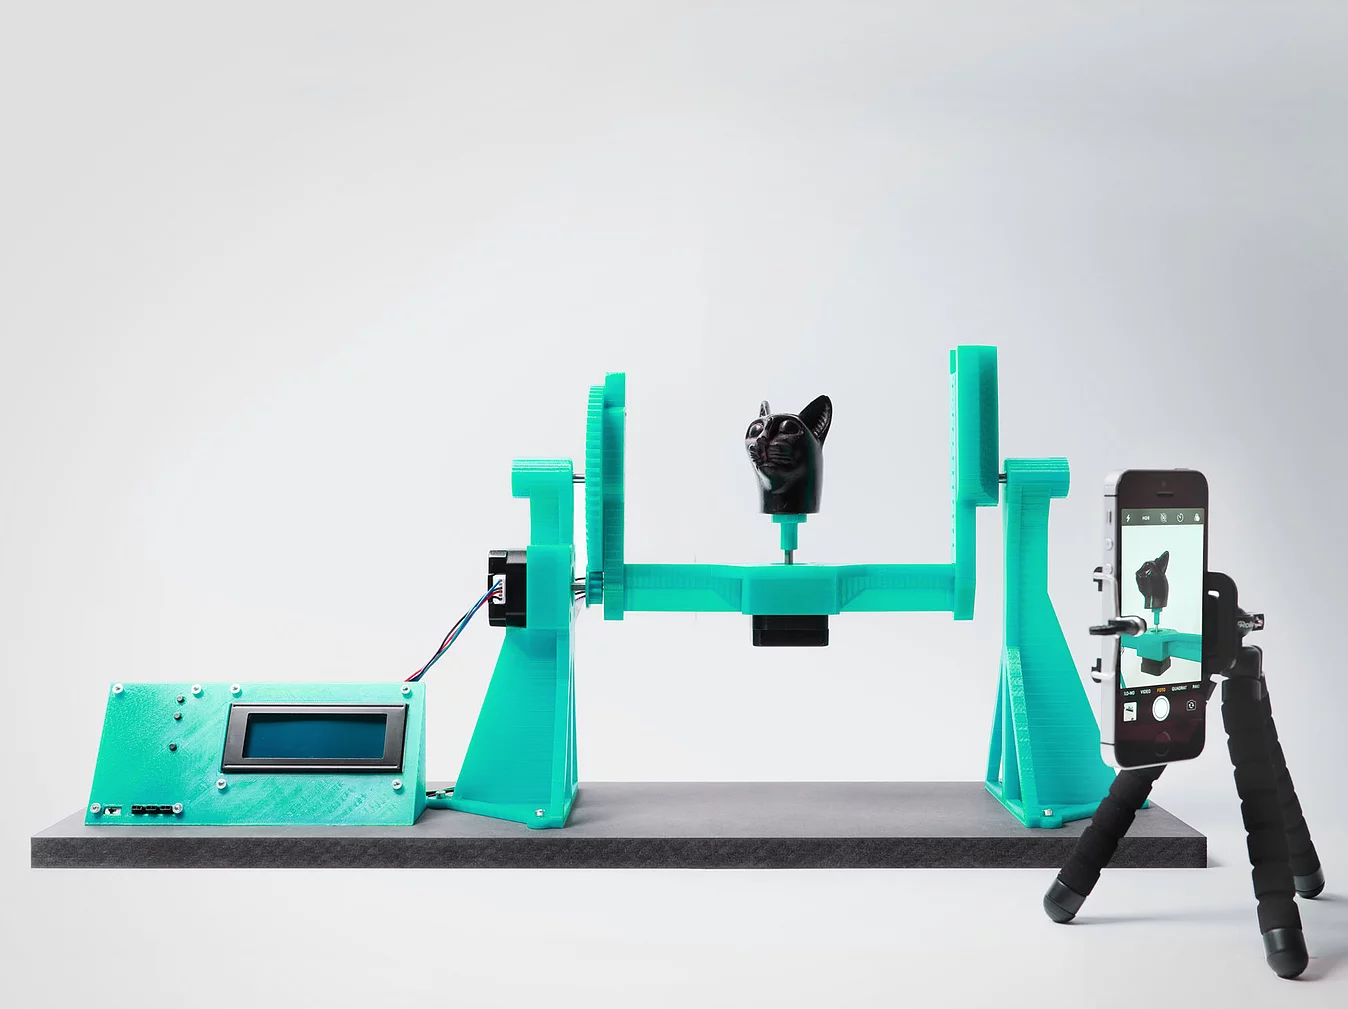
\includegraphics[width=\linewidth]{images/OpenScan.png}\captionof{figure}{The OpenScan 3D Scanner}}%

OpenScan is based on automatically rotating the object to be scanned on two axes (X and Z) while automatically shooting the photos.%

The OpenScan project, like the Open3DScanner, relies on existing cameras that are connected to the scanner. One possibility that OpenScan offers, but was omitted from the Open3DScanner, is the usage of various SLR cameras for 3D scanning. The SLR camera is connected to the scanner via an infrared remote shutter which is connected to the scanner via an optocoupler. This option was removed for the Open3DScanner, because I don't own a SLR camera, nor do I plan to buy one. Furthermore, I am convinced that the quality of modern smartphone cameras is sufficient for the production of good quality 3D scans.%

A feature of the Open3DScanner that OpenScan does not provide is the possibility to connect LED lights directly to the 3D scanner and let the hardware control them during the scanning process.%

While there is no information about the applicable license on the project's homepage, the \hrefIdx{https://www.thingiverse.com/thing:3050437}{OpenScan Thingiverse project} indicates that the project is published under the CC-BY-NC 3.0 license.%

Scans with the OpenScan 3D Scanner are performed fully automatically after the settings for the respective scan have been selected. It is possible to configure how many images are taken per rotation of the z-axis and by which angle the scanner should rotate on the x-axis. In addition, it is possible to determine at how many positions on the x-axis a stop should be made, which in turn results in a complete rotation of the z-axis.%

In addition, there is a setting to adjust the time the scanner stops for each photo. This is important to ensure that the camera can refocus if necessary and avoid blurry shots.%

\infoInfo{Note}{Although the Open3DScanner was developed on the basis of the OpenScan project, it is not a simple copy. After OpenScan motivated the development of the Open3DScanner, requirements were defined independently from the original project. All artifacts (3D models, firmware, BOM) were developed especially for the Open3DScanner.}%

\section{3D Scanner Turntable}%
\label{s:3dTurn}%
Another open source photogrammetry 3D scanner is the project 3D Scanner Turntable by Dave Clarke.%

\hrefIdx{https://www.hackster.io/daveclarke/3d-scanner-turntable-for-cell-phones-updated-64fdb8}{3D Scanner Turntable}%
\marginElement{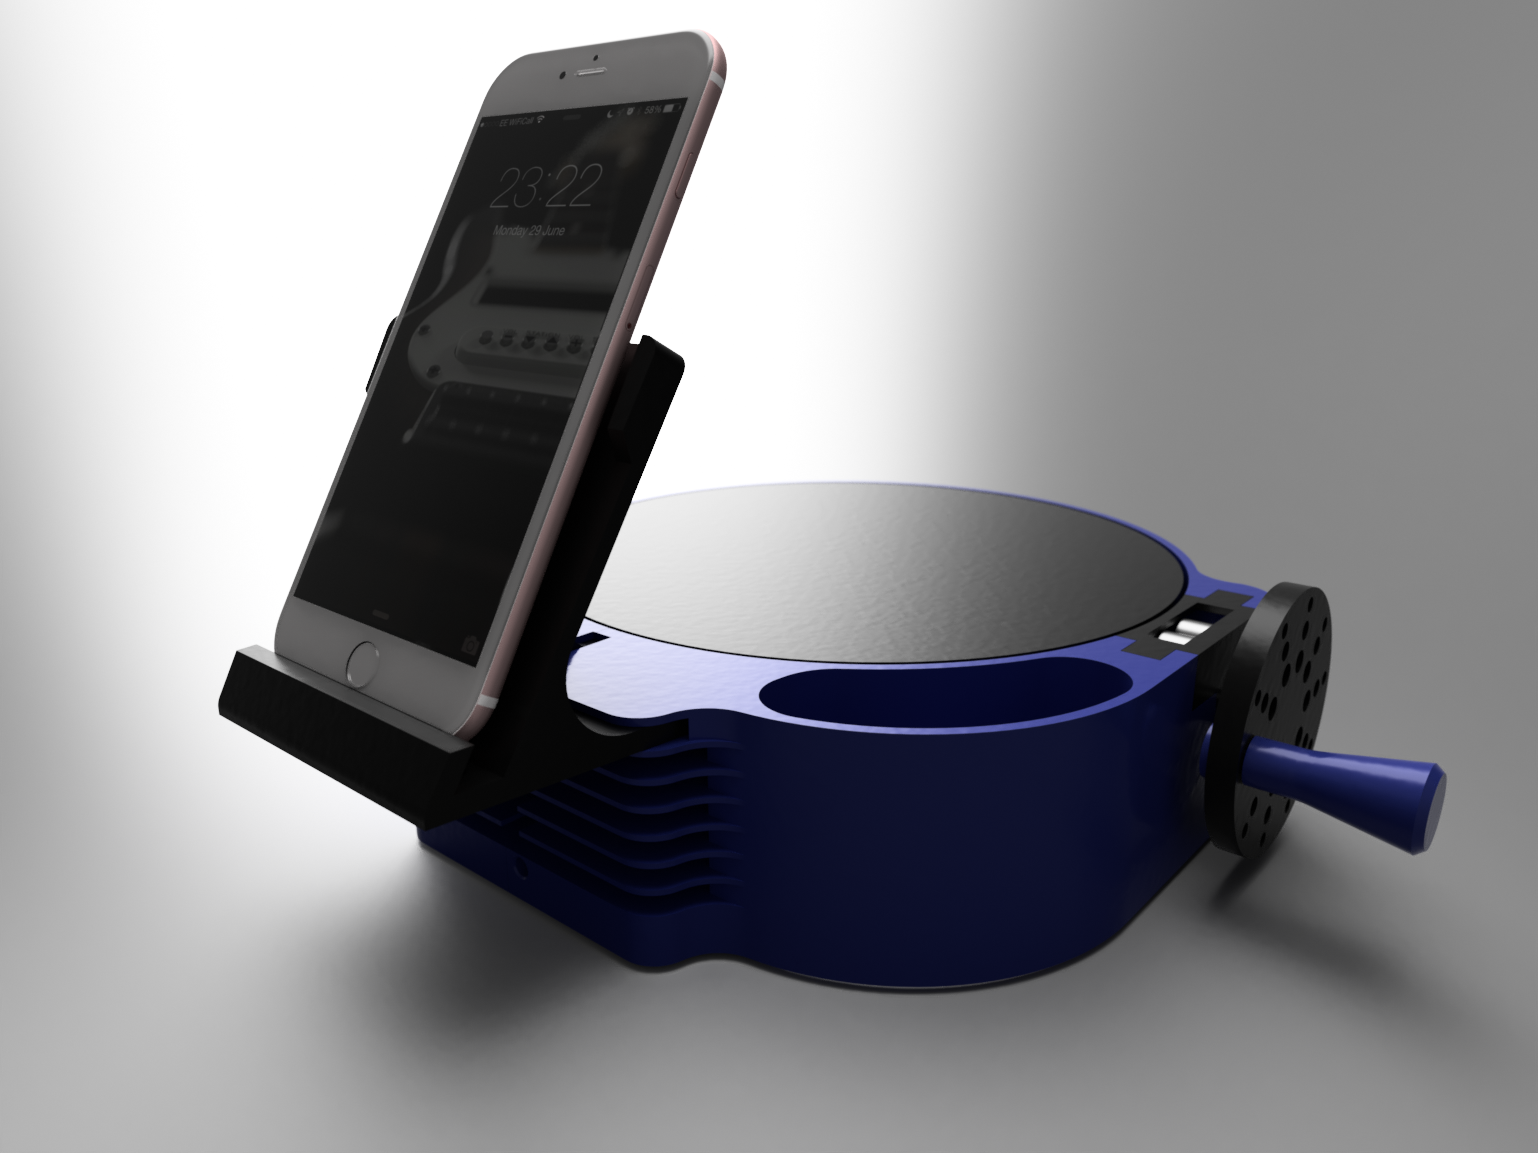
\includegraphics[width=\linewidth]{images/3DTurntable.png}\captionof{figure}{The 3D Scanner Turntable}}

It relies on the use of a smartphone camera and promises that only the filament costs (\SI[round-precision=2,round-mode=places,round-integer-to-decimal]{30}[\$]) will be incurred for the construction of the 3D scanner. In addition to the smartphone, matching headphones with buttons that allow the camera to be released are required.%

In order to achieve the goal of a 3D scanner that is as inexpensive as possible, the project does not use additional electronics that automate scanning. Instead, it is necessary for the user to turn a crank that rotates the object to be scanned and ensures that the smartphone takes 55 photos every full turn.%

Unlike the Open3DScanner or the OpenScan, the object is only rotated on one axis during the scan, so it may be necessary to perform several scans and reposition the object each time. It is therefore necessary for the user to interact more strongly with the 3D scanner during use, but this is the only way to keep costs so low compared to other projects.%

As with the OpenScan project, the captured images must then be processed with appropriate software in order to obtain a 3D model.%

\section{Ciclop}%
The Ciclop 3D Scanner is an ambitious project of Jesús Arroyo, published by bq and based on laser triangulation. In addition to the 3D scanner itself, the project also provides its own software (Windows, Linux, and Mac OS X) for performing the 3D scans.%

\hrefIdx{http://diwo.bq.com/en/einfuhrung-ciclop-und-horus/}{Ciclop}%
\marginElement{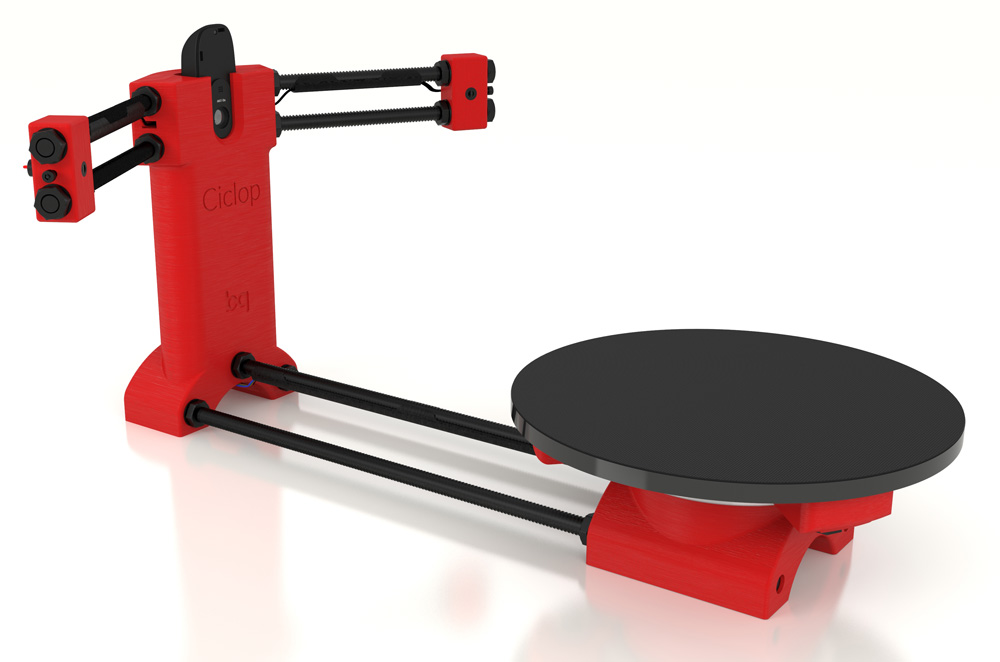
\includegraphics[width=\linewidth]{images/Ciclop.jpg}\captionof{figure}{The Ciclop 3D Scanner}}%

Even though this project has no influence on the development of the Open3DScanner, it shall be introduced briefly here, as it is a wonderful open source hardware project for the creation of a 3D scanner, which provides detailed source information and documentation.%

The result of a scan is a point cloud, which has to be converted into a 3D model with other software (e.g. \hrefIdx{https://www.blender.org/}{Blender}) before the model can be used further, e.g. for 3D printing.%

The whole project is published under the CC-BY-SA 3.0 license as well as the GPL v2.%

Unlike the previous projects, the Ciclop is not based on external hardware (like the camera of a smartphone), but is a complete project in itself, requiring only a PC for operation.%

The core of the project is formed by a \hrefIdx{https://www.logitech.com/en-us/product/hd-webcam-c270}{Logitech C270 HD webcam} for creating the photos and two class 1 lasers, which are used to sample the object. The object to be scanned is positioned on a plate which is automatically rotated.%
	\chapter[Used Software, Tools, etc.]{Used Software, Tools, etc.}%
\label{c:usedSoftware}%
This chapter provides an overview of the software and tools used to implement the Open3DScanner project. Furthermore used artefacts (libraries, 3D models, \dots) as well as the corresponding licenses are presented.%

The aim is to create an as complete as possible list of the dependencies of the Open3DScanner in order to have all relevant license information at one central location.%

Transitive dependencies, which result from the used artefacts, are excluded from the consideration. If you are interested, please refer to the documentation of the respective artifact, which is linked at the appropriate place of this document, if available.%

\section{Arduino}%
Since the heart of the Open3DScanner is an ESP32\sideNote[white]{Detailed information about the ESP32, including its data sheet, can be found on the \hrefIdx{https://www.espressif.com/en/products/hardware/esp32/overview}{Espressif ESP32 product page}.} and the development should be done with the \hrefIdx{https://www.arduino.cc/en/main/software}{Arduino IDE}, one of the most important dependencies in the Arduino area is the {\faGithub} \hrefIdx{https://github.com/espressif/arduino-esp32}{Arduino core for ESP32 WiFi chip}, which allows the use of ESP32 development boards with the Arduino IDE. This simplifies the development of the project considerably.%

The Arduino IDE is released under the GPL license, while the included libraries are released under the LGPL license. The LGPL license is also applied to the Arduino core for the ESP32 WiFi chip.%

\subsection{Libraries}%
In the following the libraries which were used for the implementation of the Open3DScanner and are not included in the Arduino IDE are described.%

\begin{table}[ht!]%
	\begin{centered}%
		\rowcolors{2}{tableLineTwo}{tableLineOne}% specify rowcolors in tabularx style
		\begin{tabularx} {\linewidth} {>{\rowmac \hsize=1.3\hsize}X>{\rowmac \hsize=0.5\hsize}X>{\rowmac \hsize=0.9\hsize}X>{\rowmac \hsize=0.8\hsize}X>{\rowmac \hsize=1.5\hsize}X<{\clearrow}}%
			\tabularxHeader%
			Library & Version & Author & License & Purpose\\%
			{\faGithub} \hrefIdx{https://github.com/platisd/nokia-5110-lcd-library}{nokia-5110-lcd-library} & 2.0.0 & platisd & MIT License & Driving the Nokia 5110 LCD.\\%
			{\faGithub} \hrefIdx{https://github.com/laurb9/StepperDriver}{StepperDriver} & 1.1.4 & laurb9 & not specified & Two-pin stepper motor driver library.\\%
			{\faGithub} \hrefIdx{https://github.com/madhephaestus/ESP32Encoder/}{ESP32Encoder} & 0.1.5 & madhephaestus  & MIT License & Rotary encoder library using interrupts.\\%
			{\faGithub} \hrefIdx{https://github.com/jonblack/arduino-menusystem}{arduino-menusystem} & 3.0.0 & jonblack & MIT License & Ddata structures for menu structures.\\%
		\end{tabularx}%
		\caption{Arduino Libraries used within the Open3DScanner}%
	\end{centered}%
\end{table}%

It can be seen that only a few external libraries are required in total, since a large part of the functionality is already available through the libraries provided by the Arduino IDE and the Arduino core for ESP32 WiFi chip.%

\marginElement{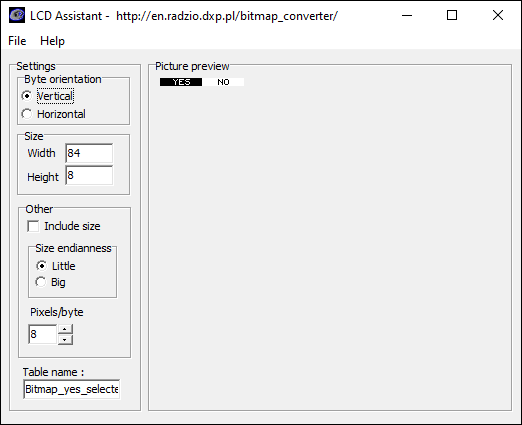
\includegraphics[width=\linewidth]{images/LCDAssistant.png}\captionof{figure}{LCDAssistant GUI}}%

In some places the display of the Open3DScanner shows other things as pure text, e.g. to show buttons. For this purpose, corresponding bitmaps were created, which were then translated into corresponding character arrays with the tool \hrefIdx{http://en.radzio.dxp.pl/bitmap_converter/}{LCD Assistant}\marginInfo[LCDAssistant]{The LCDAssistant is a useful tool that allows the easy transformation of bitmaps into character arrays, which can directly fed to the various LCD screens. It provides some configuration to match different LCDs.} from Radosław Kwiecień.%

The license of the LCD Assistant is not specified by the developer on the project page.%

\section{Schematics and PCB Design}%
Although it is practical to test the necessary circuits on a solderless breadboard during development, this is not a long-term solution. This is especially true if you consider that the breadboard creates new sources of error.%

In addition to the generally known problems, such as instability (in general, but also with e.g. vibrations) and high space requirements compared to a custom PCB, it must be noted that the individual tracks of the breadboard have high resistances and can introduce unwanted capacitances into the circuit\sideNote{More information about unwanted side effects that can occur when using breadboards can be found on \hrefIdx{https://hackaday.com/2016/01/19/solderless-breadboard-parasitics/}{Hackaday} and \hrefIdx{https://breadboardadventures.com/2016/02/14/a-square-and-triangle-wave-vco-part-ii-taming-the-voltage-spikes/}{Breadboard Adventures}.}.%

During development it was not possible to use an LDO\sideNote{Low Dropout} regulator on the breadboard and to get a stable output voltage of \SI{5}{\volt}. Instead it was necessary to outsource the low-dropout and its components to a prototype PCB to get a stable output voltage. Otherwise, it would not have been possible to test the circuit design, as spontaneous voltage drops led to crashes of the ESP32.%

Figure~\ref{f:breadboard} shows the circuit of the Open3DScanner on a breadboard. In addition the prototype PCB with the LDO regulator is visible. It's easy to see that the circuit is chaotic and therefore difficult to maintain, debug, and develop. For the picture even cables have been removed: The stepper motors are not connected and the lights have been removed.%

Due to the size of the components it was necessary to use two breadboards, which makes the whole construction extremely fragile. More than 50 cables were needed to build the circuit on the breadboards.%

\begin{figure}[ht!]%
	\begin{centered}%
		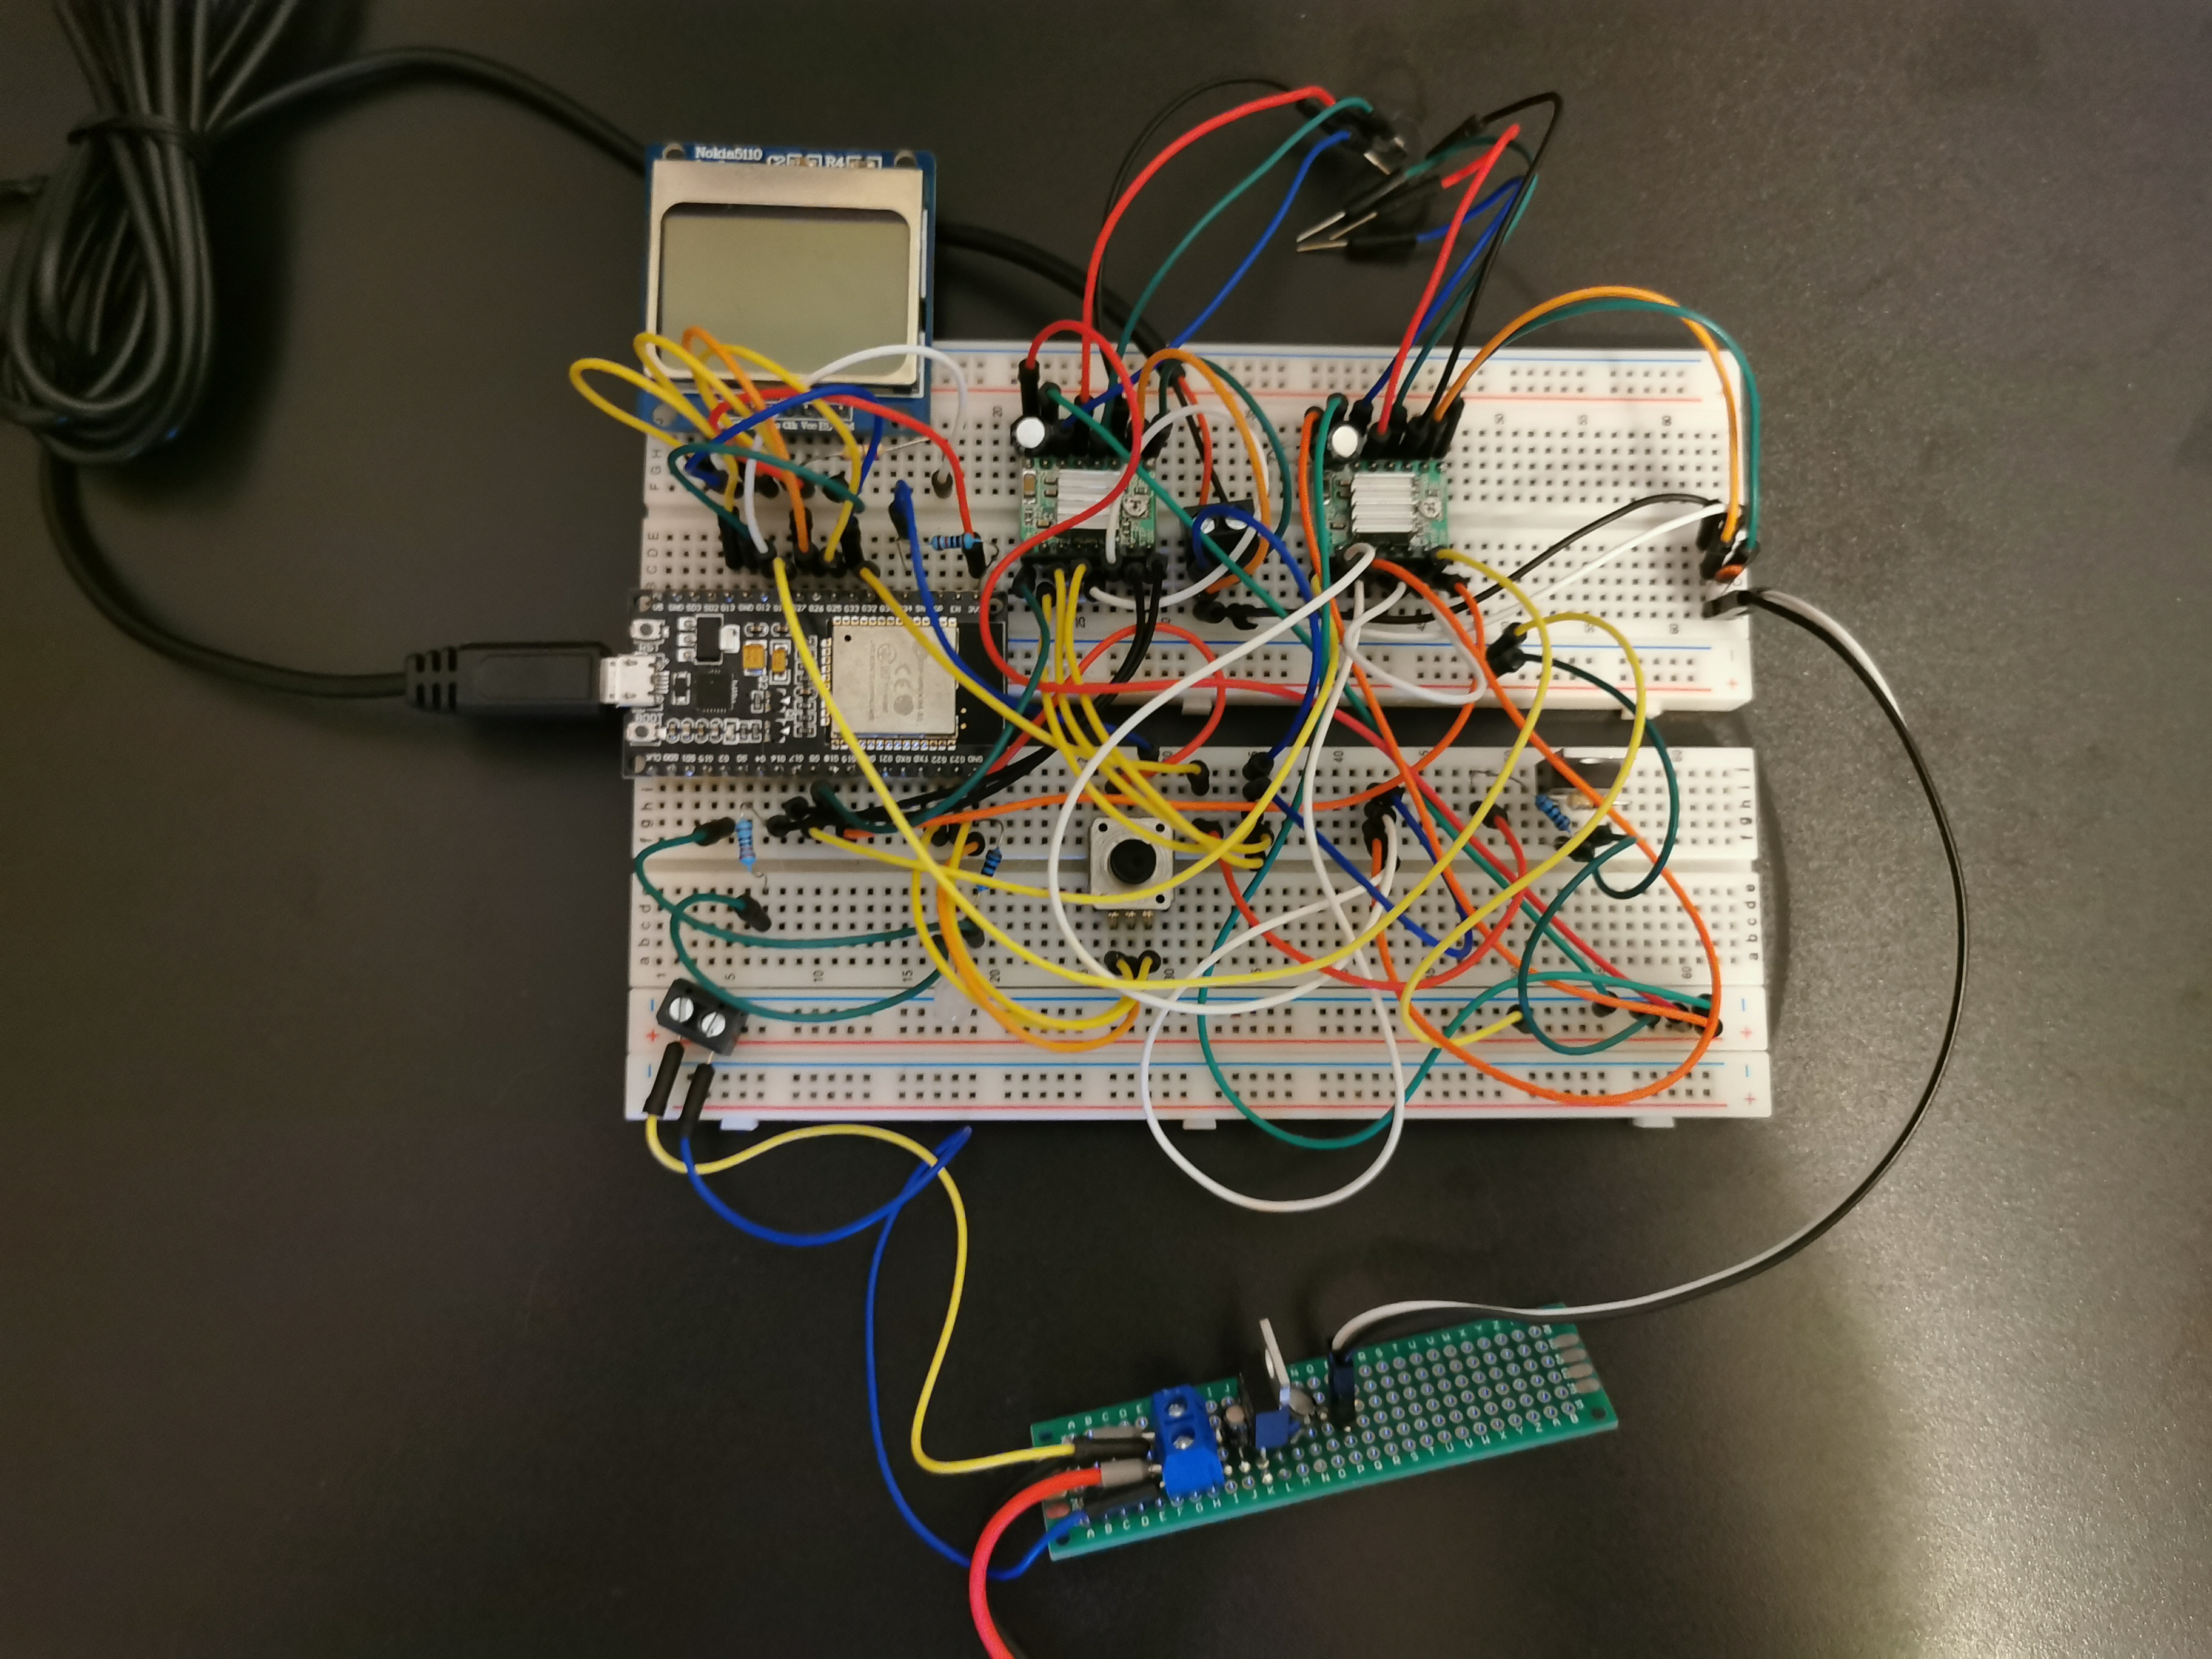
\includegraphics[width=\linewidth]{images/Breadboard.jpg}%
		\caption{The Open3DScanner circuit on a solderless Breadboard}%
		\label{f:breadboard}%
	\end{centered}%
\end{figure}%

It quickly becomes clear that in the long run it is necessary to design and manufacture\marginTips[JLCPCP]{The PCBs for the first prototype of the Open3DScanner were manufactured by \hrefIdx{https://jlcpcb.com/}{JLCPBP}. The manufacturer is located in China and offers very cheap PCBs, which were of very good quality when I ordered them. The only disadvantage, besides the minimum order of 5 boards, is that even the fastest shipping takes about a week. However, this is more than compensated when comparing prices with local suppliers.} a special PCB for the Open3DScanner.%

For the design of the board the software \hrefIdx{http://www.kicad-pcb.org/}{KiCad} was used.  KiCad is an open source program package licensed under the GPL.%

KiCad contains tools for all steps involved in designing a PCB. The individual tools offer very good integration with each other, which simplifies the design process considerably.%

First you create a schematic diagram for the circuit. The individual components are connected with so-called footprints. These footprints define the layout of the individual components on the board (holes, labels, \dots). With this information you go over to the actual design of the PCB. Figure~\ref{f:schematic} shows the schematic diagram for the Open3DScanner.%

\begin{figure}[ht!]%
		\sideCaptionOfL{figure}{Schematic diagram for the Open3DScanner designed in KiCad}{f:schematic}%
		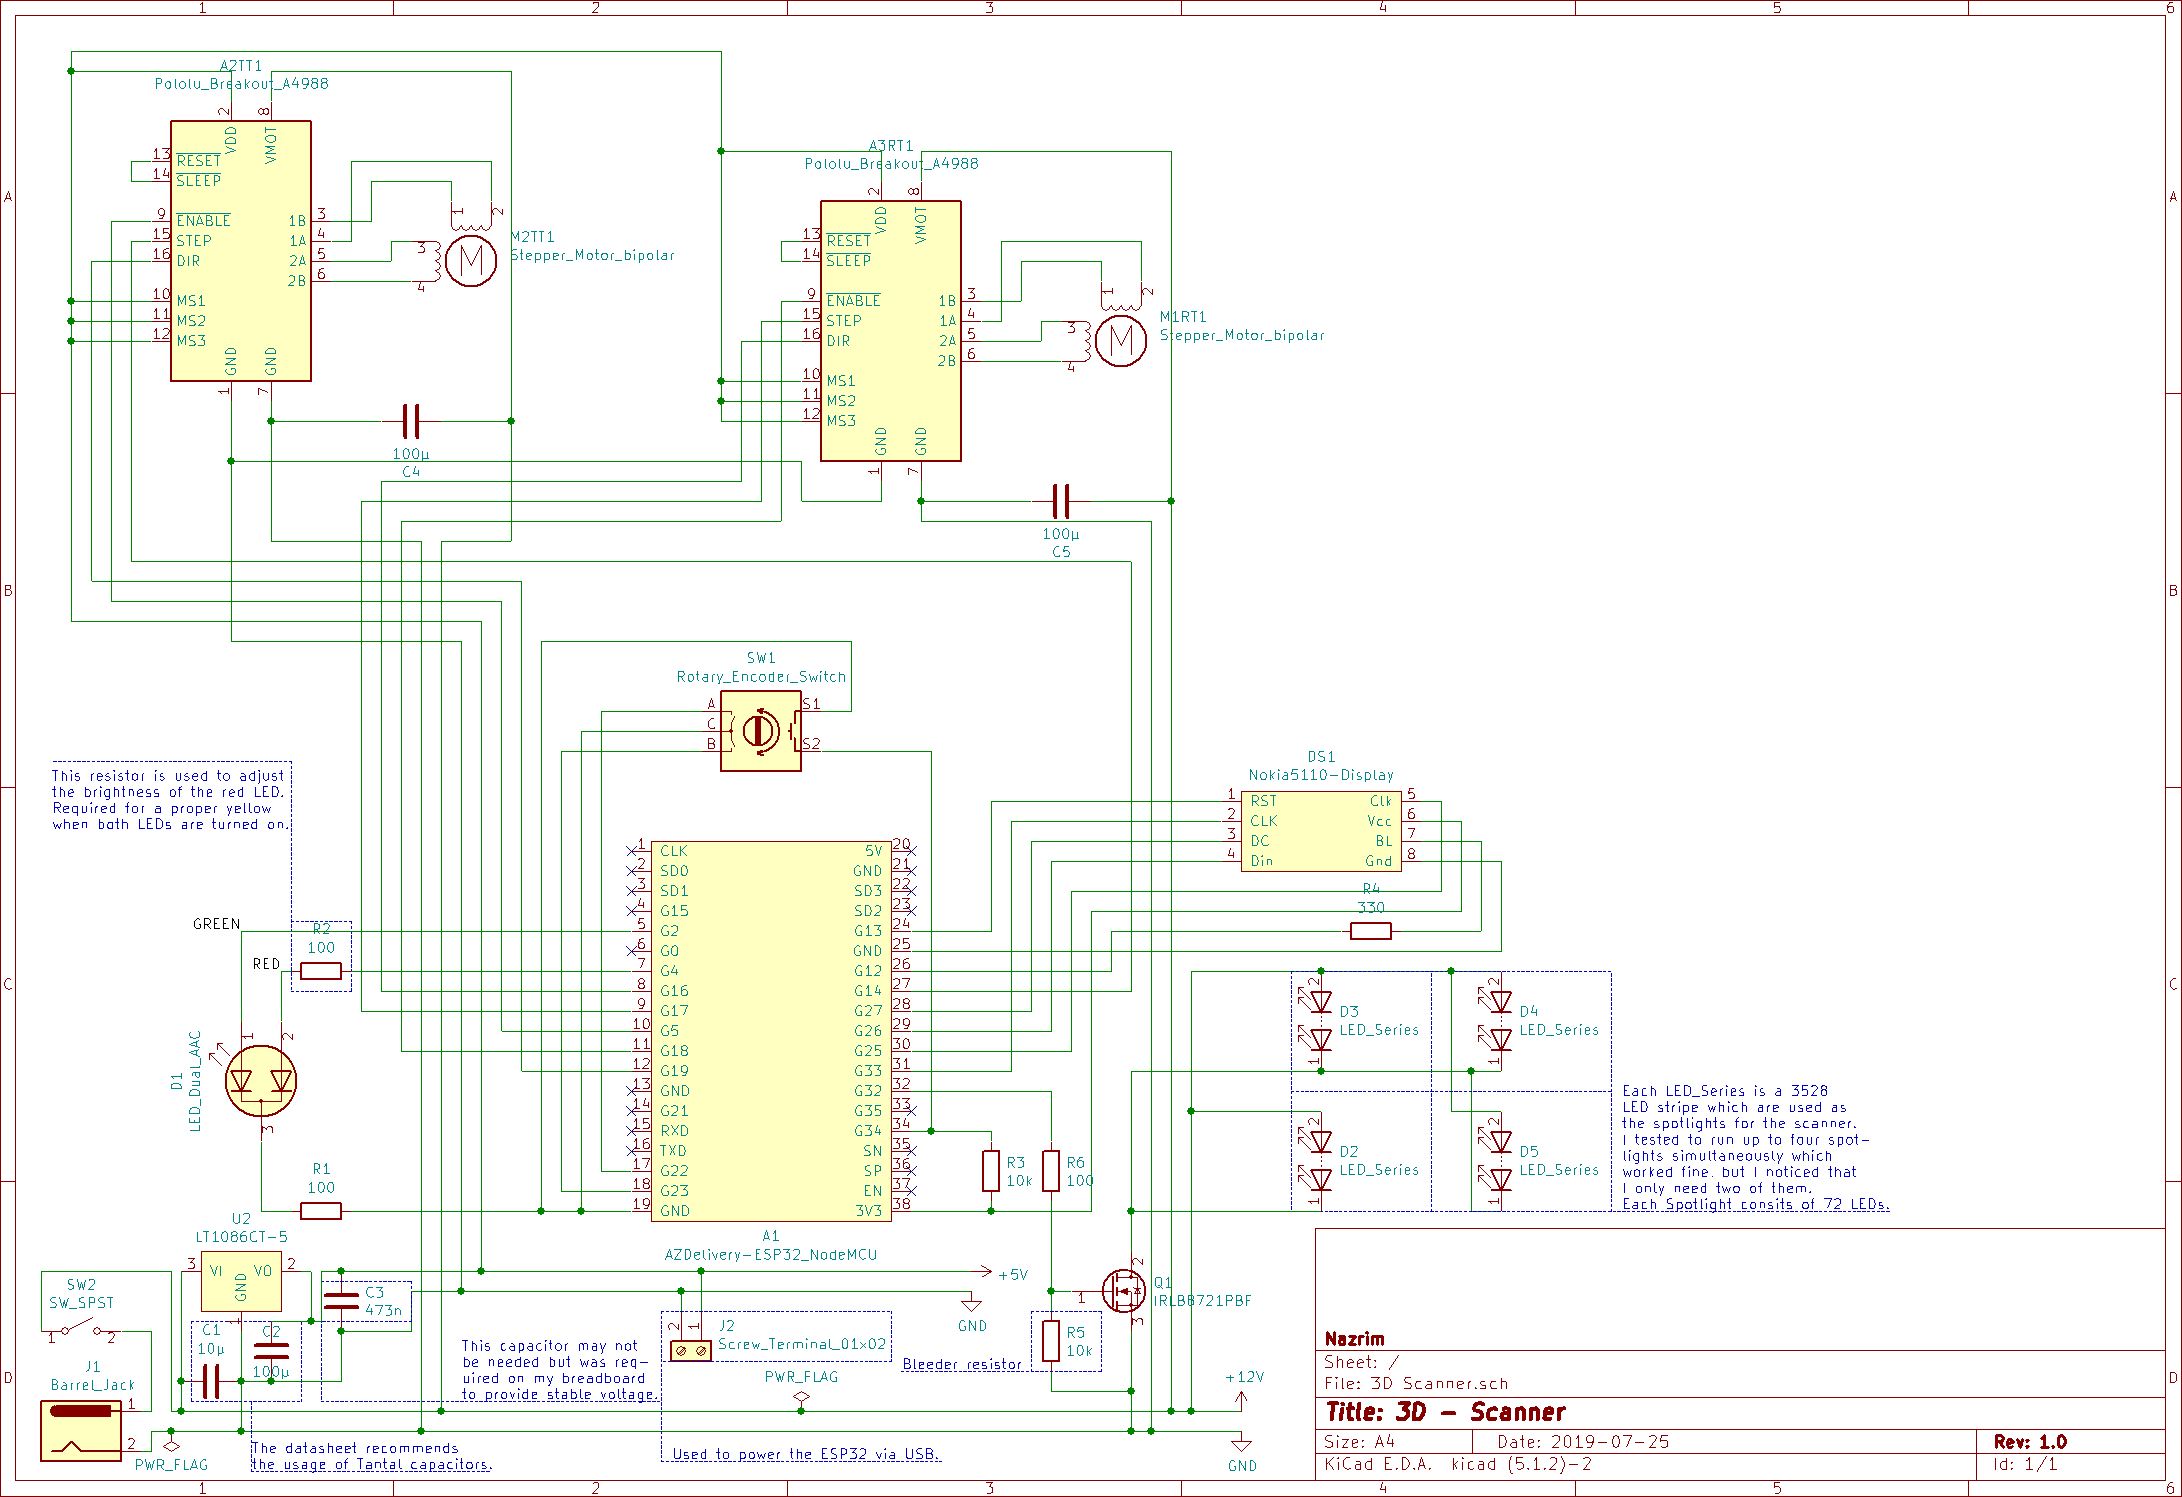
\includegraphics[width=\linewidth]{images/Schematic.png}%
\end{figure}%


All elements are placed on an empty surface, which represents the later board. The user now has to position the individual elements and draw traces for the connections. The user is always shown which pins have to be connected to each other. Figure~\ref{f:pcb} shows the PCB design for the Open3DScanner.%

\begin{figure}[ht!]%
		\sideCaptionOfL{figure}{PCB design for the Open3DScanner designed in KiCad}{f:pcb}%
		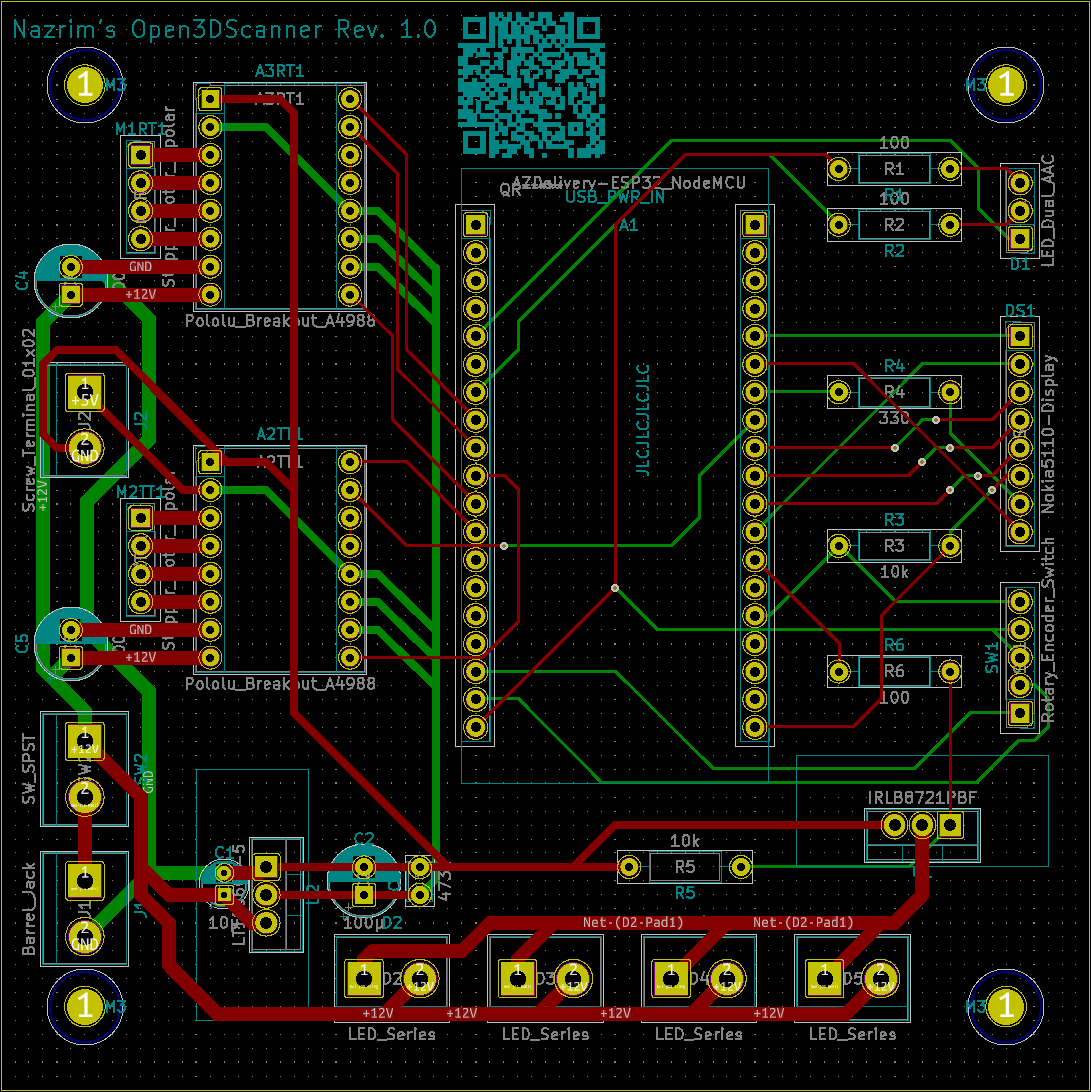
\includegraphics[width=\linewidth]{images/PCB.png}%
\end{figure}%

At this point all necessary steps for the design of the PCB are completed. The necessary Gerber files\marginInfo[Gerber Files]{Manufacturers generally provide instructions on which Gerber files to use and which naming conventions to follow. Often there are even instructions for concrete software.} can be generated and handed over to an appropriate service provider for production.%

Alternatively, a 3D model of the finished board (with all components) can be created beforehand. For this it is necessary to link the footprints with 3D models. For the rendering of the 3D model no further effort is necessary.%

I consider this step very useful. On the one hand you get a better idea of what the finished board will look like and on the other hand you can check again that no components are in conflict with each other. This is especially important in case of a high packing density of the components. Figure~\ref{f:render} shows the rendered 3D model of the Open3DScanner's board including all components.%

\begin{figure}[ht!]%
	\sideCaptionOfL{figure}{3D rendering of the PCB including components for the Open3DScanner designed in KiCad}{f:render}%
	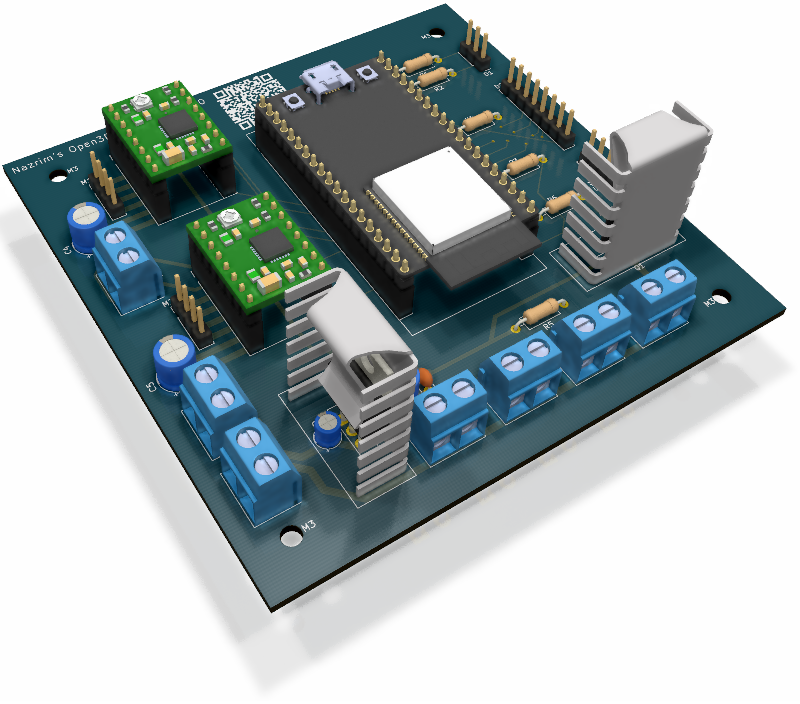
\includegraphics[width=\linewidth]{images/Render.png}%
\end{figure}%

Due to the large number of existing components, KiCad cannot contain a schematic symbol, footprint, and 3D model for all of them. It is also possible that a different footprint should be selected for a component, for example because it is not connected directly to the board, but via a pin header.%

This also applied to several parts of the Open3DScanner. In case of missing schematic symbols and footprints, it is possible to draw the corresponding parts via intuitive integrated editors.%

If 3D models for components are missing, it is necessary to provide them (for example as STEP file). If this does not happen, the board can still be rendered, but the corresponding part locations remain empty.%

A possible source for corresponding 3D models of components to be used in open source projects is  \hrefIdx{https://grabcad.com/library}{GrabCAD}\marginCritical[GrabCAD License]{3D models obtained from GrabCAD may only be used for non-commercial purposes. For commercial use, permission must be obtained from the author of the model.}. For licensing reasons I prefer other sources for obtaining 3D models of components. On the one hand many manufacturers already provide corresponding CAD files and on the other hand \hrefIdx{https://www.snapeda.com/}{SnapEDA} offers a large database of components containing a schematic symbol, a PCB footprint, and a 3D model. The individual entries are licensed under CC-BY-SA 4.0.%

\subsection{Used 3D Models}%
This section lists the 3D models which are not already part of KiCad and which are used to render the Open3DScanner board and their source.%

\begin{table}[ht!]%
		\sideCaptionOf{table}{3D Models used for rendering the Open3DScanner}%
		\rowcolors{2}{tableLineTwo}{tableLineOne}% specify rowcolors in tabularx style
		\begin{tabularx} {\linewidth} {>{\rowmac \hsize=\hsize}X>{\rowmac \hsize=\hsize}X<{\clearrow}}%
			\tabularxHeader%
			Component & Source\\%
			ESP32 Devkit-C  & \href{https://www.snapeda.com/parts/ESP32-DEVKITC-32D/Espressif\%20Systems/view-part/}{SnapEDA - ESP32-DEVKITC-32D}\\%
			Blue two pole screw terminal & \hrefIdx{https://www.snapeda.com/parts/TB002-500-02BE/CUI\%20Inc./view-part/}{SnapEDA - TB002-500-02BE}\\%
			A4988 stepper driver & \hrefIdx{https://www.pololu.com/product/1182}{Pololu - A4988 product page}\\%
			TO 220 attachable heatsink & \hrefIdx{https://www.fischerelektronik.de/web\_fischer/en\_GB/heatsinks/C02/Attachable\%20heatsink/PG/FK245MI247O/search.xhtml}{fischer elektronik - FK 245 MI 247 O product page}\\%
		\end{tabularx}%
\end{table}%

\section{3D Design}%
When it comes to the 3D modeling of the Open3DScanner, there is little special to mention.%

\marginElement{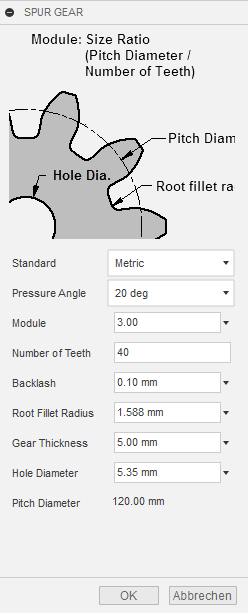
\includegraphics[width=\linewidth]{images/Spur_gear_3d_scanner_gear.png}\captionof{figure}{Fusion 360 script settings for creating the Open3DScanner's spur gear}}%

All components needed for the project and printed with a 3D printer were designed with \hrefIdx{https://www.autodesk.de/products/fusion-360/overview}{Fusion 360}. It should be noted that Fusion 360 contains handy scripts to create certain elements automatically. One of these scripts allows the creation of gears with given parameters. This script was used for the gears in the Open3DScanner.%

CAD models of some standard components such as ball bearings are required for the subsequent building instructions and render images of the finished Open3DScanner.%

\begin{table}[ht!]%
	\rowcolors{2}{tableLineTwo}{tableLineOne}% specify rowcolors in tabularx style
	\begin{tabularx} {\linewidth} {>{\rowmac \hsize=1.2\hsize}X>{\rowmac \hsize=0.9\hsize}X>{\rowmac \hsize=0.9\hsize}X<{\clearrow}}%
		\tabularxHeader%
		Source & Model Type & License\\%
		\hrefIdx{https://www.astbearings.com/free-3d-cad-models-for-bearings.html}{AST Bearings} & Bearings & not specified, but free\\%
		\faGithub{} \hrefIdx{https://github.com/Hecatron-Machines/Cad.Solidworks.Parts}{Cad.Solidworks.Parts}& Nema 17 & MIT\\%
		\hrefIdx{https://octopart.com/terms}{Octopart} & Various & not specified, but free\\%
		\faGithub{} \hrefIdx{https://github.com/FreeCAD/FreeCAD-library}{FreeCAD-library}& Dupont Connectors & CC-BY 3.0\\%
		\hrefIdx{https://www.digikey.de//resources/3d-models}{Digi-Key}& Molex Connectors \& Cable Lugs & not specified, but free\\%
		\hrefIdx{https://www.snapeda.com/}{SnapEDA}& Micro USB-B Connector & CC-BY-SA 4.0\\%
	\end{tabularx}%
	\caption{Sources for CAD models of non-electrical components}%
	\label{t:cad}%
\end{table}%

There are several vendors with large libraries of CAD models, which may not be freely used and/or distributed. Table~\ref{t:cad} contains information which offers were used for which models.%

\section{Photogrammetry}%
\label{sec:photogrammetry}
The heart of the entire photogrammetry process is the software that creates the 3D model from the images taken.%

For this purpose I use the software \hrefIdx{https://alicevision.org/\#meshroom}{Meshroom}. It is intuitive to use and performs the entire process. The finished (textured) 3D model is created from the fed-in images. Alternative software solutions do not always offer the entire process and generate for example only a point cloud, which has to be converted into a 3D model with another program. This applies for example to \hrefIdx{http://ccwu.me/vsfm/}{VisualSFM}.%

Meshroom is released under the MPL 2.0 and can be compiled by the user or can be obtained as a ready-to-use installer.%

In general, I would recommend the use of Meshroom to anyone, simply because it is very easy to use and produces great results while offering extensive configuration options.%

The only limitation is that a CUDA-enabled graphics card (Nvidia) is required for optimal results, as the calculations are done on the GPU. If such a card is not available, a "preview mode" can be activated, which works without CUDA, but also produces worse results.%

\section{\LaTeX}%
\LaTeX{} was used to create this manual and last but not least we will look at which packages were used to create it.%

The document class used is yReport from Harvey Sheppard. The class is part of his project {\faGithub} \hrefIdx{https://github.com/HarveySheppard/yLaTeX}{yLatex}, which provides document classes and packages to create appealing documents. The entire yLatex project is licensed with LPPL 1.3.%

The compiler used is \hrefIdx{http://www.tug.org/xetex/}{\hologo{XeLaTeX}}, which is required by the document class yReport. \hrefIdx{https://www.tug.org/texlive/}{\hologo{TeX} Live} is used as \hologo{TeX} distribution and \hrefIdx{https://www.texstudio.org/}{\hologo{TeX}studio} as editor.%

Pictures can be found in various places in this document. If these images are not photos, screenshots, or exports from other software, the images were created with Gimp which is licensed under the GPL.%

In addition, various packages are used to realize individual aspects of the document. These are listed below.%

\begin{table}[ht!]%
	\begin{centered}%
		\rowcolors{2}{tableLineTwo}{tableLineOne}% specify rowcolors in tabularx style
		\begin{tabularx} {\linewidth} {>{\rowmac \hsize=1.0\hsize}X>{\rowmac \hsize=0.7\hsize}X>{\rowmac \hsize=1.0\hsize}X>{\rowmac \hsize=0.5\hsize}X>{\rowmac \hsize=1.8\hsize}X<{\clearrow}}%
			\tabularxHeader%
			Package & Version & Maintainer & License & Purpose\\%
			\hrefIdx{https://ctan.org/pkg/fontawesome}{fontawesome5}  & 5.9.0 & Marcel Krüger & LPPL 1.3c \& OFL & Required by yAuthorBlock and used to show some icons across the document.\\%
			{\faGithub} \hrefIdx{https://github.com/HarveySheppard/yLaTeX}{yAuthorBlock}  & unknown & Harvey Sheppard & LPPL 1.3 & Used to create the author block on the second page.\\%
			\hrefIdx{https://ctan.org/pkg/tabularx}{tabularx}  & 2.11 & The \LaTeX{} Team & LPPL 1.3 & Since tabu (used by yReport) is somewhat buggy, this document uses tabularx.\\%
			\hrefIdx{https://ctan.org/pkg/siunitx}{siunitx}  & 2.7s & Joseph Wright & LPPL 1.3c & Used to display numbers and units in a proper way.\\%
			\hrefIdx{https://ctan.org/pkg/indextools}{indextools}  & 1.5.1 & Maïeul Rouquette & LPPL 1.3 & Used to build an index of all weblinks for printed documents.\\%
			\hrefIdx{https://ctan.org/pkg/xparse}{xparse} & 2019-05-28 & The \LaTeX{} Team & LPPL 1.3c & Required for string magic to display urls in the index (Appendix~\ref{ca:refs}) in a proper way.\\%
			{\faGithub} \hrefIdx{https://github.com/HarveySheppard/yLaTeX}{infoBulle}  & unknown & Harvey Sheppard & LPPL 1.3 & Used for displaying various block types (info, warning, \dots) in main area.\\%
			{\faGithub} \hrefIdx{https://github.com/HarveySheppard/yLaTeX}{marginInfoBulle}  & unknown & Harvey Sheppard & LPPL 1.3 & Used for displaying various block types (info, warning, \dots) in margin area.\\%
			\hrefIdx{https://ctan.org/pkg/isodate}{isodate}  & 2.28 & Harald Harders & LPPL 1.3c & Used for uniform displaying dates. Required because of strange behaviour of datetime package (included in yReport).\\%
			\hrefIdx{https://ctan.org/pkg/xurl}{xurl}  & 0.07 & Herbert Vo\ss{} & LPPL 1.3 & Allow URL breaks at any alphanumerical character.\\%
			\hrefIdx{https://ctan.org/pkg/hologo}{hologo}  & 1.13 & Heiko Oberdiek & LPPL 1.3 & Used to disaplay logos from the \LaTeX{} family.\\%
		\end{tabularx}%
		\caption{Used \LaTeX{} packages within the Open3DScanner's manual}%
	\end{centered}%
\end{table}%
%
	\chapter{Required Parts}%
\label{c:bom}%
This chapter shows which things are needed to build the Open3DScanner. It looks at the components of the printer as well as the tools and devices needed to assemble it.%

It is recommended to read this chapter carefully if you want to build your own Open3DScanner.%

\section{Bill of Materials}%
One of the most important points to build your own Open3DScanner is a bill of materials of the required parts.%

This is contained in the following sections. The complete list is divided into two partial lists. The first one contains all electrical components which can be found on the PCB or are connected to it. The second list contains all further things that are needed to assemble the Open3DScanner.%

\subsection{Electrical Components}%
The following table contains all electrical components required to build the Open3DScanner.%

In addition to the component and the required quantity, the identifier of the respective component on the circuit board is also specified. In addition to this, information is given for individual components, which must be considered when purchasing.%

\begin{table}[ht!]%
	\begin{centered}%
		\rowcolors{2}{tableLineTwo}{tableLineOne}% specify rowcolors in tabularx style
		\begin{tabularx} {\linewidth} {>{\rowmac \hsize=1.4\hsize}X>{\rowmac \hsize=0.3\hsize}X>{\rowmac \hsize=0.6\hsize}X>{\rowmac \hsize=1.7\hsize}X<{\clearrow}}%
			\tabularxHeader%
			Component & Quantity & PCB-Identifier  & Note\\%
			\hrefIdx{https://www.espressif.com/en/products/hardware/esp32-devkitc/overview}{ESP32-DevKitC} & 1 & A1 & While I use the \hrefIdx{https://www.az-delivery.de/products/esp32-developmentboard}{AZ-Delivery ESP32-DevKitC}, any version that meets the \hrefIdx{https://www.espressif.com/en/products/hardware/esp32-devkitc/overview}{ESP32-DevKitC} specification should work.\\%
			\hrefIdx{https://www.pololu.com/product/1182}{A4988 Stepper Driver} & 2 & A2TT1 \& A3RT1 & Any A4988 steper driver should work. I recommend getting matching heat sinks.\\%
			\hrefIdx{https://reprap.org/wiki/NEMA\_17\_Stepper\_motor}{Nema 17 Stepper Motor} & 2 & M1RT1 \& M2TT1 & Make sure to buy the version with D-shaft. I use strong stepper motors, like this \hrefIdx{https://www.omc-stepperonline.com/nema-17-stepper-motor/nema-17-bipolar-59ncm-84oz-in-2a-42x48mm-4-wires-w-1m-cable-and-connector-full-d-cut-shaft.html}{\SI{59}{\newton\centi\meter} Nema 17 stepper motor}.\\%
			\hrefIdx{https://www.analog.com/en/products/lt1086.html}{LT1086CT-5} & 1 & U2 & Ensure to get the \hrefIdx{https://www.centralsemi.com/PDFS/CASE/TO\_220\_PD.PDF}{TO-220} type.\\%
			\hrefIdx{https://www.infineon.com/cms/en/product/power/mosfet/12v-300v-n-channel-power-mosfet/irlb8721/}{IRLB 8721} & 1 & Q1 & Ensure to get the \hrefIdx{https://www.centralsemi.com/PDFS/CASE/TO\_220\_PD.PDF}{TO-220} type.\\%
			TO-220 Heatsink & 2 & Q1 \& U2 & I highly recommend at least one for the \hrefIdx{https://www.analog.com/en/products/lt1086.html}{LT1086CT-5} since it gets very hot during operation. The one for the \hrefIdx{https://www.infineon.com/cms/en/product/power/mosfet/12v-300v-n-channel-power-mosfet/irlb8721/}{IRLB 8721} is just to be safe. While I am using the \hrefIdx{https://www.fischerelektronik.de/web\_fischer/en\_GB/heatsinks/C02/Attachable\%20heatsink/PG/FK245MI247O/search.xhtml}{FK 245 MI 247 O} you can choose whatever fits in the space (about \SI{22.5}{\milli\meter}$\times$\SI{10}{\milli\meter}).\\%
			\SI{1}{\milli\litre} Thermal Paste & 1 & - & Required for a good connection between \hrefIdx{https://www.centralsemi.com/PDFS/CASE/TO\_220\_PD.PDF}{TO-220} components and their heatsink. Only a tiny amount is required.\\%
			\hrefIdx{https://www.alps.com/prod/info/E/HTML/Encoder/Incremental/EC12E/EC12E\_list.html}{STEC12E08 Rotary Encoder} & 1 & - & This will be connected to the pin header SW1.\\%
			\hrefIdx{https://www.sparkfun.com/products/10168}{Nokia 5110 Display} & 1 & - & This will be connected to the pin header DS1. Buy one with screw holes. Hole distance on x-axis should be \SI{34}{\milli\meter} and \SI{40.5}{\milli\meter} on the y-axis.\\%
			\SI{5}{\milli\meter} 3-Pin Bi-Color LED & 1 & - & This will be connected to the pin header D1. I recommend using a red-green one.\\%
			\SI{5}{\meter}$\times$\SI{8}{\milli\meter} 300 LED 3528 Strip, \SI{12}{\volt} \SI{1.5}{\ampere} & 1 & - & This will be connected to the pin headers D2, D3, D4, D5.\\%
			Round \SI{20}{\milli\meter} SPST Rocker Switch (R13 112) & 1 & - & This will be connected to the pin header SW2.\\%
			\SI{5.5}{\milli\meter}$\times$\SI{2.1}{\milli\meter} Female DC Power Jack Panel Mount (L722AS) & 1 & - & This will be connected to the pin header SW2. Make sure to grab one with threads and a nut for panel mounting.\\%
			\SI{473}{\nano\farad} Ceramic Capacitor & 1 & C3 & Choose \SI{2.54}{\milli\meter} pin distance and \SI{3.4}{\milli\meter} radius.\\%
			\SI{10}{\micro\farad} Electrolytic Capacitor & 1 & C1 & Choose \SI{2}{\milli\meter} pin distance and \SI{4}{\milli\meter} radius.\\%
			\SI{100}{\micro\farad} Electrolytic Capacitor & 3 & C2, C4, C5 & Choose \SI{2.5}{\milli\meter} pin distance and \SI{6.3}{\milli\meter} radius.\\%
			\SI{100}{\ohm} Resistor & 3 & R1, R2, R6 & Choose whatever you have at hand, like carbon film or metal (oxide) film.\\%
			\SI{330}{\ohm} Resistor & 1 & R4 & Choose whatever you have at hand, like carbon film or metal (oxide) film.\\%
			\SI{10}{\kilo\ohm} Resistor & 2 & R3, R5 & Choose whatever you have at hand, like carbon film or metal (oxide) film.\\%
		\end{tabularx}%
		\caption{BOM for all electrical components of the Open3DScanner --- Part 1/3}%
	\end{centered}%
\end{table}%
\begin{table}[ht!]%
	\begin{centered}%
		\rowcolors{2}{tableLineTwo}{tableLineOne}% specify rowcolors in tabularx style
		\begin{tabularx} {\linewidth} {>{\rowmac \hsize=1.4\hsize}X>{\rowmac \hsize=0.3\hsize}X>{\rowmac \hsize=0.6\hsize}X>{\rowmac \hsize=1.7\hsize}X<{\clearrow}}%
			\tabularxHeader%
			Component & Quantity & PCB-Identifier  & Note\\%
			\hrefIdx{https://www.sparkfun.com/products/8432}{2-Pin Screw Terminals 5mm Pitch} & 7 & J1, J2, SW2, D2, D3, D4, D5 & Take care to get the ones with 5mm pitch.\\%
			\SI{2.54}{\milli\meter} 40-Pin Header & 1 & M1RT1, M2TT2, D1, DS1, SW1 & Will be cut into 1$\times$3, 2$\times$4, 1$\times$5, and 1$\times$8.\\%
			\SI{2.54}{\milli\meter} 40-Pin Socket & 2 & A1, A2TT1, A3RT1 & Will be cut into 2$\times$19 and 4$\times$8. Each cut results in one socket loss.\\%
			1$\times$3 Dupont Housing & 4 & - & Will be used to connect D1 with the bi-color LED on both sides as well as the STEC12E08 rotary encoder on component side.\\%
			1$\times$5 Dupont Housing & 1 & - & Will be used to connect SW1 with the rotary encoder on PCB side.\\%
			1$\times$8 Dupont Housing & 2 & - & Will be used to connect DS1 with the LCD on both sides.\\%
			Female Dupont Terminals & 33 & - & Required for all Dupont housings.\\%
			Molex crimp housing --- Micro-Fit - 1x2-pin, male (430200201) & 4 & - & Required for connecting the lights to the Open3DScanner. Part number \hrefIdx{https://www.molex.com/molex/products/datasheet.jsp?part=active/0430200201\_CRIMP\_HOUSINGS.xml}{Molex 430200201}\\%
			Molex crimp housing --- Micro-Fit - 1x2-pin, female & 4 & - & Required for connecting the lights to the Open3DScanner. Part number \hrefIdx{https://www.molex.com/molex/products/datasheet.jsp?part=active/0430250200\_CRIMP\_HOUSINGS.xml}{Molex 430250200}\\%
			Molex crimp contact --- Micro-Fit, female  & 8 & - & Required for connecting the lights to the Open3DScanner. Part number \hrefIdx{https://www.molex.com/molex/products/datasheet.jsp?part=active/0430300007\_CRIMP\_TERMINALS.xml}{Molex 430300007}\\%
			Molex crimp contact --- Micro-Fit, male  & 8 & - & Required for connecting the lights to the Open3DScanner. Part number \hrefIdx{https://www.molex.com/molex/products/datasheet.jsp?part=active/0430310007\_CRIMP\_TERMINALS.xml}{Molex 430310007}\\%
			Cable Lug & 4 & - & The cable lugs have to match your power jack and your rocker switch. For me it is 2$\times$\SI{2.8}{\milli\meter} (power jack) and 2$\times$\SI{4.8}{\milli\meter} (rocker switch).\\%
			Power Supply \SI{12}{\volt}, \SI{2250}{\milli\ampere} with \SI{5.5}{\milli\meter}$\times$\SI{2.1}{\milli\meter} male Barrel Jack & 1 & - & This will power the whole Open3DScanner\\%
			\SI{15}{\centi\meter} Micro USB-B cable & 1 & - & Used to connect J2 with the ESP32's usb port. Get an already prepared cable if you can, otherwise you need to cut one yourself.\\%
			AWG 18 or \SI{0.75}{\milli\meter\squared} cable & - & - & Used for transmitting power (e.g. from power jack to PCB, within pieces of the LED strip, and towards the LED strip). Since the cables are not exposed to any or only little movement, no special requirements like silicone cables exist. I use simple speaker cable which is sold in rolls of \SI{25}{\meter}. I cannot provide an accurate required quantity for the wires since it depends somewhat on individual wiring.\\%
		\end{tabularx}%
		\caption{BOM for all electrical components of the Open3DScanner --- Part 2/3}%
	\end{centered}%
\end{table}%
\begin{table}[ht!]%
	\begin{centered}%
		\rowcolors{2}{tableLineTwo}{tableLineOne}% specify rowcolors in tabularx style
		\begin{tabularx} {\linewidth} {>{\rowmac \hsize=1.4\hsize}X>{\rowmac \hsize=0.3\hsize}X>{\rowmac \hsize=0.6\hsize}X>{\rowmac \hsize=1.7\hsize}X<{\clearrow}}%
			\tabularxHeader%
			Component & Quantity & PCB-Identifier  & Note\\%
			AWG 24 or \SI{0.2}{\milli\meter\squared} cable & - & - & Used to connect the various components to the PCB. I cannot provide an accurate required quantity for the wires since it depends somewhat on individual wiring.\\%
			PCB & 1 & - & The Gerber files for the PCB of the Open3DScanner are part of this project and can be used to get PCBs from a manufacturer.\\%
		\end{tabularx}%
		\caption{BOM for all electrical components of the Open3DScanner --- Part 3/3}%
	\end{centered}%
\end{table}%

\subsection{Other Components}%
The previous section contains the BOM for all electrical parts of the Open3DScanner.%

In addition, this section contains a BOM for all remaining parts needed to build the Open3DScanner. The separation should help to better bundle the orders with the respective suppliers.%

It should be noted that the quantities specified for the screws indicate maximum quantities. These can be smaller, e.g. if the maximum of four lights are not mounted.%

\begin{table}[ht!]%
	\begin{centered}%
		\rowcolors{2}{tableLineTwo}{tableLineOne}% specify rowcolors in tabularx style
		\begin{tabularx} {\linewidth} {>{\rowmac \hsize=1.2\hsize}X>{\rowmac \hsize=0.3\hsize}X>{\rowmac \hsize=1.5\hsize}X<{\clearrow}}%
			\tabularxHeader%
			Component & Quantity & Note\\%
			\SI{400}{\milli\meter} $\times$ \SI{550}{\milli\meter} $\times$ \SI{16}{\milli\meter} Wooden Board & 1 & This will be used as the base of the whole Open3DScanner\\%
			\SI{500}{\milli\meter} $\times$ \SI{550}{\milli\meter} $\times$ \SI{3}{\milli\meter} PVC Rigid Foam Sheet & 1 & The rear panel of the Open3DScanner.\\%
			\SI{800}{\gram} Roll ABS Filament & 1 & Main color. Other materials like PLA may be fine.\\%
			\SI{800}{\gram} Roll ABS Filament & 1 & Secondary color. Other materials like PLA may be fine.\\%
			\SI{800}{\gram} Roll ABS Filament & 1 & Accent color. Other materials like PLA may be fine.\\%
			Nema 17 Damper & 2 & For decoupling the motors from the Open3DScanner's structure.\\%
			Liquid Glue & 1 & Required for assembling the lights if the M3 tape which is applied to the LED strip does not hold and to glue some nuts in place.\\%
			\SI{5}{\milli\meter} $\times$ \SI{26}{\milli\meter} Steel Rod & 5 & Used to connect and secure various parts.\\%
			625ZZ Bearing & 2 & Used to connect the moving parts to the frame with as little friction as possible.\\%
		\end{tabularx}%
		\caption{BOM for all non-electrical components of the Open3DScanner 1/2}%
	\end{centered}%
\end{table}%

\begin{table}[ht!]%
	\begin{centered}%
		\rowcolors{2}{tableLineTwo}{tableLineOne}% specify rowcolors in tabularx style
		\begin{tabularx} {\linewidth} {>{\rowmac \hsize=1.2\hsize}X>{\rowmac \hsize=0.3\hsize}X>{\rowmac \hsize=1.5\hsize}X<{\clearrow}}%
			\tabularxHeader%
			Component & Quantity & Note\\%
			M3$\times$6 SHCS & 6 & Used to connect the stepper motors to the dampers as well as the LED to the housing.\\%
			M3$\times$8 SHCS & 12 & Used for various connections.\\%
			M3$\times$10 SHCS & 12 & Used for various connections.\\%
			M3$\times$12 SHCS & 6 & Used for various connections.\\%
			M3$\times$20 SHCS & 4 & Used for various connections.\\%
			M3 Nut & 40 & Used for assembling the lights.\\%
			4.0$\times$16 Countersunk Wood Screw & 56 & Used to connect the individual parts with the base.\\%
			5/8'' Rubber Seal Ring & 1 & Used for the stepper driver cable entry in the housing.\\%
			\SI{30}{\milli\meter} $\times$ \SI{15}{\milli\meter} Rubber Feet & 4 & Used as feet for the Open3DScanner.\\%
		\end{tabularx}%
		\caption{BOM for all non-electrical components of the Open3DScanner 2/2}%
	\end{centered}%
\end{table}%

\section{Used Tools}%
Various tools are required to set up the Open3DScanner. These are described in this section.%

At first the standard tools are listed, which are needed, but are not described in this chapter. Screwdrivers are needed for the used screws and even if pliers and tweezers are not absolutely necessary, they prove to be useful in some parts of the assembly.%

\subsection{3D Printer}%
A 3D printer is needed to print all the models from which the Open3DScan-ner is built. The requirements are relatively low as all parts can be printed from PLA or ABS\marginInfo[Used Filaments]{I printed all parts for the Open3DScanner with ABS, so it's the only material I can say for sure that it works. However, it should be possible to use PLA and PETG, as well as other materials, as there are no special forces acting on the parts.}.%

All parts have been designed to fit in the print volume of an \hrefIdx{https://www.prusa3d.com/original-prusa-i3-mk3/}{Original Prusa i3 MK3}, which has a print volume of \SI{250}{\milli\meter} $\times$ \SI{210}{\milli\meter} $\times$ \SI{210}{\milli\meter}. Any other FDM 3D printer can be used, which has at least this print volume. The only thing I am recommending is a heated printing bed, but nowadays it is included in almost all printers.%

\subsection{Crimping Tools}%
In order to achieve a decent and secure wiring of the Open3DScanner, it is necessary to crimp the cables.%

Different crimping tools are used for the different connections. A ferrule crimper is used for the connections to the screw terminals, a universal crimping tool\marginTips[Universal Crimper]{While I mostly bought cheap sets for my crimping tools, I bought an \hrefIdx{http://www.engineer.jp/en/products/pa09e.html}{Engineer PA-09} for crimping Dupont cables, because I crimp such cables most often. Even if this crimping tool is a bit more expensive than comparable crimping pliers, the quality of the crimping tool pays off. For this reason I recommend the \hrefIdx{http://www.engineer.jp/en/products/pa09e.html}{Engineer PA-09}, especially if you frequently crimp Dupont cables.} is used for the dupont cables, which connect the individual components to the board, and a terminal crimp tool is used for the connections to individual components, which have plugs for cable lugs.%

\subsection{Soldering Iron}%
A soldering iron is required to assemble the board. Since the Open3DScan-ner does not use any particularly sensitive or otherwise special parts, almost any soldering iron can be used. It is not necessary to use a digital soldering station.%

\section{Hardware for Photogrammetry}%
A powerful computer shortens the necessary processing time for the photogrammetry process. As already mentioned in chapter~\ref{sec:photogrammetry}, a Nvidia GPU is required to use the Meshroom software. Other photogrammetry software may not require a Nvidia GPU.%

Otherwise, photogrammetry software benefits greatly from more RAM, which is why \SI{32}{\giga\byte} is a reasonable lower limit, which is also mentioned by various manufacturers of software for photogrammetry.%

A further important point that must be considered is that during the calculation large amounts of data are generated in the individual intermediate steps, which have to be persisted. The size of the generated data exceeds the size of the input images by a multiple. One of my example scans with 231 images generated over \SI{20}{\giga\byte}\marginInfo[Example Scan]{The mentioned scan consists of four individual scans, whose data were combined. At this point we do not want to go into further detail regarding this scan, corresponding information can be found in the chapters~\ref{c:userGuide} and~\ref{c:performingScans}.} of data.%

For this reason it must be ensured that sufficiently large amounts of storage space are available.%%
	\chapter{Build Instructions}%
\label{c:build}%
This chapter explains step by step the individual steps that are necessary to build an Open3DScanner from the individual components.%

The individual work steps are grouped together to summarize similar tasks.%

\section{Printing the Parts}%
First, the required parts must be printed for assembly. As mentioned before, I recommend using ABS filament as it's the only type of filament I've tested for the Open3DScanner, but I assume that other materials like PLA and PETG will work as well.%

So just use PLA if you can't print ABS with your 3D printer, for example because you don't have a closed print area or a heated print bed.%

The parts of the Open3DScanner were designed so that they all fit into the print volume of an \hrefIdx{https://www.prusa3d.com/original-prusa-i3-mk3/}{Original Prusa i3 MK3} (at least individually). This ensures that most 3D printers are able to print the parts for the Open3DScanner.%

The tolerance for the connections between the parts, as well as for screw holes etc. is \SI{0.35}{\milli\meter} for all parts at all points\marginTips[Test print]{It may be helpful to print a part as a sample and check that the tolerances used are appropriate for the printer being used.}.%

With the exception of the Rotor-Stand and Passive-Stand files, all files can be printed without support. For the two mentioned objects it is necessary to print support in the areas where the bearings are inserted. Apart from the removal of the support, no post-processing of the parts is necessary.%

\infoInfo{Note}{The assignment of the components to colours is arbitrary and corresponds to my personal taste. Of course it is possible to deviate from this "recommendation", it should only be pointed out that this allocation was used for the calculation of the necessary quantities of filament.}%

The following table lists which part has to be printed how often.%

\begin{table}[ht!]%
	\sideCaptionOf{table}{Quantity and color of 3D printed parts}%
	\rowcolors{2}{tableLineTwo}{tableLineOne}% specify rowcolors in tabularx style
	\begin{tabularx} {\linewidth} {>{\rowmac \hsize=\hsize}X>{\rowmac \hsize=\hsize}X>{\rowmac \hsize=\hsize}X<{\clearrow}}%
		\tabularxHeader%
		Part & Quantity & Color\\%
		Rotor-Arm  & 2 & Primary\\%
		Spotligt-Frame  & 1 --- 4 & Primary\\%
		Turntable-Arm  & 1 & Primary\\%
		Housing-Top  & 1 & Primary\\%
		Cable-Holder  & 5 & Primary\\%
		Backplate-Holder  & 2 & Primary\\%
		Turntable-Medium  & 1 & Secondary\\%
		Passive-Stand  & 1 & Secondary\\%
		Rotor-Stand  & 1 & Secondary\\%
		Spotligt-Stand  & 1 --- 4 & Secondary\\%
		Housing-Main  & 1 & Secondary\\%
		Housing-Plate  & 1 & Secondary\\%
		LCD-Holder  & 4 & Secondary\\%
		LED-Holder  & 1 & Secondary\\%
		Encoder-Holder  & 1 & Secondary\\%
		Micro-Fit-Holder-P1  & 4 & Secondary\\%
		Micro-Fit-Holder-P2  & 4 & Secondary\\%
		Food-Holder-Clamp  & 4 & Secondary\\%
		Rotor-Gear  & 1 & Accent\\%
		Rotor-Pinion  & 1 & Accent\\%
		Housing-Knob  & 1 & Accent\\%
	\end{tabularx}%
\end{table}%

% Primary: 477.30g
% Secondary: 810.67g
% Accent: 46.93g

The print settings for the objects are specified below. It is assumed that a \SI{0.4}{\milli\meter} nozzle is used. For other nozzles the values have to be adjusted accordingly.%

\begin{table}[ht!]%
	\sideCaptionOf{table}{Print settings for 3D printed parts with \SI[text-rm=\lightBoldFont]{0.4}{\milli\meter} nozzle}%
	\rowcolors{2}{tableLineTwo}{tableLineOne}% specify rowcolors in tabularx style
	\begin{tabularx} {\linewidth} {>{\rowmac \hsize=\hsize}X>{\rowmac \hsize=\hsize}X<{\clearrow}}%
		\tabularxHeader%
		Setting & Value\\%
		Layer height & \SI{0.2}{\milli\meter}\\%
		Perimeters & 4\\%
		Solid top layers & 5\\%
		Solid bottom layers & 5\\%
		Infill & \SI{40}{\percent}\\%
	\end{tabularx}%
\end{table}%

The amount of print settings listed in the table is kept as small as possible in order to describe only slicer independent settings.%

In particular, the use of a specific slicer is not necessary for successful printing. When selecting the remaining settings, it is only necessary to ensure that the printed objects are as stable as possible.%

The 3D models for the objects are all available in the orientation in which it is recommended to print them. The parts are aligned in such a way that the stability of the individual parts is improved under later loads (e.g. turntable arm) or that the quality of the printed details is improved in areas where this is important (e.g. spotlight frame).%

In case you stick to my color scheme and you build the maximum of four lights you will need a little bit over one \SI{800}{\gram} roll of filament of the secondary color. In total you need about \SI{500}{\gram} primary color filament, \SI{850}{\gram} secondary color filament, and \SI{80}{\gram} accent color filament.%

\section{Assembly the PCB}%
\label{sec:assPCB}%

This section describes how to assemble the PCB. This is not a step by step guide, but I pick up some special and important points and describe them.%

Such a step by step instruction for soldering the board is not included in this document. The only comparable one is a picture series, which documents all steps, which I have done during the assembly of the board. This picture series can be found in Appendix~\ref{cha:picSerPCB}.%

Instead, the board should be assembled in the way that is easiest for you. All components have an identifier, which can be found in the BOM and is printed on the PCB.%

\subsection{Preparing Pin Headers \& Sockets}%
Since both pin headers and pin sockets were purchased as 40 pin versions, it is necessary to cut the headers and sockets into suitable pieces before use.%

\marginElement{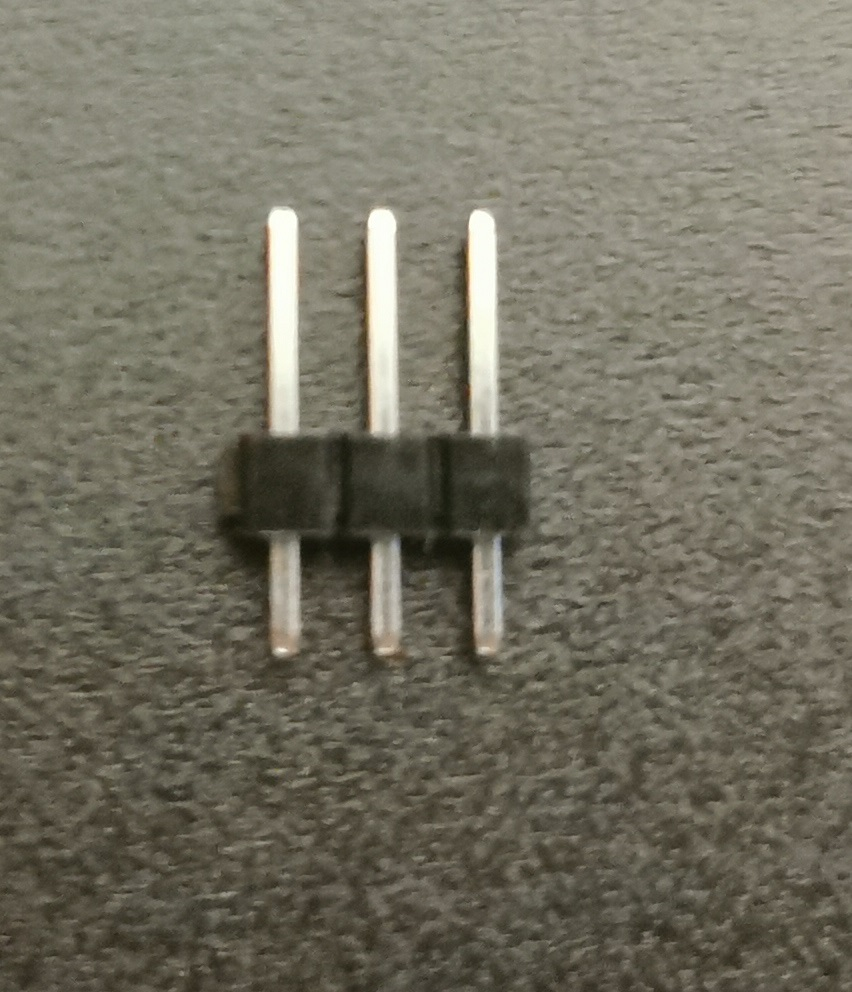
\includegraphics[width=\linewidth]{images/PinHeader.jpg}\captionof{figure}{The notches between the pins simplify separation}\label{fig:pinHeader}}%

With the pin headers, the process is very simple, since there is always a notch between the pins where the headers can be separated with a side cutter. Figure~\ref{fig:pinHeader} shows a three pin header with the clearly visible notches.%

With pin sockets this process is not as easy as with pin headers. Because of missing space there are no notches between the pins.%

For this reason it is necessary to first remove a pin with pliers, at which the strip should be separated. If a five pin socket is needed, the sixth pin is removed. Afterwards the socket is cut carefully with a side cutter at the now free place. This allows the sockets to be separated safely and reliably. The rough edges can be smoothed with the side cutter. The process is shown in figure~\ref{fig:pinSocket}.%

\begin{figure}[ht!]%
	\begin{centered}%
		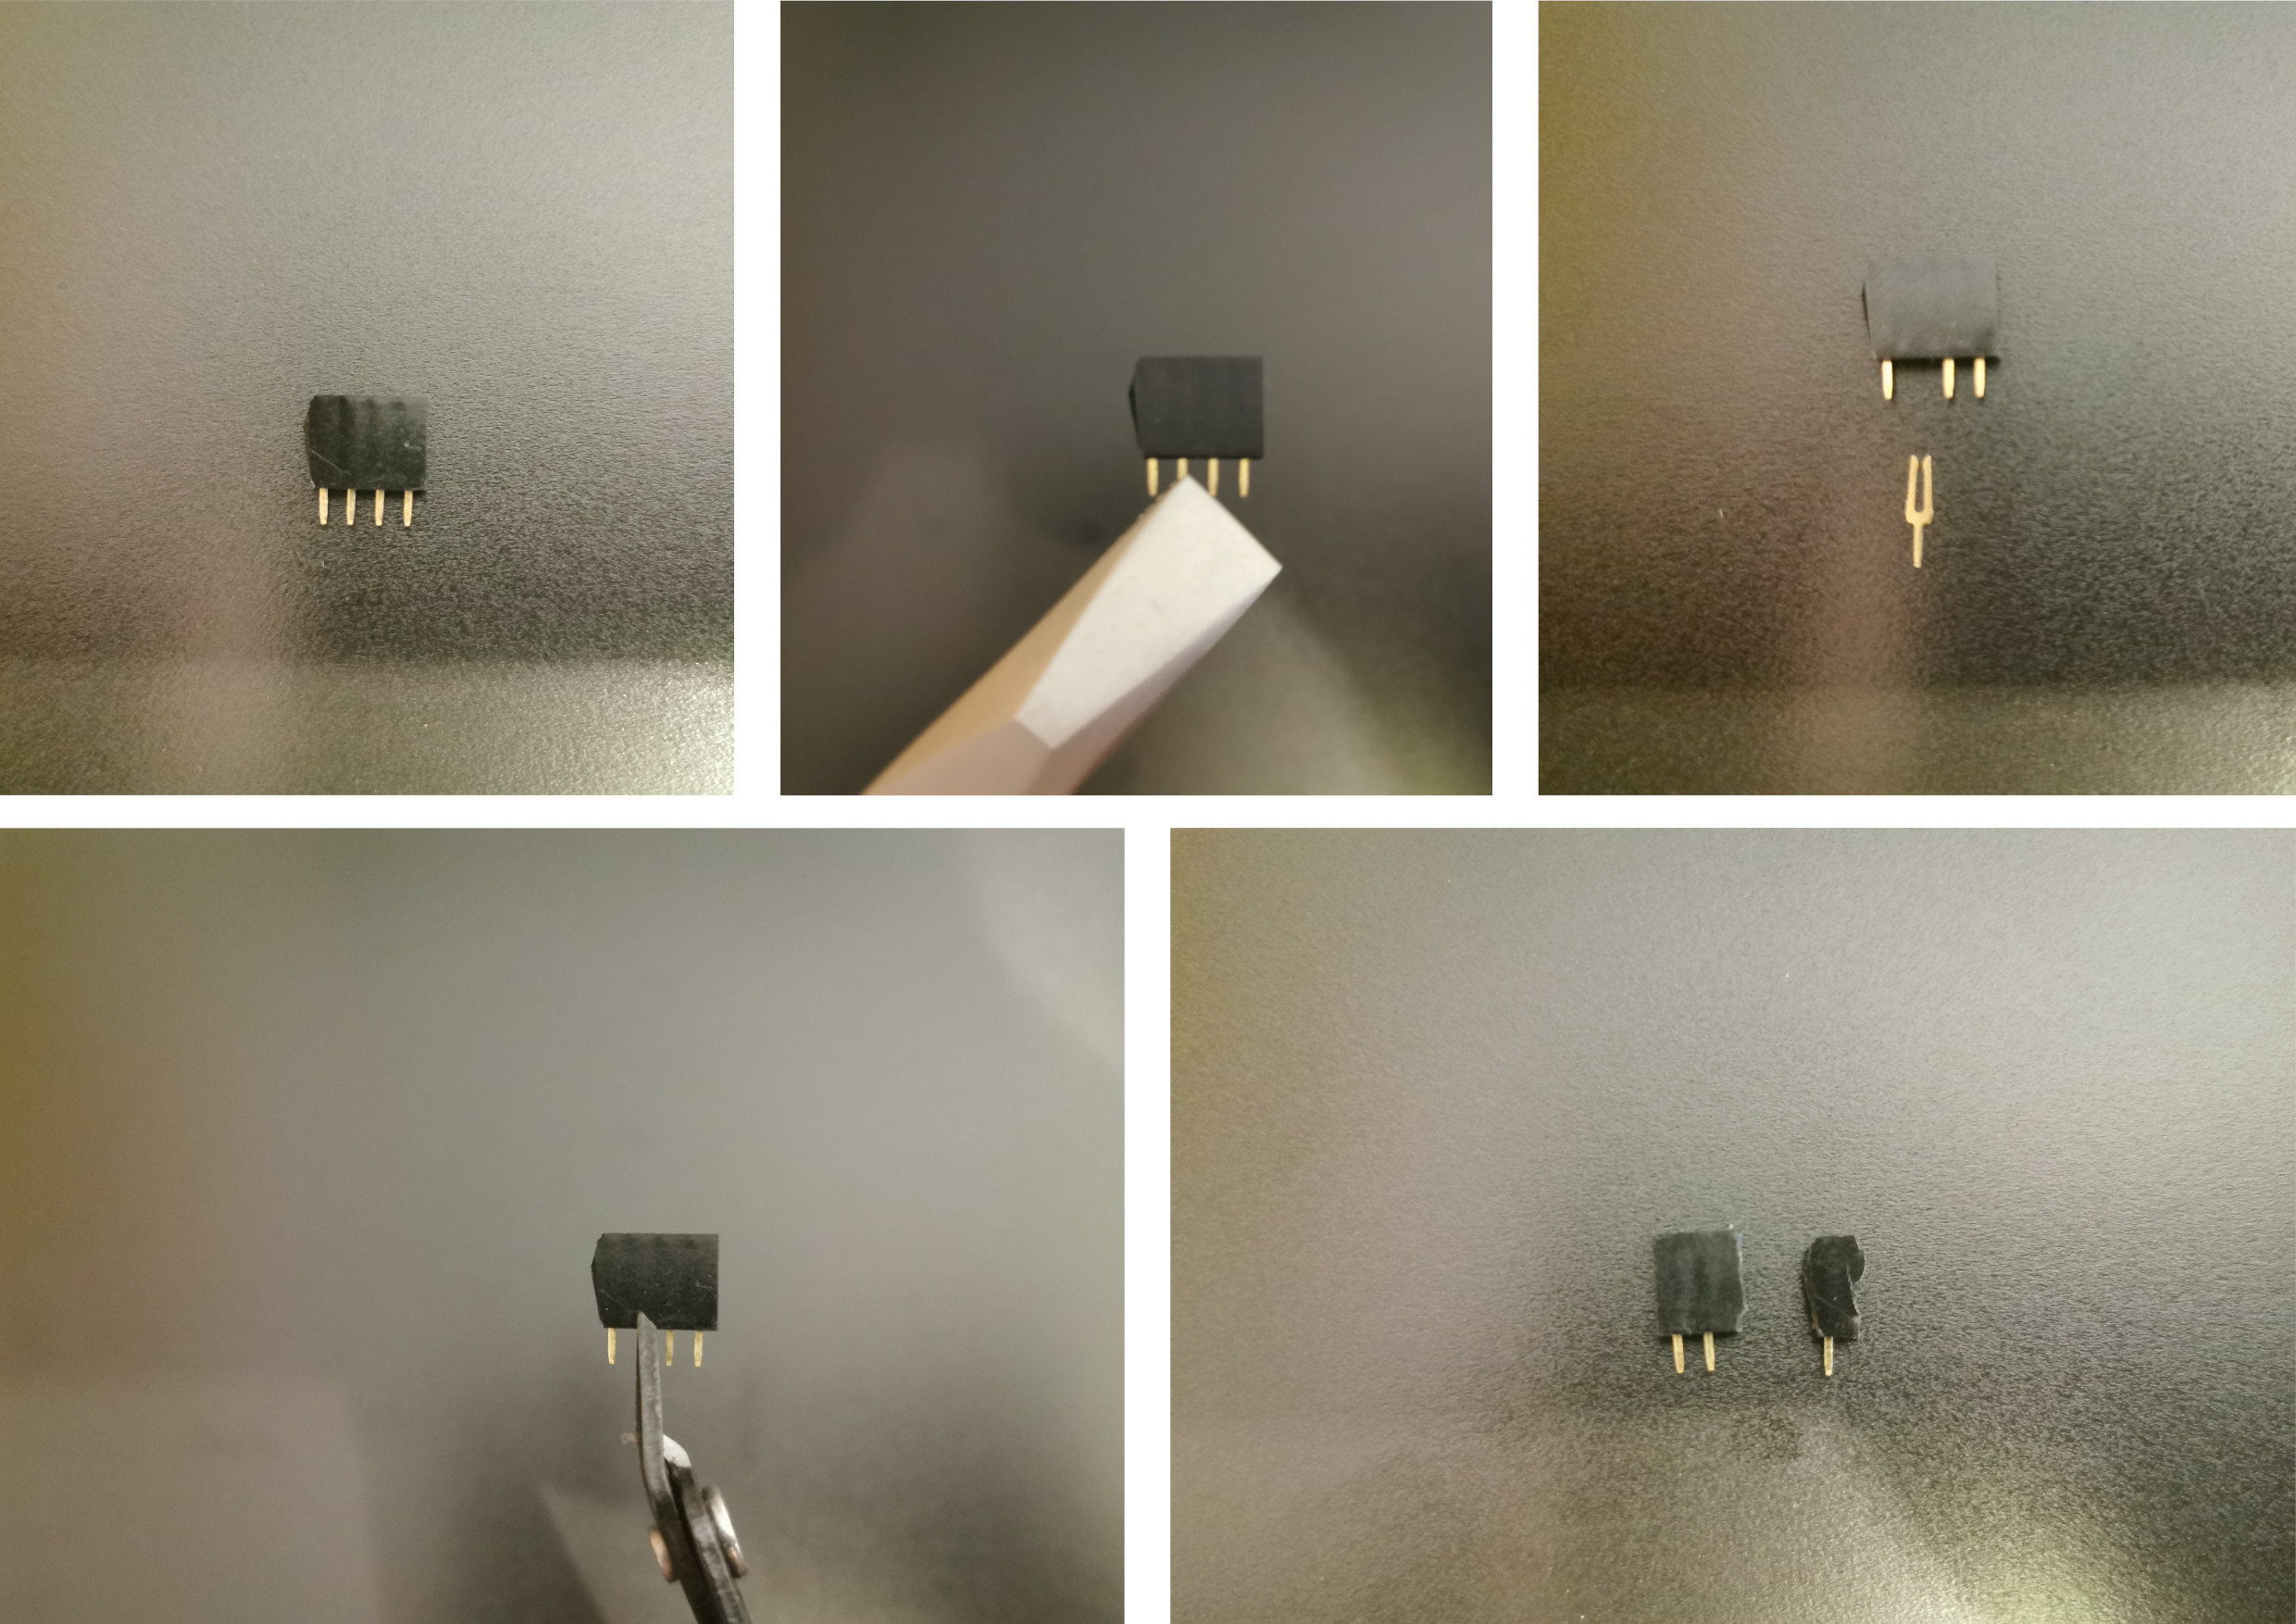
\includegraphics[width=\linewidth]{images/PinSocket.jpg}%
		\caption{How to separate pin sockets}%
		\label{fig:pinSocket}%
	\end{centered}%
\end{figure}%

\subsection{Assemble Pin Sockets}
The components which are mounted on pin sockets are the \hrefIdx{https://www.pololu.com/product/1182}{A4988 Stepper Drivers} and the \hrefIdx{https://www.espressif.com/en/products/hardware/esp32-devkitc/overview}{ESP32-DevKitC}.%

Both these components have two pin rows. It is therefore important that the pin sockets are mounted straight and parallel on the PCB so that the components can be inserted later.%

Without assistive tools, this is a pretty fiddly task. The simplest solution to this problem is to plug the pin sockets onto the corresponding components and solder them to the PCB. This ensures that the components fit exactly later.%

\subsection{TO-220 \& A4988 Cooling}%
The Open3DScanner does not use active cooling, but it is recommended to cool some parts passively.%

On the one hand the \hrefIdx{https://www.pololu.com/product/1182}{A4988 Stepper Drivers} should be equipped with a heat sink. If the stepper drivers get too warm, you may experience strange behavior (like missed steps). This is especially true if the stepper drivers are set to above \SI{1}{\ampere}.%

Furthermore, there are two \hrefIdx{https://www.centralsemi.com/PDFS/CASE/TO\_220\_PD.PDF}{TO-220} components on the board: the \hrefIdx{https://www.infineon.com/cms/en/product/power/mosfet/12v-300v-n-channel-power-mosfet/irlb8721/}{IRLB 8721} and the \hrefIdx{https://www.analog.com/en/products/lt1086.html}{LT1086CT-5}. The \hrefIdx{https://www.analog.com/en/products/lt1086.html}{LT1086CT-5} generates a lot of heat during operation, which can shorten the lifetime of the component considerably. For this reason I strongly recommend the use of thermal paste and a suitable heat sink.%

\marginElement{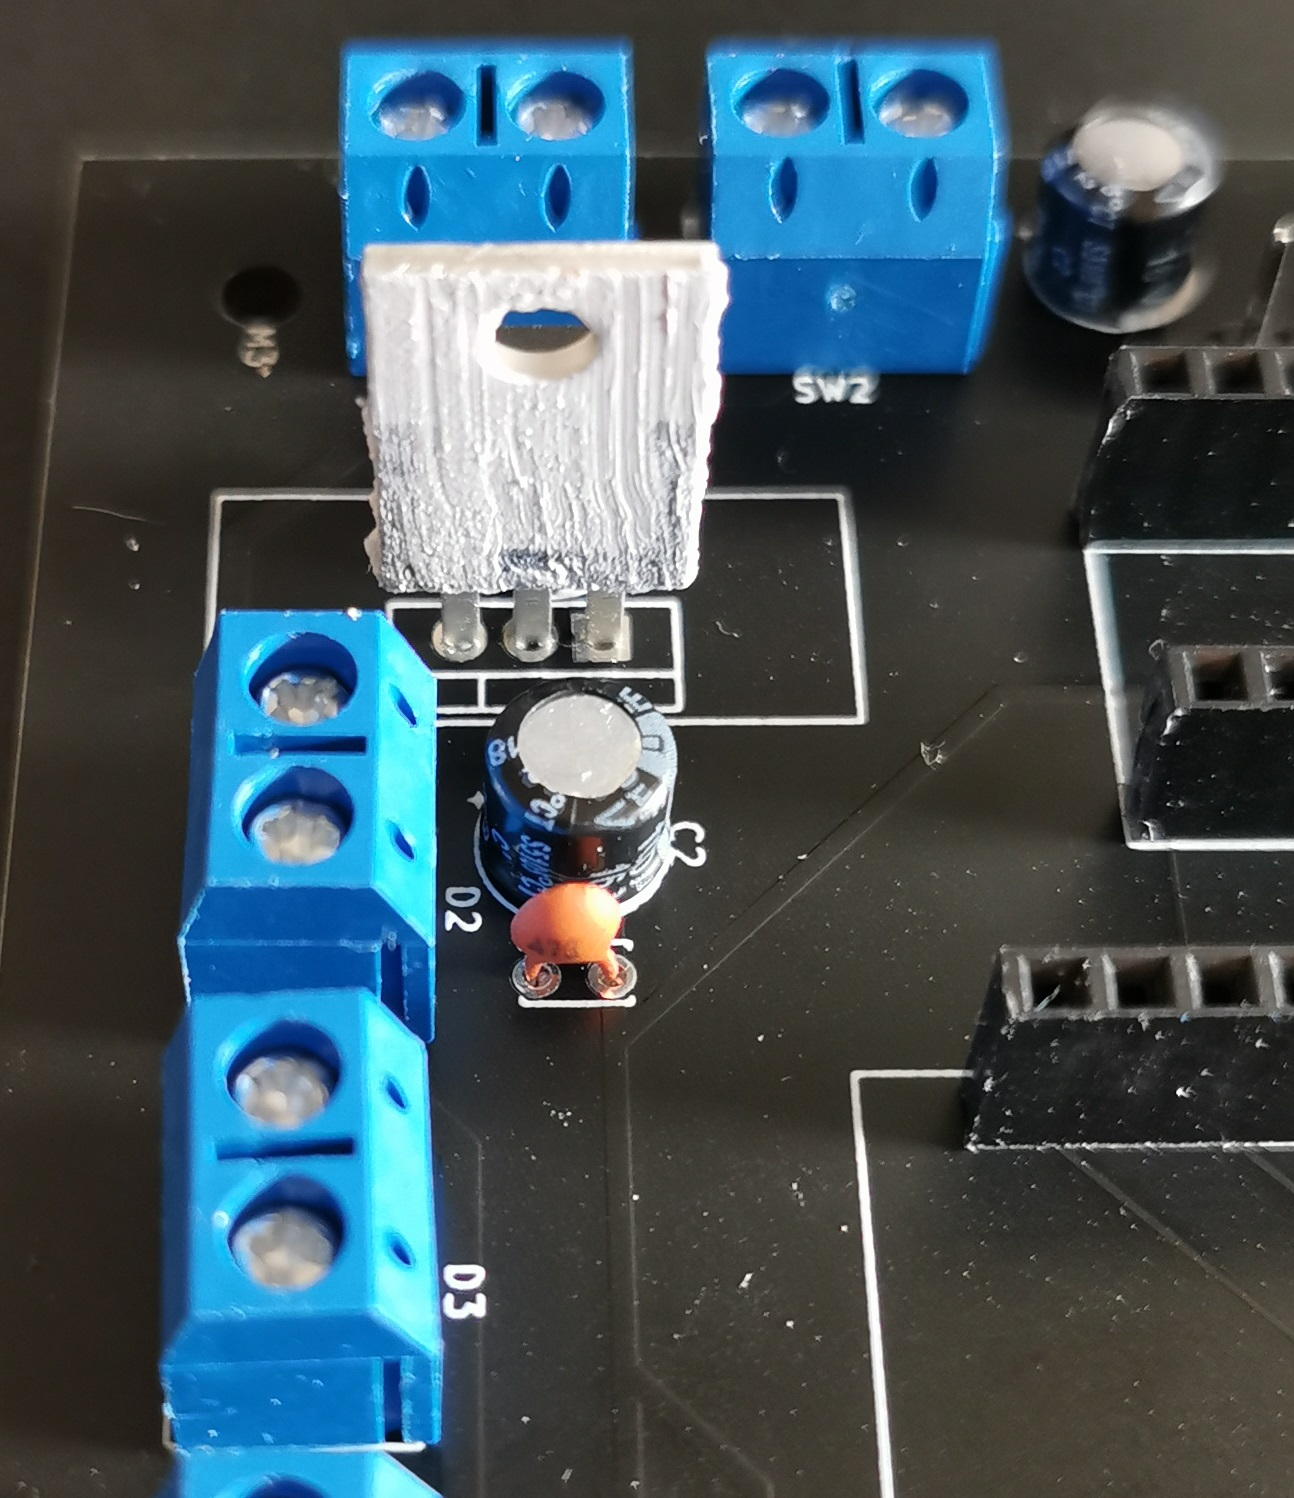
\includegraphics[width=\linewidth]{images/ThermalPaste.jpg}\captionof{figure}{Apply a thin layer of thermal paste\dots}}%
\marginElement{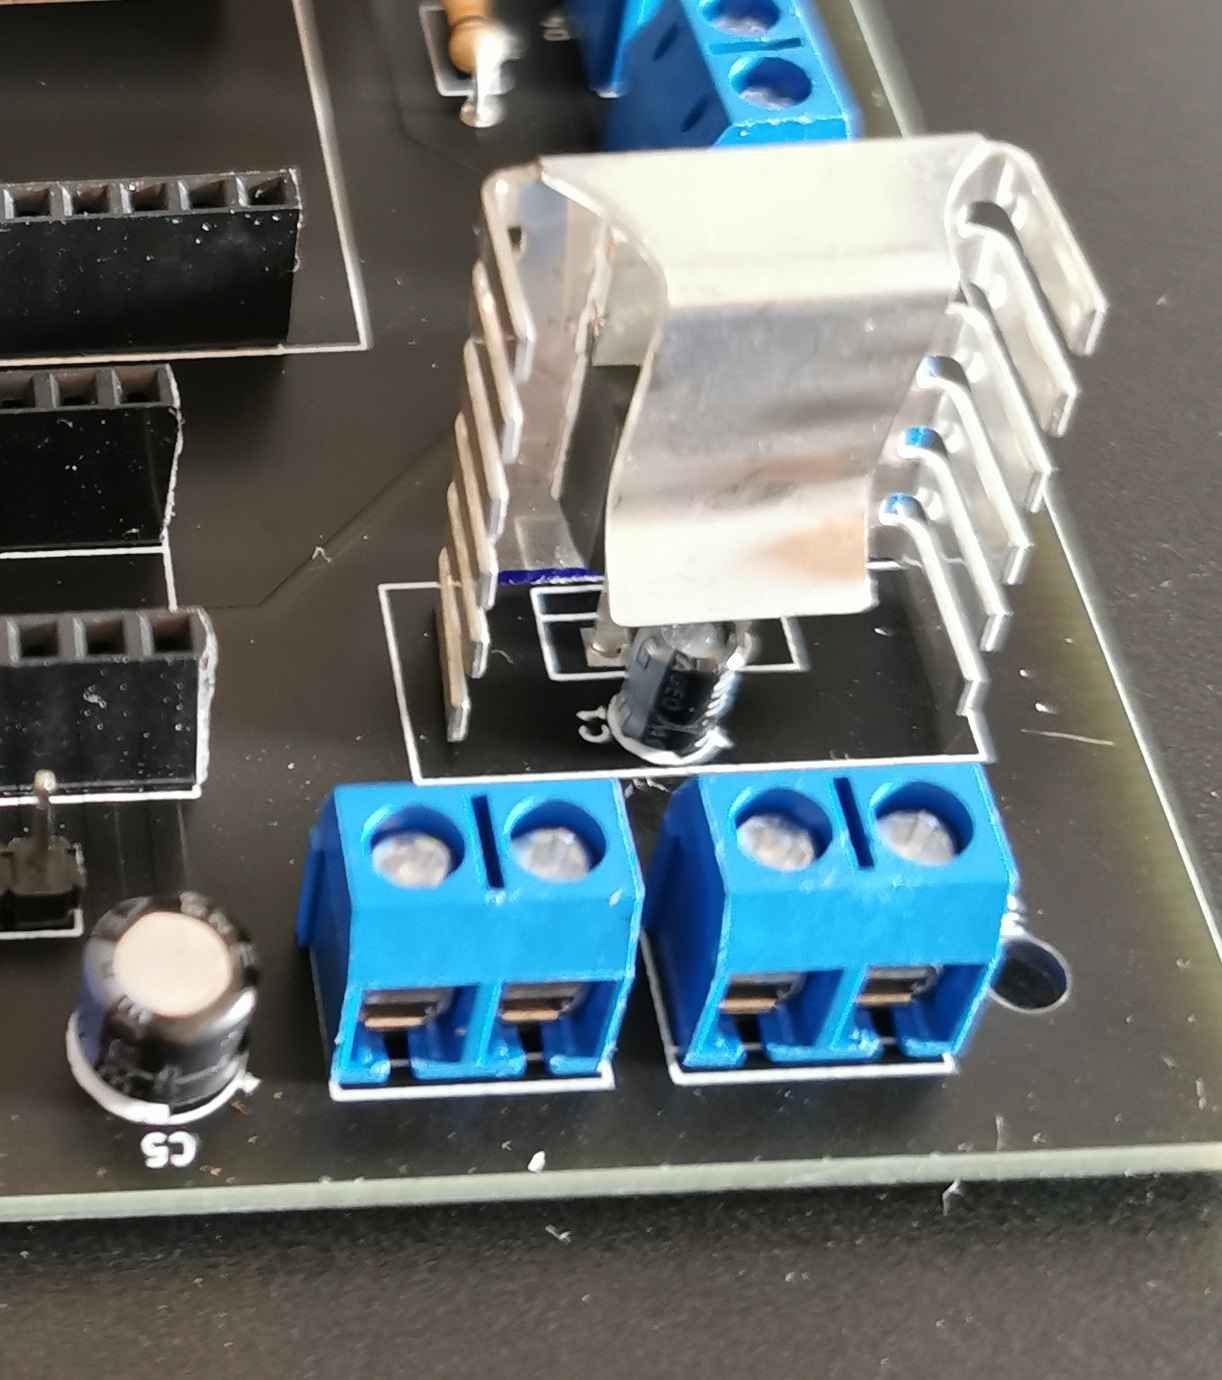
\includegraphics[width=\linewidth]{images/HeatSink.jpg}\captionof{figure}{\dots before installing the heat sink}}%

For the \hrefIdx{https://www.infineon.com/cms/en/product/power/mosfet/12v-300v-n-channel-power-mosfet/irlb8721/}{IRLB 8721} I didn't check to what extent it generates heat during operation, but according to the principle "better safe than sorry" I recommend the use of heat conducting paste and heat sink.%

Make sure that the heat sinks do not touch any other components or the circuit board. Especially with the \hrefIdx{https://www.analog.com/en/products/lt1086.html}{LT1086CT-5} it is a bit tight, because a high packing density is needed for an optimal function of the component.%

If you are using the TO-220 heat sinks I specified in the BOM, please note the following: Depending on how deep the pins are inserted into the PCB before soldering, it may be necessary to remove the bottom fin from the heat sink. Otherwise the heat sinks do not fit on the PCB, because they cannot put pressure on the component, which is necessary with the attachable heat sinks.%

\subsection{Prepare the LED Strip}%
The instructions in this section must be repeated for each light that will be connected to the Open3DScanner. While it is possible to operate the Open3DScanner with up to four lights simultaneously, I only use two.%

For the construction of the lights it is first necessary to prepare the LED strip. The LED strip is marked at regular intervals. At these markings it is possible to divide the strip.%

For the lights of the Open3DScanner \SI{15}{\centi\meter} long strips are needed. This corresponds to three segments of three LEDs. Figure~\ref{fig:ledStrip} shows such a \SI{15}{\centi\meter} piece of LED strip.%

\begin{figure}[ht!]%
	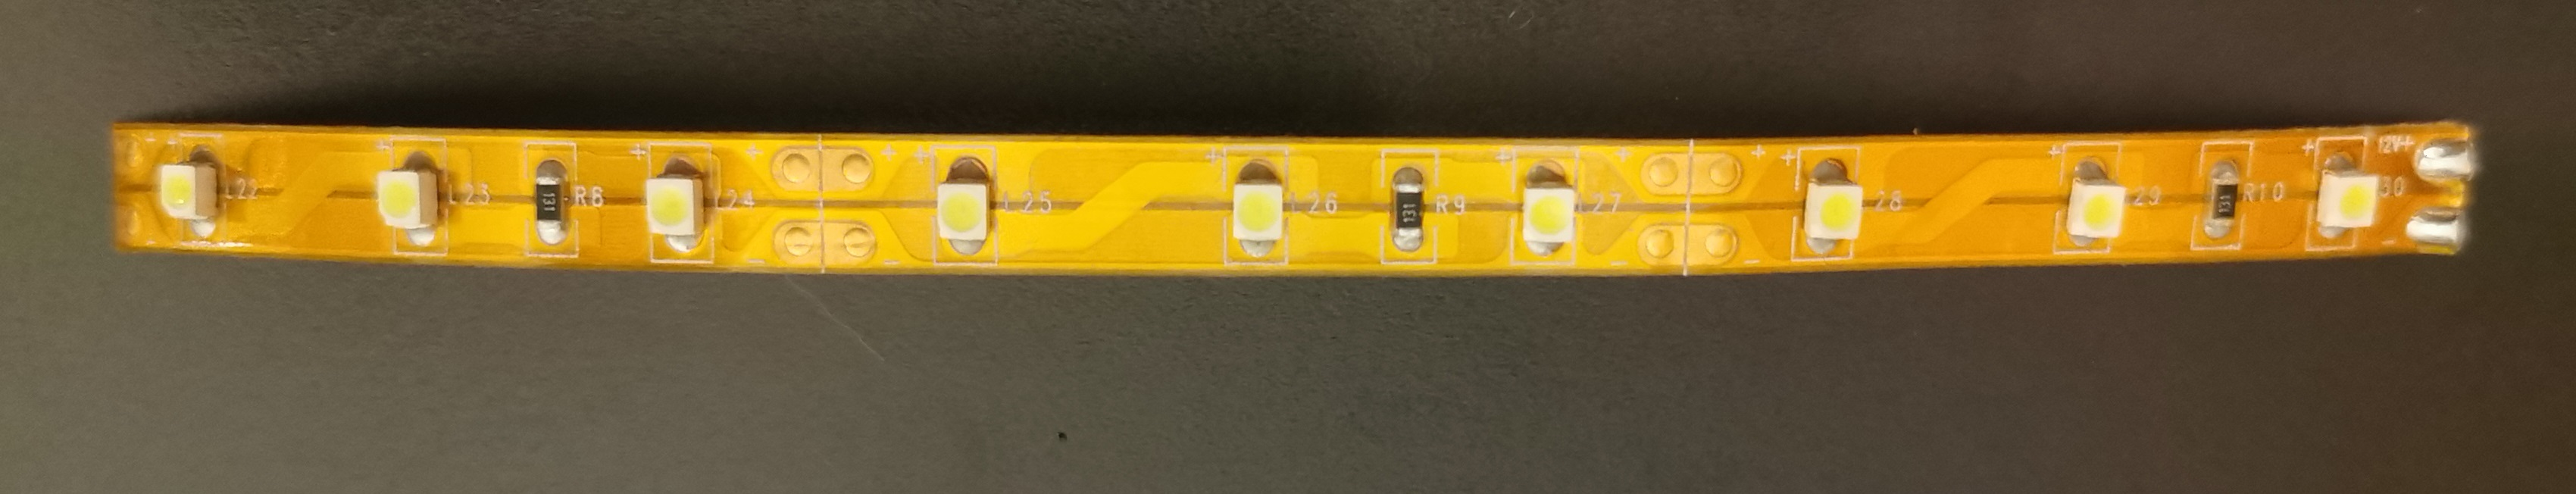
\includegraphics[width=\linewidth]{images/LedStrip.jpg}%
	\caption{One piece of LED strip as used in the Open3DScanner}%
	\label{fig:ledStrip}%
\end{figure}%

Each light of the Open3DScanner uses eight of these short strips and thus 72 LEDs.%

\begin{figure}[ht!]%
	\begin{centered}%
		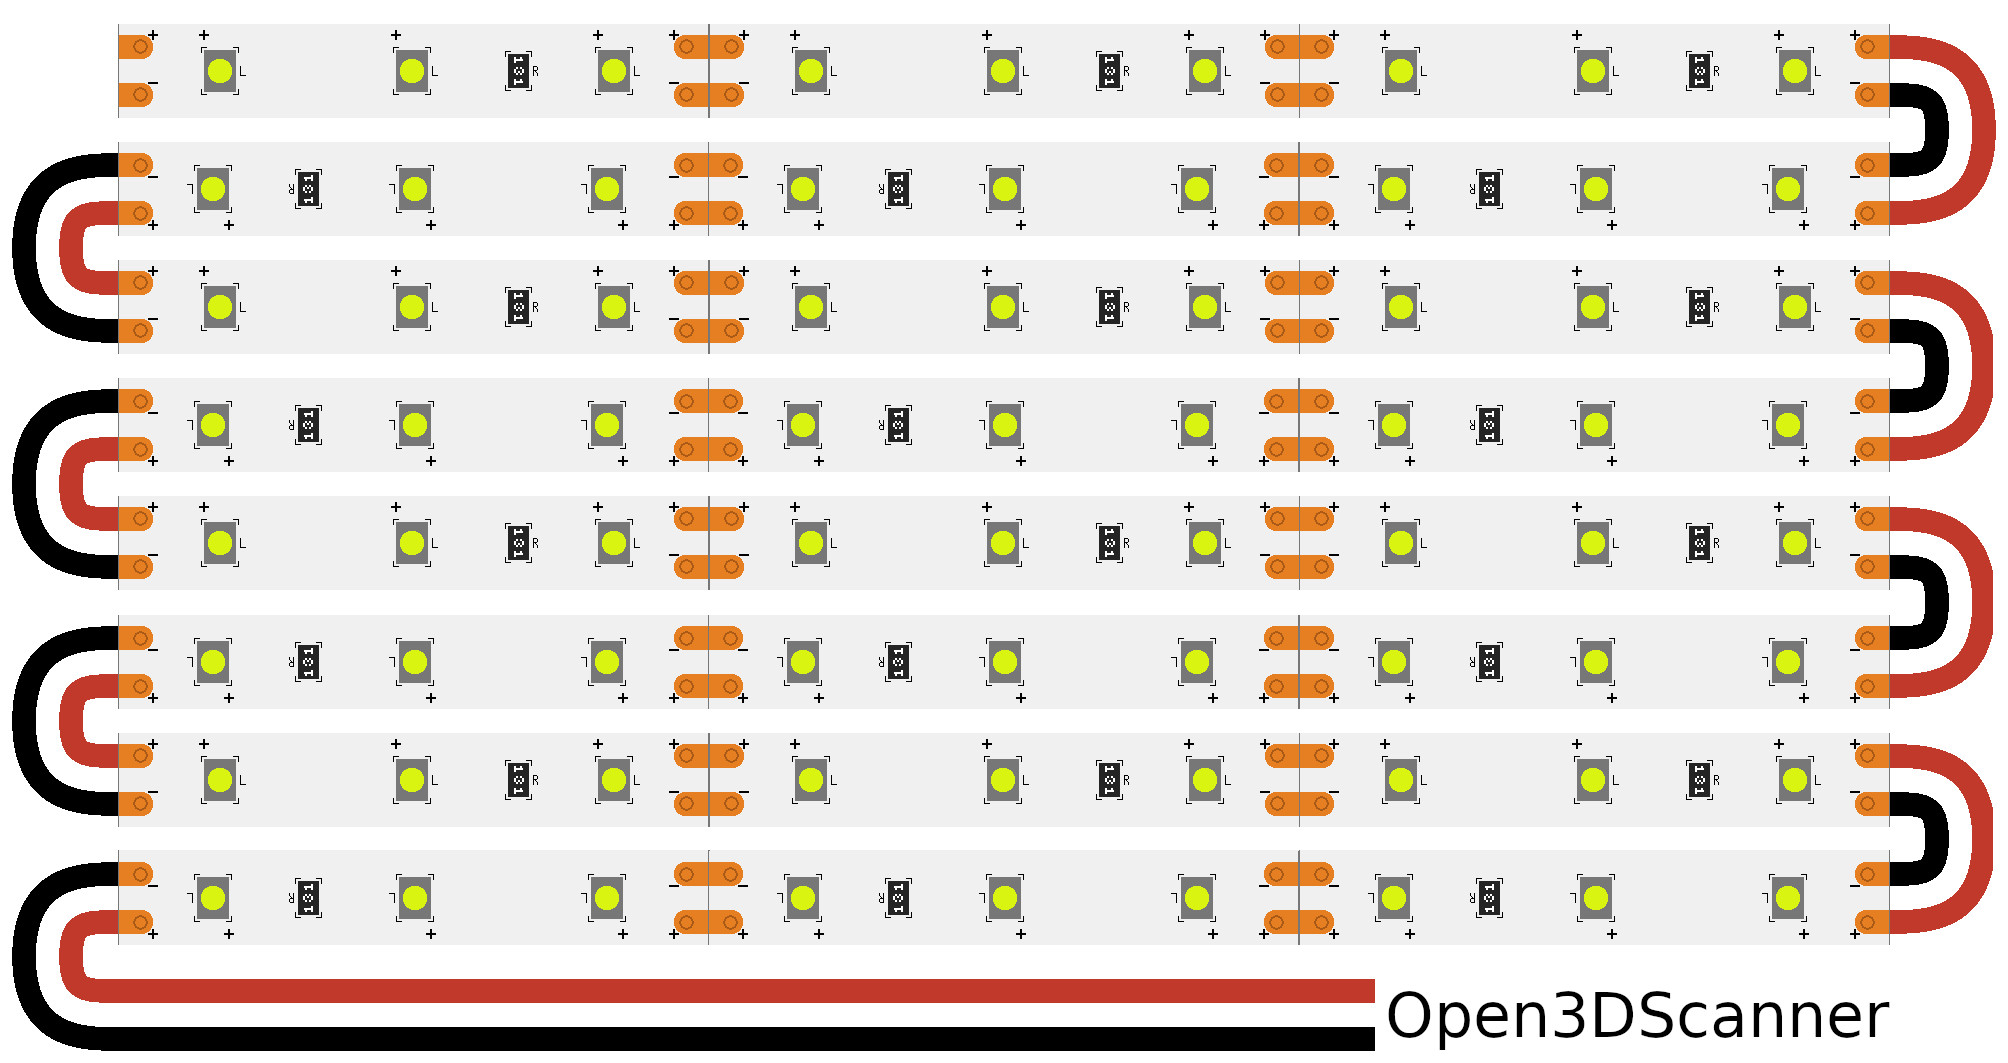
\includegraphics[width=\linewidth]{images/LedStripAssembly.jpg}%
		\caption{Schematic representation of the soldered LED strip for one light}%
		\label{fig:ledStripAssembly}%
	\end{centered}%
\end{figure}%

After dividing the LED Strip we need seven about \SI{7}{\centi\meter} long pieces of \SI{0.75}{\milli\meter\squared} cable with two wires each (for + and -). These are used to connect the segments of the LED strip to each other. We also need a approx. \SI{60}{\centi\meter} cable, which is used for the connection to the Open3DScanner. This cable can be shortened as soon as the lights are mounted and the cable is properly laid.%

Now the individual pieces of the LED strip are soldered together in series and the long cable is soldered to one end.%

It is important that no Molex connector is attached to the long cable at this point, otherwise we will not be able to lay the cable as intended. In general, it makes sense to attach the connector after the cable has been shortened to the correct length.%

A schematic representation of how the result of the soldering should look like can be found in figure~\ref{fig:ledStripAssembly}. When soldering, be sure to connect the right contacts.%

Now the soldered LED strip is glued to the Spotlight-Frame. One strip is glued in the middle of each of the recesses. Make sure that the long cable is at the lower end.%

\marginElement{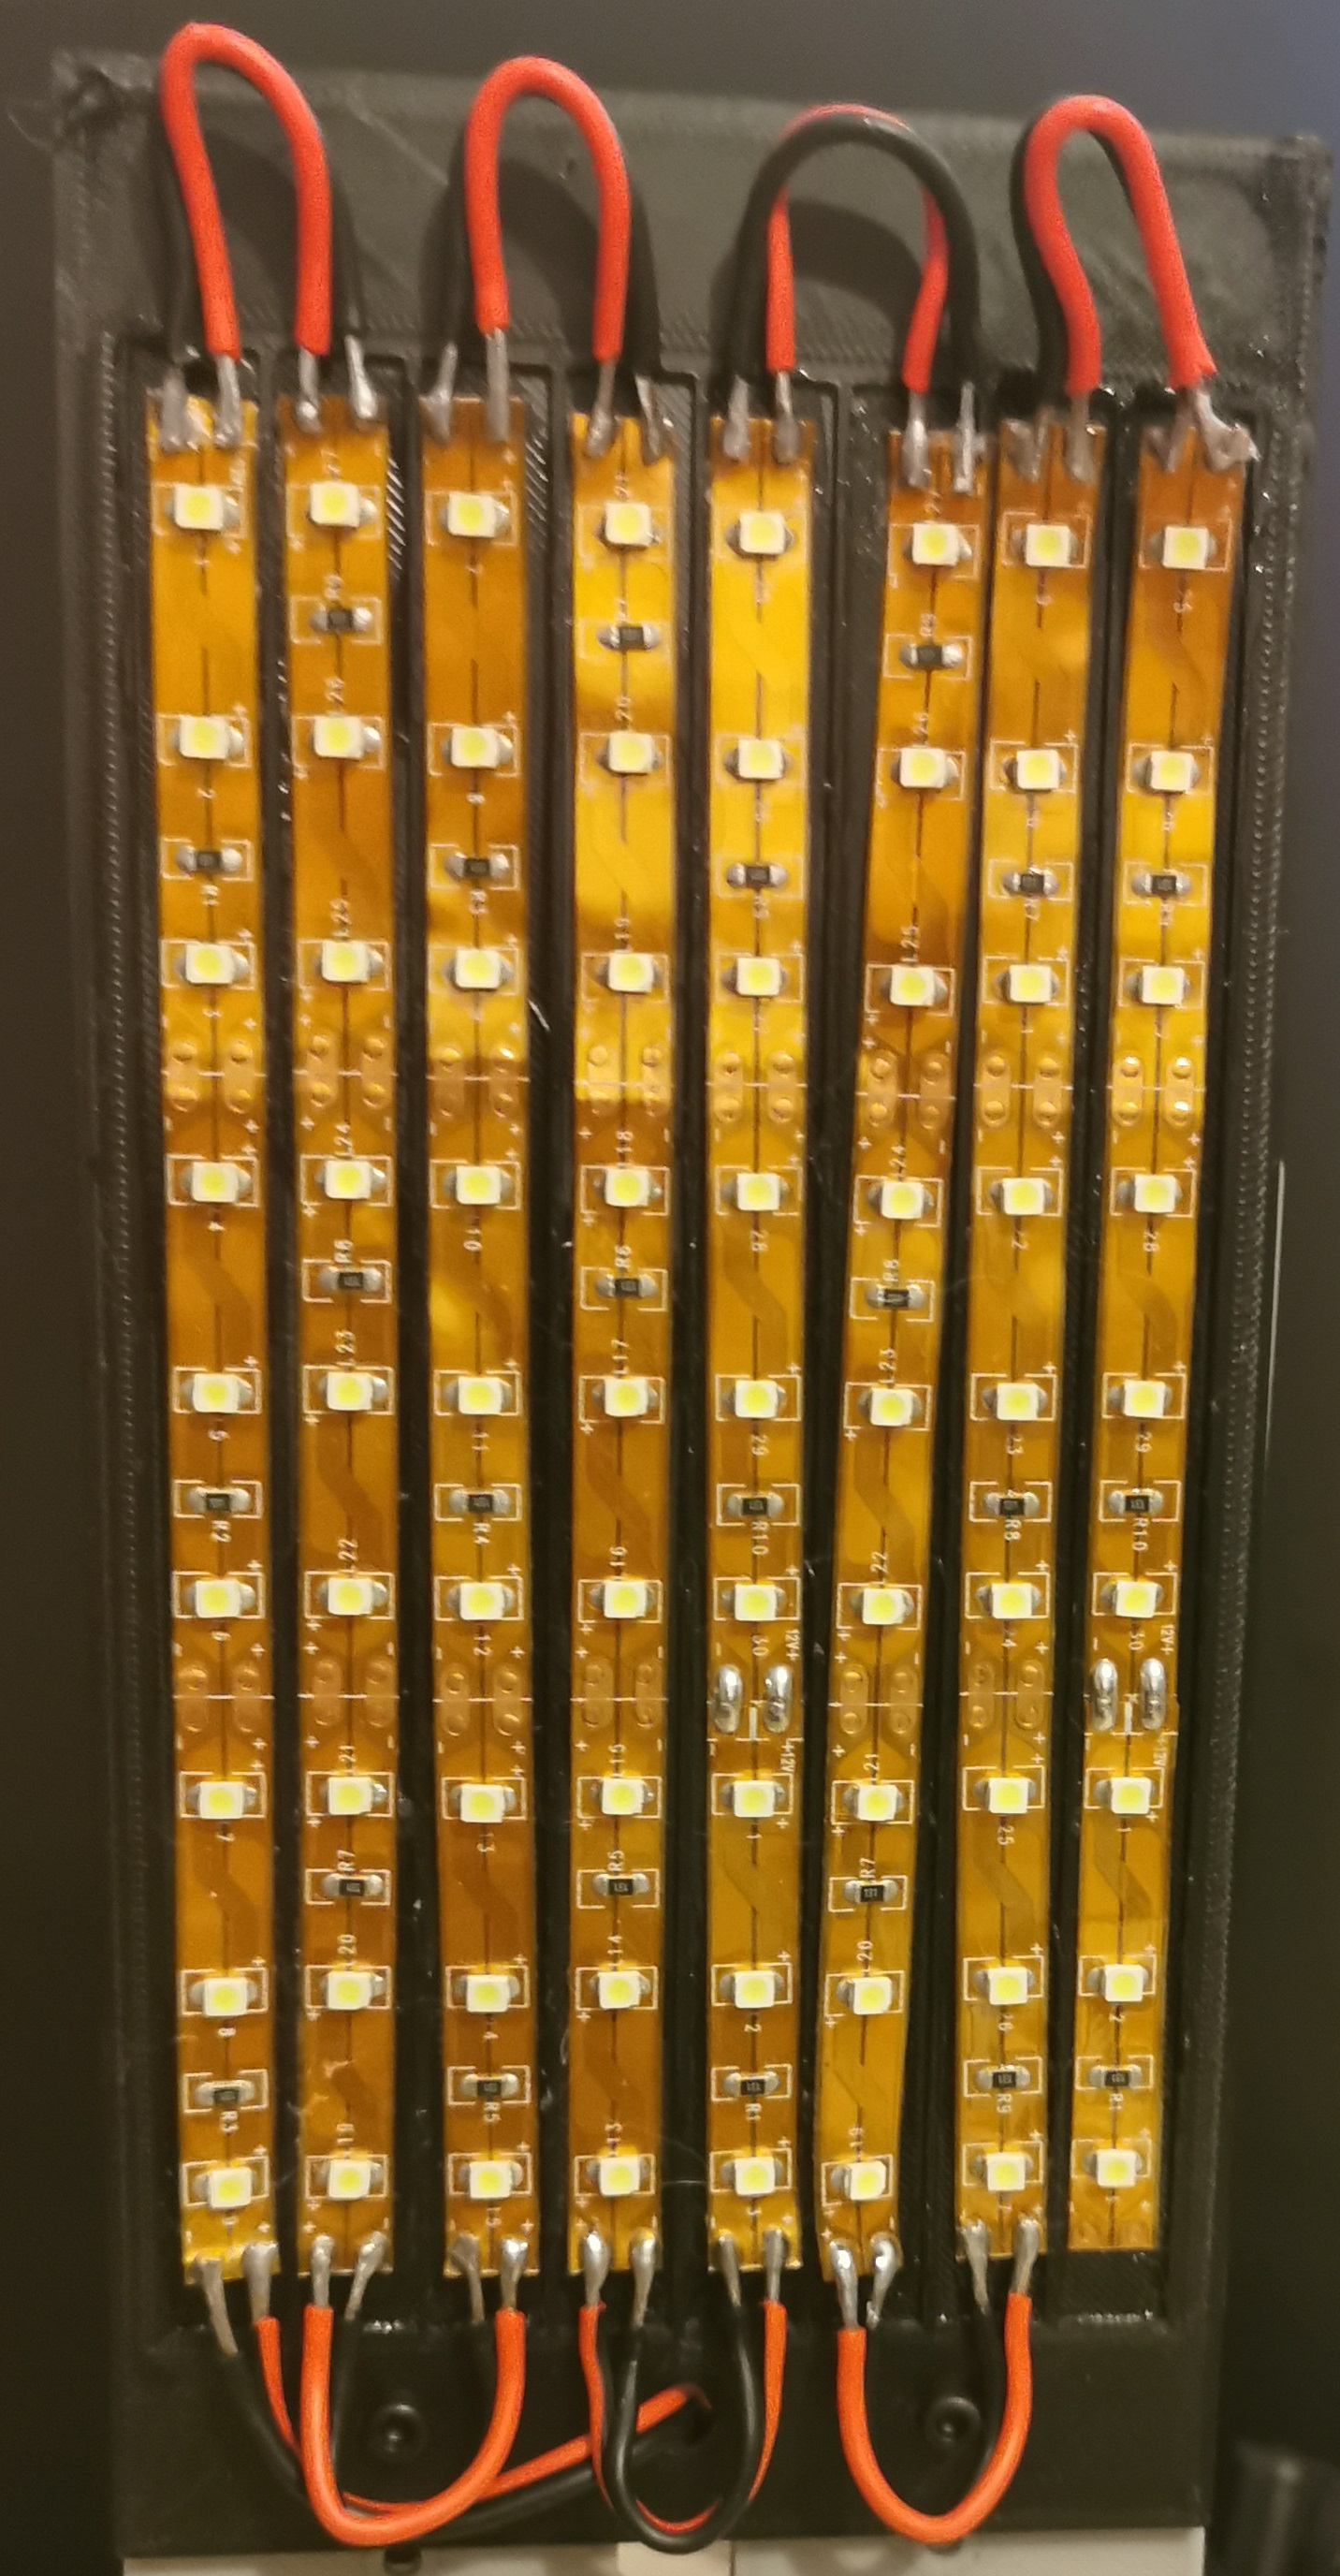
\includegraphics[width=\linewidth]{images/LedStripGlue.jpg}\captionof{figure}{Soldered LED strip glued into printed part}\label{fig:ledStripGlue}}%

The end of the long cable is led through the hole, which is in the lower area, in the middle of the part. Figure~\ref{fig:ledStripGlue} shows what the result should look like.%

The LED strip is glued in with the pre-assembled M3 adhesive tape. If this is not strong enough and the LED strips come loose again, you can simply spread some liquid glue on the printed part and then press the LED strip in again.

The LED strip is now ready for the assembly of the light which is described in section~\ref{sec:assembly}.

\subsection{Preparing the Cables}
In this section the cables used in the Open3DScanner are described in more detail. This is explicitly not a manual for crimping, there are very good sources for this\sideNote{There are many good instructions for crimping various connections on the Internet. For example, for crimping \hrefIdx{https://www.instructables.com/id/Dupont-Crimp-Tool-Tutorial/}{Dupont cables}, \hrefIdx{https://www.molex.com/molex/common/staticLoader.jsp?fileName=/tnotes/crimp.html\&progLink=Good+Crimps\&\&channel=...Micro-Fit\&channelId=0}{Molex Micro Fit}, and \hrefIdx{https://www.klauke.com/en/electrical/sectors-solutions/technical-reports/crimping-cable-lugs-correctly/}{cable lugs}. {\faYoutube} \hrefIdx{https://www.youtube.com/results?search\_query=crimping+tutorial}{YouTube} is a great source for tutorials, too.}.%

Instead, the following paragraphs describe the individual cables and their connections.%

A schematic diagram is given for each cable, which clearly shows how cables are aligned, if necessary.%

Power cables are shown in red (+) and black (GND), while all data cables are shown in blue. This colour coding is reused in later illustrations and thus simplifies orientation.%

The cable lengths specified do not include the length of the connectors which are used for each cable.%

\paragraph{LED Strip}\mbox{}\\%

\sideTabularx[LED strip cable characteristics]{%
	\rowcolors{2}{tableLineTwo}{tableLineOne}% specify rowcolors in tabularx style
	\begin{tabularx} {\marginparwidth} {>{\rowmac \hsize=\hsize}X>{\rowmac \hsize=\hsize}X<{\clearrow}}%
		\tabularxHeader%
		Characteristic & Value\\%
		Quantity & 4\\%
		Wire Gauge & \SI{0.75}{\milli\meter\squared}\\%
		Length & \SI{15}{\centi\meter}\\%
		End A Connector & Ferrule Crimp\\%
		End B Connector & Micro-Fit - 1x2-pin, male\\%
		End A connects & PCB contacts D2, D3, D4, D5\\%
		End B connects & Open3DScanner housing\\%
	\end{tabularx}%
}%

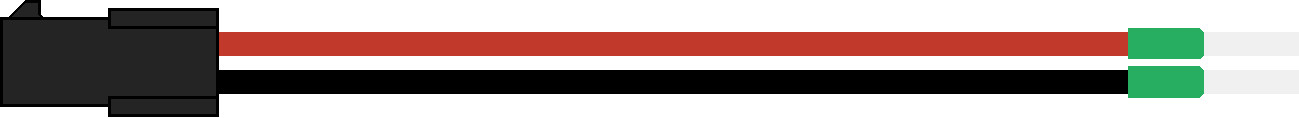
\includegraphics[width=\linewidth]{images/LedStripCable.jpg}%
{\captionof{figure}{Schematic representation of the LED strip cable}}% Take note of the surrounding {} to encapsulate special format settings

During assembly, the Molex connectors are clamped into the housing of the Open3DScanner so that they are directly accessible from the outside and the lights can be connected with a suitable Molex plug.%

Since ferrule crimps are necessary for the \SI{0.75}{\milli\meter\squared} cables, they may sit very tight in the screw terminals afterwards, which is no problem.%

Even if no or less than four lights will be connected to the Open3DScanner, it is necessary to prepare four of these cables so that there will be no gaps in the case later.%

The corresponding female connectors need to be added to the LED strips. This cable is not shown here. Just ensure that the polarity matches these cables.%

\clearpage%

\paragraph{Power Cables}\mbox{}\\%

\sideTabularx[Power connection cable characteristics]{%
	\rowcolors{2}{tableLineTwo}{tableLineOne}% specify rowcolors in tabularx style
	\begin{tabularx} {\marginparwidth} {>{\rowmac \hsize=\hsize}X>{\rowmac \hsize=\hsize}X<{\clearrow}}%
		\tabularxHeader%
		Characteristic & Value\\%
		Quantity & 2\\%
		Wire Gauge & \SI{0.75}{\milli\meter\squared}\\%
		Length & \SI{16/20}{\centi\meter} (Power Jack/Rocker Switch)\\%
		End A Connector & Ferrule Crimp\\%
		End B Connector & Cable Lug\\%
		End A connects & PCB contacts J1, SW2\\%
		End B connects & Rocker Switch \& Power Jack\\%
	\end{tabularx}%
}%

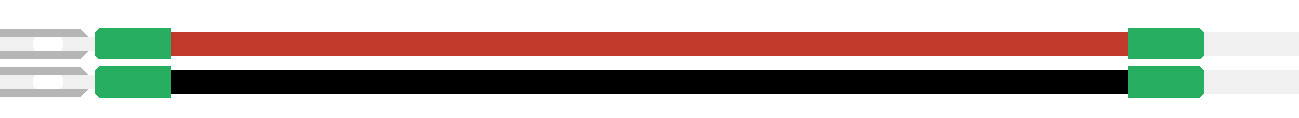
\includegraphics[width=\linewidth]{images/PowerCable.jpg}%
{\captionof{figure}{Schematic representation of the power connection cable}}% Take note of the surrounding {} to encapsulate special format settings

Two identical cables are used to connect the power source to the PCB and to connect the rocker switch, which allows the device to be switched on and off.%

Make sure that the correct cable lugs are used for both cables. These can be different for different versions of the parts and must be selected appropriately for the components.%

\paragraph{USB Cable}\mbox{}\\%

\sideTabularx[USB cable characteristics]{%
	\rowcolors{2}{tableLineTwo}{tableLineOne}% specify rowcolors in tabularx style
	\begin{tabularx} {\marginparwidth} {>{\rowmac \hsize=\hsize}X>{\rowmac \hsize=\hsize}X<{\clearrow}}%
		\tabularxHeader%
		Characteristic & Value\\%
		Quantity & 1\\%
		Wire Gauge & Undefined\\%
		Length & \SI{15}{\centi\meter}\\%
		End A Connector & Ferrule Crimp\\%
		End B Connector & Micro USB-B\\%
		End A connects & PCB contact J2\\%
		End B connects & \hrefIdx{https://www.espressif.com/en/products/hardware/esp32-devkitc/overview}{ESP32-DevKitC}\\%
	\end{tabularx}%
}%

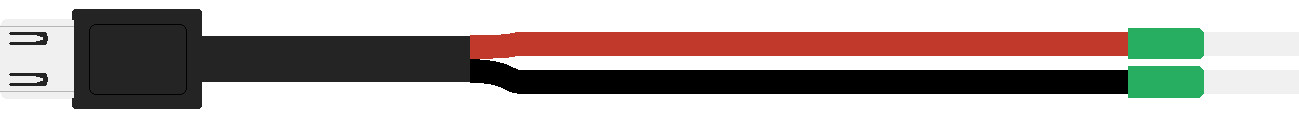
\includegraphics[width=\linewidth]{images/UsbCable.jpg}%
{\captionof{figure}{Schematic representation of the USB cable}}% Take note of the surrounding {} to encapsulate special format settings

Since an \hrefIdx{https://www.espressif.com/en/products/hardware/esp32-devkitc/overview}{ESP32-DevKitC} is used in the Open3DScanner, it is necessary to supply it with power via the Micro-USB-B socket.%

The cable diameter for the USB cable is not specified as any USB cable can be used to power the ESP32. The available USB cables on the market have different cable diameters, but it is not necessary to buy a special cable.%

\paragraph{Bi-Color LED Cable}\mbox{}\\%

\sideTabularx[Bi-color LED cable characteristics]{%
	\rowcolors{2}{tableLineTwo}{tableLineOne}% specify rowcolors in tabularx style
	\begin{tabularx} {\marginparwidth} {>{\rowmac \hsize=\hsize}X>{\rowmac \hsize=\hsize}X<{\clearrow}}%
		\tabularxHeader%
		Characteristic & Value\\%
		Quantity & 1\\%
		Wire Gauge & \SI{0.2}{\milli\meter\squared}\\%
		Length & \SI{11}{\centi\meter}\\%
		End A Connector & 3-Pin Dupont\\%
		End B Connector & 3-Pin Dupont\\%
		End A connects & PCB contact D1\\%
		End B connects & Bi-color LED\\%
	\end{tabularx}%
}%

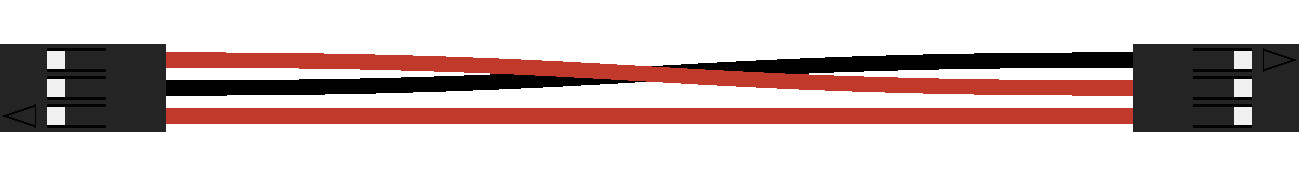
\includegraphics[width=\linewidth]{images/DualColorLedCable.jpg}%
{\captionof{figure}{Schematic representation of the bi-color LED cable}}% Take note of the surrounding {} to encapsulate special format settings

The bi-color LED is plugged directly into the Dupont connector.%

When assembling this cable it is important to pay attention to the cable assignment. The two plugs are not connected identically.%

\clearpage%

\paragraph{Encoder Cable}\mbox{}\\%

\sideTabularx[Encoder cable characteristics]{%
	\rowcolors{2}{tableLineTwo}{tableLineOne}% specify rowcolors in tabularx style
	\begin{tabularx} {\marginparwidth} {>{\rowmac \hsize=\hsize}X>{\rowmac \hsize=\hsize}X<{\clearrow}}%
		\tabularxHeader%
		Characteristic & Value\\%
		Quantity & 1\\%
		Wire Gauge & \SI{0.2}{\milli\meter\squared}\\%
		Length & \SI{15}{\centi\meter}\\%
		End A Connector & 3-Pin Dupont\\%
		End B Connector & 2$\times$3-Pin Dupont\\%
		End A connects & PCB contact SW1\\%
		End B connects & Rotary Encoder\\%
	\end{tabularx}%
}%

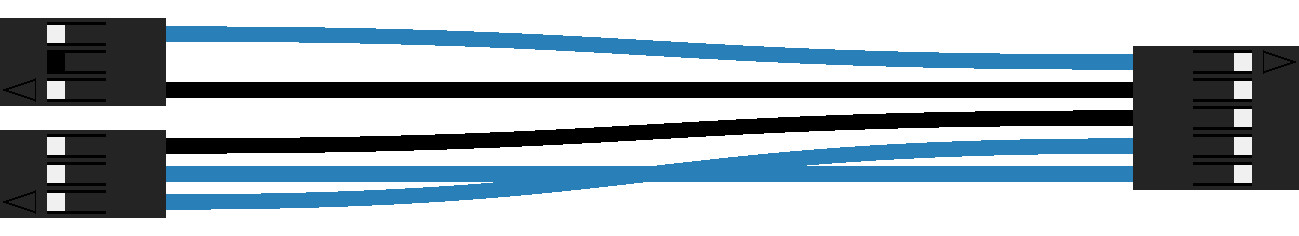
\includegraphics[width=\linewidth]{images/EncoderCable.jpg}%
{\captionof{figure}{Schematic representation of the encoder cable}}% Take note of the surrounding {} to encapsulate special format settings

As with the bi-color LED, the cable for the encoder is connected directly to the component. However, there is a special aspect here which is given by the pin layout of the encoder used.%

The pins of the encoder are arranged in two rows (2 + 3). The pins of the 2-series are arranged like a 3-series, where the middle pin is missing. For this reason, two 3-pin Dupont housings are used on the component side, where one space remains unoccupied.%

\paragraph{Display Cable}\mbox{}\\%

\sideTabularx[Display cable characteristics]{%
	\rowcolors{2}{tableLineTwo}{tableLineOne}% specify rowcolors in tabularx style
	\begin{tabularx} {\marginparwidth} {>{\rowmac \hsize=\hsize}X>{\rowmac \hsize=\hsize}X<{\clearrow}}%
		\tabularxHeader%
		Characteristic & Value\\%
		Quantity & 1\\%
		Wire Gauge & \SI{0.2}{\milli\meter\squared}\\%
		Length & \SI{15}{\centi\meter}\\%
		End A Connector & 8-Pin Dupont\\%
		End B Connector & 8-Pin Dupont\\%
		End A connects & PCB contact DS1\\%
		End B connects & Display\\%
	\end{tabularx}%
}%

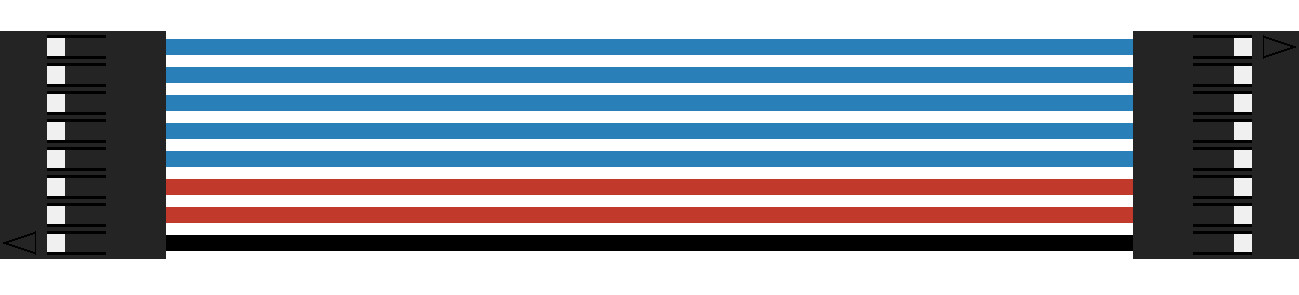
\includegraphics[width=\linewidth]{images/DisplayCable.jpg}%
{\captionof{figure}{Schematic representation of the display cable}}% Take note of the surrounding {} to encapsulate special format settings

Since the used display is mounted on a printed circuit board, the cable is connected to the two pin headers on the display and the PCB.

\section{Assembly the Open3DScanner}%
\label{sec:assembly}
After all the necessary preparatory work has been done, the actual instructions for building the Open3DScanner follow.%

Each individual step is illustrated by an figure. In addition, each step is provided with a short instruction and, if useful, further tips, warnings and notes are given.%

At each step all used components are listed. If these partially assembled parts are subsequently used in further steps, they will not be listed again.%

At the end there are further illustrations, which contain exact dimensions and orientations of parts.%
\clearpage%

% STEP 1
\sideTabularx[Required parts for step 1]{%
	\rowcolors{2}{tableLineTwo}{tableLineOne}% specify rowcolors in tabularx style
	\begin{tabularx} {\marginparwidth} {>{\rowmac \hsize=1.5\hsize}X>{\rowmac \hsize=0.5\hsize}X<{\clearrow}}%
		\tabularxHeader%
		Part & Quantity\\%
		Rotor-Stand & 1\\%
		Passive-Stand & 1\\%
		625ZZ Bearing & 2\\%
	\end{tabularx}%
}%

\marginInfo*[Instructions]{Press one bearing into each of the openings provided in the upper area of the printed parts. The bearings should be flush with the surface of the printed parts.}%

\marginTips*[Tip]{If the opening for the bearings is a tad too tight, you can use pliers to press the bearings into the opening. In this case a piece of fabric or tissue should be placed between the pliers and the components to avoid craters and deformation.}%

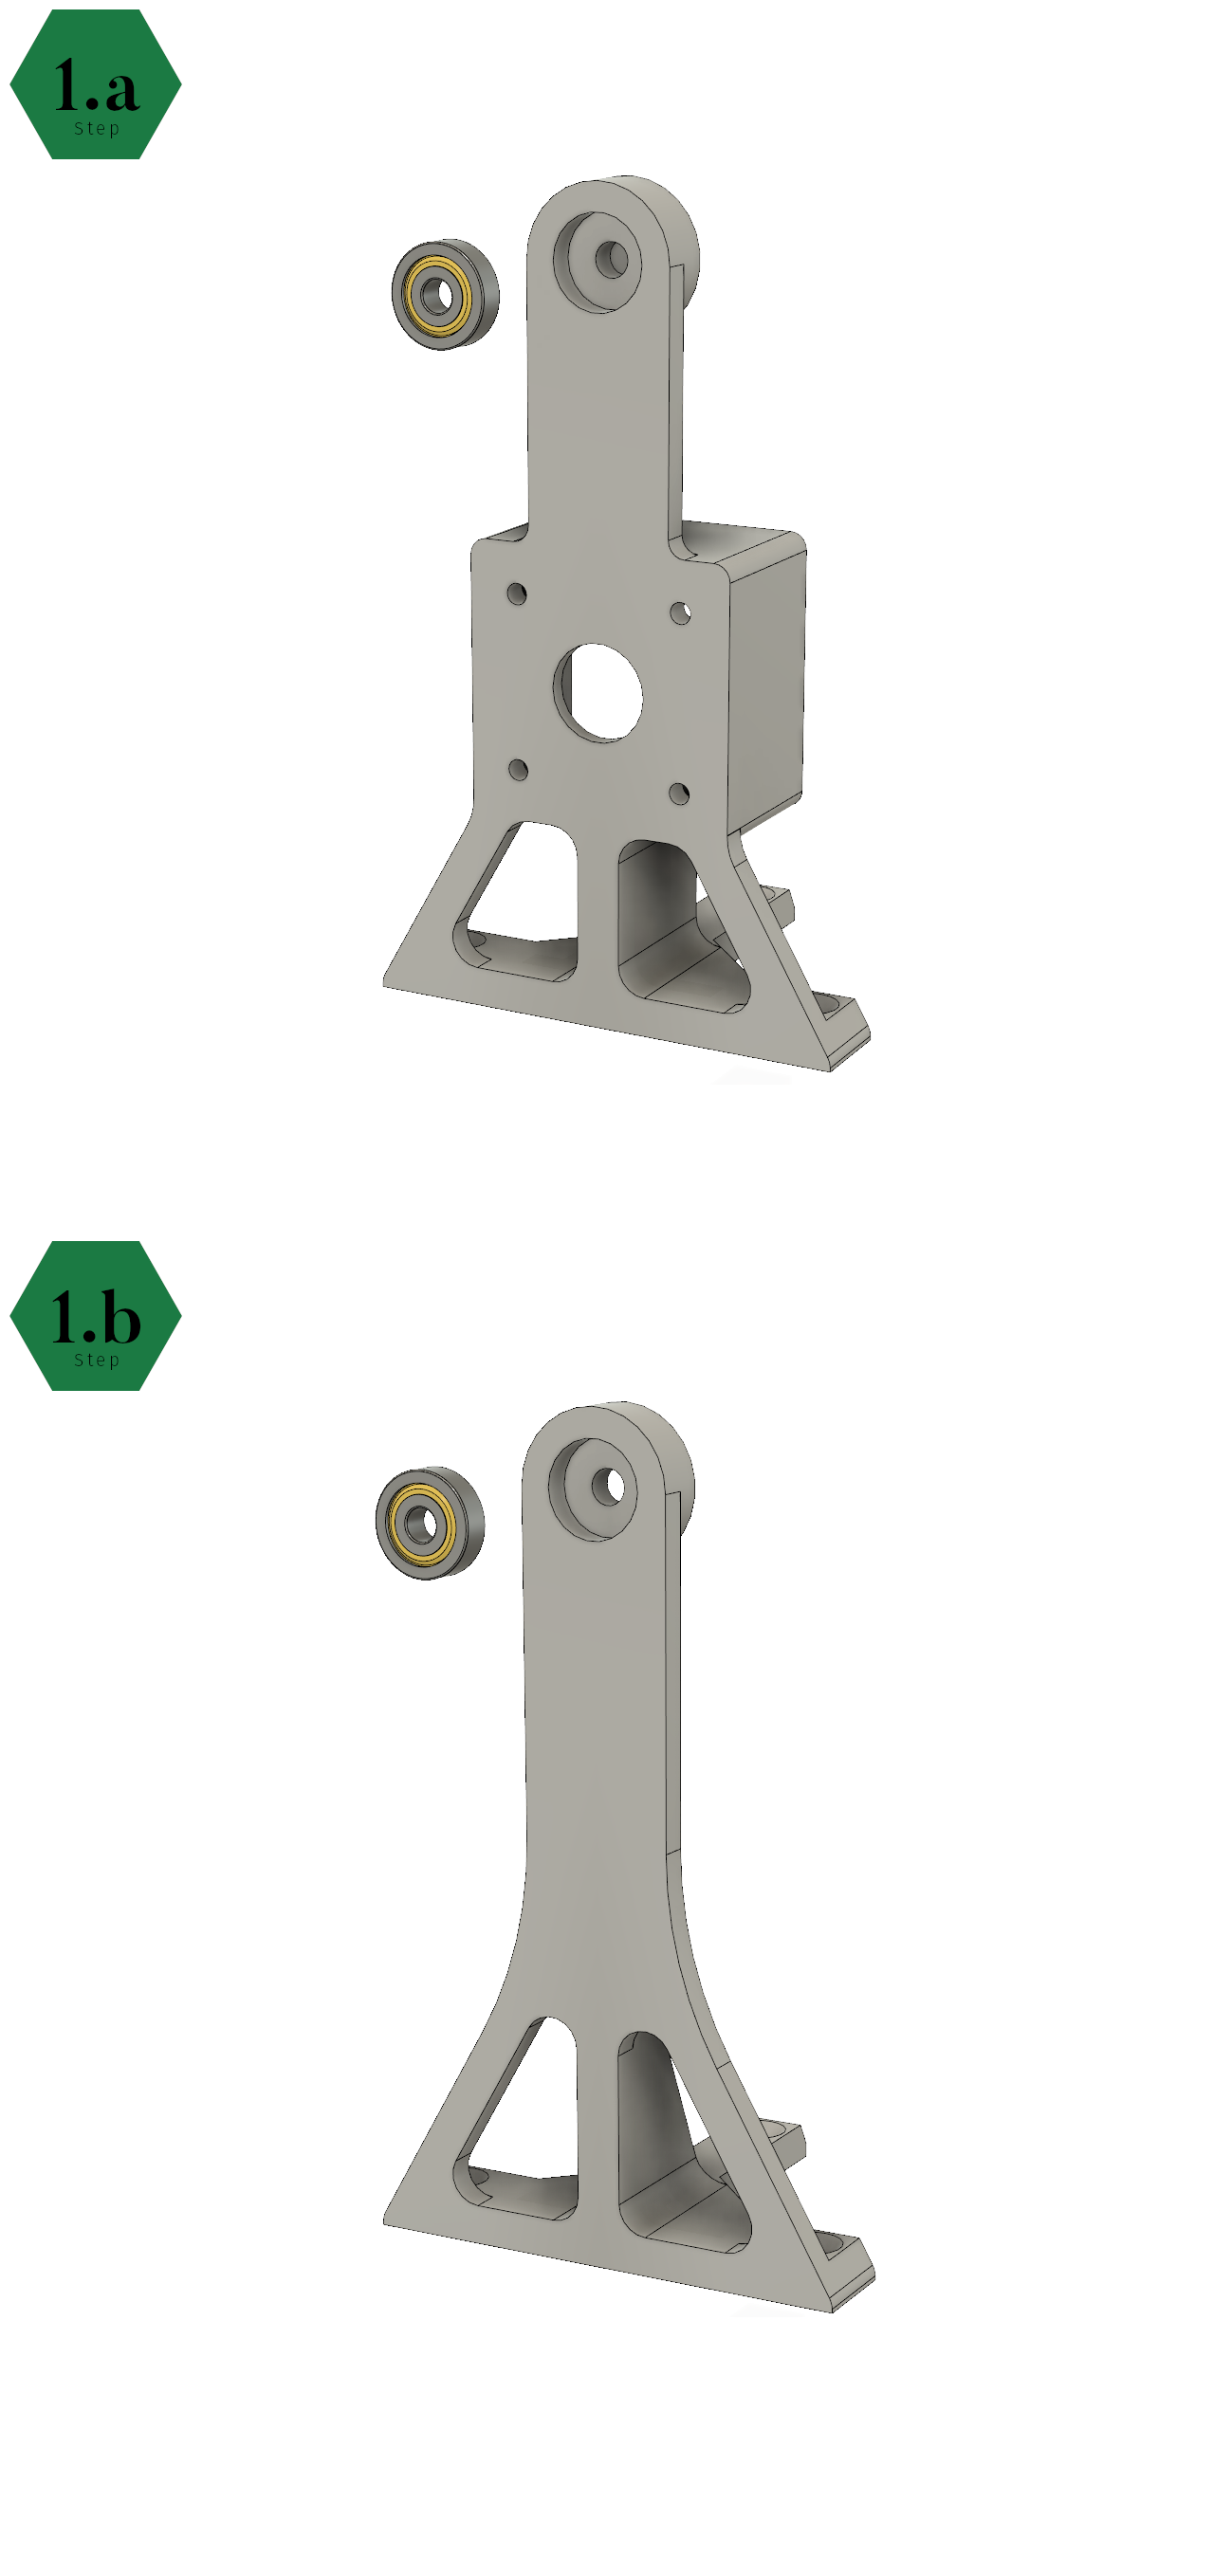
\includegraphics{images/Assembly1.png}%
{\captionof{figure}{Step 1 of the Open3DScanner assembly}}
\clearpage%

% STEP 2&3
\sideTabularx[Required parts for step 2]{%
	\rowcolors{2}{tableLineTwo}{tableLineOne}% specify rowcolors in tabularx style
	\begin{tabularx} {\marginparwidth} {>{\rowmac \hsize=1.5\hsize}X>{\rowmac \hsize=0.5\hsize}X<{\clearrow}}%
		\tabularxHeader%
		Part & Quantity\\%
		Nema 17 Stepper Motor & 2\\%
		Nema 17 Damper & 2\\%
		M3$\times$6 & 4\\%
	\end{tabularx}%
}%

\marginInfo*[Instructions]{Screw the dampers to the stepper motors.}%

\marginTips*[Tip]{The orientation of the dampers does not matter, it is only important that the side with the threads points away from the stepper motor.}%

\sideTabularx[Required parts for step 3]{%
	\vspace{2.65cm}%
	\rowcolors{2}{tableLineTwo}{tableLineOne}% specify rowcolors in tabularx style
	\begin{tabularx} {\marginparwidth} {>{\rowmac \hsize=1.5\hsize}X>{\rowmac \hsize=0.5\hsize}X<{\clearrow}}%
		\tabularxHeader%
		Part & Quantity\\%
		M3$\times$8 & 2\\%
	\end{tabularx}%
}%

\marginInfo*[Instructions]{Screw one stepper motor to the Rotor-Stand.}%

\marginCheck*[Check]{Make sure that the cables are pointing downwards to simplify the wiring later on.}%

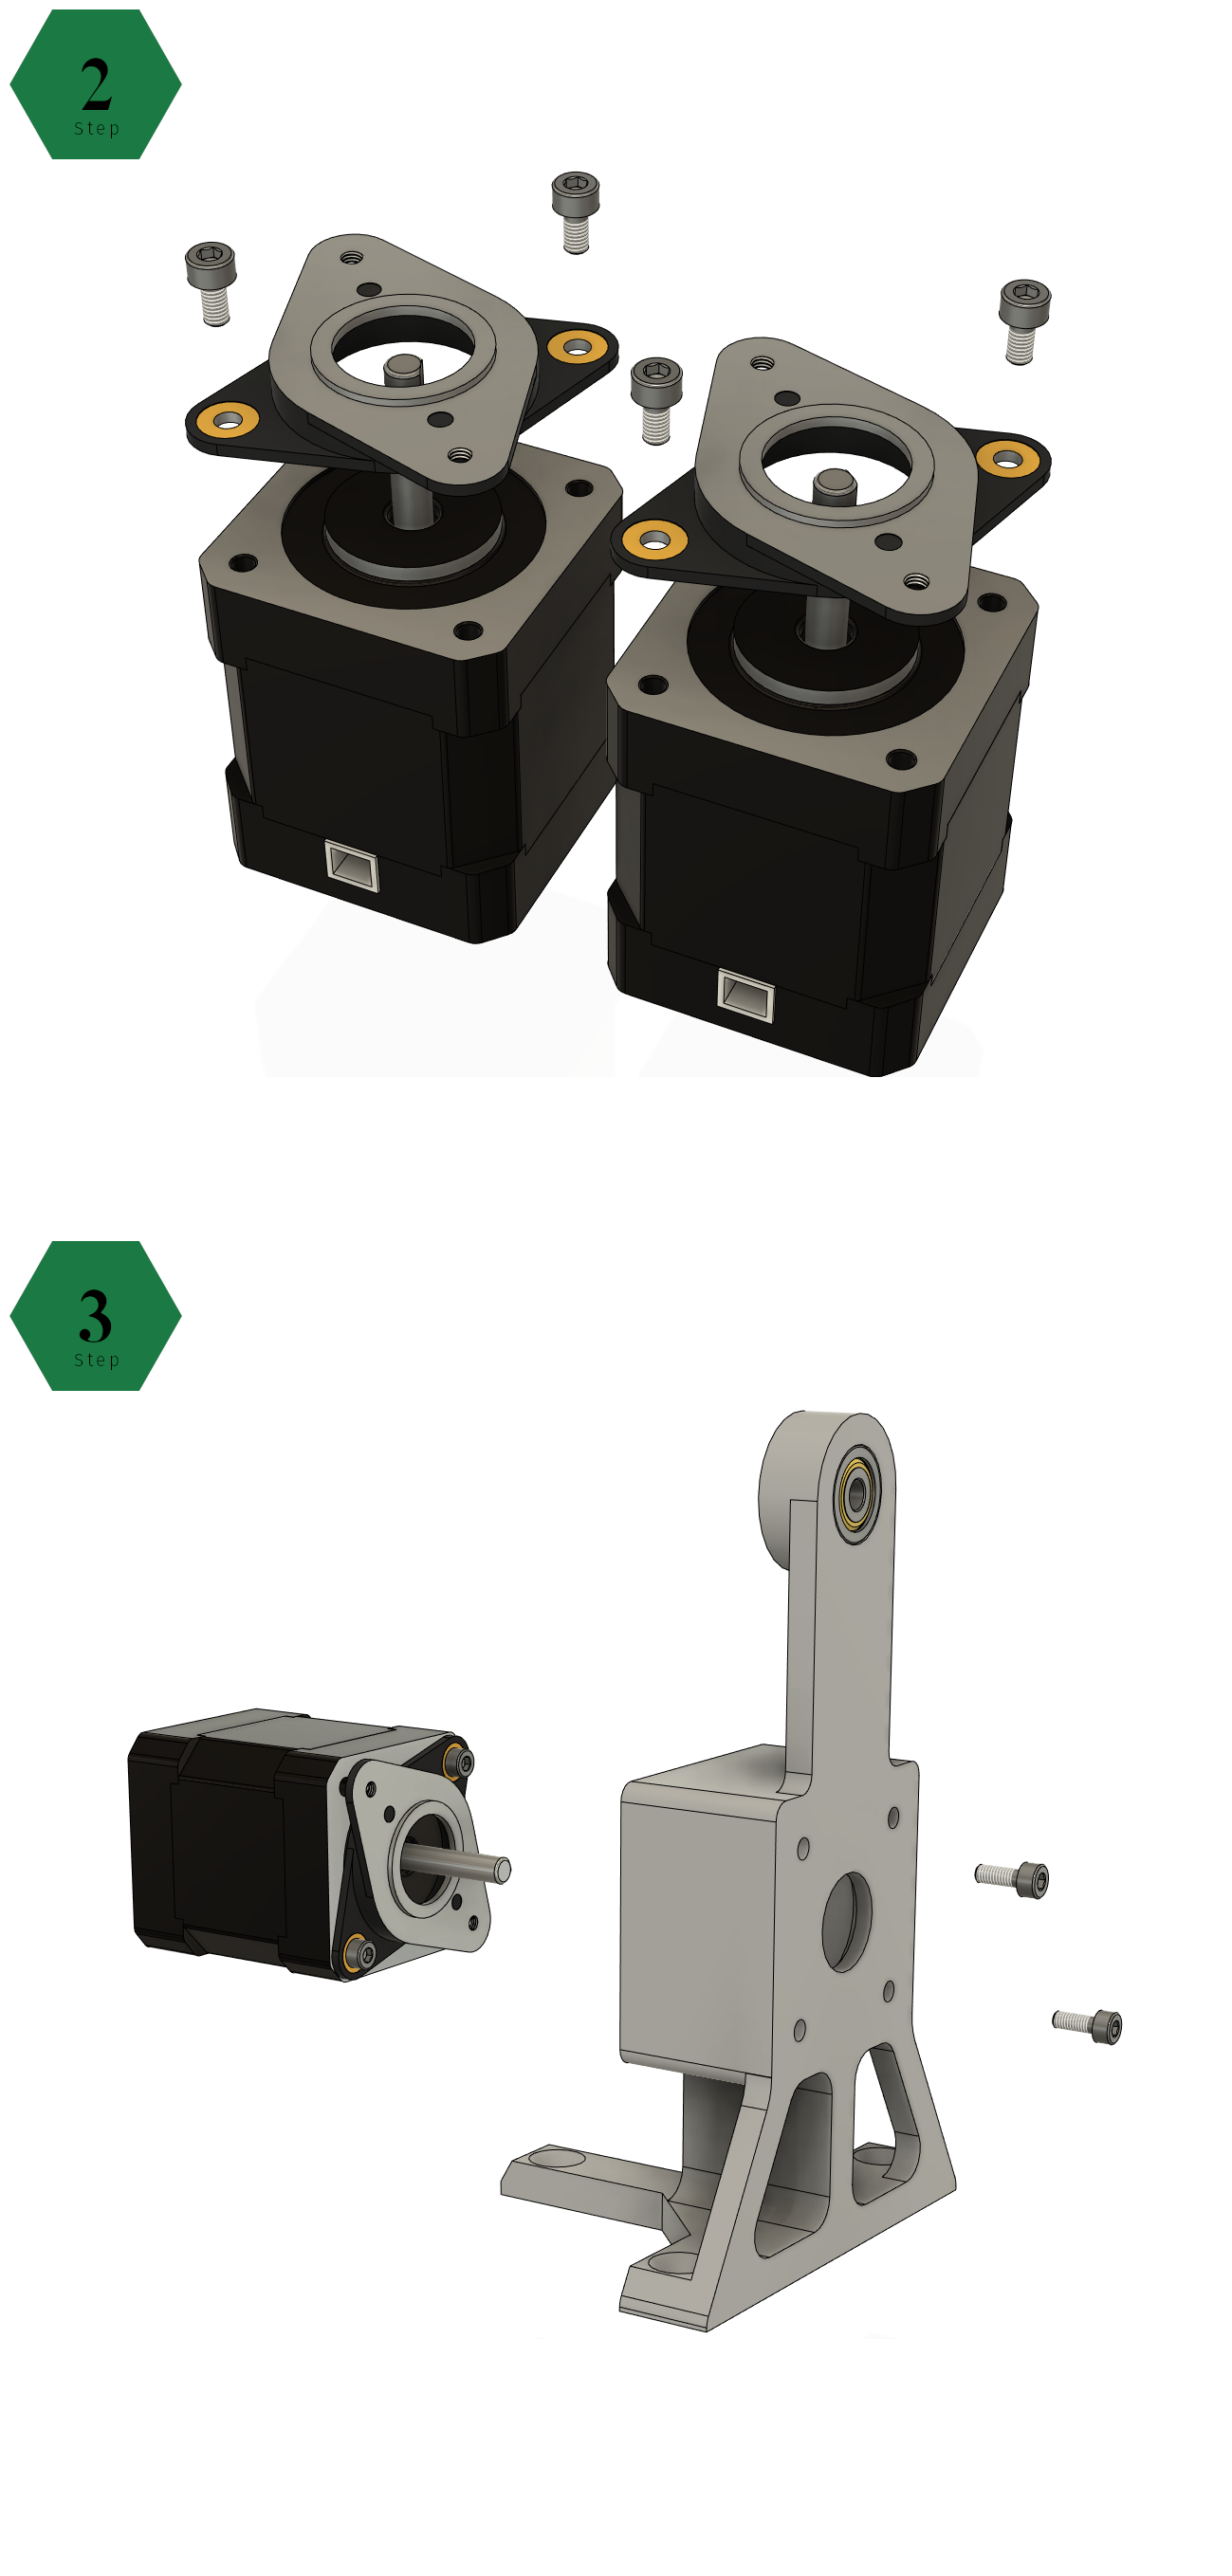
\includegraphics{images/Assembly2.png}%
{\captionof{figure}{Step 2 \& 3 of the Open3DScanner assembly}}
\clearpage%

% STEP 4
\sideTabularx[Required parts for step 4]{%
	\rowcolors{2}{tableLineTwo}{tableLineOne}% specify rowcolors in tabularx style
	\begin{tabularx} {\marginparwidth} {>{\rowmac \hsize=1.5\hsize}X>{\rowmac \hsize=0.5\hsize}X<{\clearrow}}%
		\tabularxHeader%
		Part & Quantity\\%
		Rotor-Gear & 1\\%
		Rotor-Pinion & 1\\%
		\SI{5}{\milli\meter} $\times$ \SI{26}{\milli\meter} Steel Rod & 1\\%
	\end{tabularx}%
}%

\marginInfo*[Instructions]{Press the Rotor-Pinion onto the shaft of the stepper motor. Press the steel rod into the bearing so that it is countersunk as far as possible in the printed part without hindering free rotation. Push the Rotor-Gear onto the steel rod. Use the middle hole of the Rotor-Gear for this.}%

\marginTips*[Tip]{The Rotor-Gear and the steel rod will not be flush. This is not problematic and improves the stability of the assembly in later steps.}%

\marginWarning*[Double check]{The design does not ensure alignment between the two gears. It is intended that the rotor gear is centered on the rotor pinion and protrudes about 1mm on both sides. This must be strictly adhered to in order to allow a smooth movement later on. The connections are so tight that the parts should not slip after alignment.}%

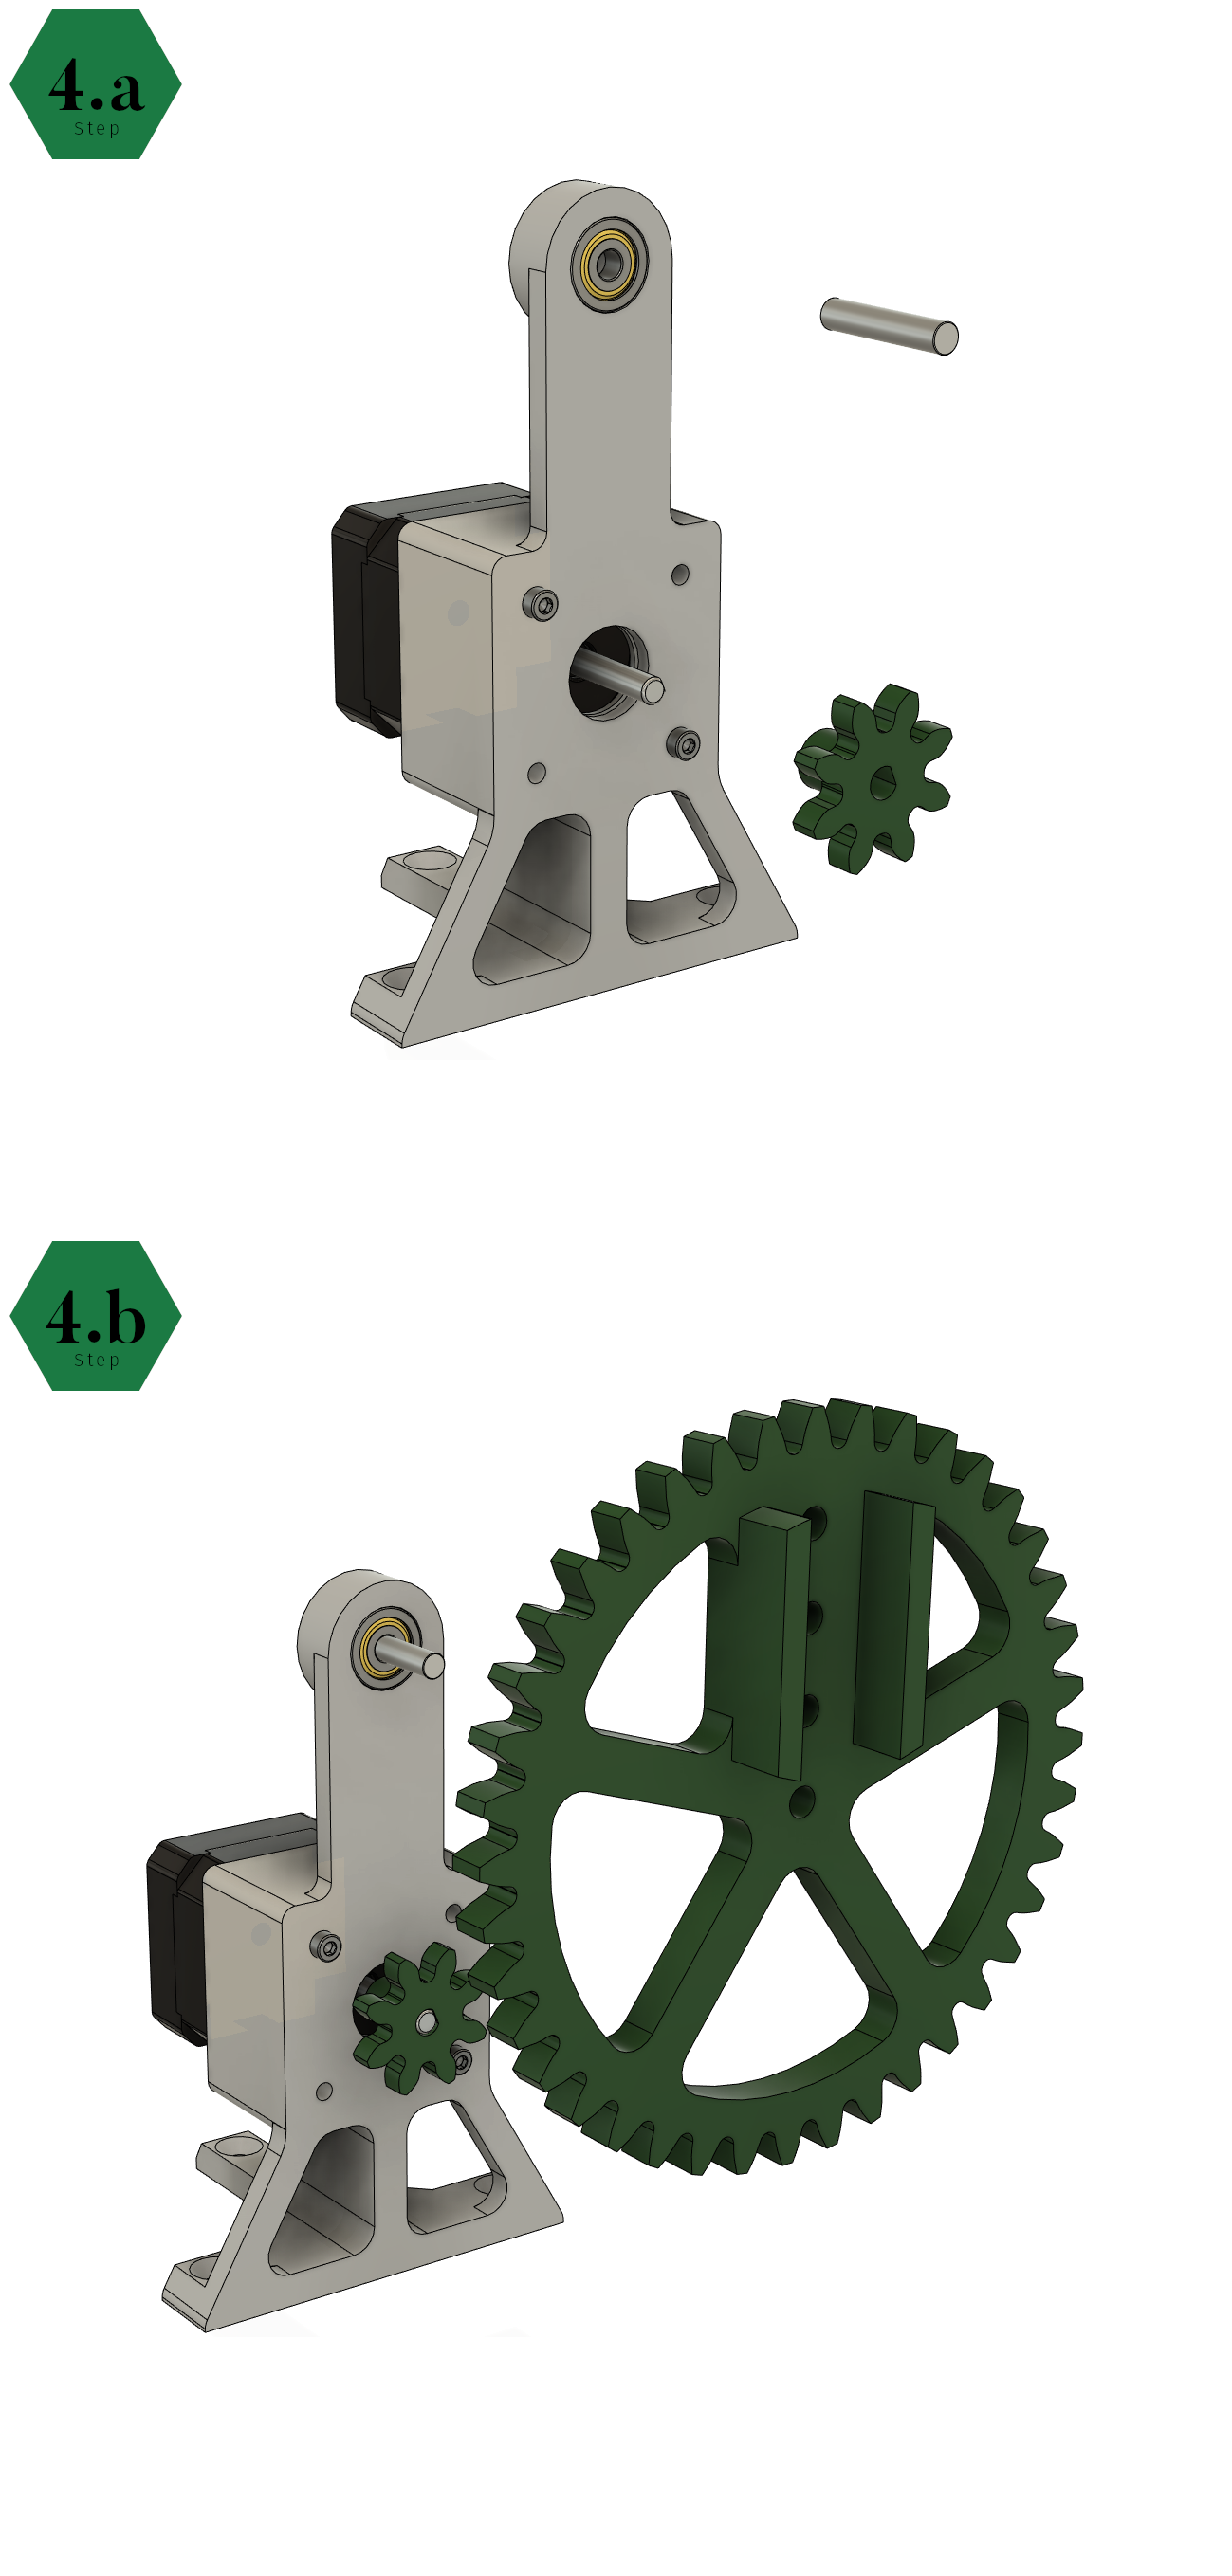
\includegraphics{images/Assembly3.png}%
{\captionof{figure}{Step 4 of the Open3DScanner assembly}}
\clearpage%

% STEP 5
\sideTabularx[Required parts for step 5]{%
	\rowcolors{2}{tableLineTwo}{tableLineOne}% specify rowcolors in tabularx style
	\begin{tabularx} {\marginparwidth} {>{\rowmac \hsize=1.5\hsize}X>{\rowmac \hsize=0.5\hsize}X<{\clearrow}}%
		\tabularxHeader%
		Part & Quantity\\%
		Rotor-Arm & 2\\%
		Turntable-Arm & 1\\%
		\SI{5}{\milli\meter} $\times$ \SI{26}{\milli\meter} Steel Rod & 2\\%
	\end{tabularx}%
}%

\marginInfo*[Instructions]{Press one Rotor-Arm on each end of the Turntable-Arm so that they are flush with the holes. Press a steel rod into each of the holes to firmly join the components together. The steel rods should be flush with the Rotor-Arm on both sides.}%

\marginCheck*[Check]{Make sure that the Turntable-Arm is correctly turned to prevent subsequent disassembly and correction.}%

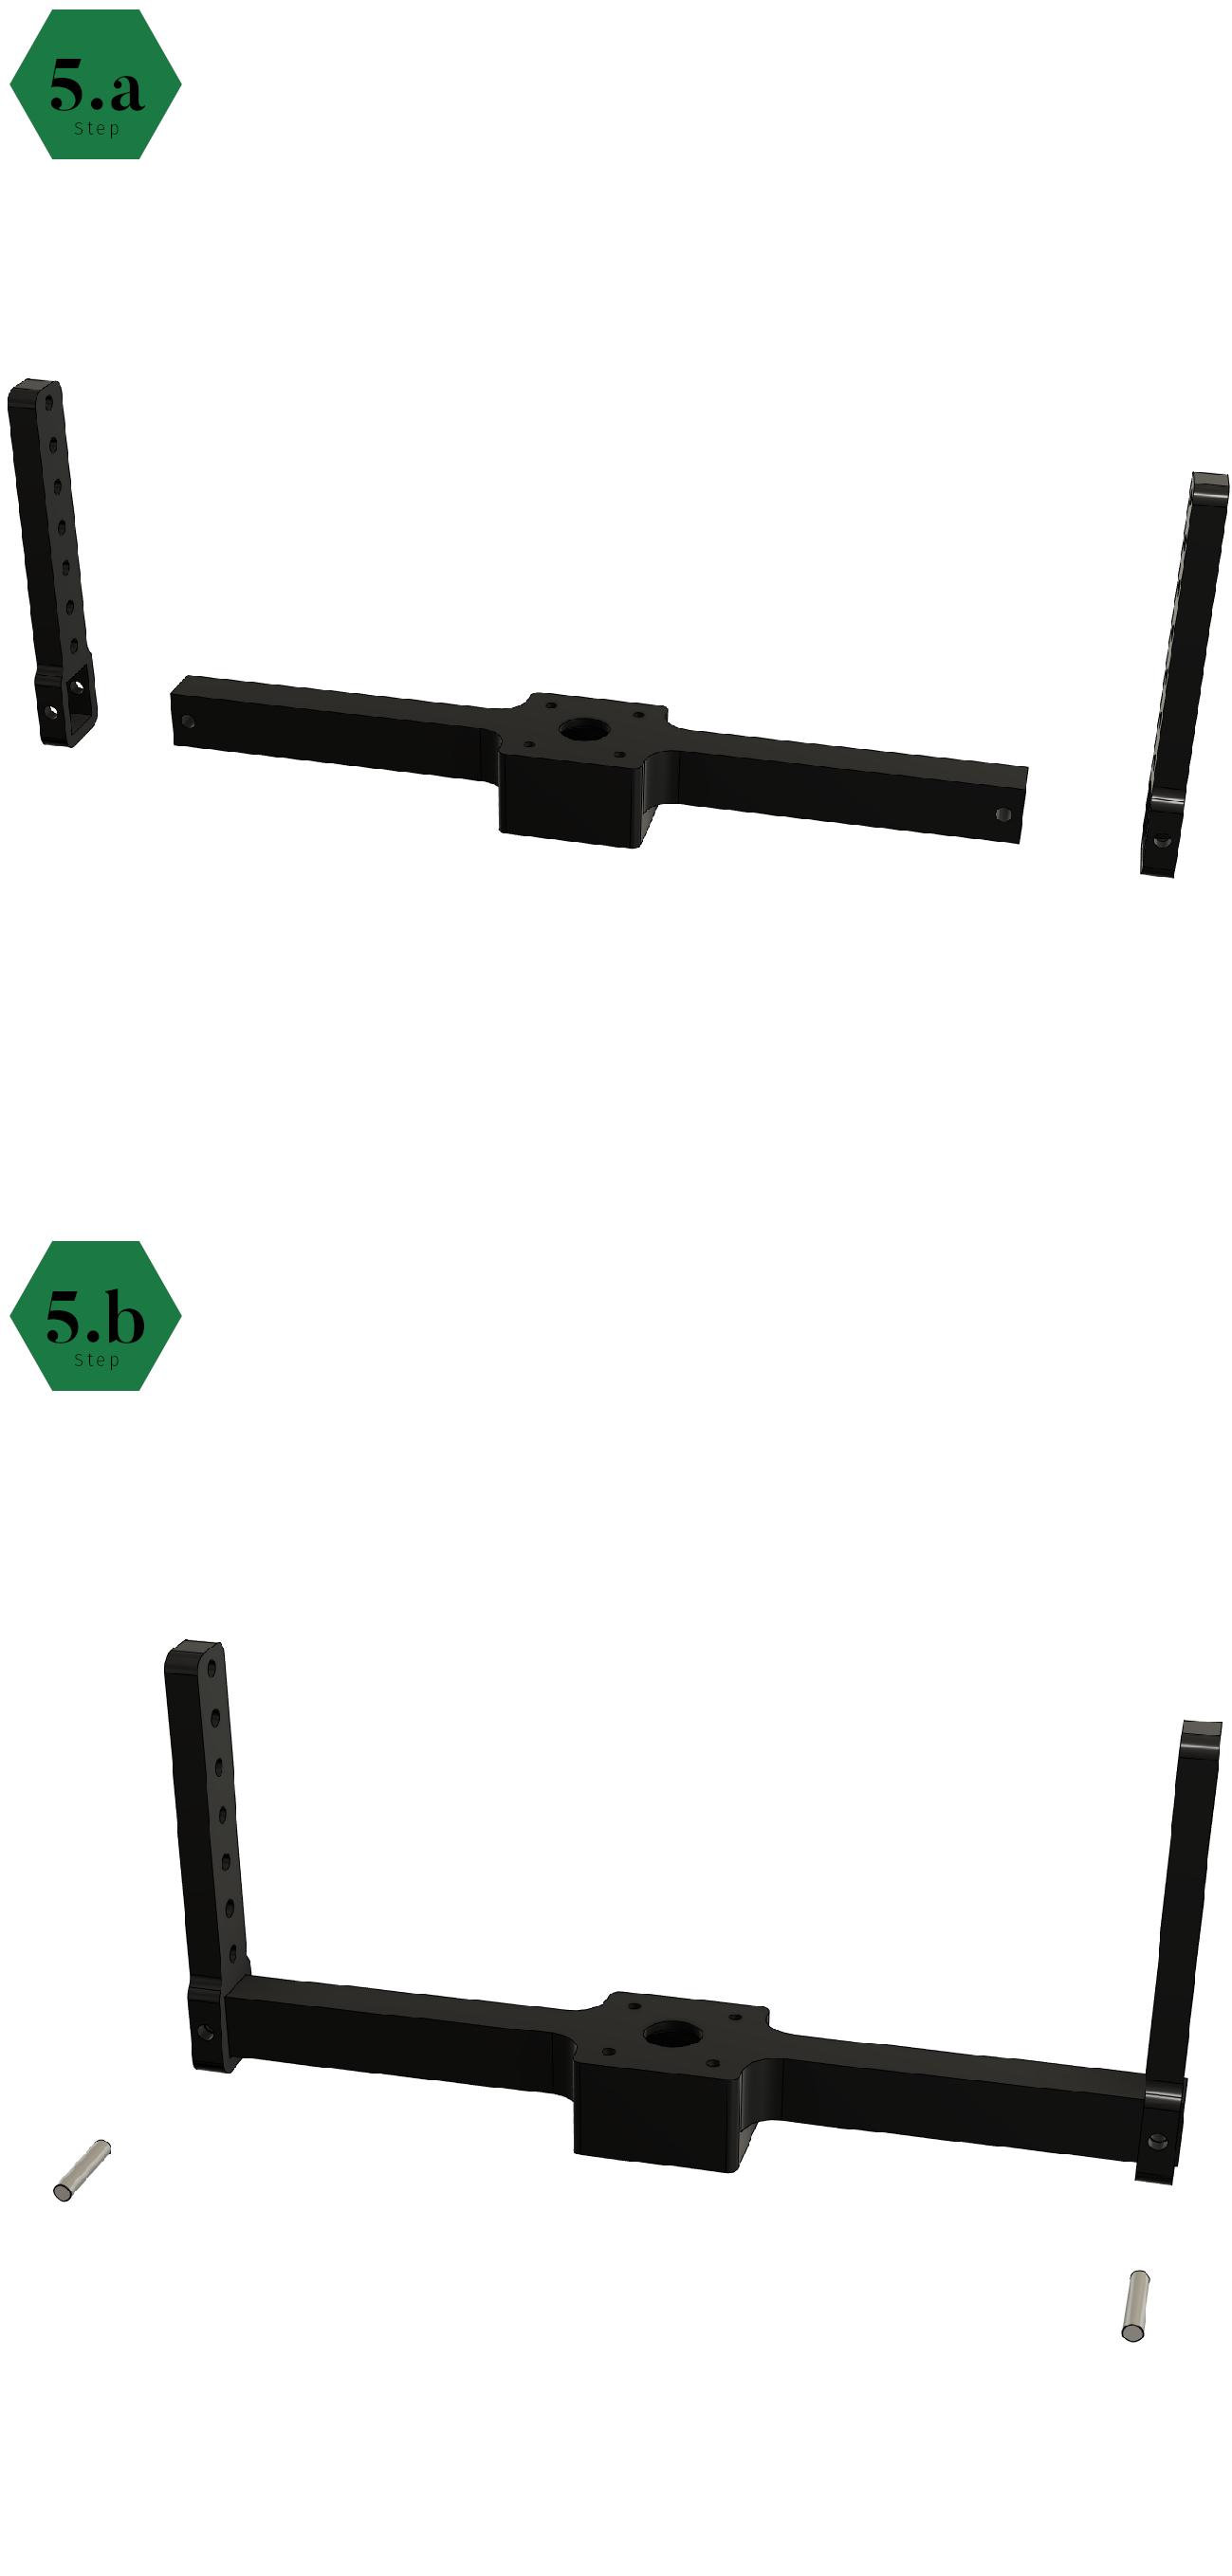
\includegraphics{images/Assembly4.png}%
{\captionof{figure}{Step 5 of the Open3DScanner assembly}}
\clearpage%

% STEP 6 & 7
\sideTabularx[Required parts for step 6]{%
	\rowcolors{2}{tableLineTwo}{tableLineOne}% specify rowcolors in tabularx style
	\begin{tabularx} {\marginparwidth} {>{\rowmac \hsize=1.5\hsize}X>{\rowmac \hsize=0.5\hsize}X<{\clearrow}}%
		\tabularxHeader%
		Part & Quantity\\%
		M3$\times$8 & 2\\%
	\end{tabularx}%
}%

\marginInfo*[Instructions]{Screw the remaining stepper motor to the Turntable-Arm.}%

\sideTabularx[Required parts for step 7]{%
	\vspace{5.7cm}%
	\rowcolors{2}{tableLineTwo}{tableLineOne}% specify rowcolors in tabularx style
	\begin{tabularx} {\marginparwidth} {>{\rowmac \hsize=1.5\hsize}X>{\rowmac \hsize=0.5\hsize}X<{\clearrow}}%
		\tabularxHeader%
		Part & Quantity\\%
		\SI{5}{\milli\meter} $\times$ \SI{26}{\milli\meter} Steel Rod & 1\\%
	\end{tabularx}%
}%

\marginInfo*[Instructions]{Push the steel rod through the upper hole of one Rotor-Arm and then into the outer hole of the Rotor-Gear. The components should be flush with each other and the Rotor-Arm is fixed to the rotor gear by the two jaws.}%

\marginQuestion*[Information]{The Rotor-Arm is additionally fixed by the steel rod, which connects the Rotor-Gear with the Rotor-Stand.}%

\marginCheck*[Check]{Make sure that the motor cables point towards you when the Rotor-Stand is on the left side. This will allow clean wiring.}%

\marginCritical*[Warning]{For accurate alignment of the steel bar, consider the image cutout. The rod must protrude a little bit from the rotor arm, otherwise the rotation of the device will be blocked.}%

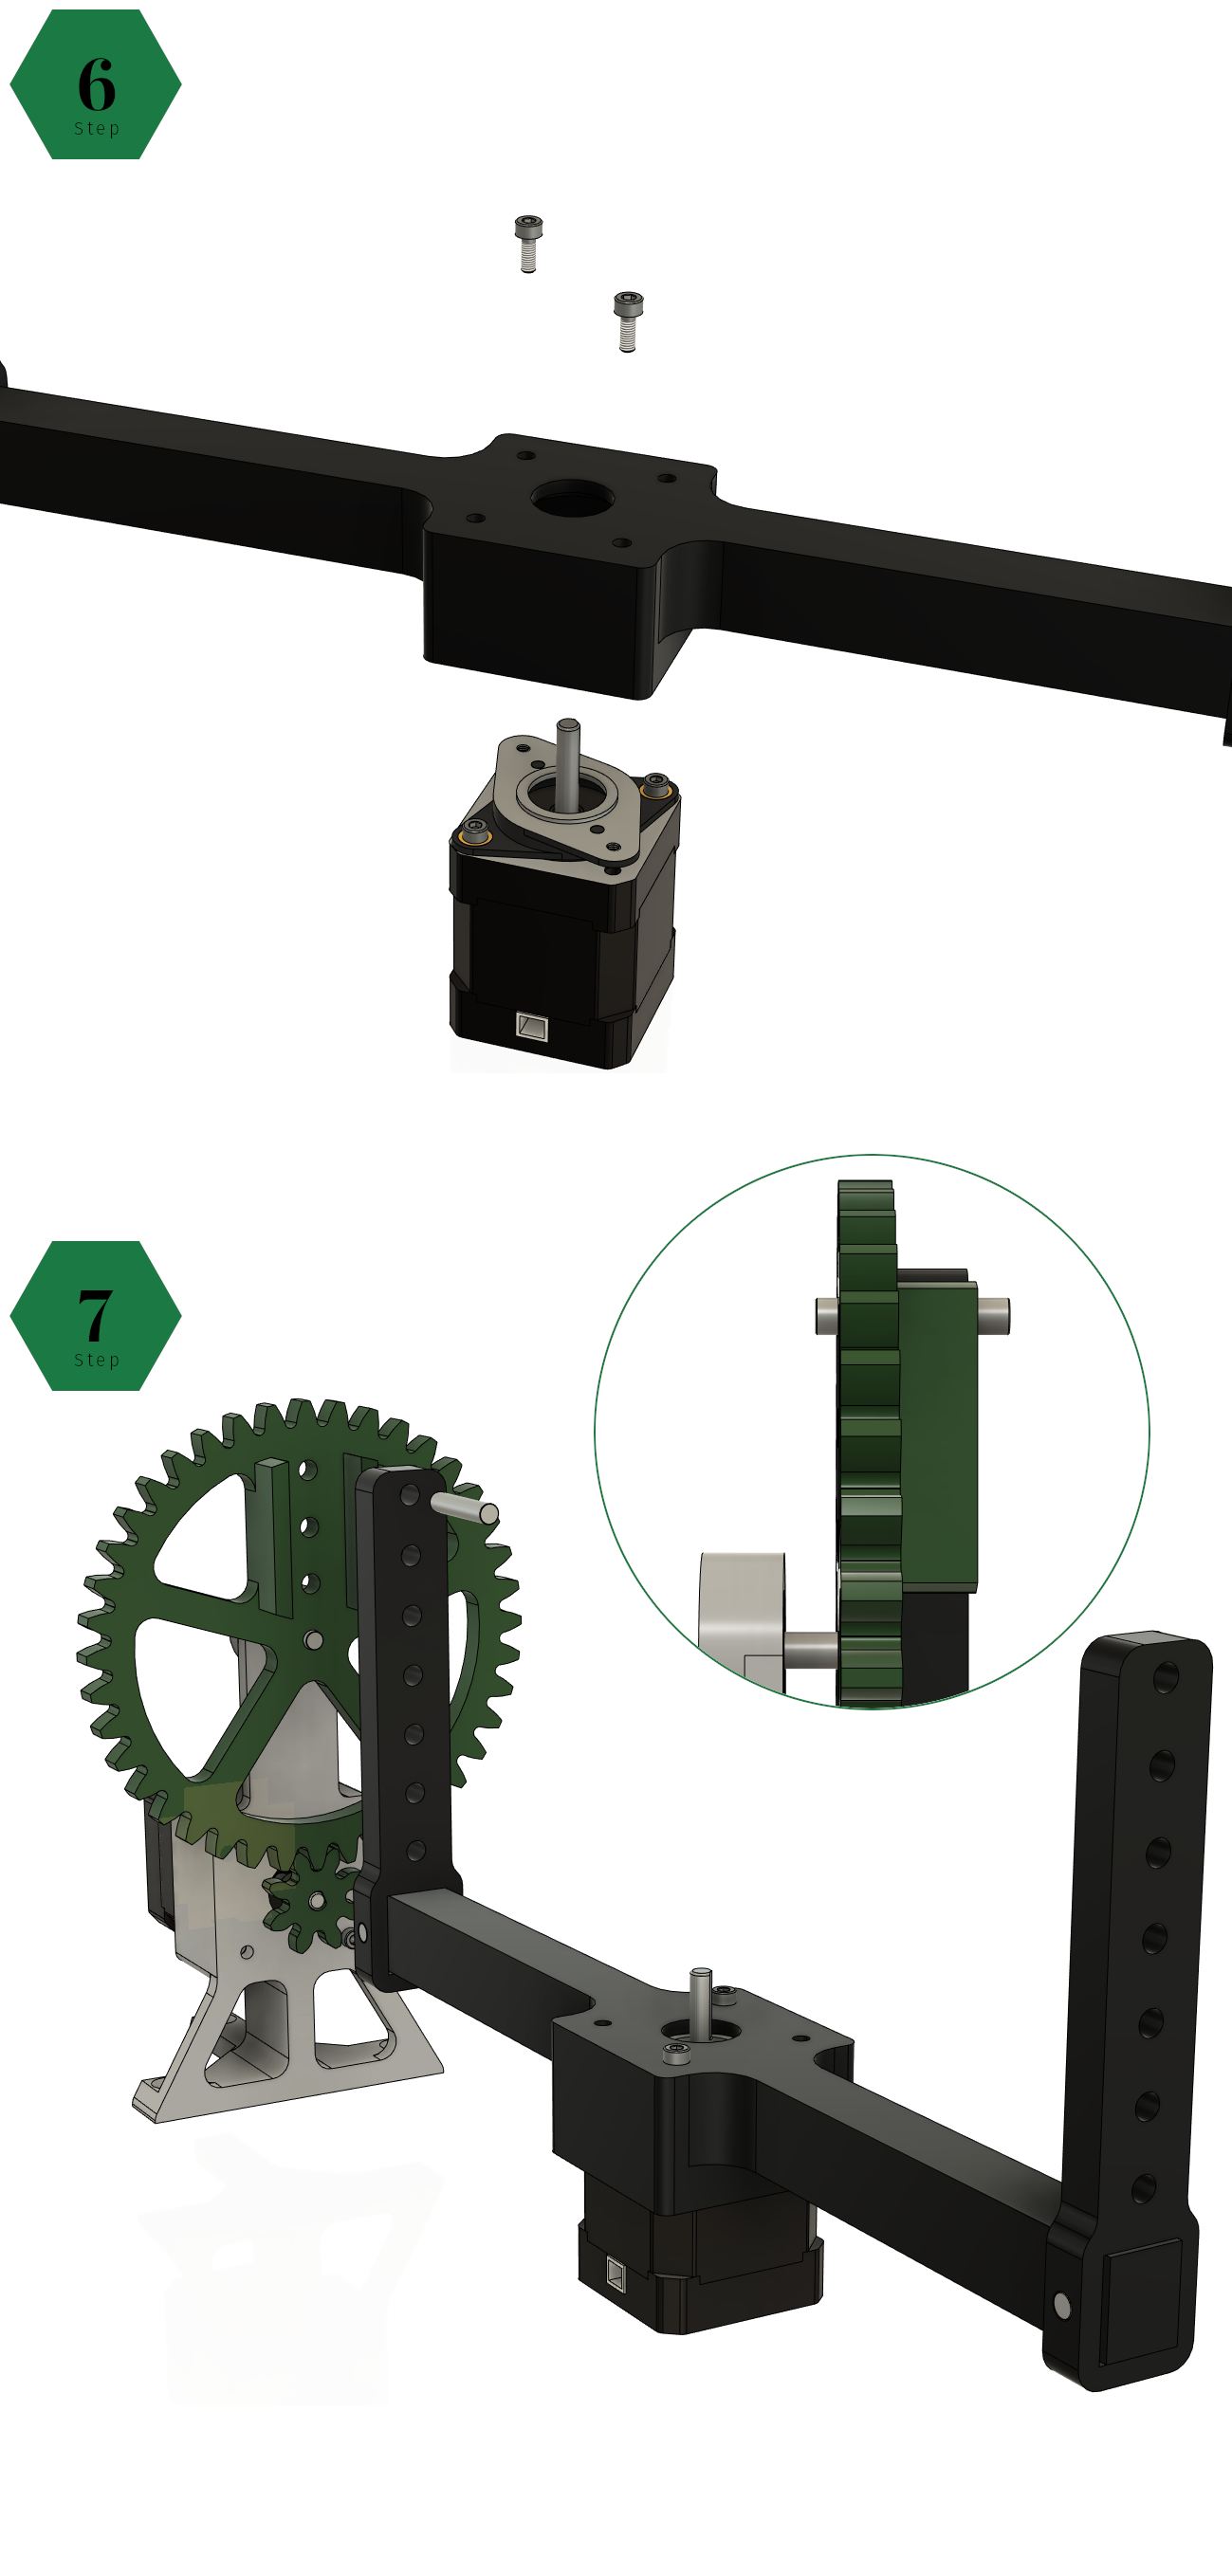
\includegraphics{images/Assembly5.png}%
{\captionof{figure}{Step 6 \& 7 of the Open3DScanner assembly}}
\clearpage%

% STEP 8 & 9
\sideTabularx[Required parts for step 8]{%
	\rowcolors{2}{tableLineTwo}{tableLineOne}% specify rowcolors in tabularx style
	\begin{tabularx} {\marginparwidth} {>{\rowmac \hsize=1.5\hsize}X>{\rowmac \hsize=0.5\hsize}X<{\clearrow}}%
		\tabularxHeader%
		Part & Quantity\\%
		\SI{5}{\milli\meter} $\times$ \SI{26}{\milli\meter} Steel Rod & 1\\%
	\end{tabularx}%
}%

\marginInfo*[Instructions]{Connect the other Rotor-Arm to the bearing in the Passive-Stand. Use the center hole in the Rotor-Arm for this. The rod will be flush with the Rotor-Arm and protrude a bit from the back of the Passive-Stand.}%

\sideTabularx[Required parts for step 9]{%
	\vspace{5.0cm}%
	\rowcolors{2}{tableLineTwo}{tableLineOne}% specify rowcolors in tabularx style
	\begin{tabularx} {\marginparwidth} {>{\rowmac \hsize=1.5\hsize}X>{\rowmac \hsize=0.5\hsize}X<{\clearrow}}%
		\tabularxHeader%
		Part & Quantity\\%
		Turntable-Medium & 1\\%
	\end{tabularx}%
}%

\marginInfo*[Instructions]{Push the Turntable-Medium as far as possible onto the shaft of the stepper motor, which is mounted to the Turntable-Arm.}%

\marginTips*[Tip]{Stabilize the structure by pressing against the bottom of the Turntable-Arm while pushing the Turntable-Medium onto the motor shaft. That way bending and deformation of the parts can be prevented.}%

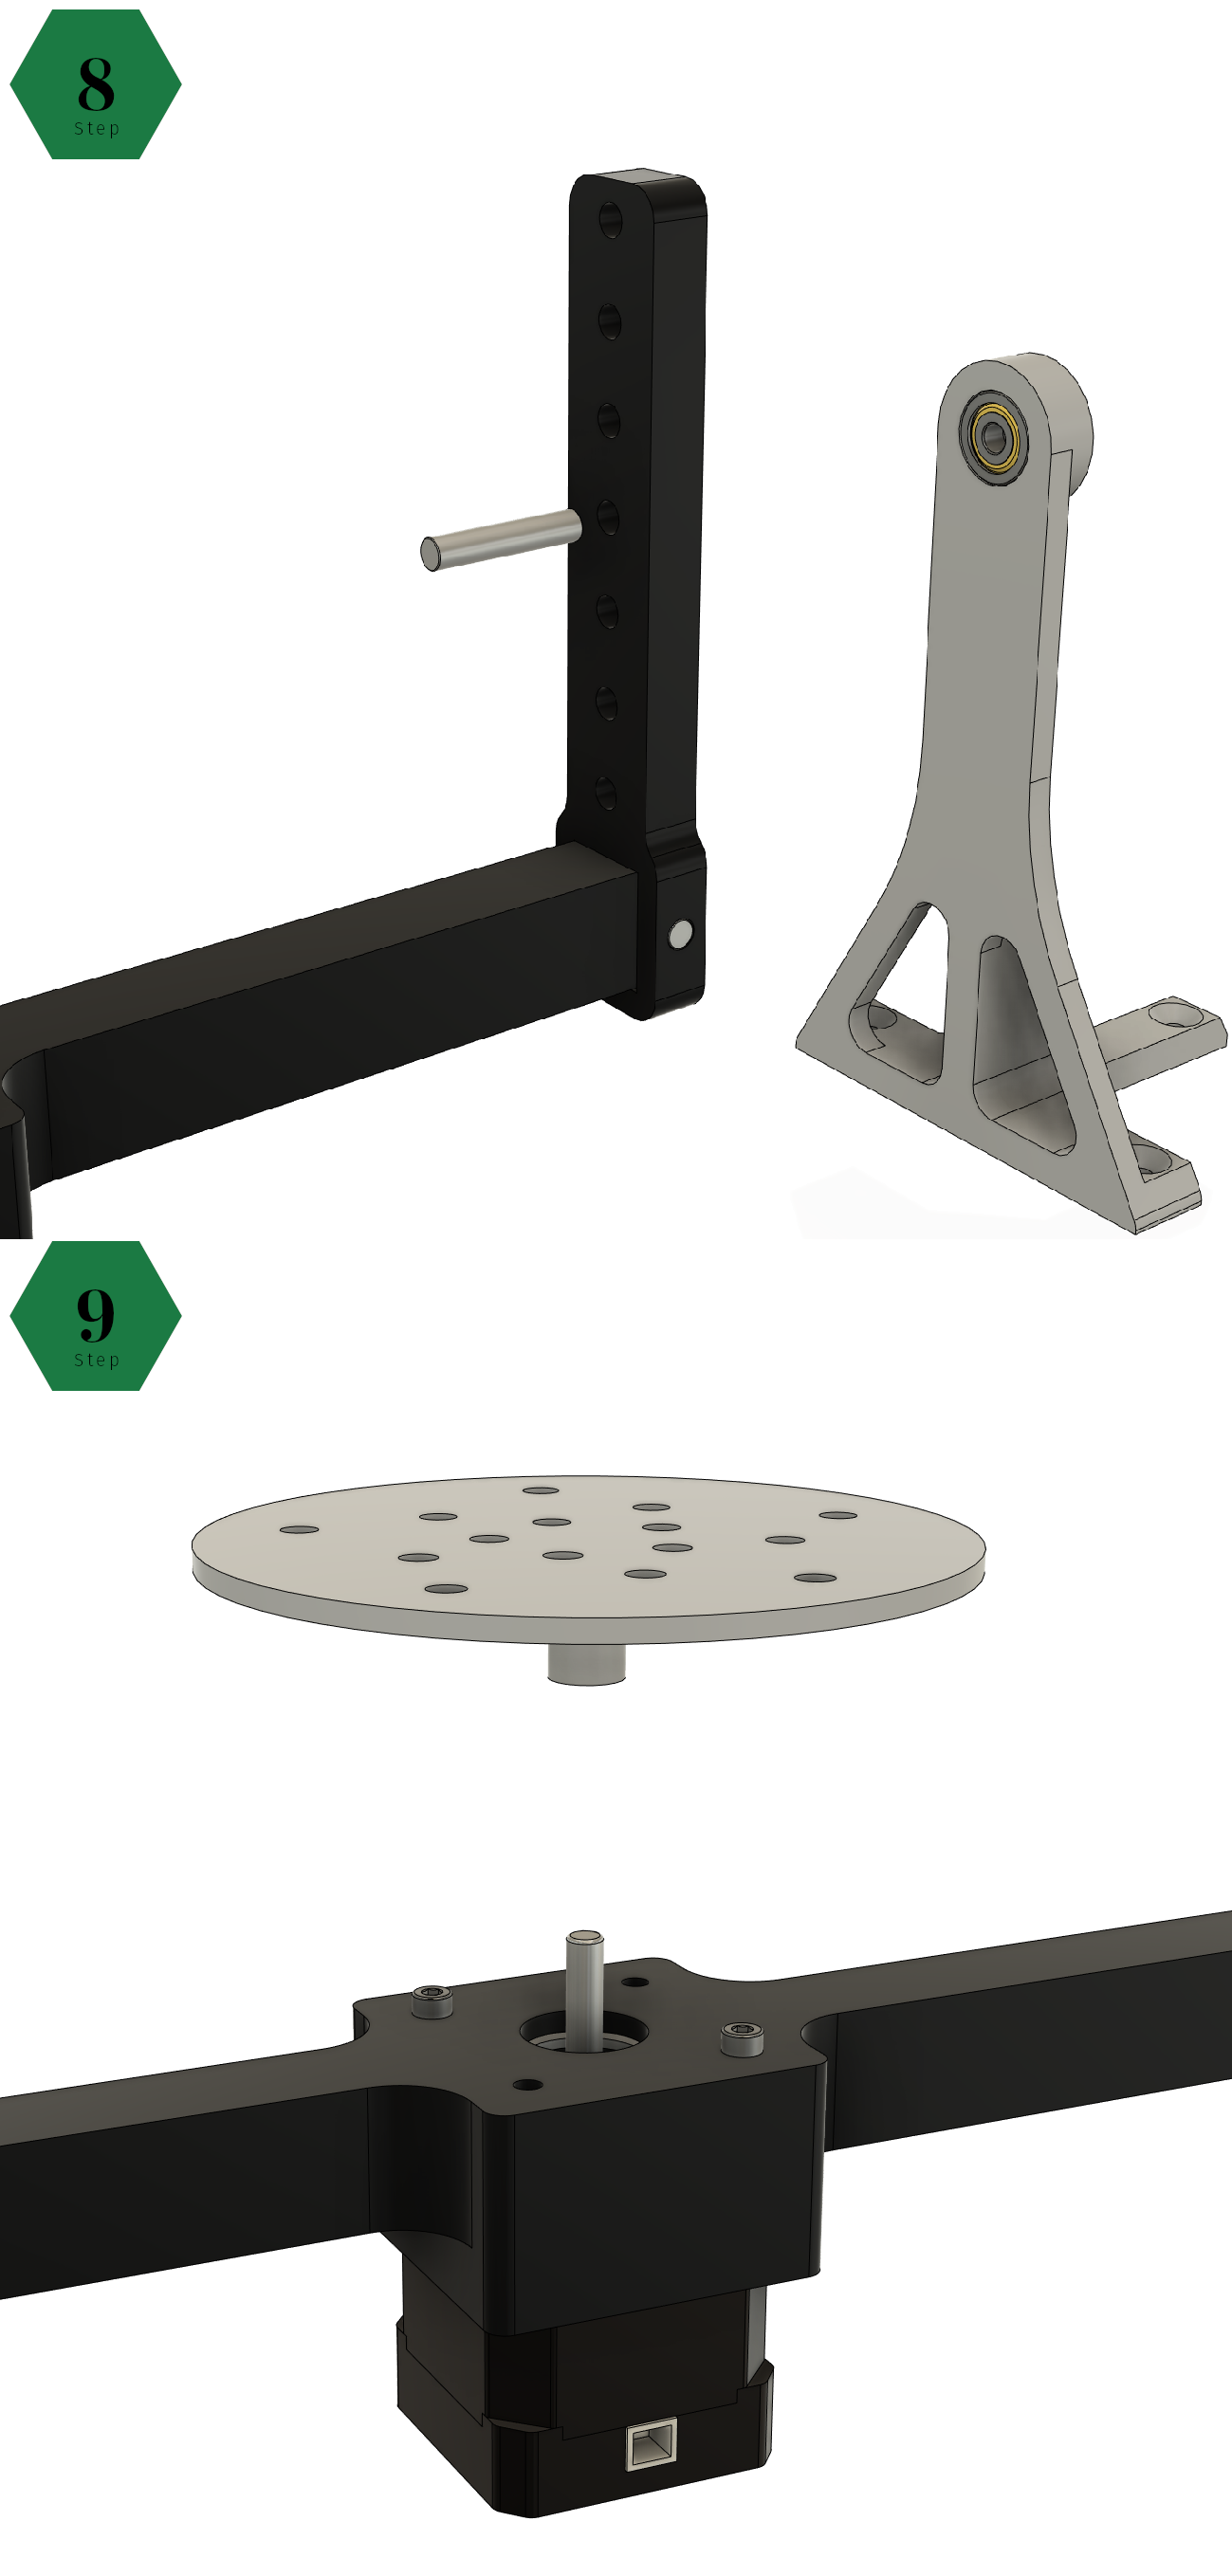
\includegraphics{images/Assembly6.png}%
{\captionof{figure}{Step 8 \& 9 of the Open3DScanner assembly}}
\clearpage%

% STEP 10
\sideTabularx[Required parts for step 10]{%
	\rowcolors{2}{tableLineTwo}{tableLineOne}% specify rowcolors in tabularx style
	\begin{tabularx} {\marginparwidth} {>{\rowmac \hsize=1.5\hsize}X>{\rowmac \hsize=0.5\hsize}X<{\clearrow}}%
		\tabularxHeader%
		Part & Quantity\\%
		Spotlight-Stand & 1\\%
		Spotlight-Frame & 1\\%
		M3$\times$8 & 2\\%
		M3 Nut & 2\\%
	\end{tabularx}%
}%

\marginInfo*[Instructions]{Press the two nuts into the recesses of the Spotlight-Stand. Select two adjacent holes that are at the same height. Next attach the Spotlight-Frame with the Spotlight-Stand. To do this, screw the screws through the holes in the Spotlight-Frame with the nuts on the back of the Spotlight-Stand.}%

\marginTips*[Tip]{Repeat this step up to four times for each spotlight you want to use. The height of the Spotlight frame can be changed by inserting the nuts into other recesses. This allows the illumination for the scans to be changed. The hole in the middle of the lower part of the Spotlight-Frame is for cable routing.}%

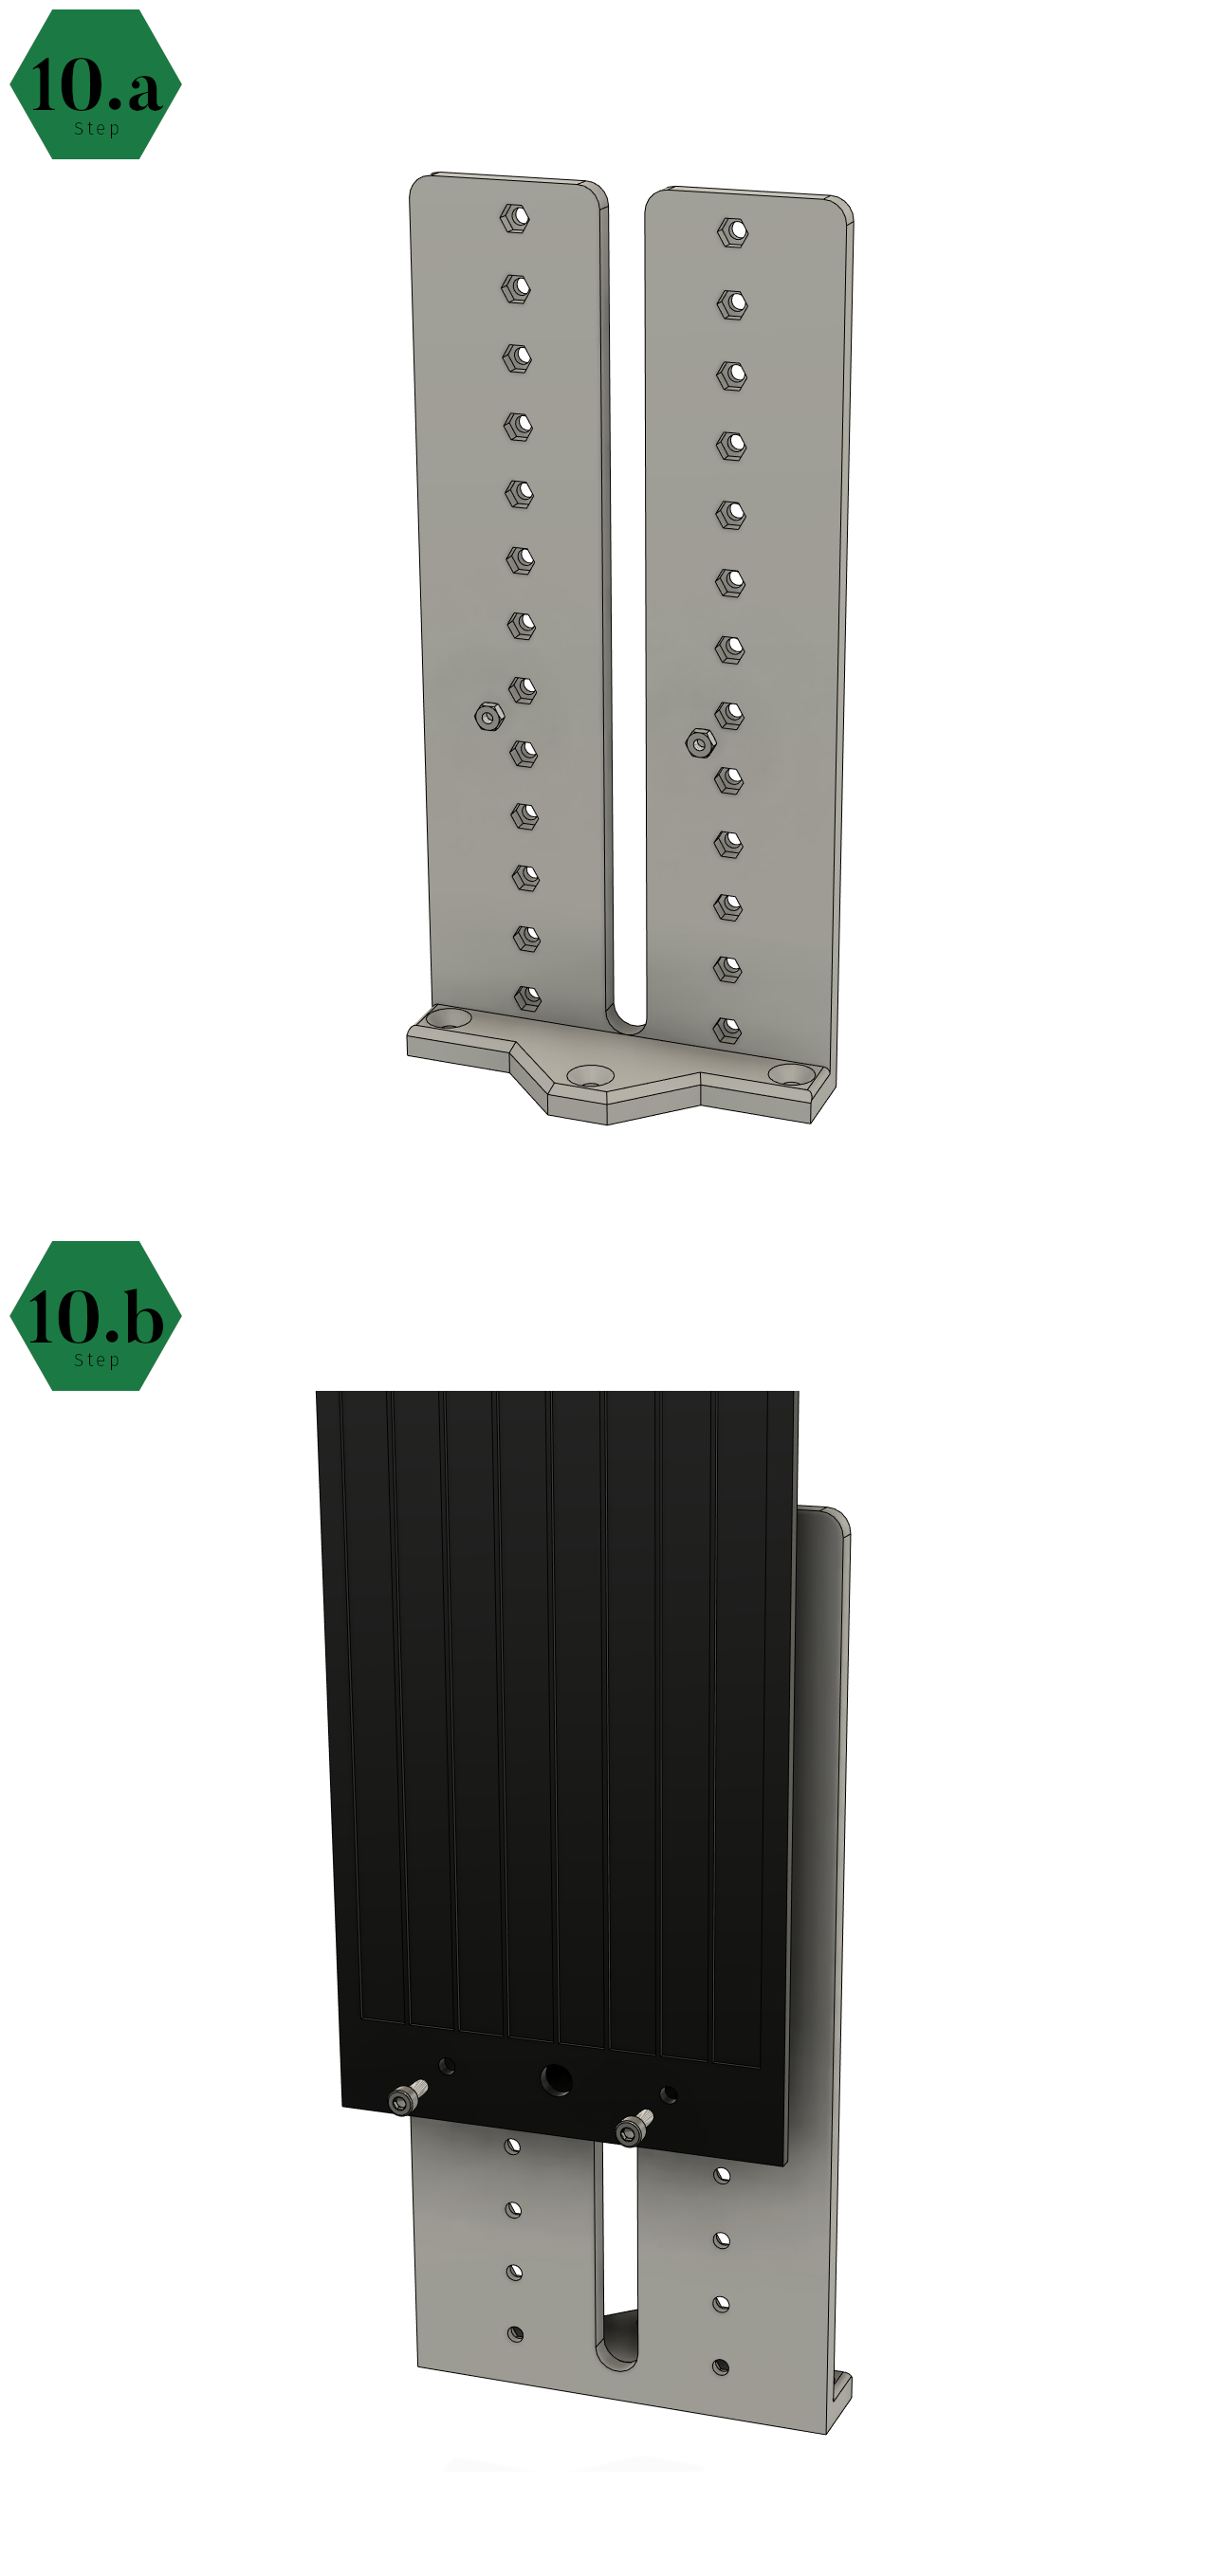
\includegraphics{images/Assembly7.png}%
{\captionof{figure}{Step 10 of the Open3DScanner assembly}}
\clearpage%

% STEP 11
\sideTabularx[Required parts for step 11]{%
	\rowcolors{2}{tableLineTwo}{tableLineOne}% specify rowcolors in tabularx style
	\begin{tabularx} {\marginparwidth} {>{\rowmac \hsize=1.5\hsize}X>{\rowmac \hsize=0.5\hsize}X<{\clearrow}}%
		\tabularxHeader%
		Part & Quantity\\%
		Foot-Holder-Clamp & 4\\%
		\SI{30}{\milli\meter} $\times$ \SI{15}{\milli\meter} Rubber Feet & 4\\%
		M3$\times$20 & 4\\%
		M3 Nut & 4\\%
	\end{tabularx}%
}%

\marginInfo*[Instructions]{Press the nut into the recess on top of the Foot-Holder-Clamp. Then screw the rubber feet with the screw from the bottom to the nut.}%

\marginTips*[Tip]{Repeat this step four times to assemble all feet for the base plate.}%

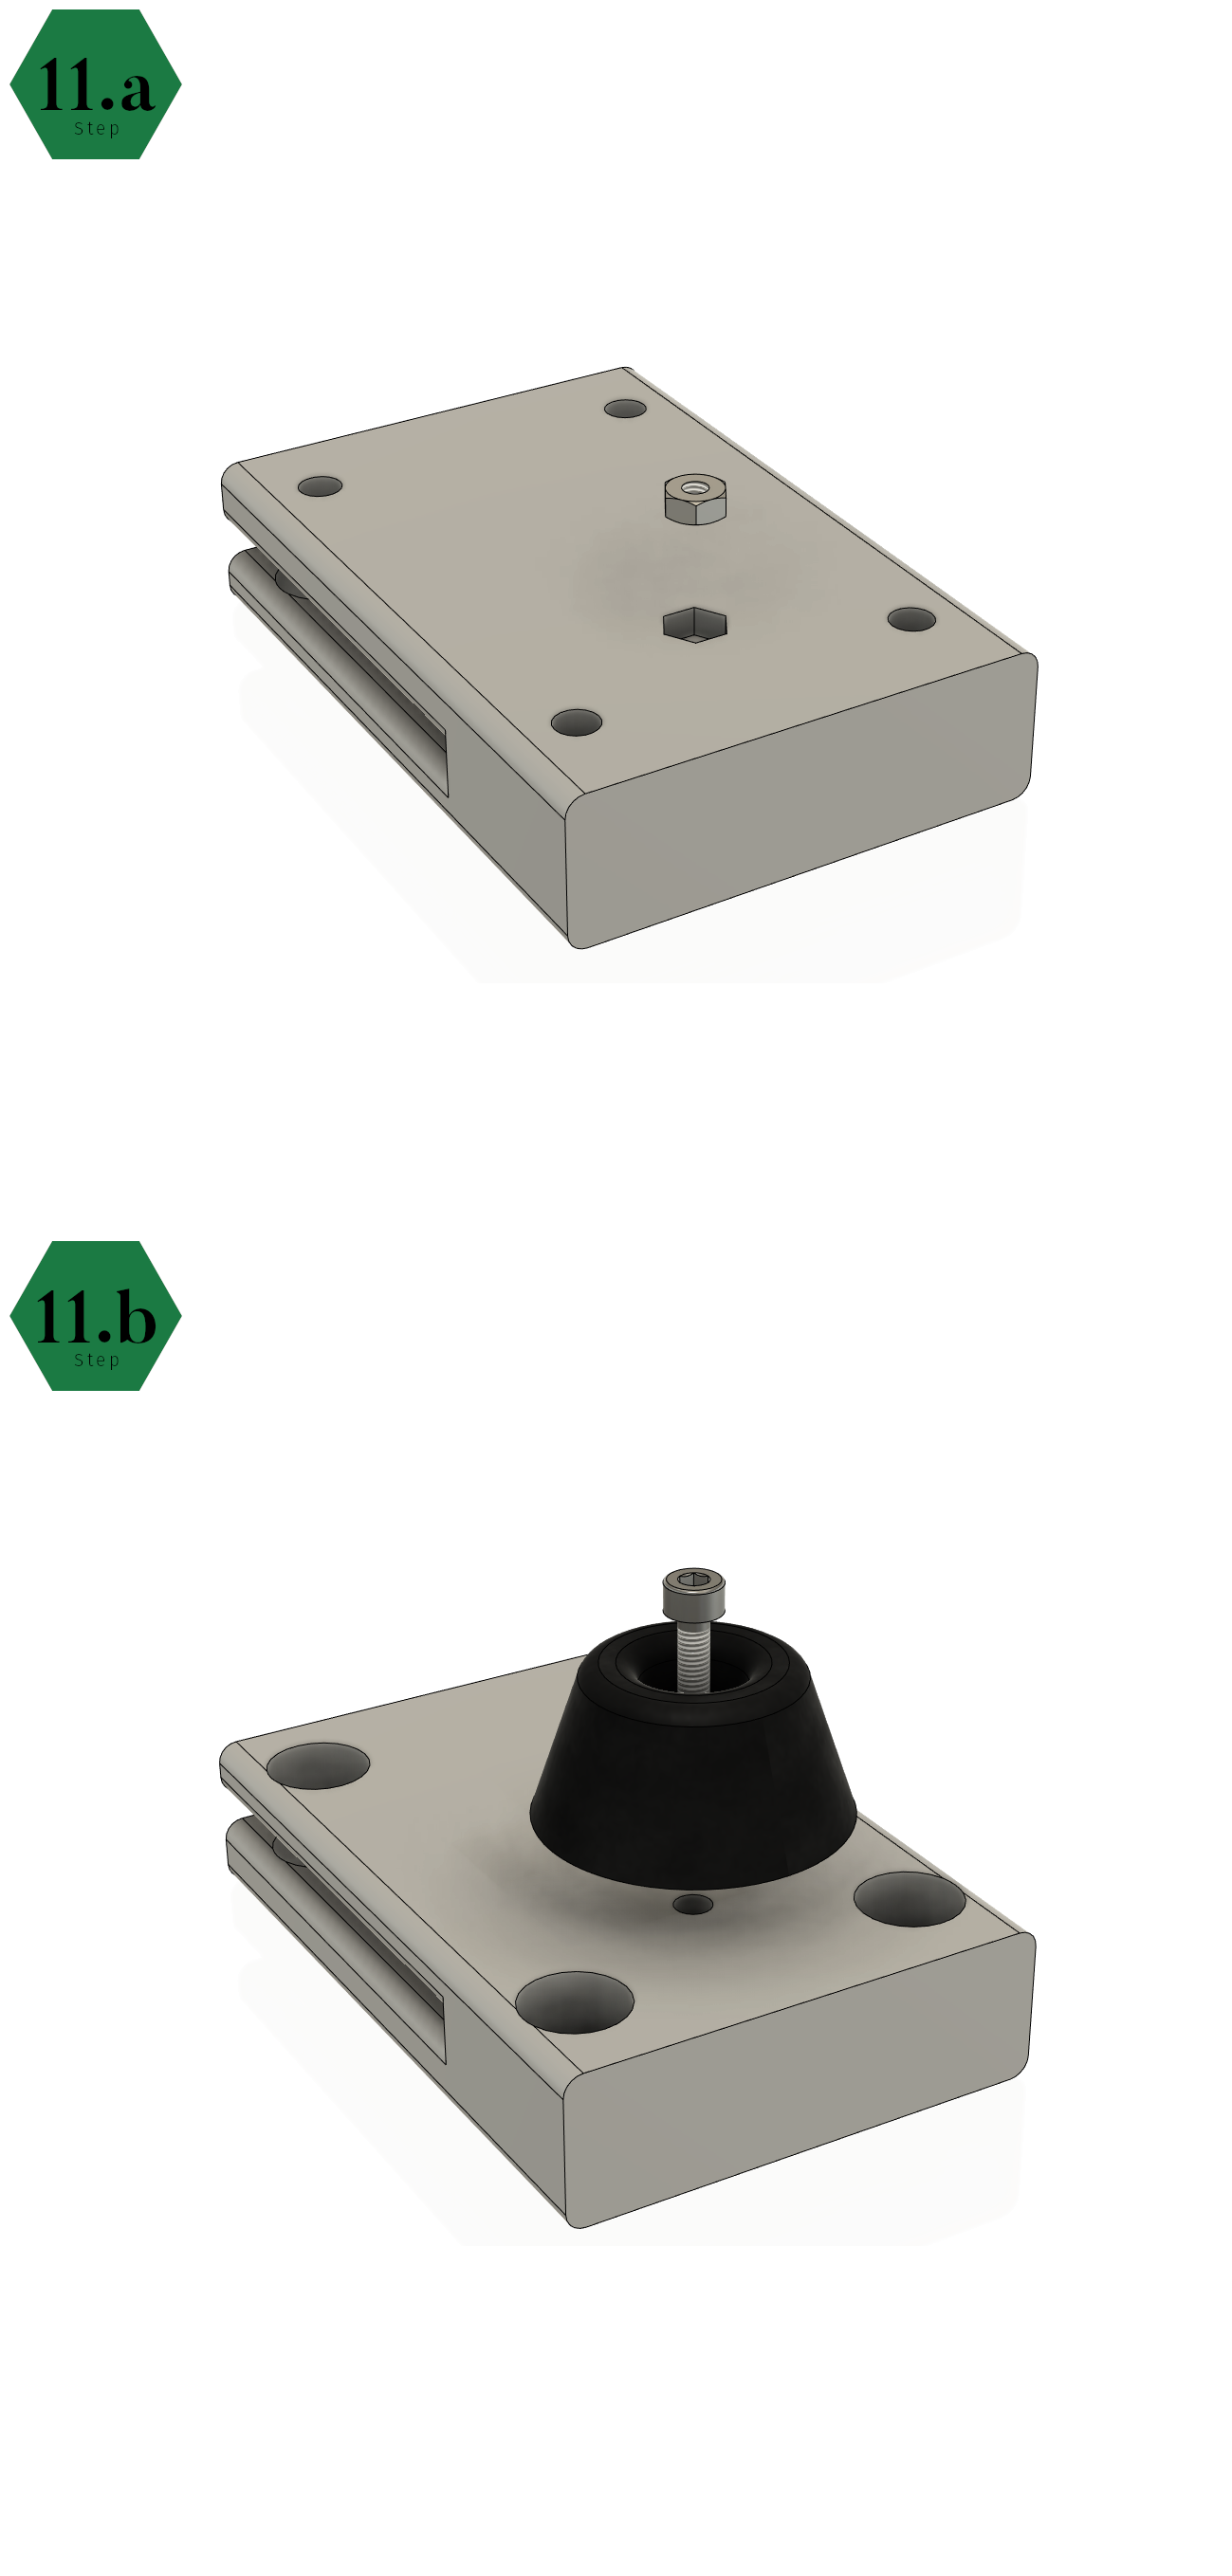
\includegraphics{images/Assembly8.png}%
{\captionof{figure}{Step 11 of the Open3DScanner assembly}}
\clearpage%

% STEP 12
\sideTabularx[Required parts for step 12]{%
	\rowcolors{2}{tableLineTwo}{tableLineOne}% specify rowcolors in tabularx style
	\begin{tabularx} {\marginparwidth} {>{\rowmac \hsize=1.5\hsize}X>{\rowmac \hsize=0.5\hsize}X<{\clearrow}}%
		\tabularxHeader%
		Part & Quantity\\%
		\SI{400}{\milli\meter} $\times$ \SI{550}{\milli\meter} $\times$ \SI{16}{\milli\meter} Wooden Board & 1\\%
		Backplate-Holder & 2\\%
		4.0$\times$16 Countersunk Wood Screwt & 24\\%
	\end{tabularx}%
}%

\marginInfo*[Instructions]{Screw the parts to the wooden board which is used as base plate. Use four screws for each assembled foot and Backplate-Holder. On the underside of the wooden board, mount one foot flush in each corner. The horizontal opening points into the inner area of the plate. The openings of two feet, which are mounted along the long edge of the base plate, face each other. The backplate holders are mounted from the top of the base plate. They are mounted flush in the corners of one of the long edges of the wooden board. The Backplate-Holder inserts have to be parallel to the long edge of the base plate.}%

\marginTips*[Tip]{You need to mount four assembled feets and two Backplate-Holder.}%

\marginCritical*[Warning]{Align the components as well as possible at the corners of the wooden board. Otherwise it can happen that the rear panel does not fit properly or that parts cannot be screwed down because the screws on the top and bottom side collide.}%

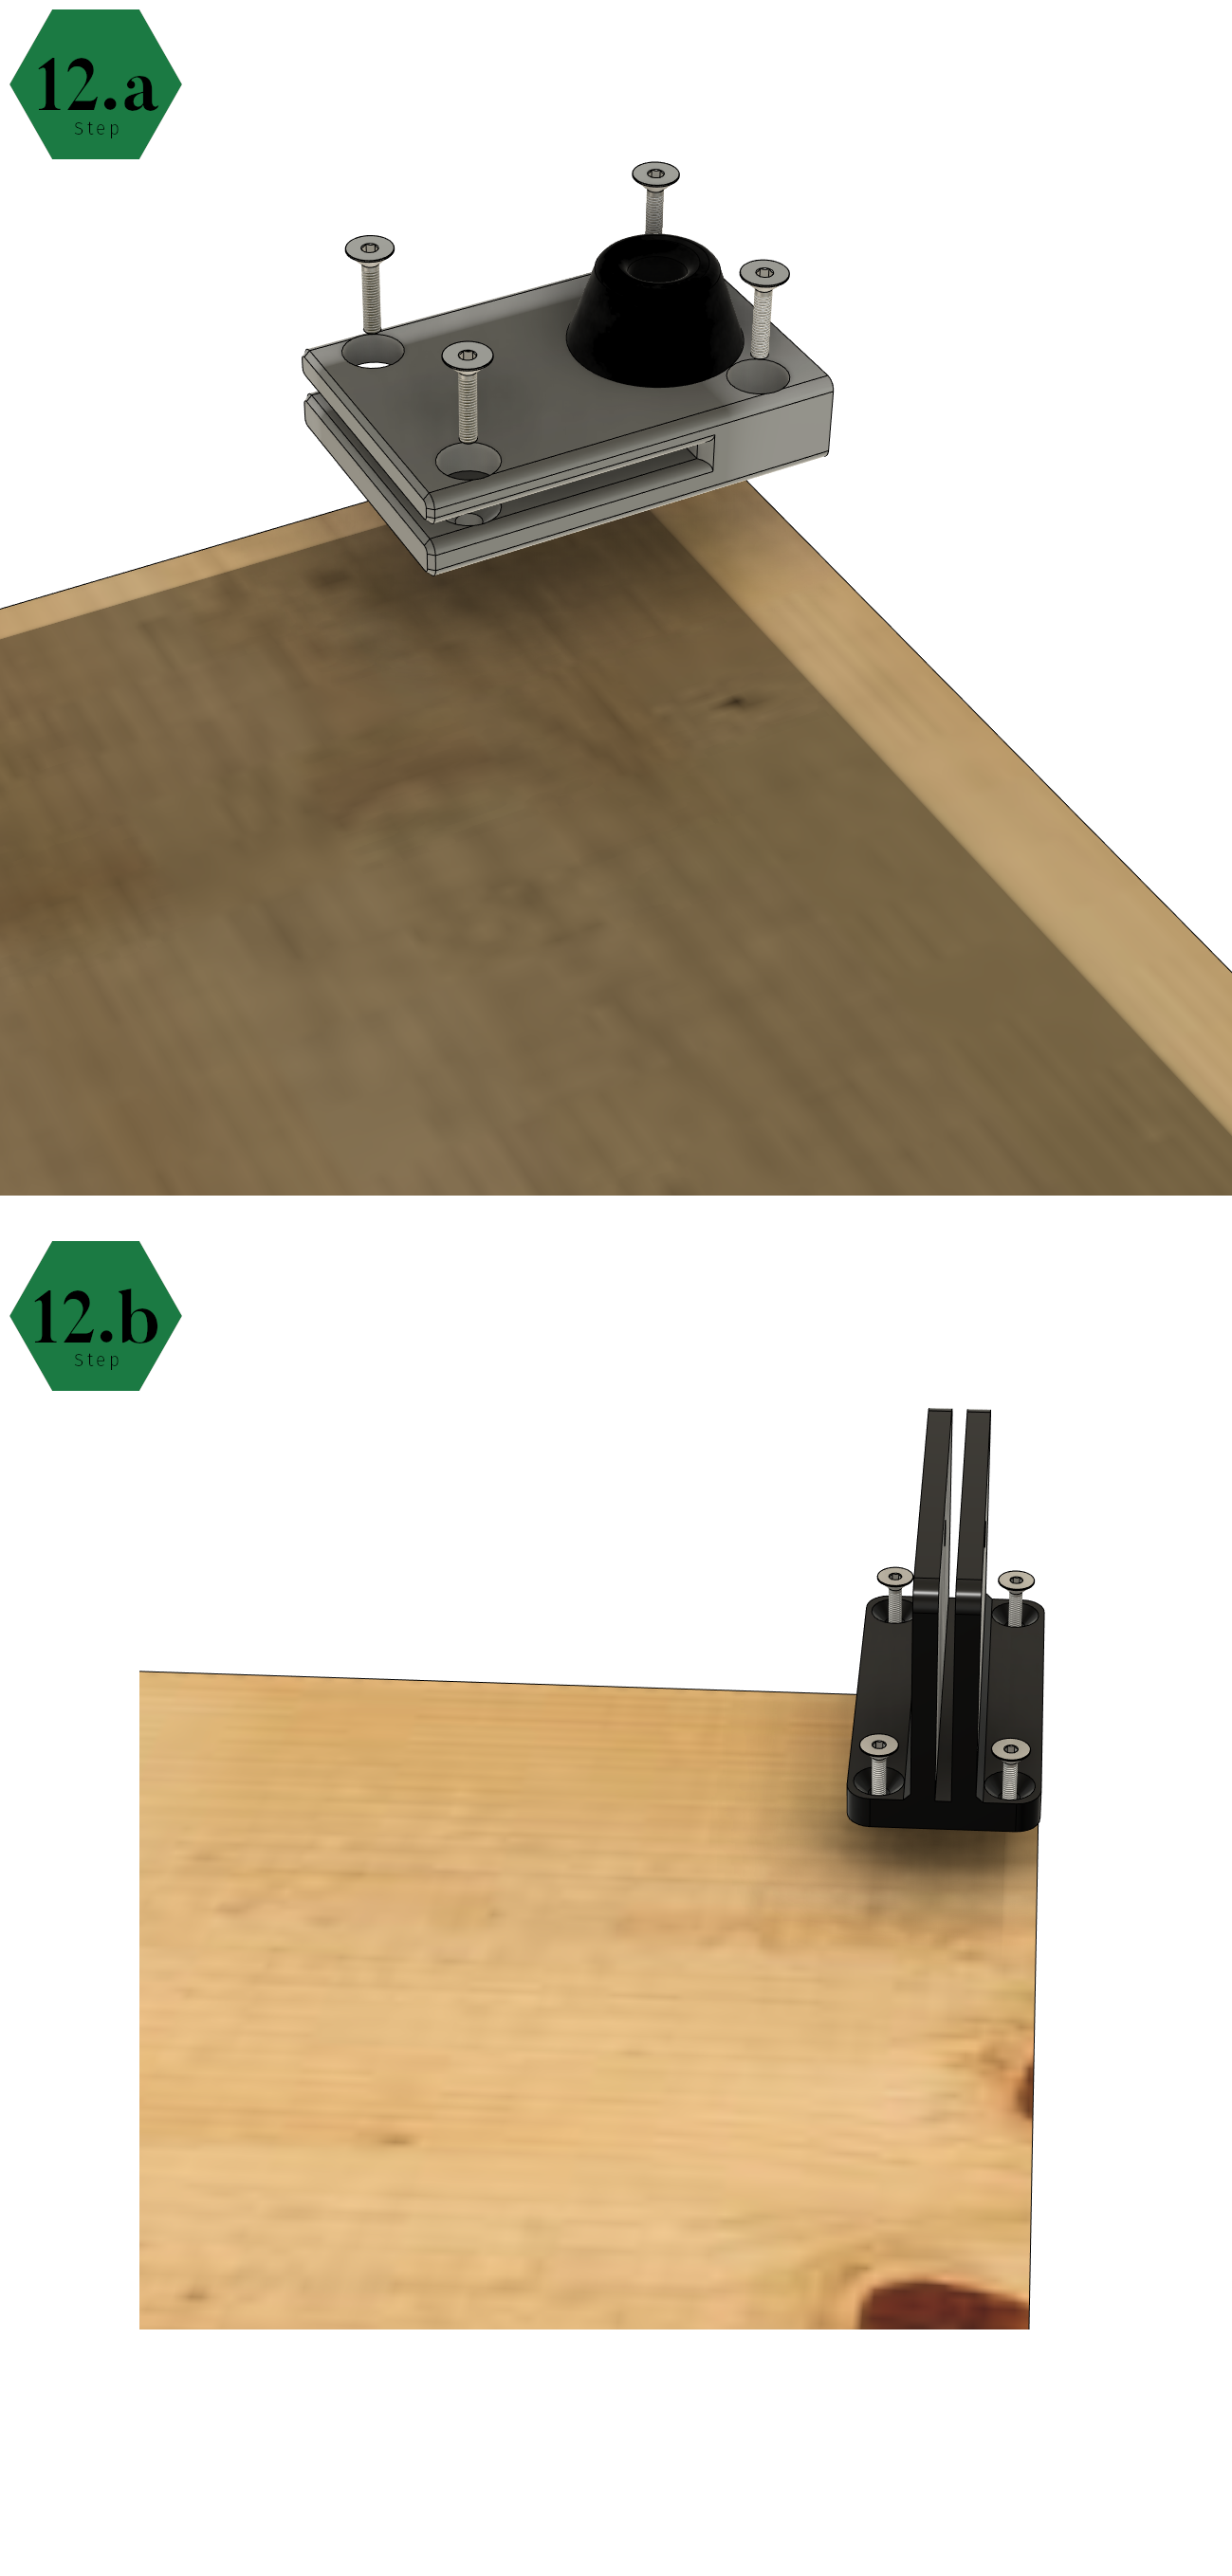
\includegraphics{images/Assembly9.png}%
{\captionof{figure}{Step 12 of the Open3DScanner assembly}}
\clearpage%

% STEP 13
\sideTabularx[Required parts for step 13]{%
	\rowcolors{2}{tableLineTwo}{tableLineOne}% specify rowcolors in tabularx style
	\begin{tabularx} {\marginparwidth} {>{\rowmac \hsize=1.5\hsize}X>{\rowmac \hsize=0.5\hsize}X<{\clearrow}}%
		\tabularxHeader%
		Part & Quantity\\%
		Housing-Main & 1\\%
		\SI{5.5}{\milli\meter}$\times$\SI{2.1}{\milli\meter} Female DC Power Jack Panel Mount (L722AS) & 1\\%
		\SI{5/8}{''} Rubber Seal Ring & 1\\%
	\end{tabularx}%
}%

\marginInfo*[Instructions]{Press the rubber seal into the opening provided in the back of the housing. Mount the power jack in the opening on the left side of the case.}%

\marginTips*[Tip]{If your power jack does not have the accessories for mounting, you will need a M8 nut and a \SI{1}{\milli\meter} washer with \SI{8}{\milli\meter} diameter in addition. Pliers simplify the tightening of the nut. In order to simplify the wiring, it makes sense to attach the power cable to the jack first.}%

\marginCritical*[Warning]{Make sure that the power jack is aligned as shown in the illustration, otherwise the PCB may not fit into the case anymore.}%

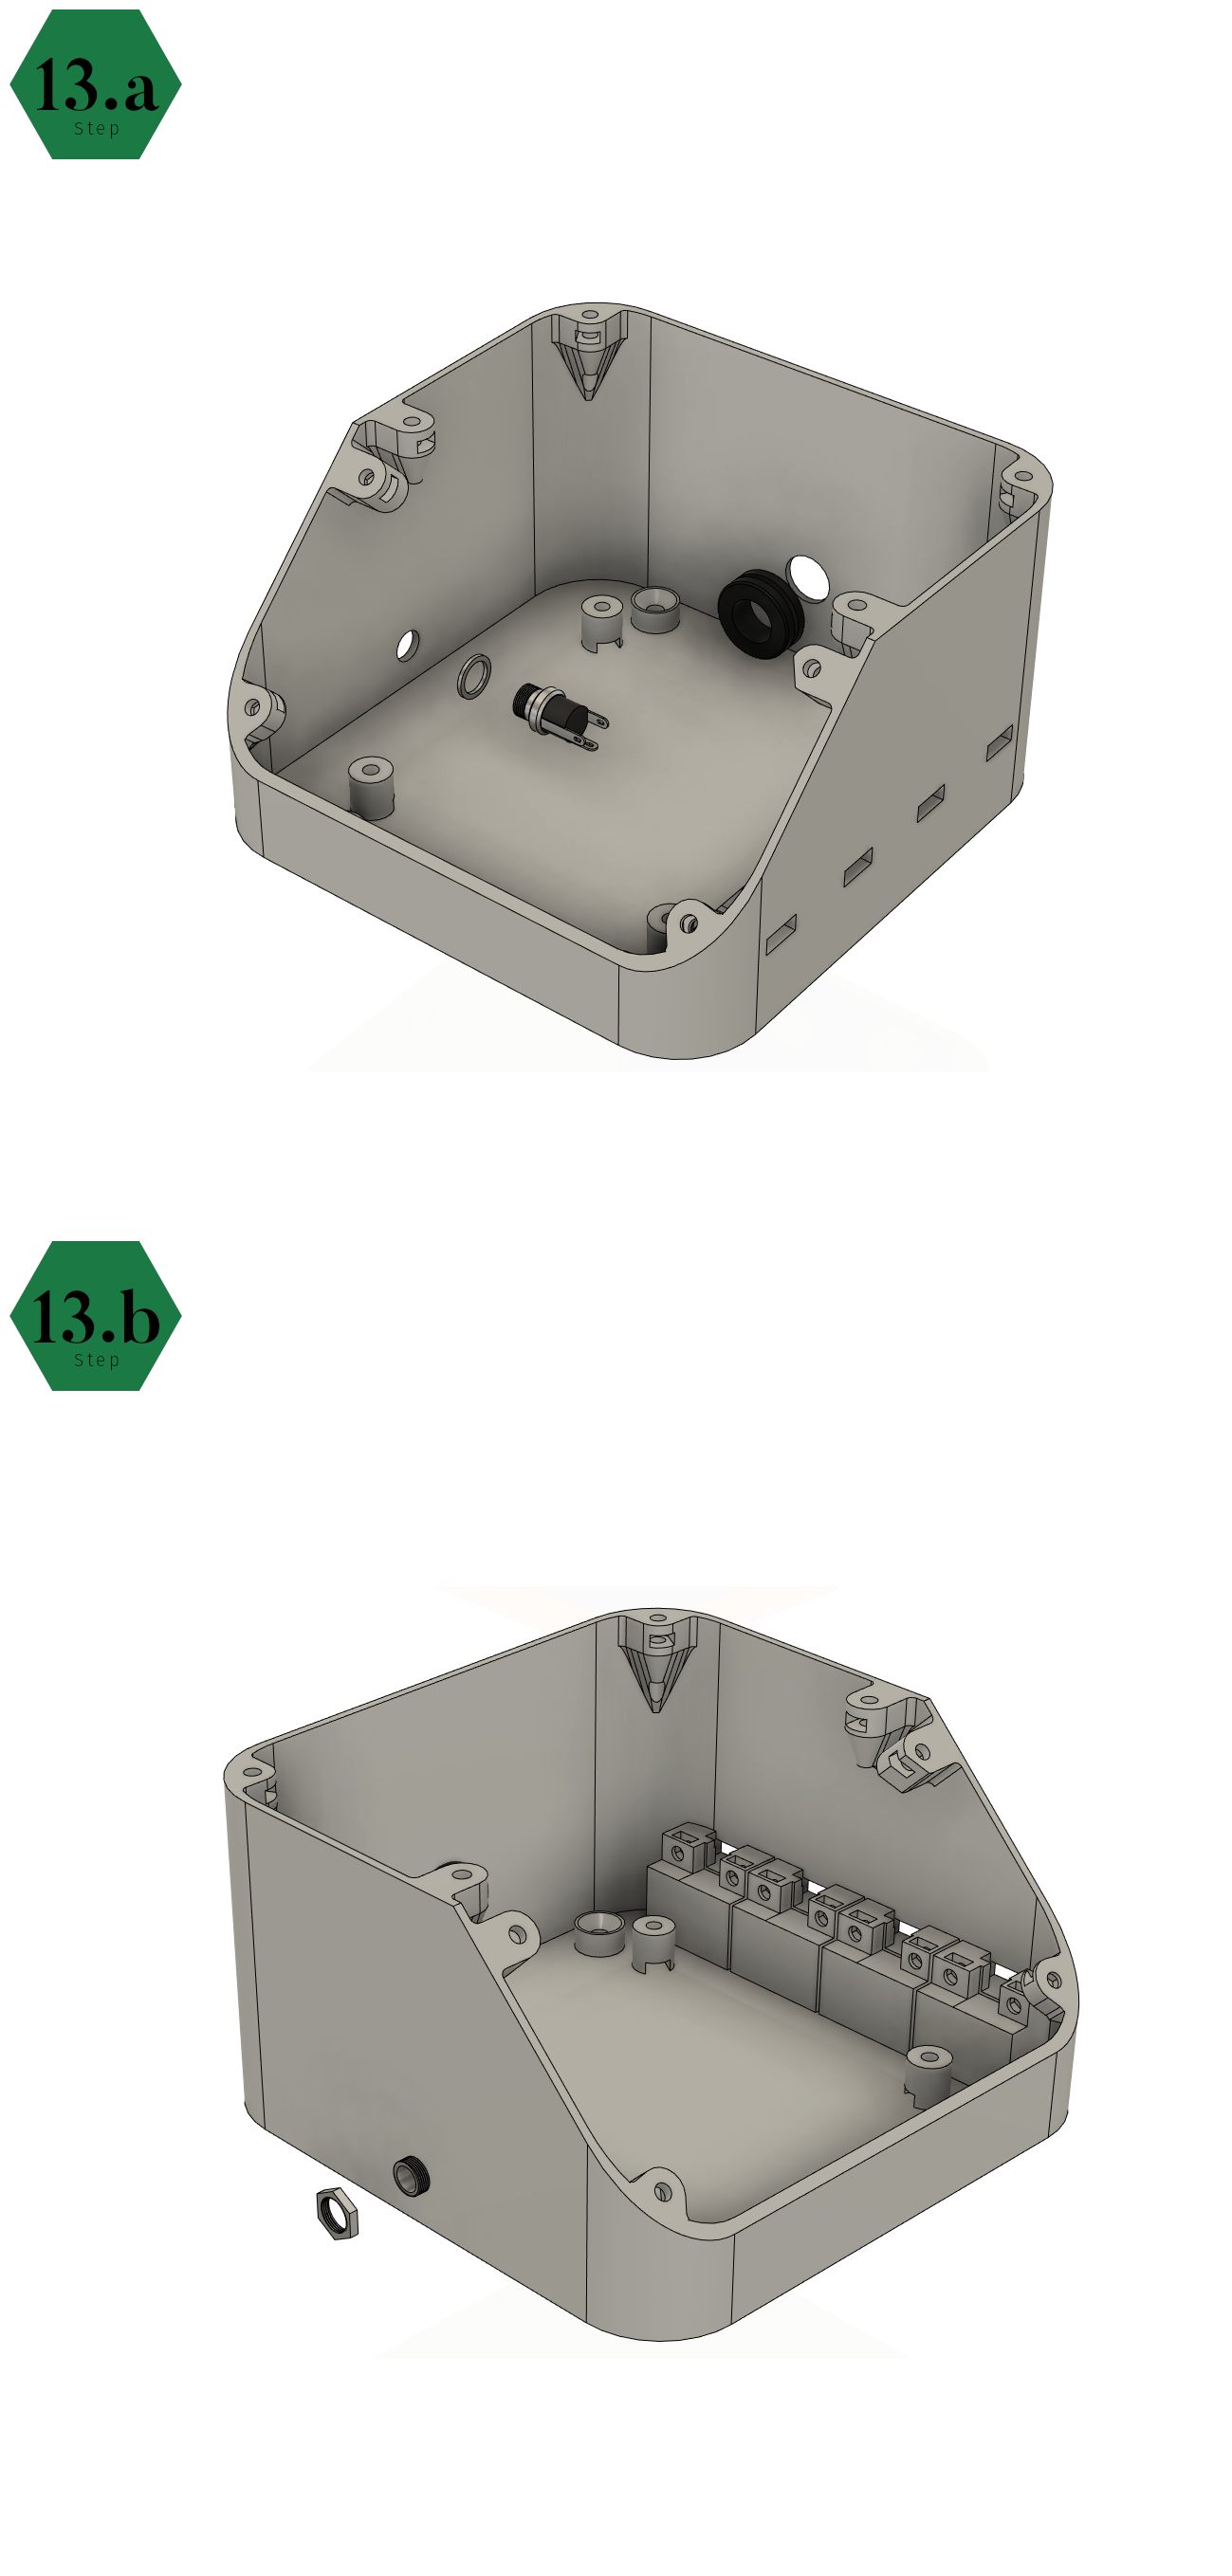
\includegraphics{images/Assembly10.png}%
{\captionof{figure}{Step 13 of the Open3DScanner assembly}}
\clearpage%

% STEP 14
\sideTabularx[Required parts for step 14]{%
	\rowcolors{2}{tableLineTwo}{tableLineOne}% specify rowcolors in tabularx style
	\begin{tabularx} {\marginparwidth} {>{\rowmac \hsize=1.5\hsize}X>{\rowmac \hsize=0.5\hsize}X<{\clearrow}}%
		\tabularxHeader%
		Part & Quantity\\%
		Molex crimp housing --- Micro-Fit - 1x2-pin, male (430200201) & 4\\%
		M3 Nut & 8\\%
	\end{tabularx}%
}%

\marginInfo*[Instructions]{Mount the Micro-Fit connectors. Make sure that the mounting hook points to the rear of the housing. The connectors are first pressed against the housing wall and pushed into the recess. Then they are pushed out a little bit so that they are flush with the outside of the housing. Slide the nuts into the openings.  Two nuts are required for each connector.}%

\marginTips*[Tip]{Before mounting the Micro-Fit connectors, connect the cables to them.}%

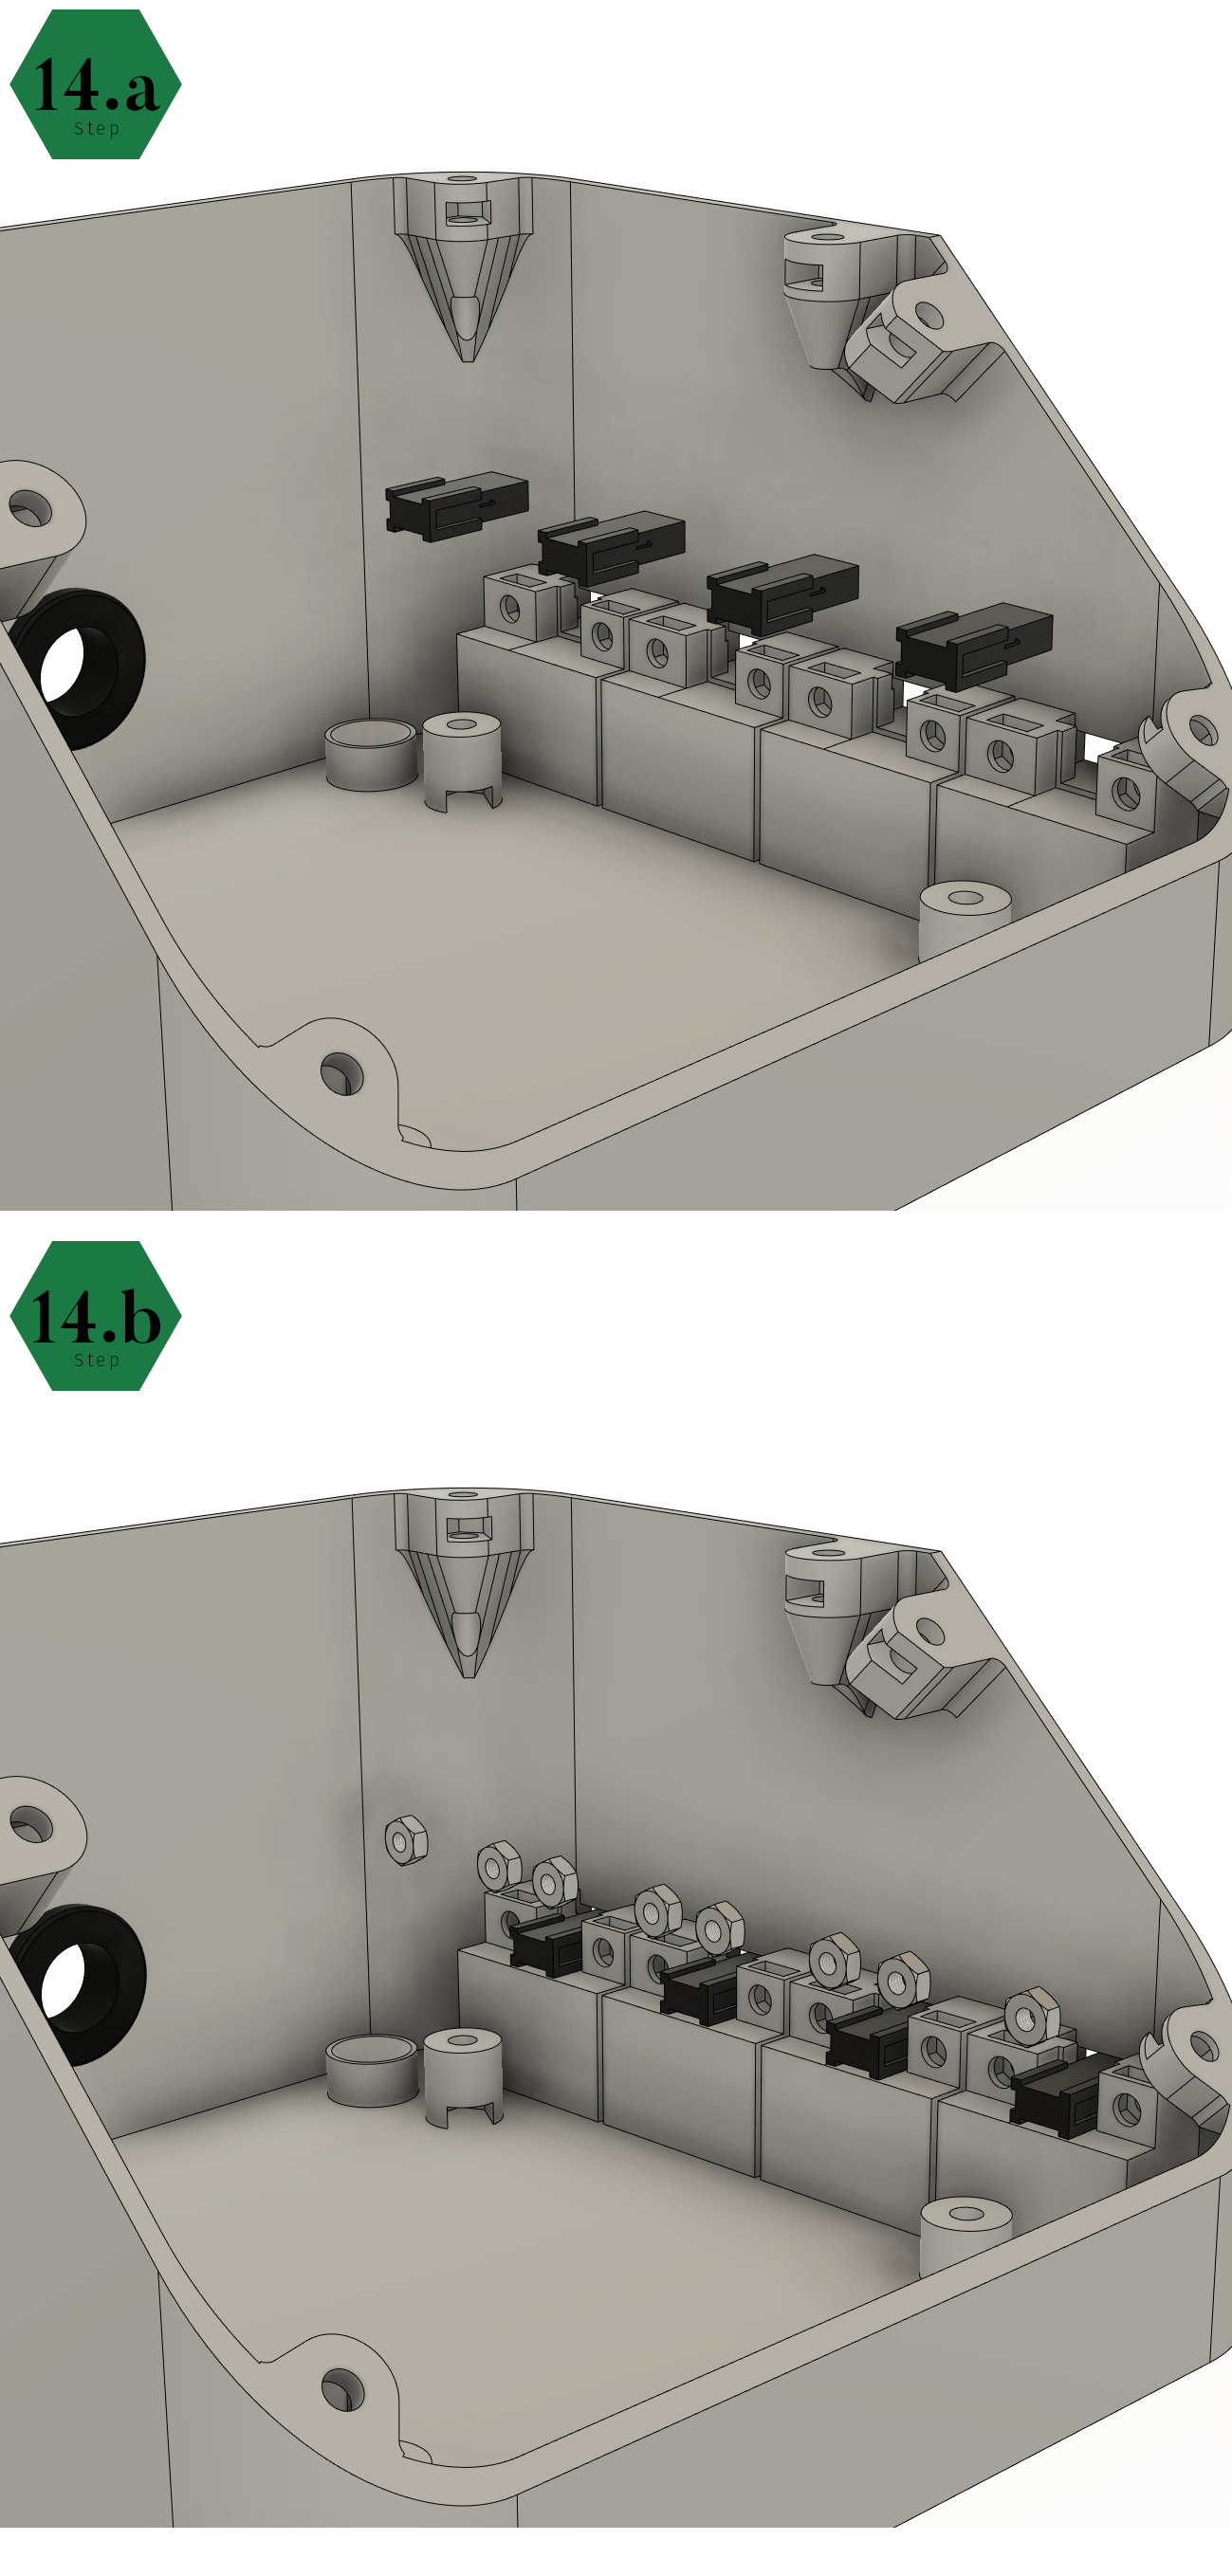
\includegraphics{images/Assembly11.png}%
{\captionof{figure}{Step 14 of the Open3DScanner assembly}}
\clearpage%

% STEP 15 & 16
\sideTabularx[Required parts for step 15]{%
	\rowcolors{2}{tableLineTwo}{tableLineOne}% specify rowcolors in tabularx style
	\begin{tabularx} {\marginparwidth} {>{\rowmac \hsize=1.5\hsize}X>{\rowmac \hsize=0.5\hsize}X<{\clearrow}}%
		\tabularxHeader%
		Part & Quantity\\%
		Micro-Fit-Holder-P1 & 4\\%
		Micro-Fit-Holder-P2 & 4\\%
		M3$\times$10 & 8\\%
	\end{tabularx}%
}%

\marginInfo*[Instructions]{Use one Micro-Fit-Holder-P1, one Micro-Fit-Holder-P1, and two screws to secure each Micro-Fit connectors.}%

\sideTabularx[Required parts for step 16]{%
	\vspace{4.5cm}%
	\rowcolors{2}{tableLineTwo}{tableLineOne}% specify rowcolors in tabularx style
	\begin{tabularx} {\marginparwidth} {>{\rowmac \hsize=1.5\hsize}X>{\rowmac \hsize=0.5\hsize}X<{\clearrow}}%
		\tabularxHeader%
		Part & Quantity\\%
		M3 Nut & 8\\%
	\end{tabularx}%
}%

\marginInfo*[Instructions]{Slide a nut into each opening along the top edge of the housing.}%

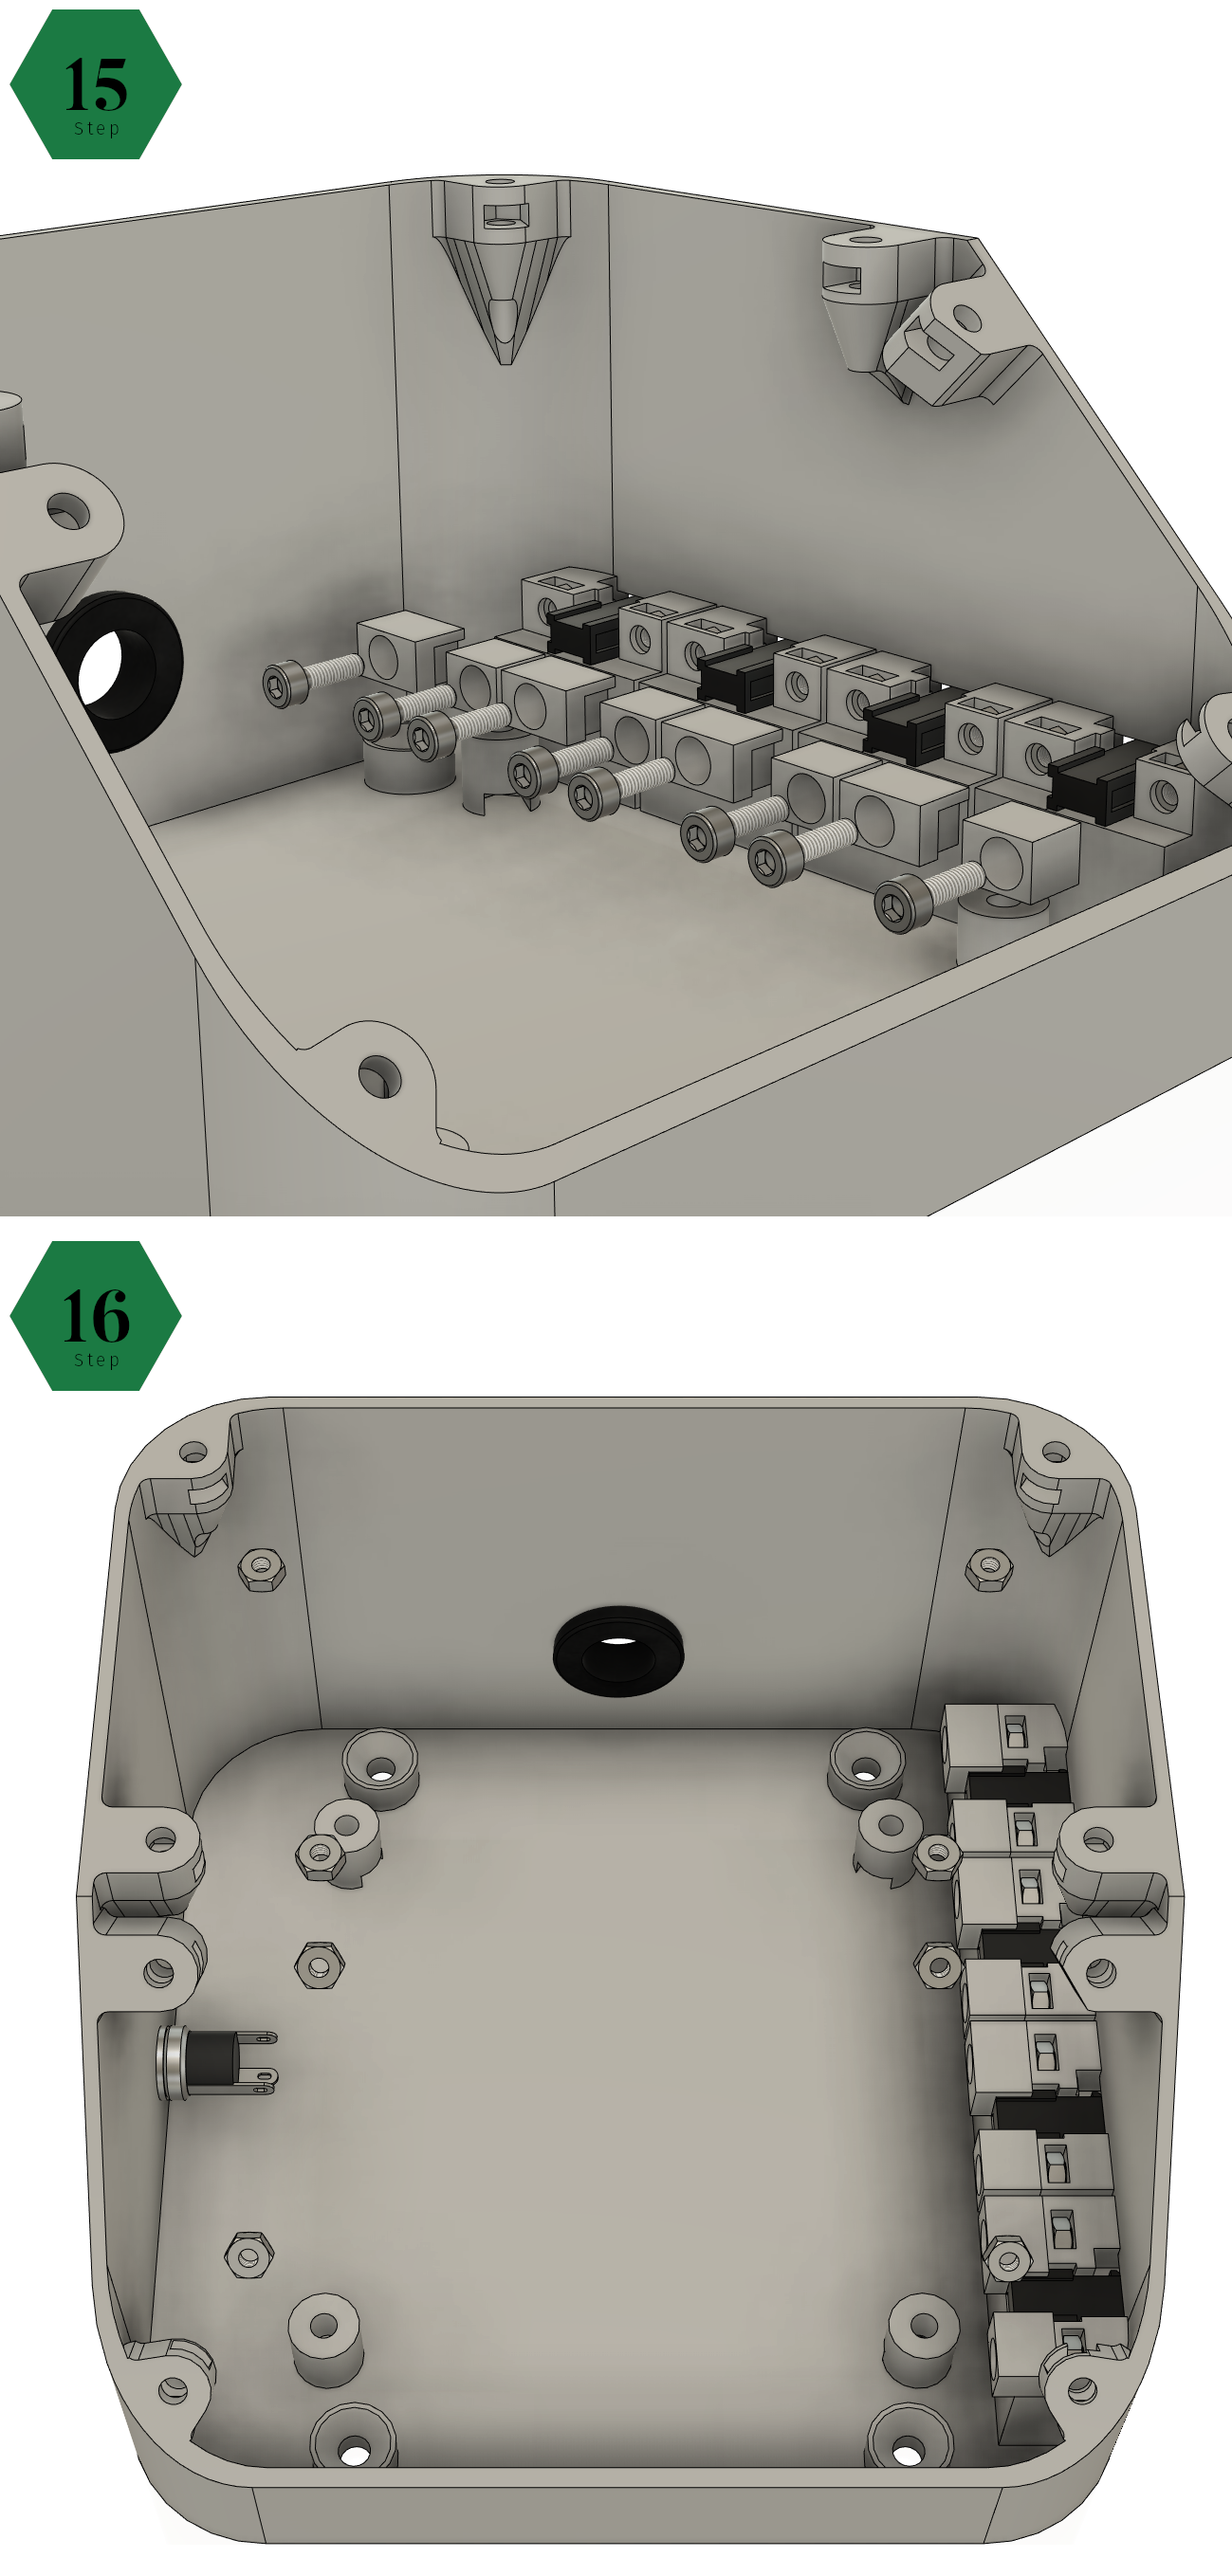
\includegraphics{images/Assembly12.png}%
{\captionof{figure}{Step 15 \& 16 of the Open3DScanner assembly}}
\clearpage%

% STEP 17
\sideTabularx[Required parts for step 17]{%
	\rowcolors{2}{tableLineTwo}{tableLineOne}% specify rowcolors in tabularx style
	\begin{tabularx} {\marginparwidth} {>{\rowmac \hsize=1.5\hsize}X>{\rowmac \hsize=0.5\hsize}X<{\clearrow}}%
		\tabularxHeader%
		Part & Quantity\\%
		PCB & 1\\%
		M3 Nut & 4\\%
		M3$\times$12 & 4\\%
	\end{tabularx}%
}%

\marginInfo*[Instructions]{Slide one nut each into the PCB stand at the bottom of the housing. Then screw the PCB into the housing.}%

\marginTips*[Tip]{The cable from the power jack can be routed below the PCB. This is much easier if it is done before the PCB is screwed down.}%

\marginCheck*[Check]{Make sure that you align the PCB as shown in the figure, otherwise the wiring may become difficult and the specified cable lengths will no longer fit.}%

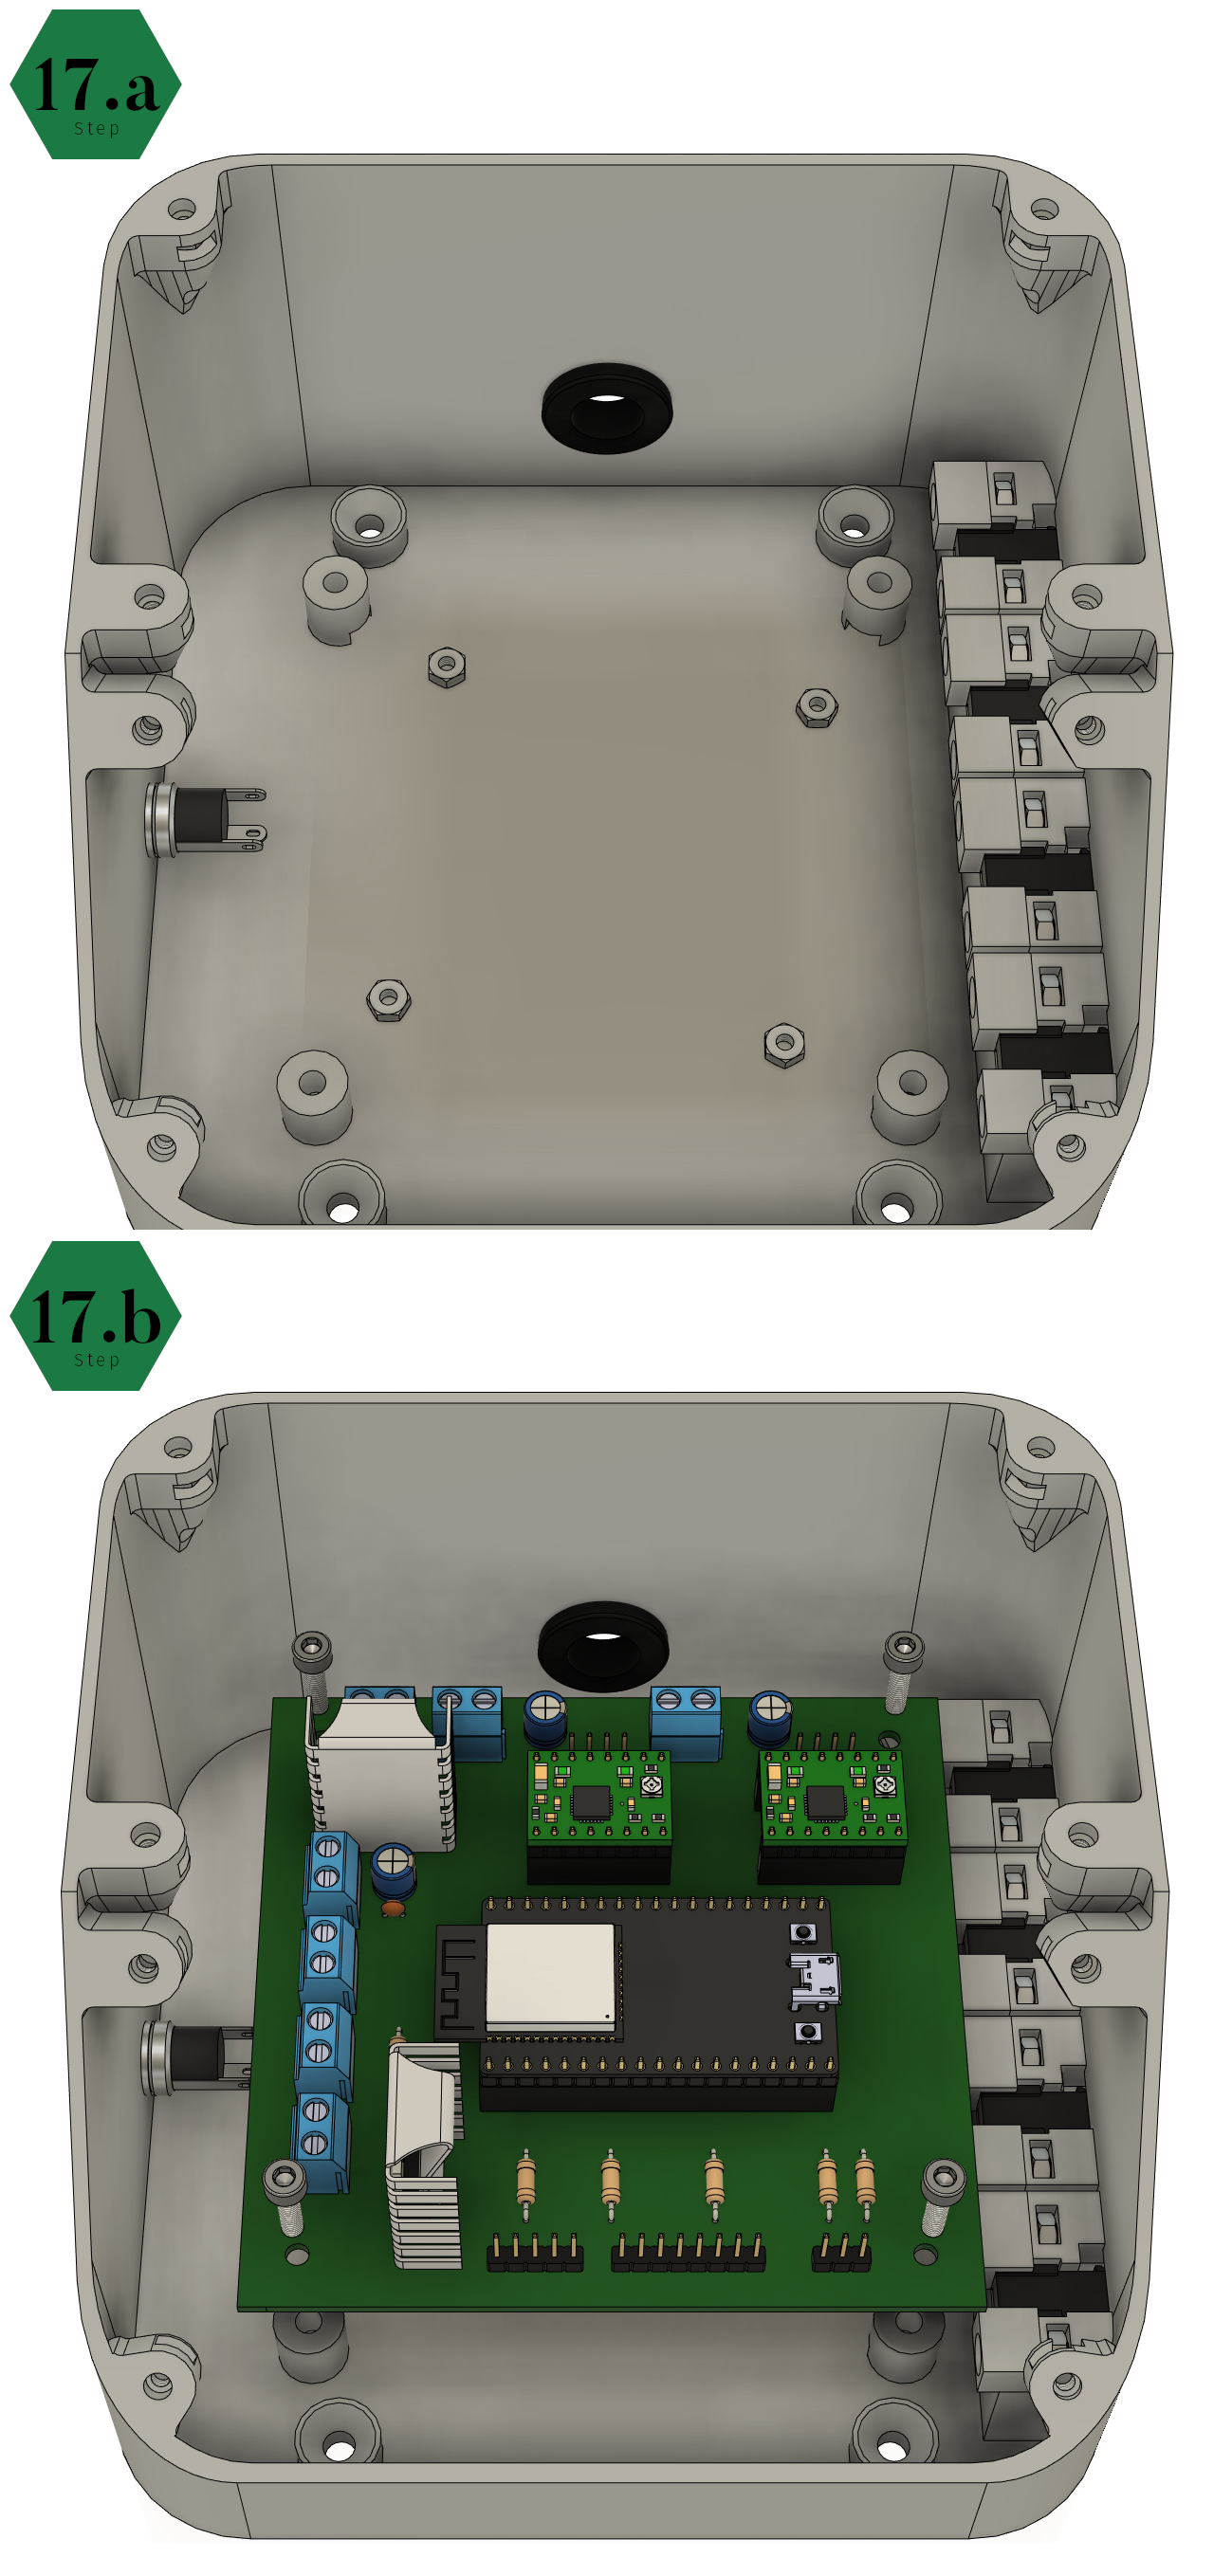
\includegraphics{images/Assembly13.png}%
{\captionof{figure}{Step 17 of the Open3DScanner assembly}}
\clearpage%

% STEP 18 & 19
\sideTabularx[Required parts for step 18]{%
	\rowcolors{2}{tableLineTwo}{tableLineOne}% specify rowcolors in tabularx style
	\begin{tabularx} {\marginparwidth} {>{\rowmac \hsize=1.5\hsize}X>{\rowmac \hsize=0.5\hsize}X<{\clearrow}}%
		\tabularxHeader%
		Part & Quantity\\%
		4.0$\times$16 Countersunk Wood Screwt & 4\\%
	\end{tabularx}%
}%

\marginInfo*[Instructions]{Screw the housing onto the wooden base plate.}%

\marginTips*[Tip]{For the exact alignment on the base plate, there is a detailed illustration at the end of the assembly instructions.}%

\sideTabularx[Required parts for step 19]{%
	\vspace{1.80cm}%
	\rowcolors{2}{tableLineTwo}{tableLineOne}% specify rowcolors in tabularx style
	\begin{tabularx} {\marginparwidth} {>{\rowmac \hsize=1.5\hsize}X>{\rowmac \hsize=0.5\hsize}X<{\clearrow}}%
		\tabularxHeader%
		Part & Quantity\\%
		STEC12E08 Rotary Encoder & 1\\%
		\SI{5}{\milli\meter} 3-Pin Bi-Color LED & 1\\%
		Nokia 5110 Display & 1\\%
		LCD-Holder & 4\\%
		LED-Holder & 1\\%
		Encoder-Holder & 1\\%
		Housing-Front & 1\\%
		M3$\times$12 & 2\\%
		M3$\times$6 & 2\\%
		M3 Nut & 8\\%
	\end{tabularx}%
}%

\marginInfo*[Instructions]{Glue the nuts for the LED and the encoder with superglue into the front panel of the housing. Press the remaining nuts into the LCD-holder. Insert the LED, encoder, and LCD into the openings provided in the front panel. Screw the LED and encoder to the front panel. Use LED-Holder and Encoder-Holder for this.}%

\marginTips*[Tip]{Depending on the manufacturer of the LCD, it may be necessary to cut a piece out of the back of the front panel, otherwise the solder points will prevent the display from sitting flush in the panel.}%

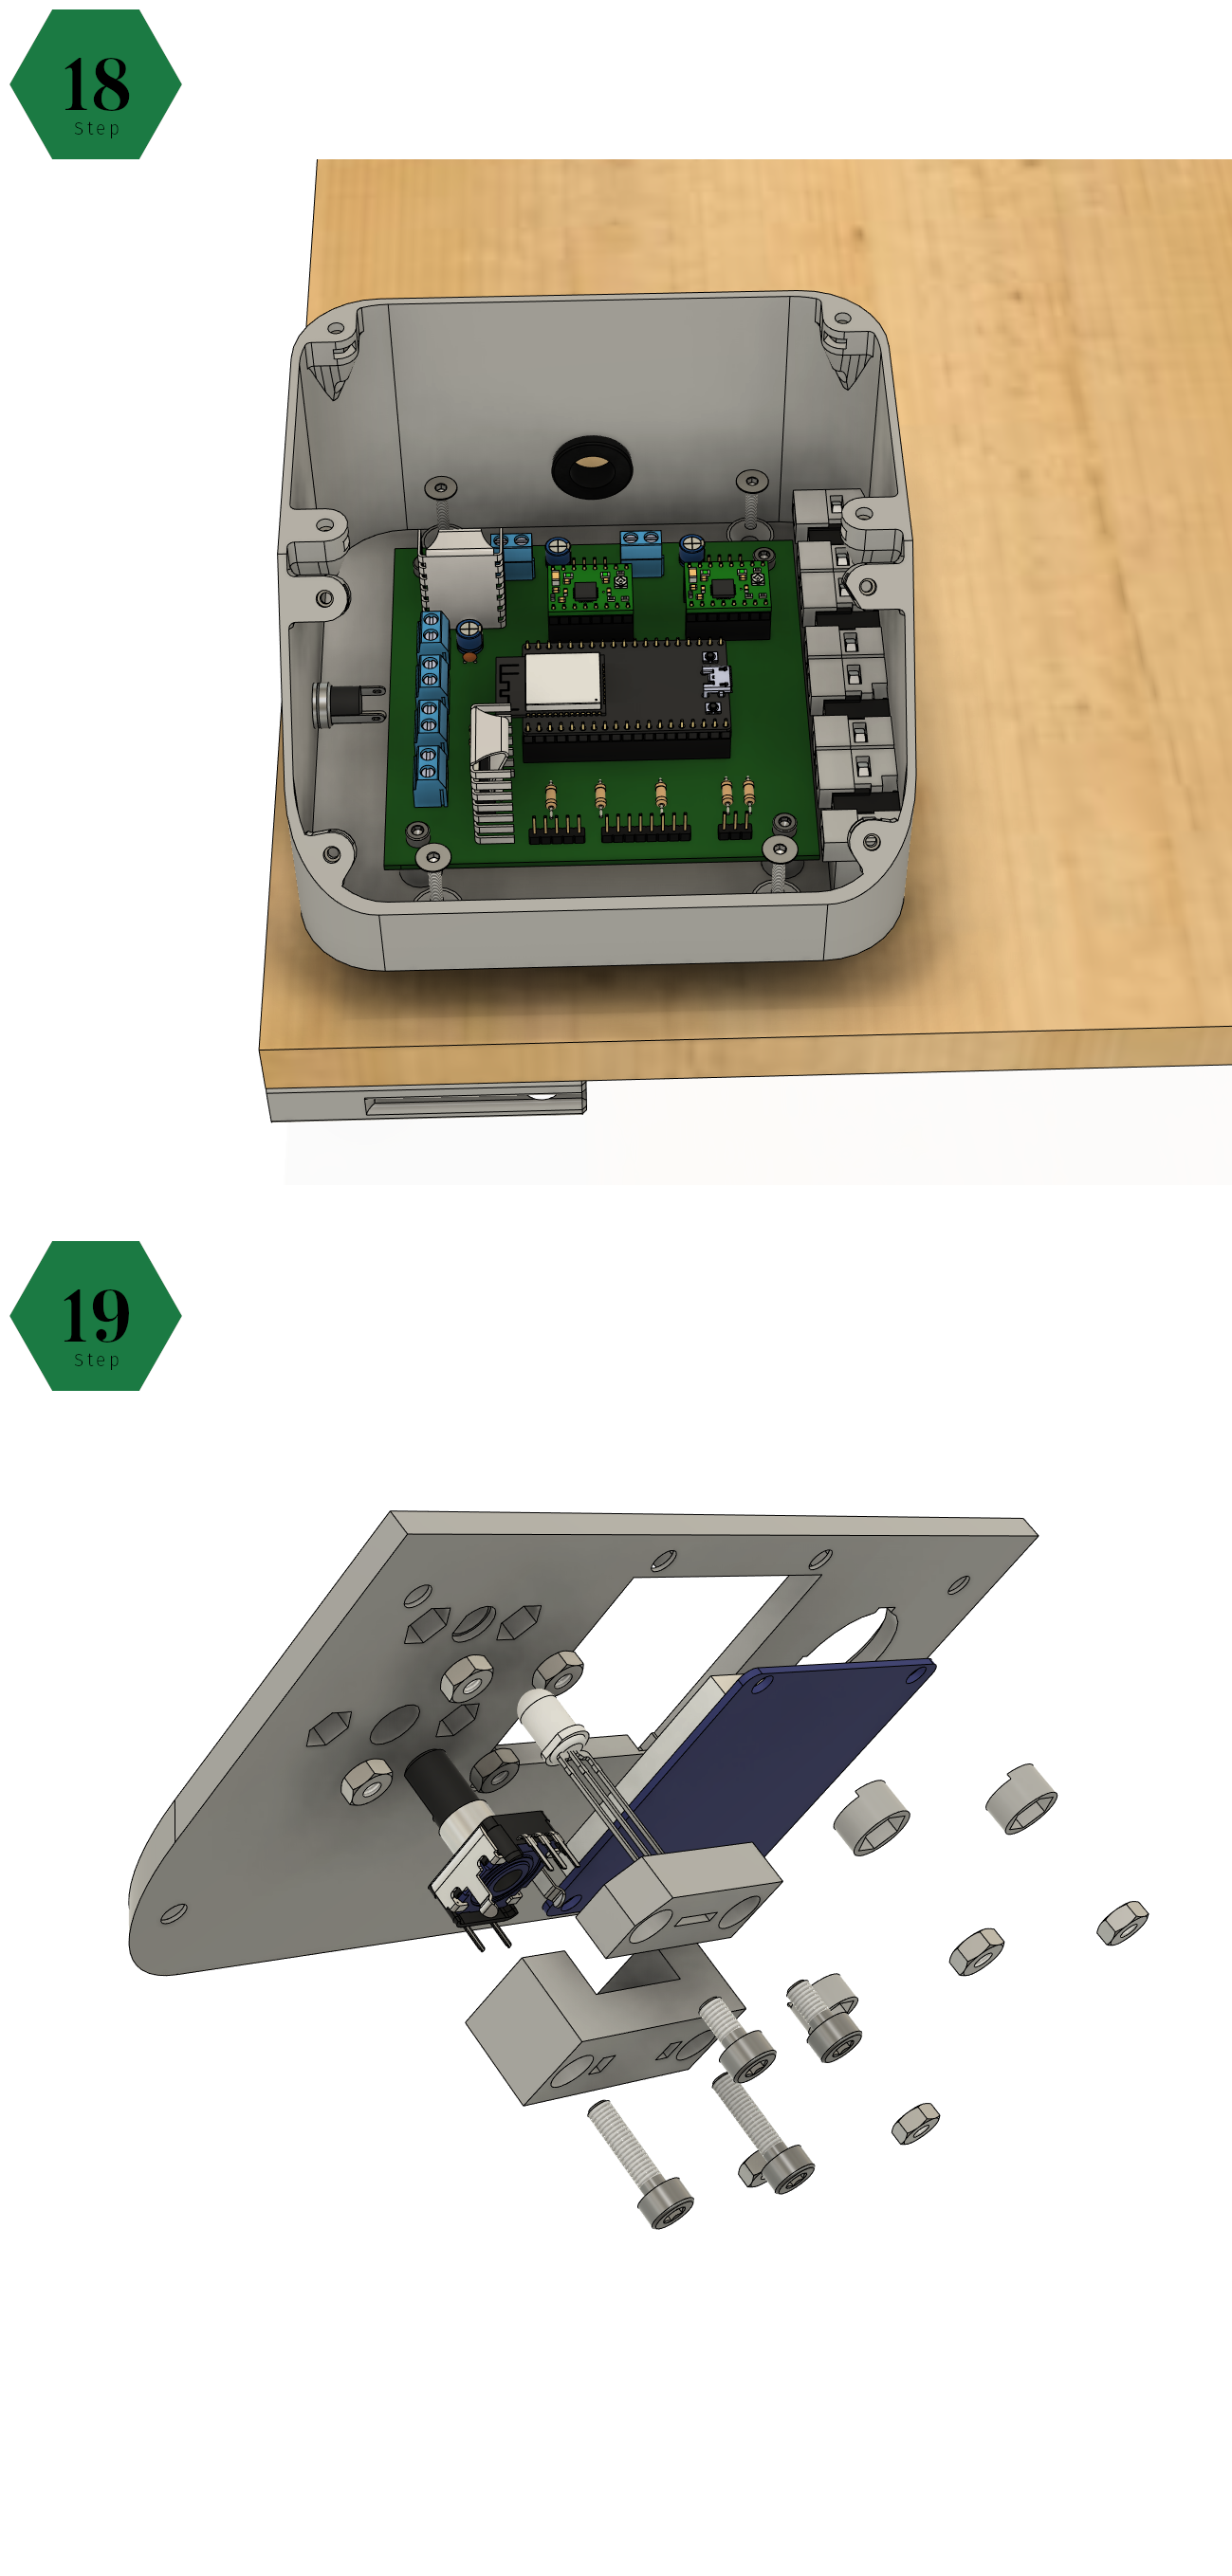
\includegraphics{images/Assembly14.png}%
{\captionof{figure}{Step 18 \& 19 of the Open3DScanner assembly}}
\clearpage%

% STEP 20 & 21
\sideTabularx[Required parts for step 20]{%
	\rowcolors{2}{tableLineTwo}{tableLineOne}% specify rowcolors in tabularx style
	\begin{tabularx} {\marginparwidth} {>{\rowmac \hsize=1.5\hsize}X>{\rowmac \hsize=0.5\hsize}X<{\clearrow}}%
		\tabularxHeader%
		Part & Quantity\\%
		Housing-Knob & 1\\%
		Round \SI{20}{\milli\meter} SPST Rocker Switch (R13 112) & 1\\%
		M3$\times$10  & 4\\%
	\end{tabularx}%
}%

\marginInfo*[Instructions]{Press the rocker switch into the recess of the front panel. Screw the display tight and pay attention to the orientation of the LCD-Holder. Press the Housing-Knob onto the shaft of the encoder.}%

\marginTips*[Tip]{Do not press the Housing-Knob too firmly on the shaft, otherwise the glued nuts will come loose.}%


\sideTabularx[Required parts for step 21]{%
	\vspace{0.80cm}%
	\rowcolors{2}{tableLineTwo}{tableLineOne}% specify rowcolors in tabularx style
	\begin{tabularx} {\marginparwidth} {>{\rowmac \hsize=1.5\hsize}X>{\rowmac \hsize=0.5\hsize}X<{\clearrow}}%
		\tabularxHeader%
		Part & Quantity\\%
		Housing-Top  & 1\\%
		M3$\times$10  & 8\\%
	\end{tabularx}%
}%

\marginInfo*[Instructions]{Screw the Housing-Top and the assembled Housing-Front to the housing.}%

\marginTips*[Tip]{Before you screw the front panel to the housing, all cables should be connected inside the housing and the stepper motors should also be connected to the PCB. Also ensure that you flashed the firmware to the ESP32. I recommend a basic functionality test before closing the housing.}%

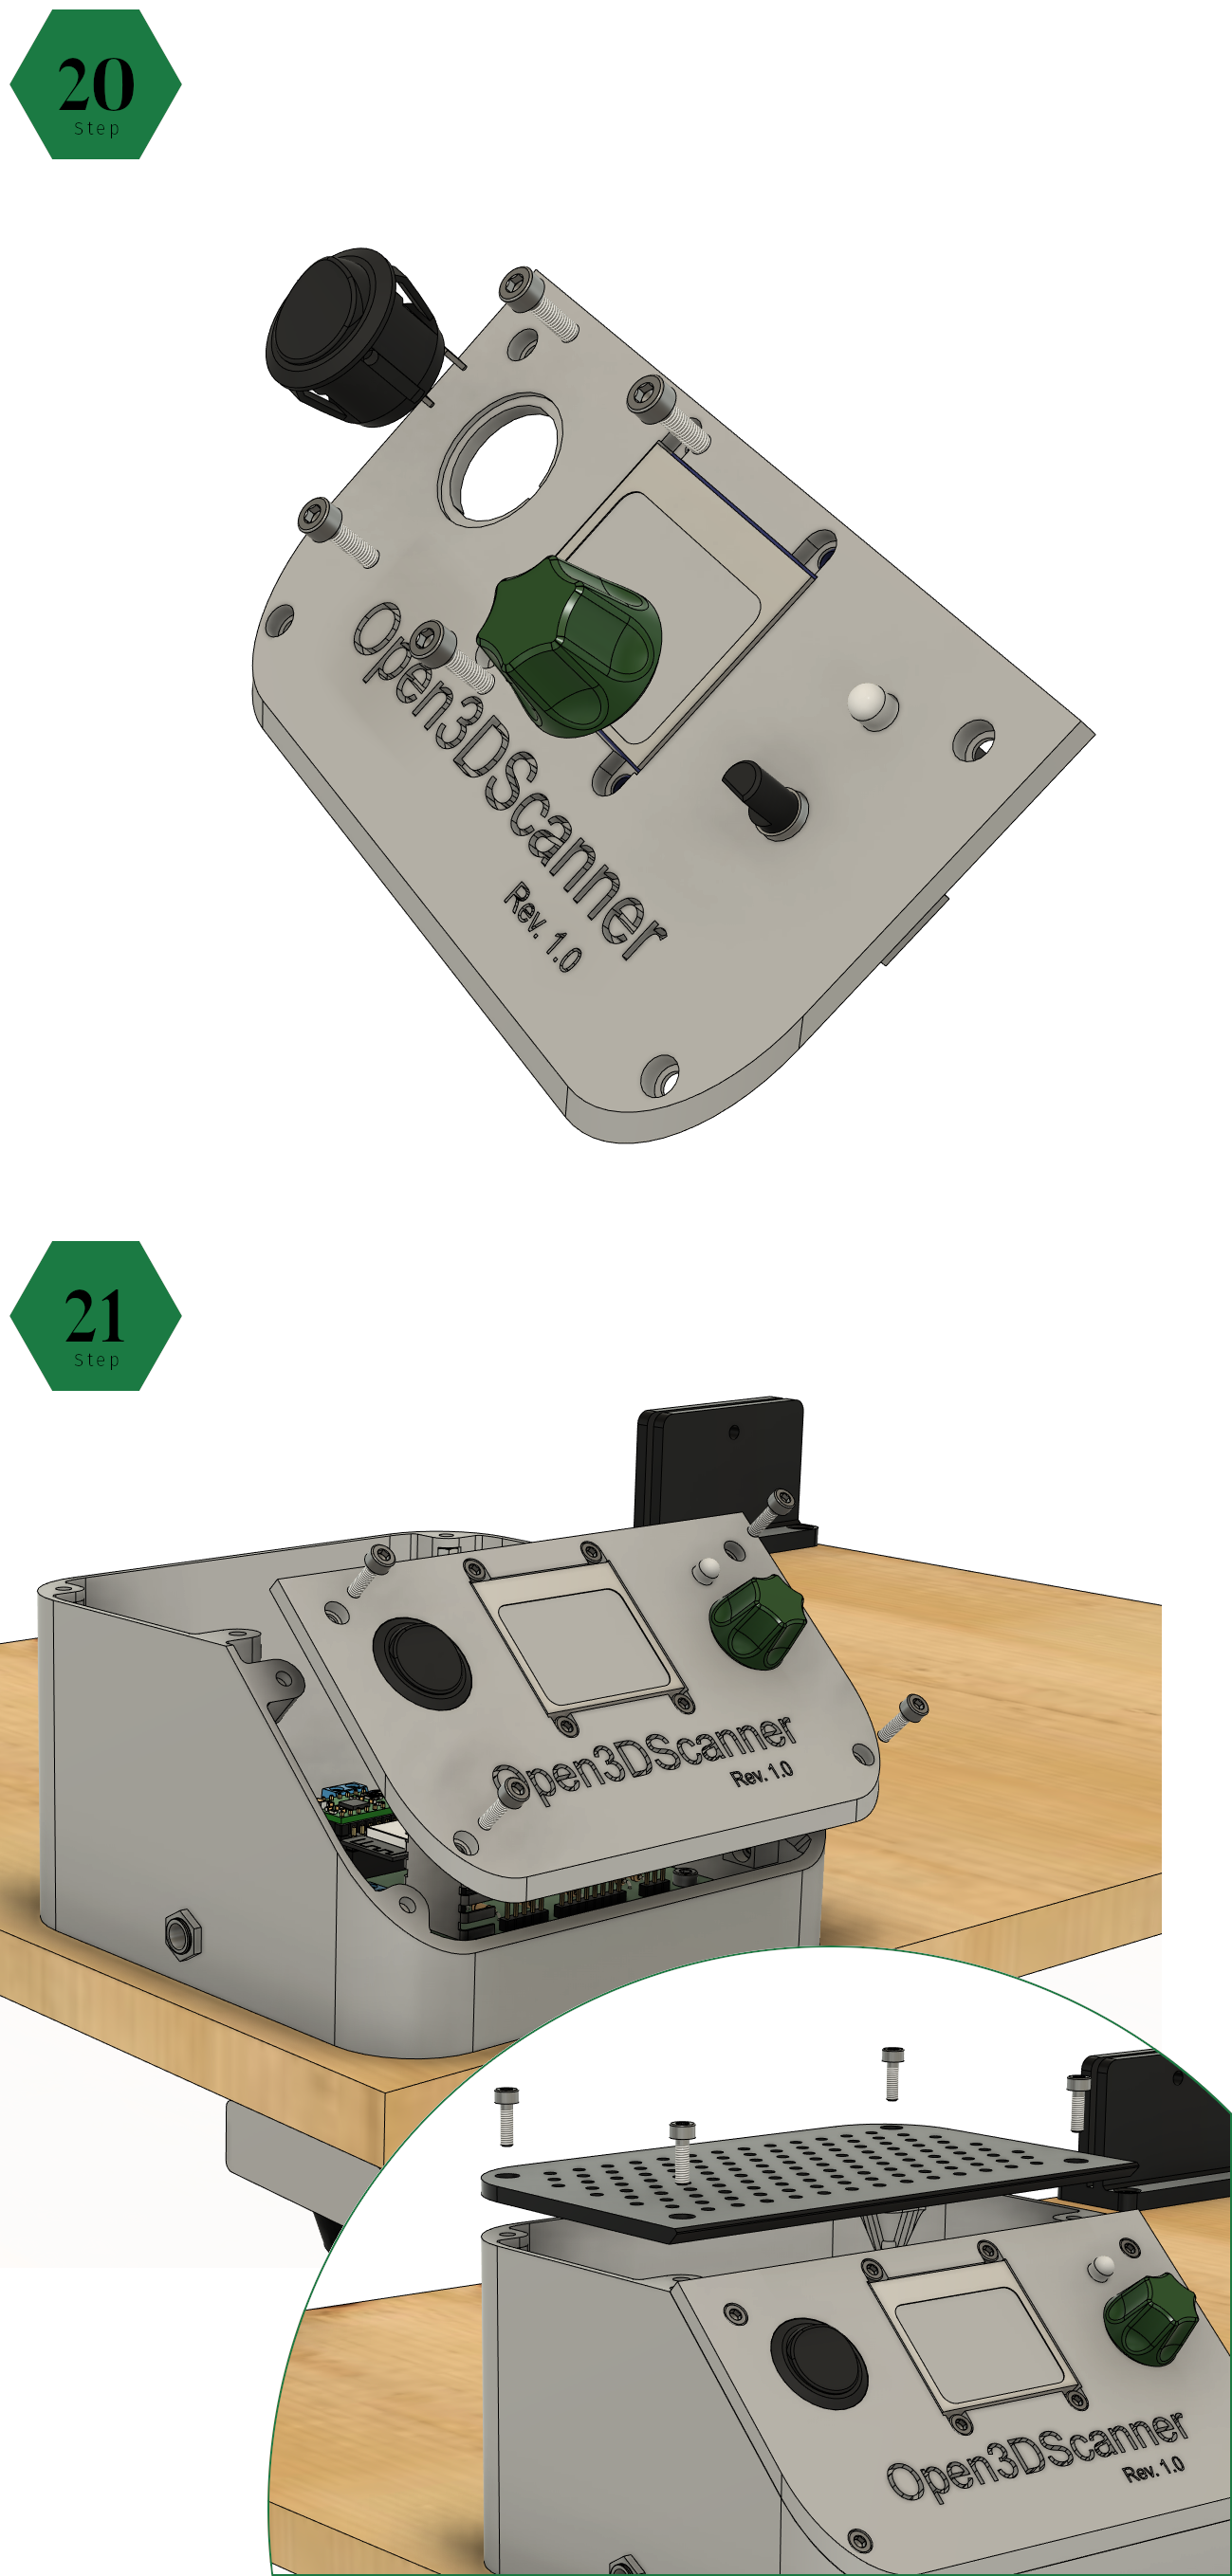
\includegraphics{images/Assembly15.png}%
{\captionof{figure}{Step 20 \& 21 of the Open3DScanner assembly}}
\clearpage%

% STEP 22 & 23
\sideTabularx[Required parts for step 22]{%
	\rowcolors{2}{tableLineTwo}{tableLineOne}% specify rowcolors in tabularx style
	\begin{tabularx} {\marginparwidth} {>{\rowmac \hsize=1.5\hsize}X>{\rowmac \hsize=0.5\hsize}X<{\clearrow}}%
		\tabularxHeader%
		Part & Quantity\\%
		4.0$\times$16 Countersunk Wood Screwt & 6\\%
	\end{tabularx}%
}%

\marginInfo*[Instructions]{Screw the assembled scanner onto the base plate.}%

\marginTips*[Tip]{For the exact alignment on the base plate, there is a detailed illustration at the end of the assembly instructions.}%

\sideTabularx[Required parts for step 23]{%
	\vspace{3.30cm}%
	\rowcolors{2}{tableLineTwo}{tableLineOne}% specify rowcolors in tabularx style
	\begin{tabularx} {\marginparwidth} {>{\rowmac \hsize=1.5\hsize}X>{\rowmac \hsize=0.5\hsize}X<{\clearrow}}%
		\tabularxHeader%
		Part & Quantity\\%
		4.0$\times$16 Countersunk Wood Screwt & 6\\%
	\end{tabularx}%
}%

\marginInfo*[Instructions]{Screw the assembled lights onto the base plate.}%

\marginTips*[Tip]{For the exact alignment on the base plate, there is a detailed illustration at the end of the assembly instructions.}%

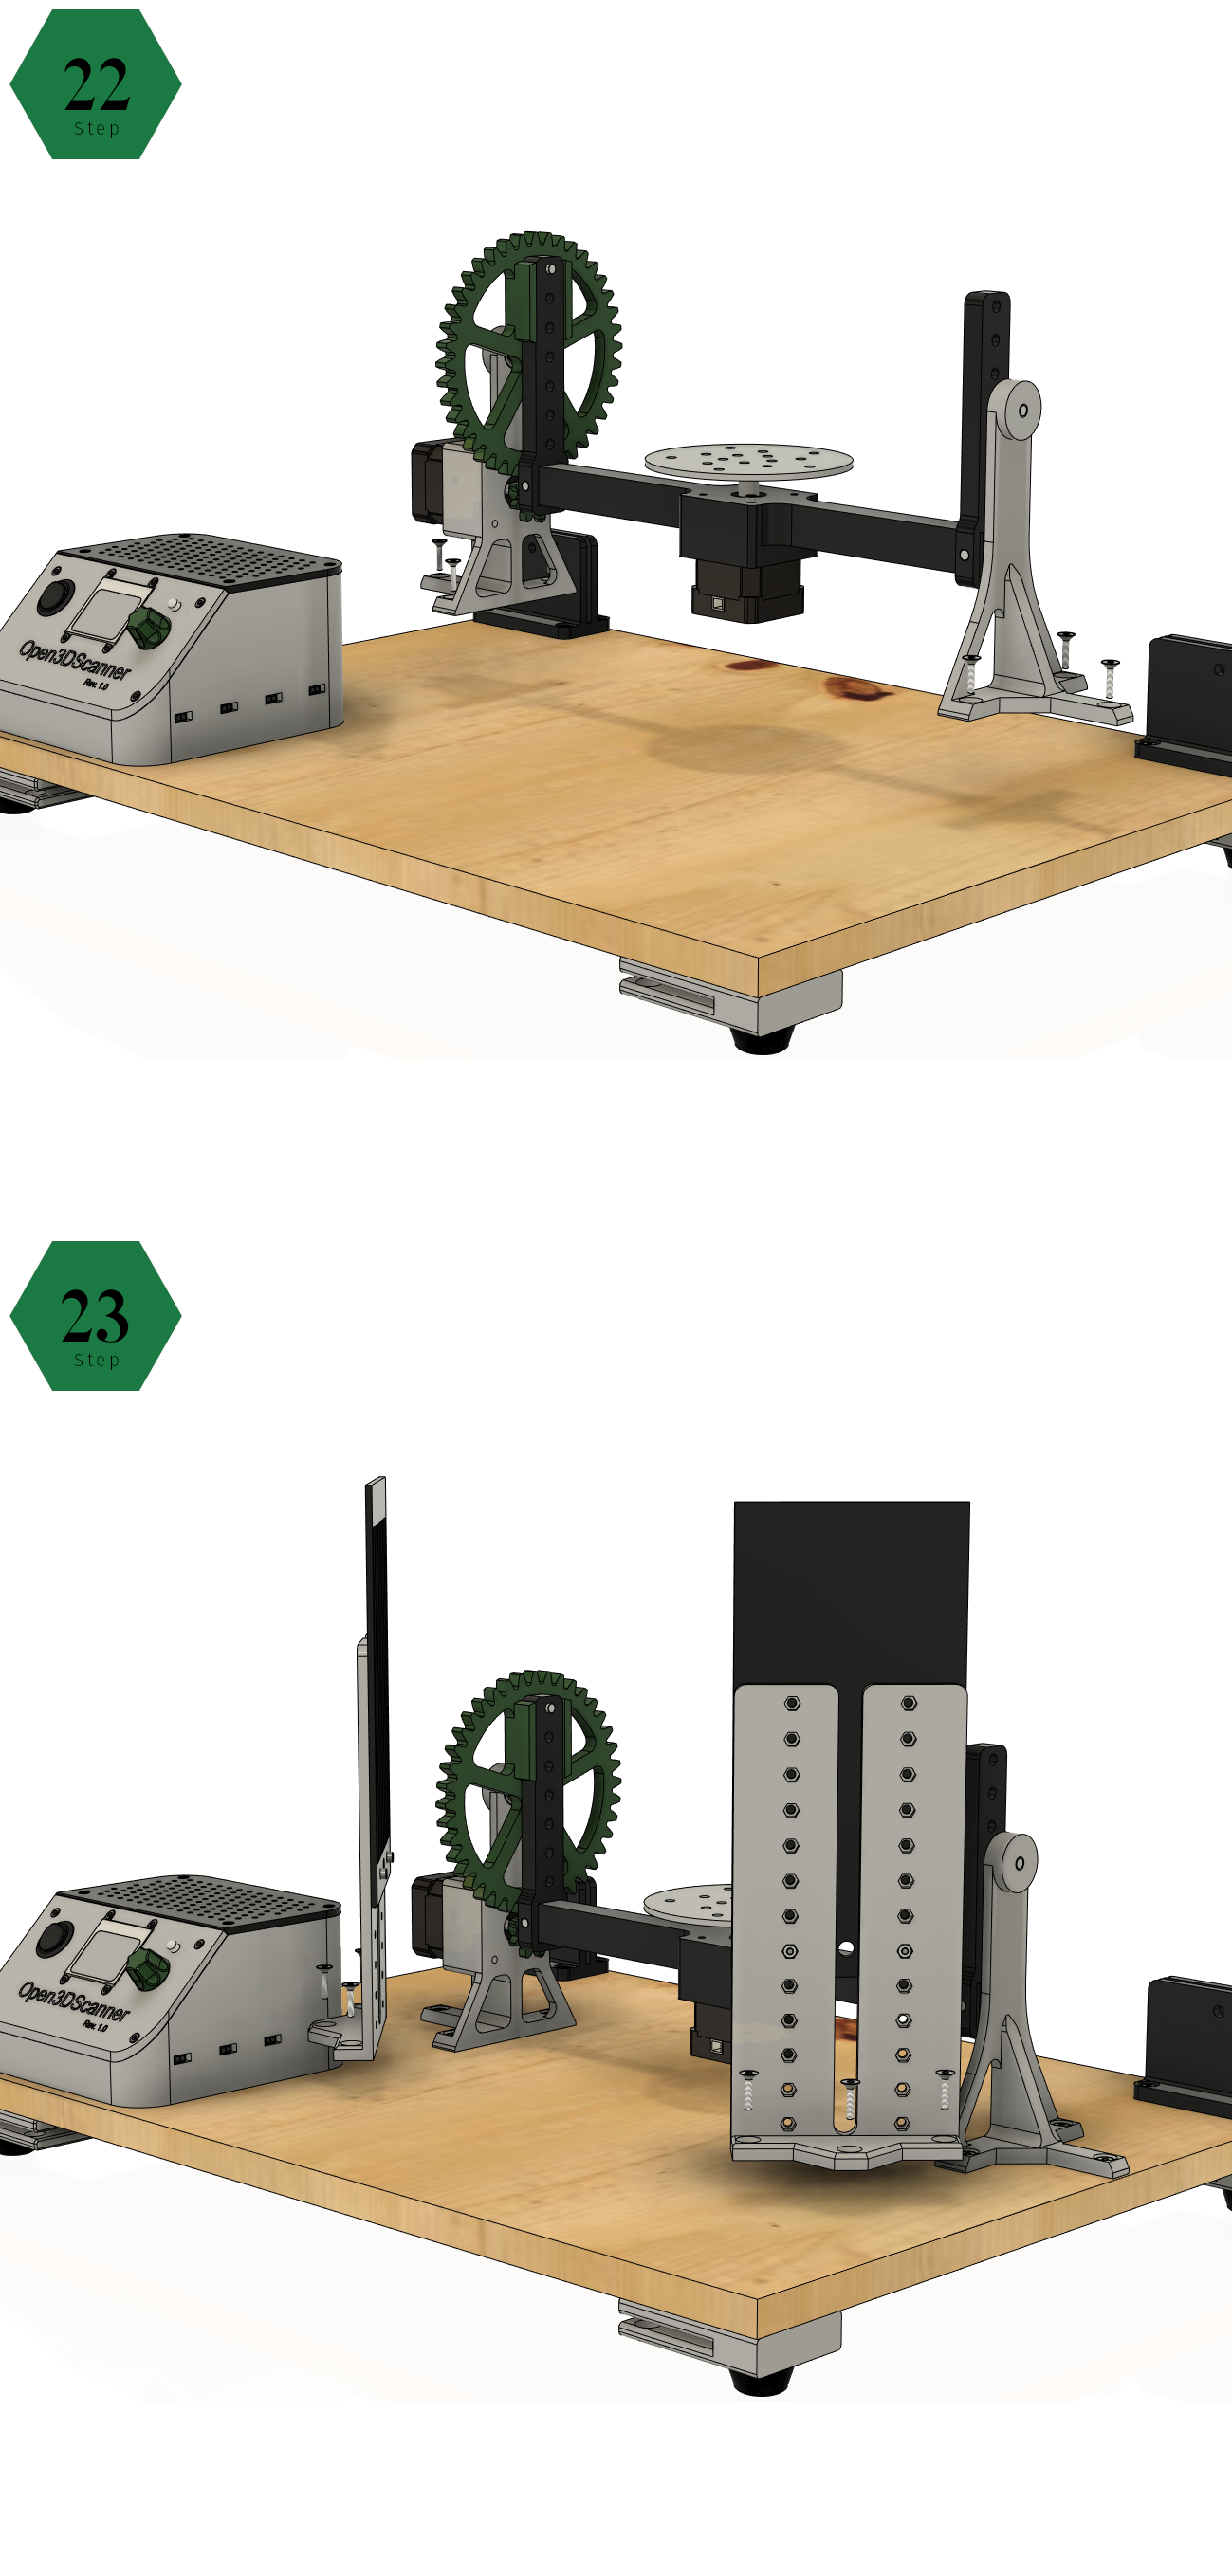
\includegraphics{images/Assembly16.png}%
{\captionof{figure}{Step 22 \& 23 of the Open3DScanner assembly}}
\clearpage%

% STEP 24 & Fin
\sideTabularx[Required parts for step 24]{%
	\rowcolors{2}{tableLineTwo}{tableLineOne}% specify rowcolors in tabularx style
	\begin{tabularx} {\marginparwidth} {>{\rowmac \hsize=1.5\hsize}X>{\rowmac \hsize=0.5\hsize}X<{\clearrow}}%
		\tabularxHeader%
		Part & Quantity\\%
		Cable-Holder & 5\\%
		4.0$\times$16 Countersunk Wood Screwt & 10\\%
	\end{tabularx}%
}%

\marginInfo*[Instructions]{Screw the cable holders onto the base plate.}%

\marginTips*[Tip]{For the exact alignment on the base plate, there is a detailed illustration at the end of the assembly instructions. All cables have to be routed for this step.}%

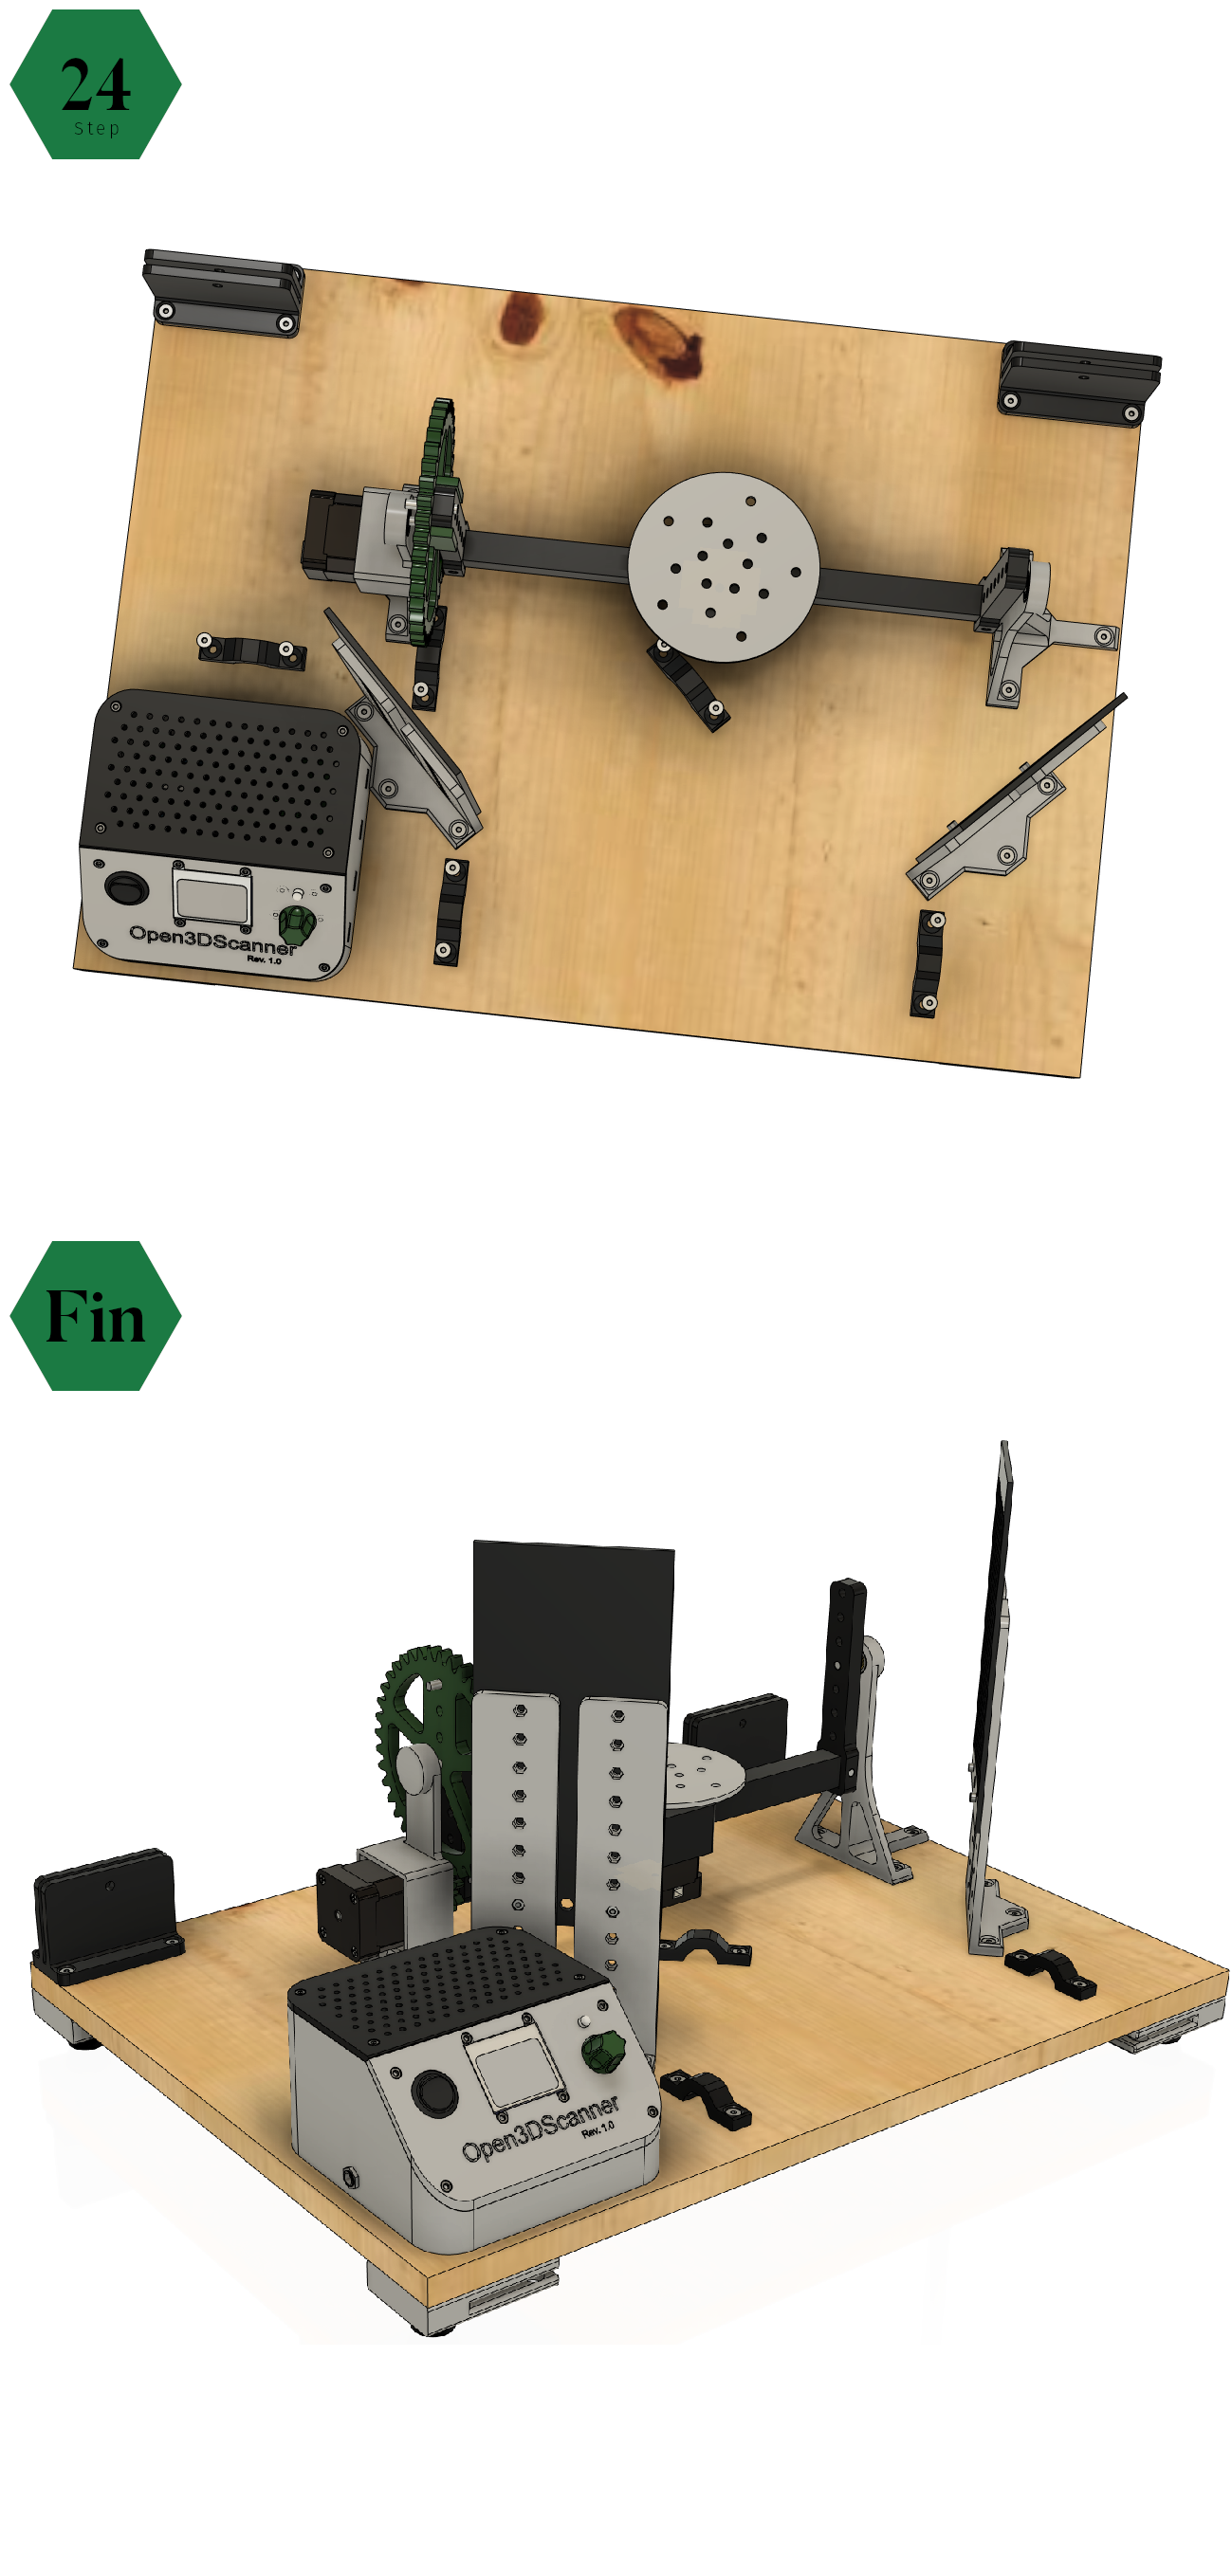
\includegraphics{images/Assembly17.png}%
{\captionof{figure}{Step 24 \& Fin of the Open3DScanner assembly}}
\clearpage%

% ALIGNMENT


\marginTips*[Tip]{This illustration is an aid for aligning the components on the base plate. All values are given in millimeters. For the individual setup, the values can deviate slightly, especially the distance between the two stands of the 3D scanner. This is due to the fact that a certain tolerance is given by the steel bars. Figure B shows the dimensions of the back plate.}%

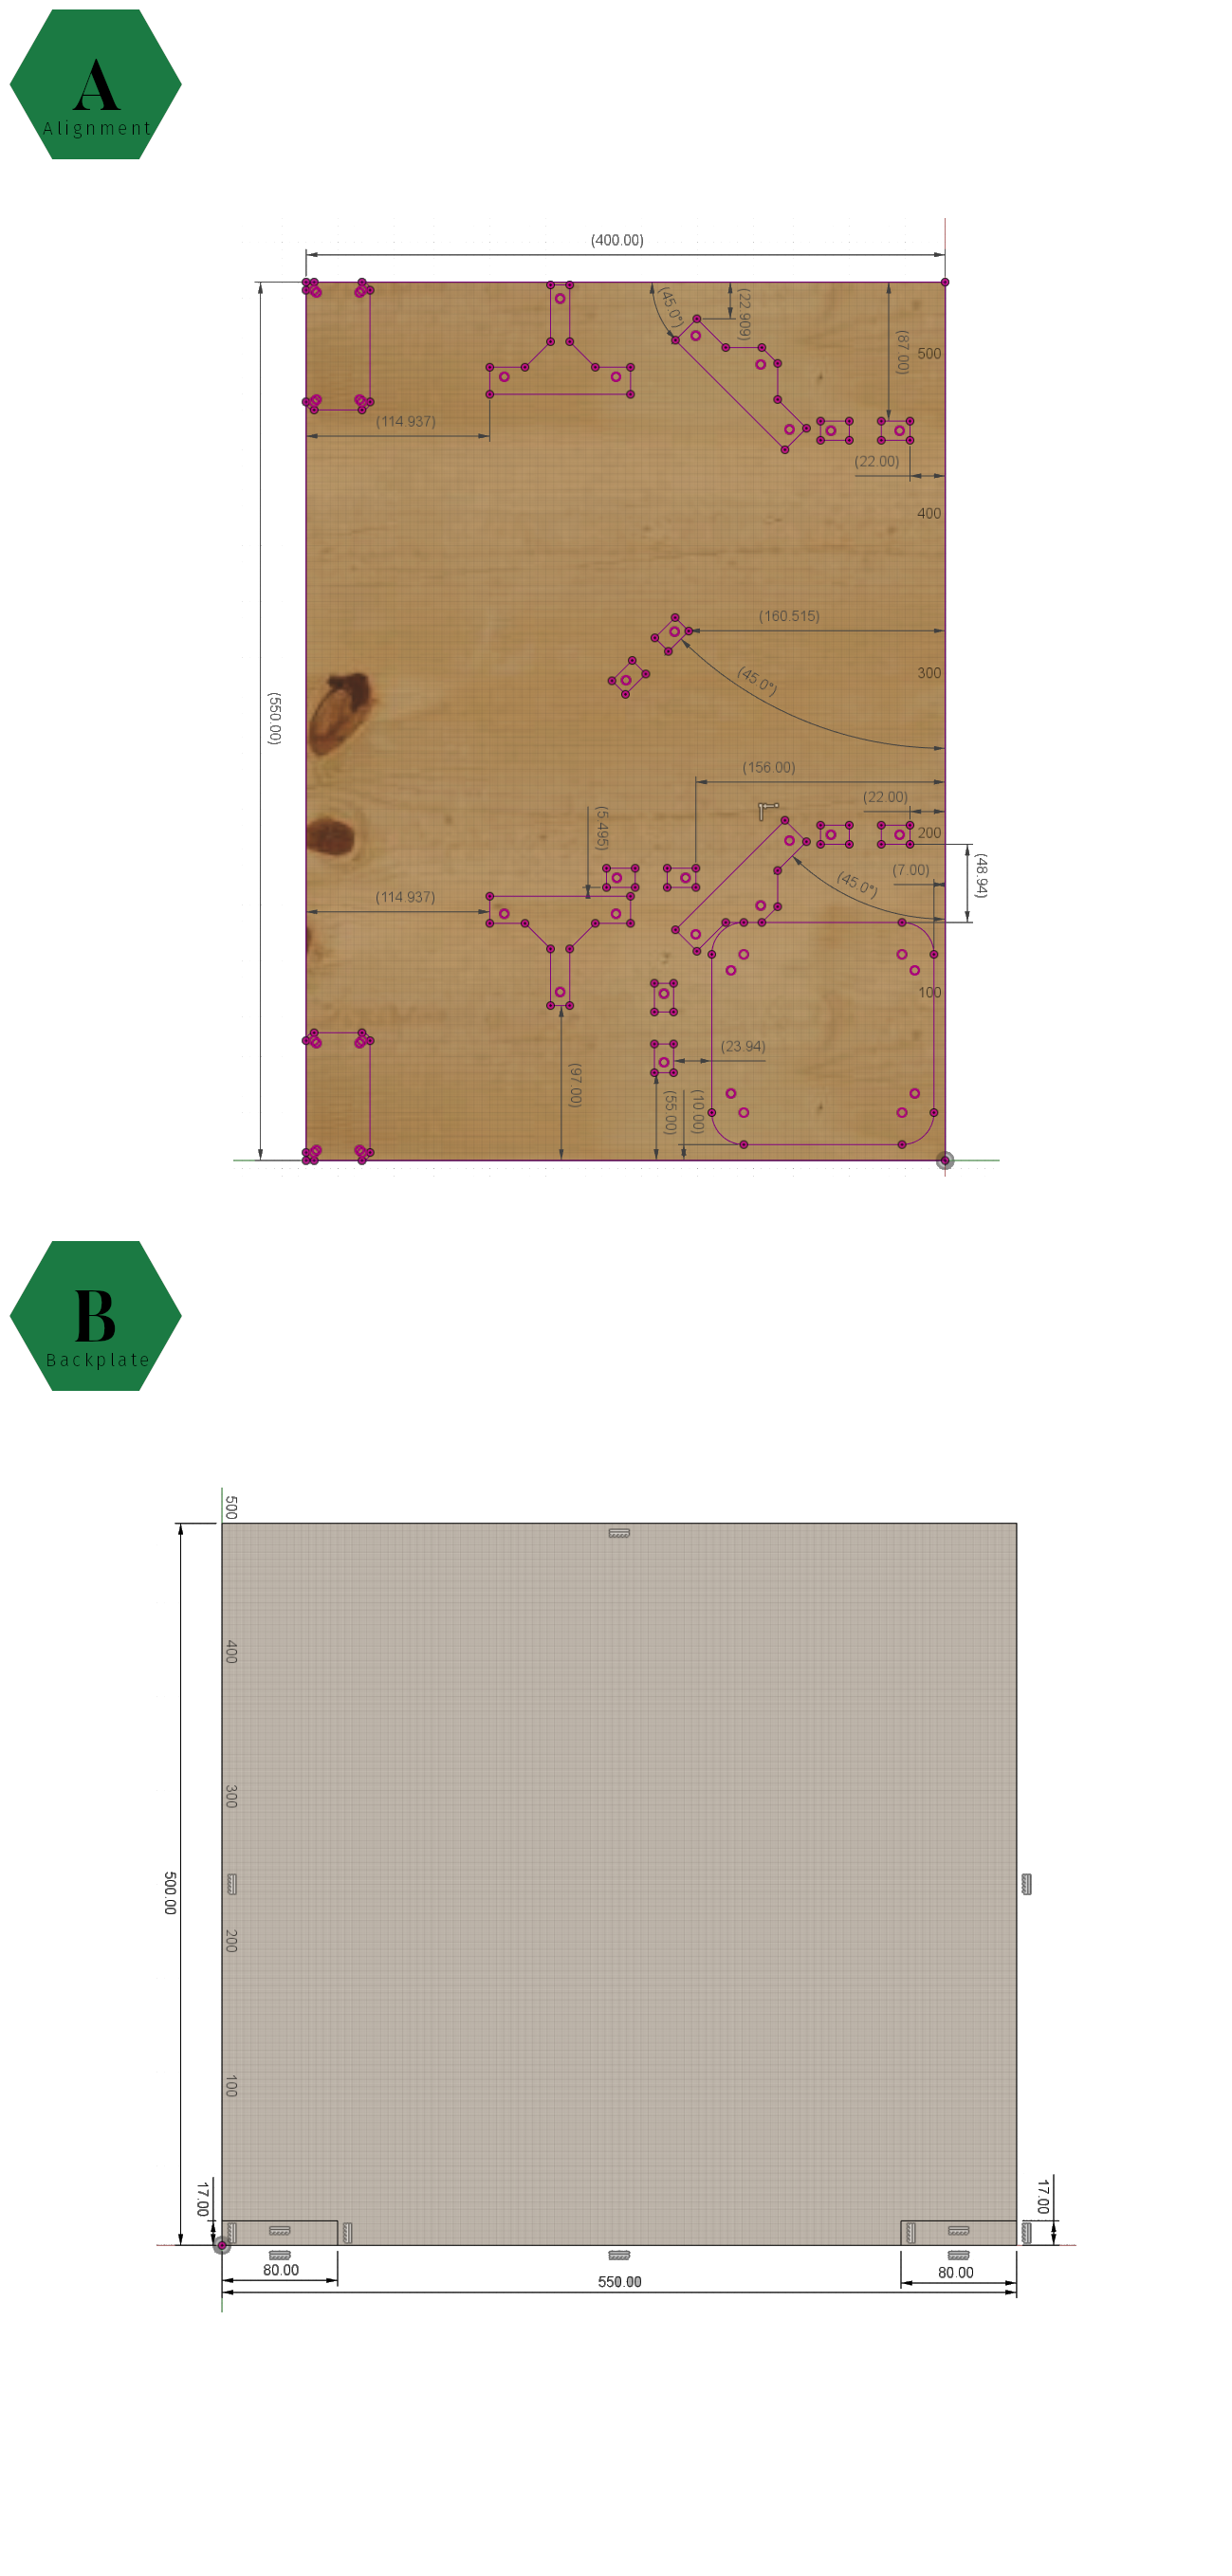
\includegraphics{images/Assembly18.png}%
{\captionof{figure}{Component Alignment on Base Plate \& Back Plate Size}}
\clearpage%%
	\chapter{User Guide}
\label{c:userGuide}
This chapter describes how to use the fully assembled Open3D scanner to create 3D scans. First, the menu navigation of the Open3DScanner is explained and then the handling of the hardware.%

\section{Menu Navigation}%
If the Open3DScanner is switched on, the user sees the main menu on the display. It contains three sub-items which lead to the menus described in the following sections. The navigation within the menu is done by the knob to the right of the display. If it is rotated, the cursor position changes or the currently selected value is changed. To confirm a selection, press the knob.%

\subsection{Scan}%
The user has two options for starting a scan: Using a preset or creating a custom scan.%

The presets are predefined scan settings that allow a quick and easy start of the scan.%

If a custom scan is selected, the user must successively specify a series of settings that define the characteristics of the subsequent scan. The selected values are persisted and selected as default values for the next custom scan. This is done under the assumption that similar scans are frequently performed.%

First, the user must determine how many images are to be taken each time the turntable on which the object to be scanned is mounted is rotated. Any value between 1 and 3200 (inclusive) can be used. 3200 corresponds to the maximum resolution of the stepper motors at 200 steps per revolution and 1/16 microstepping.%

The next step is to select how far the turntable and the object are to be rotated on the x-axis during the scan. Any value between 1 and 359 (incluseive) degrees can be selected\marginInfo[Reasonable Values]{Even if there is a large range of values for the user to choose from, it often makes little sense to rotate the object further than 180 degrees around the x-axis. I usually use values in the range of 45 and 135.}.%

Finally, the number of steps in which the rotation on the x-axis is divided must be selected. Each step corresponds to a complete rotation of the turntable with the initially selected number of steps. The value range always starts at 1 and has a maximum value that corresponds to the maximum resolution of the stepper motor for the previously selected rotation around the x-axis.%

After all these parameters have been selected, the user is presented with a summary containing all selected values, the resulting number of images and the duration of the scan. At this point the scan can either be confirmed or aborted. When a preset is selected, the summary is presented directly to the user.%

Before the actual scan is started, it must be selected whether the lights of the Open3DScanner are to be switched on or off during the scan. The user is now prompted via the display to position the used smartphone appropriately and (if not already done) to establish a Bluetooth connection with the scanner. The scan cannot be started until the necessary Bluetooth connection has been established. As soon as this has been done, the Turntable can be moved to the desired start position and the scan can be started via the knob.%

During scanning, the current progress is shown on the display. It shows the number of recorded images, their total number and the remaining time. If the Bluetooth connection to the smartphone is lost during the scan, the scan is interrupted and the user is prompted to re-establish the connection. If the knob is pressed during the scan, the scan can be aborted or resumed after confirmation.%

\subsection{Settings}%
The settings menu is divided into categories that group the individual settings.%

\subsubsection{Scan}%
In this setting menu, you can set how many milliseconds the scanner stops after a motor movement or after taking a photo. This is necessary to allow the camera to focus images, but also to prevent possible vibrations of the scanner from blurring the images.%

\subsubsection{Display}%
In addition to the option of switching the backlight for the display on or off, the contrast of the display can be adjusted here.%

\subsubsection{Camera}%
Here you can select which camera type will be used during the scan. This is important because the control of various devices is different. Currently iOs and Android devices are supported.%

\subsubsection{Steppers}%
This menu allows you to adjust the behavior of the stepper motors. The selected stepper motor moves 15° back and forth while the settings are adjusted. This makes changes directly visible.%

The direction of movement of the motors can be changed if necessary. In addition, it can be determined with how many RPM the motor should move, what the acceleration and deceleration curve should look like, and which maximum values should be used for acceleration and deceleration.%

\subsection{Debug}%
The debug menu contains options to test some features of the Open3DScanner. Currently it is possible to switch the connected lights on and off and to trigger the camera. The system does not check whether a Bluetooth connection is actually present, so this must be checked in advance on the connected device.%

\section{Hardware Handling}%
This section contains some information about the built scanner and the interaction with the device.%

\subsection{Object Mounting}%
For the scan it is necessary to attach the object to be scanned to the Turntable. The holes in the Turntable allow to fix the object with cable ties. But this can lead to artefacts in the scan, so I prefer to use adhesive putty which can be reused many times.%

\subsection{Scanner Adjustment}%
Depending on the size of the object to be scanned, it may be useful to adjust the height of the lights or the turntable. The parts have been designed to allow this. This makes it possible to move the rotation center of the x-axis near the center of the object to be scanned.%

Thus, depending on the object, it can be ensured that it is always in the field of view of the camera, which is important for the automatic creation of images.%

\subsection{Status LED}%
The Open3DScanner has a bi-color LED, which is used to indicate the state of the scanner. The different state are explained below.%

\begin{table}[ht!]%
	\begin{centered}%
		\rowcolors{2}{tableLineTwo}{tableLineOne}% specify rowcolors in tabularx style
		\begin{tabularx} {\linewidth} {>{\rowmac \hsize=1\hsize}X>{\rowmac \hsize=1\hsize}X>{\rowmac \hsize=1\hsize}X<{\clearrow}}%
			\tabularxHeader%
			LED & State & Note\\%
			The LED lights green & Running & The scanner is turned on and ready for user interaction.\\%
			The LED lights yellow & Scanning & The scanner is performing a scan.\\%
			The LED flashes green very slowly & Scan finished & A scan has been finished successfully.\\%
			The LED flashes yellow slowly & Scan will continue & An interrupted scan will be continued soon.\\%
			The LED flashes red fast & No connection & The Bluetooth connection has been lost during scanning.\\%
		\end{tabularx}%
		\caption{Different states of the status LED}%
	\end{centered}%
\end{table}%%
	\chapter{Perform Scans}
\label{c:performingScans}
Even though I am not an expert in the field of photogrammetry, I have gathered some experiences which I would like to share here. The recommendations given in this chapter do not claim to be universally valid and are based on my individual experiences.%

\section{Lighting \& Surface}%
A uniform illumination of the object to be scanned improves the quality of the scans significantly. In addition, glossy and transparent objects are much harder to scan compared to matte objects. For this reason, such objects should be treated (if possible) so that they have a better surface for the scanner. This can be done, for example, by spraying the objects with chalk spray.%

\section{Camera Settings}%
Most smartphone cameras have several features that automatically improve image quality. These range from autofocus and automatic white balance to AI functions that adjust color schemes based on recognized image content. Even if these functions provide better snapshots in everyday life, they are detrimental to the goals of photogrammetry. These functions make it more difficult to combine the images, which results in poorer scans.%

For this reason, the functions should be deactivated as far as possible and photos should be taken with fixed settings. This is especially true for color temperature, auto white balance, and autofocus.%

\section{Augmented Reconstruction}%
Since the object to be scanned must be attached to the turntable, an area of the object is always not visible on the captured images. This means that a single scan is not sufficient to scan an object completely. This may not be a problem for objects that have a flat base on which they stand and when no texture is required for that area.%

For many other objects this is a problem and multiple scans must be performed with different orientations of the object to capture the object from all sides.%

At least the software Meshroom has the function augmented reconstruction for this case. It allows to add another data set (an additional scan) to an existing data set (the first scan) and to calculate a new overall result. This can repeated as often as needed and results in a tree like structure of the Meshroom processing graph.%

That way it is often possible to create complete scans of objects. It may be necessary to filter some remaining artifacts of e.g. the Turntable of the reconstructed 3D model, but except from that you get a full scan and 3D model of the scanned object.%

This feature can also be used if the reconstructed model lacks details in some areas. Just perform an additional (detailed) scan of the respective area and start an augmented reconstruction.%%
	\appendix% start appendices
	\chapter{Picture Series PCB Assembly}%
\label{cha:picSerPCB}%

This chapter contains a series of pictures that show step by step how the individual components are soldered onto the PCB.%

The images are completely uncommented, as they are not intended as instructions, but only as a reference.%

More detailed information on assembling the circuit board can be found in section~\ref{sec:assPCB}.%

It is quite possible that individual components may look different in your case, this applies especially to resistors and heat sinks. This is not a problem as long as the components are purchased to match the BOM.%

It is possible to use the pictures to determine the order in which the individual parts are assembled. However, this is not an instruction or obligation. Assemble the parts in the order that suits you best.%

\begin{figure}[ht!]%
	\begin{centered}%
		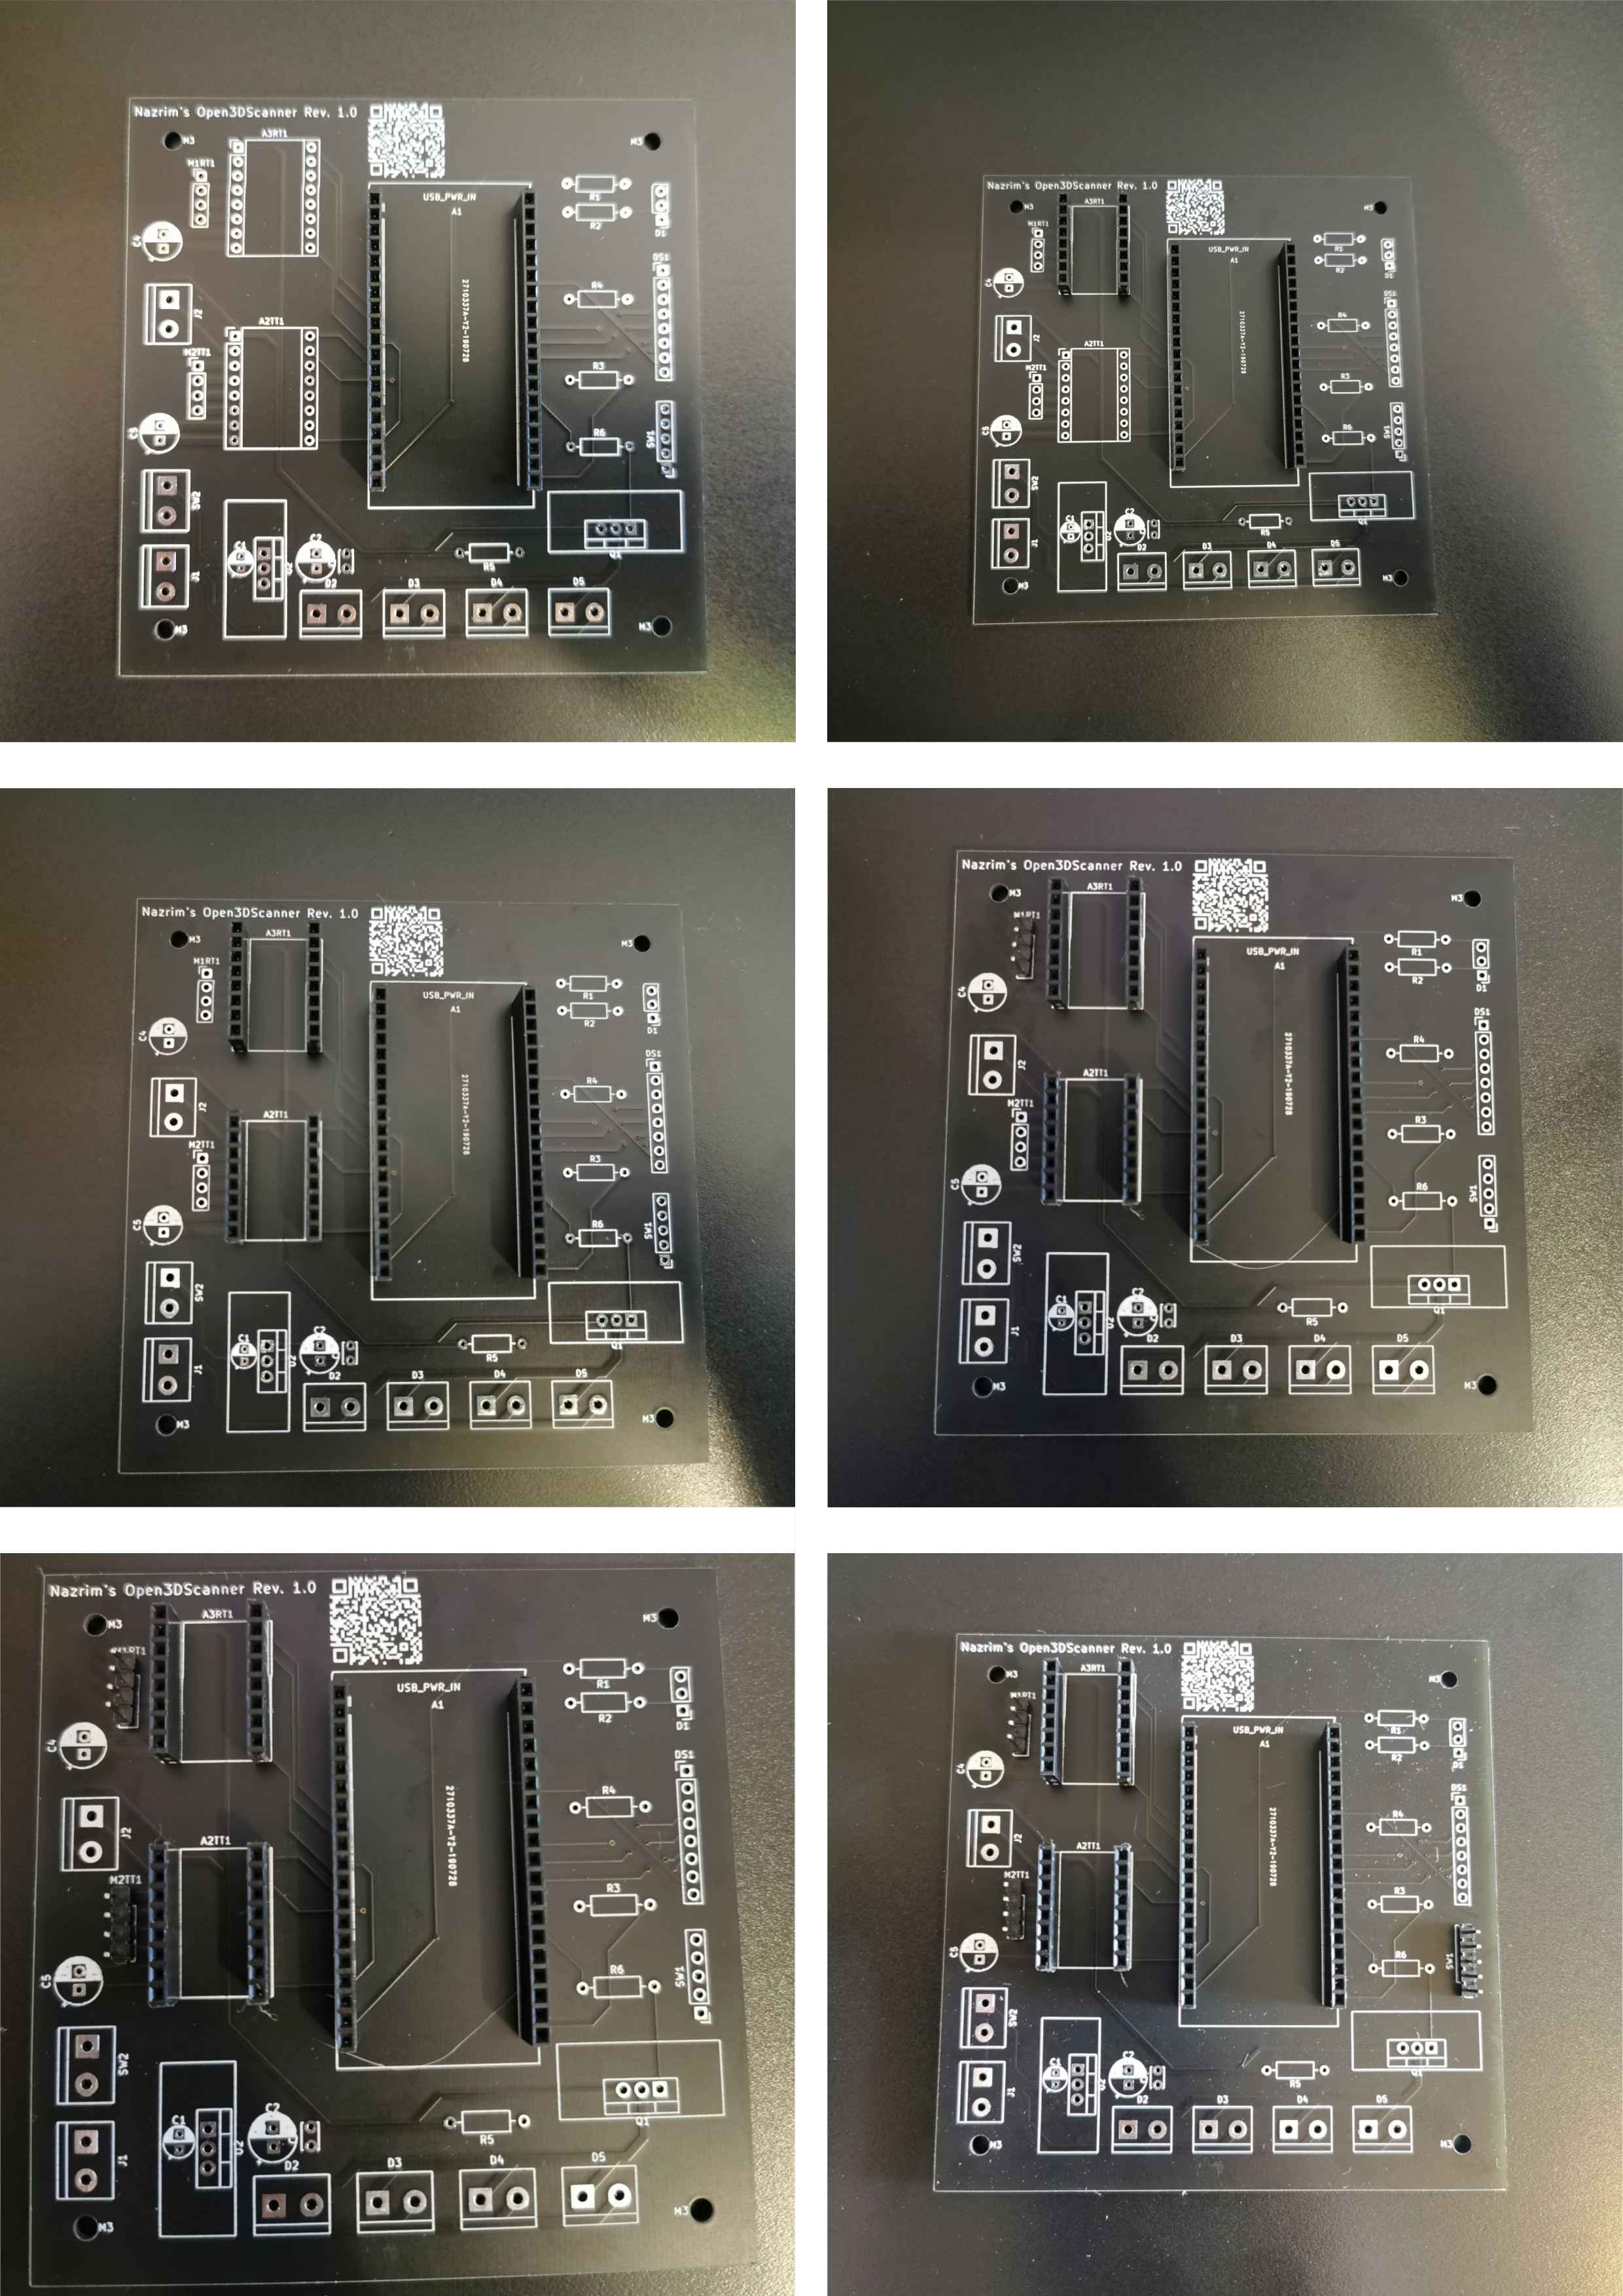
\includegraphics[width=\linewidth]{images/PcbSeries1.jpg}%
		\caption{Steps \numrange[text-rm=\lightBoldFont]{1}{6} of PCB assembly}%
	\end{centered}%
\end{figure}%

\begin{figure}[ht!]%
	\begin{centered}%
		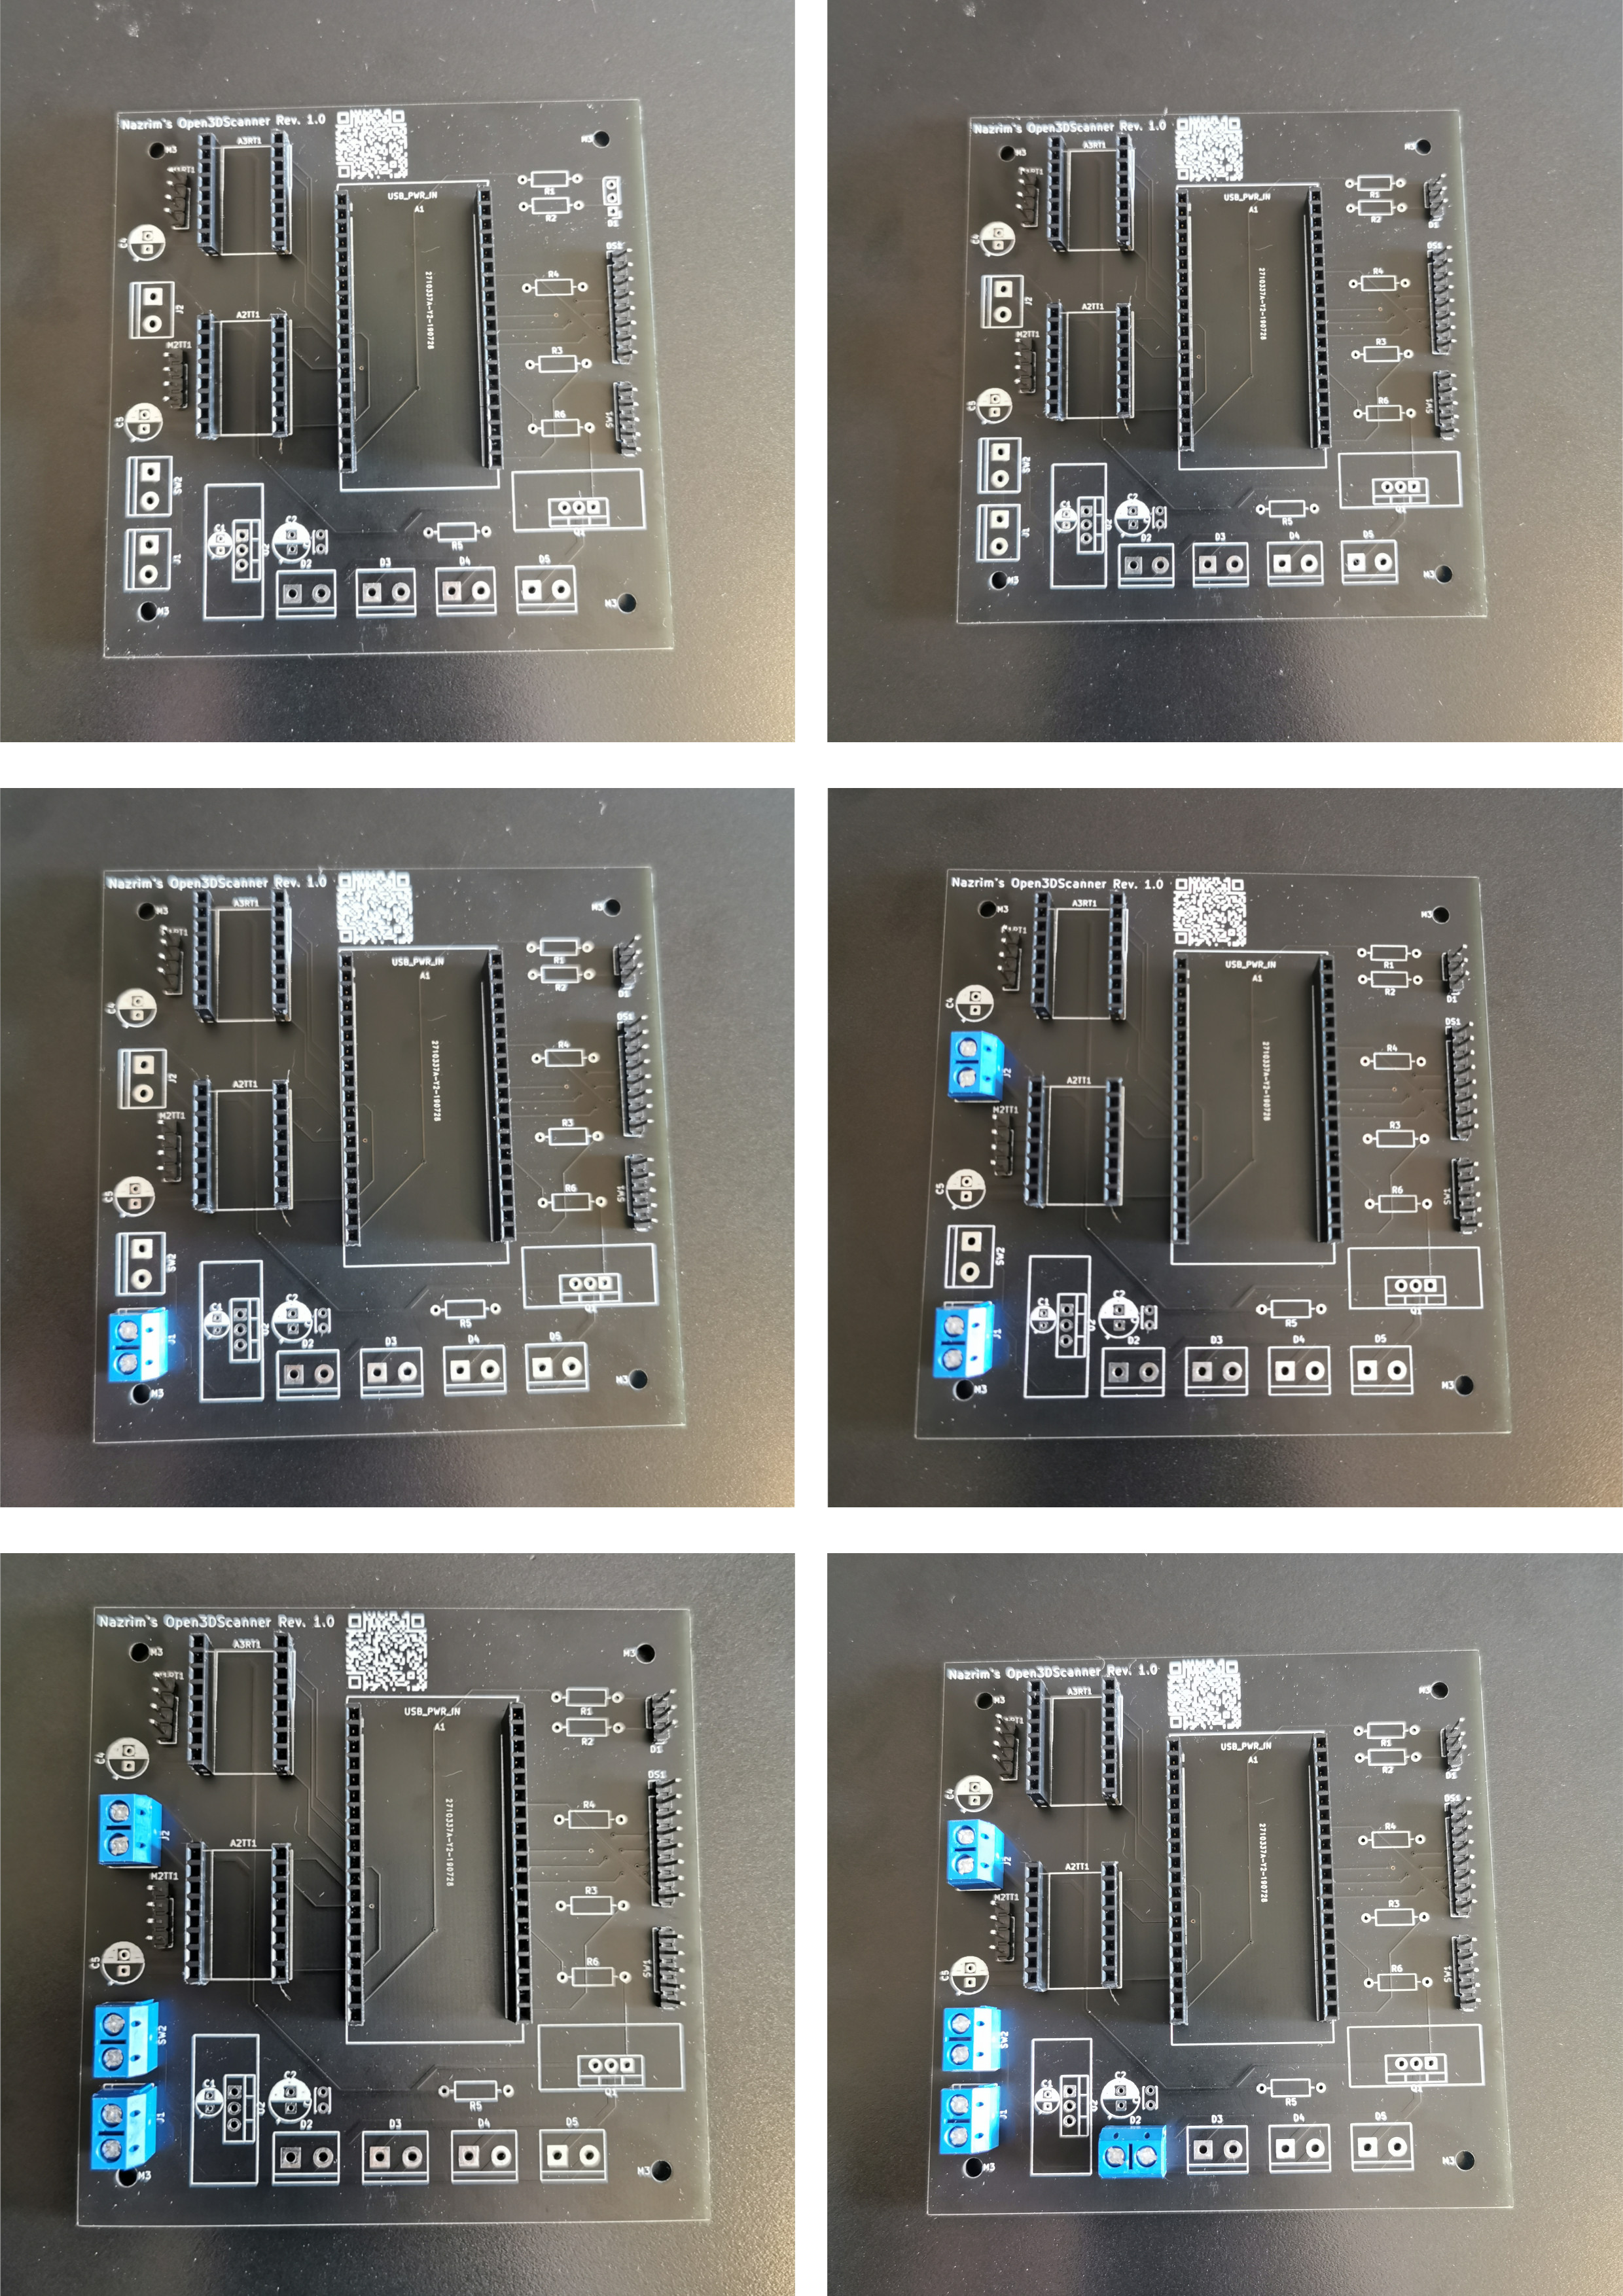
\includegraphics[width=\linewidth]{images/PcbSeries2.jpg}%
		\caption{Steps \numrange[text-rm=\lightBoldFont]{7}{12} of PCB assembly}%
	\end{centered}%
\end{figure}%

\begin{figure}[ht!]%
	\begin{centered}%
		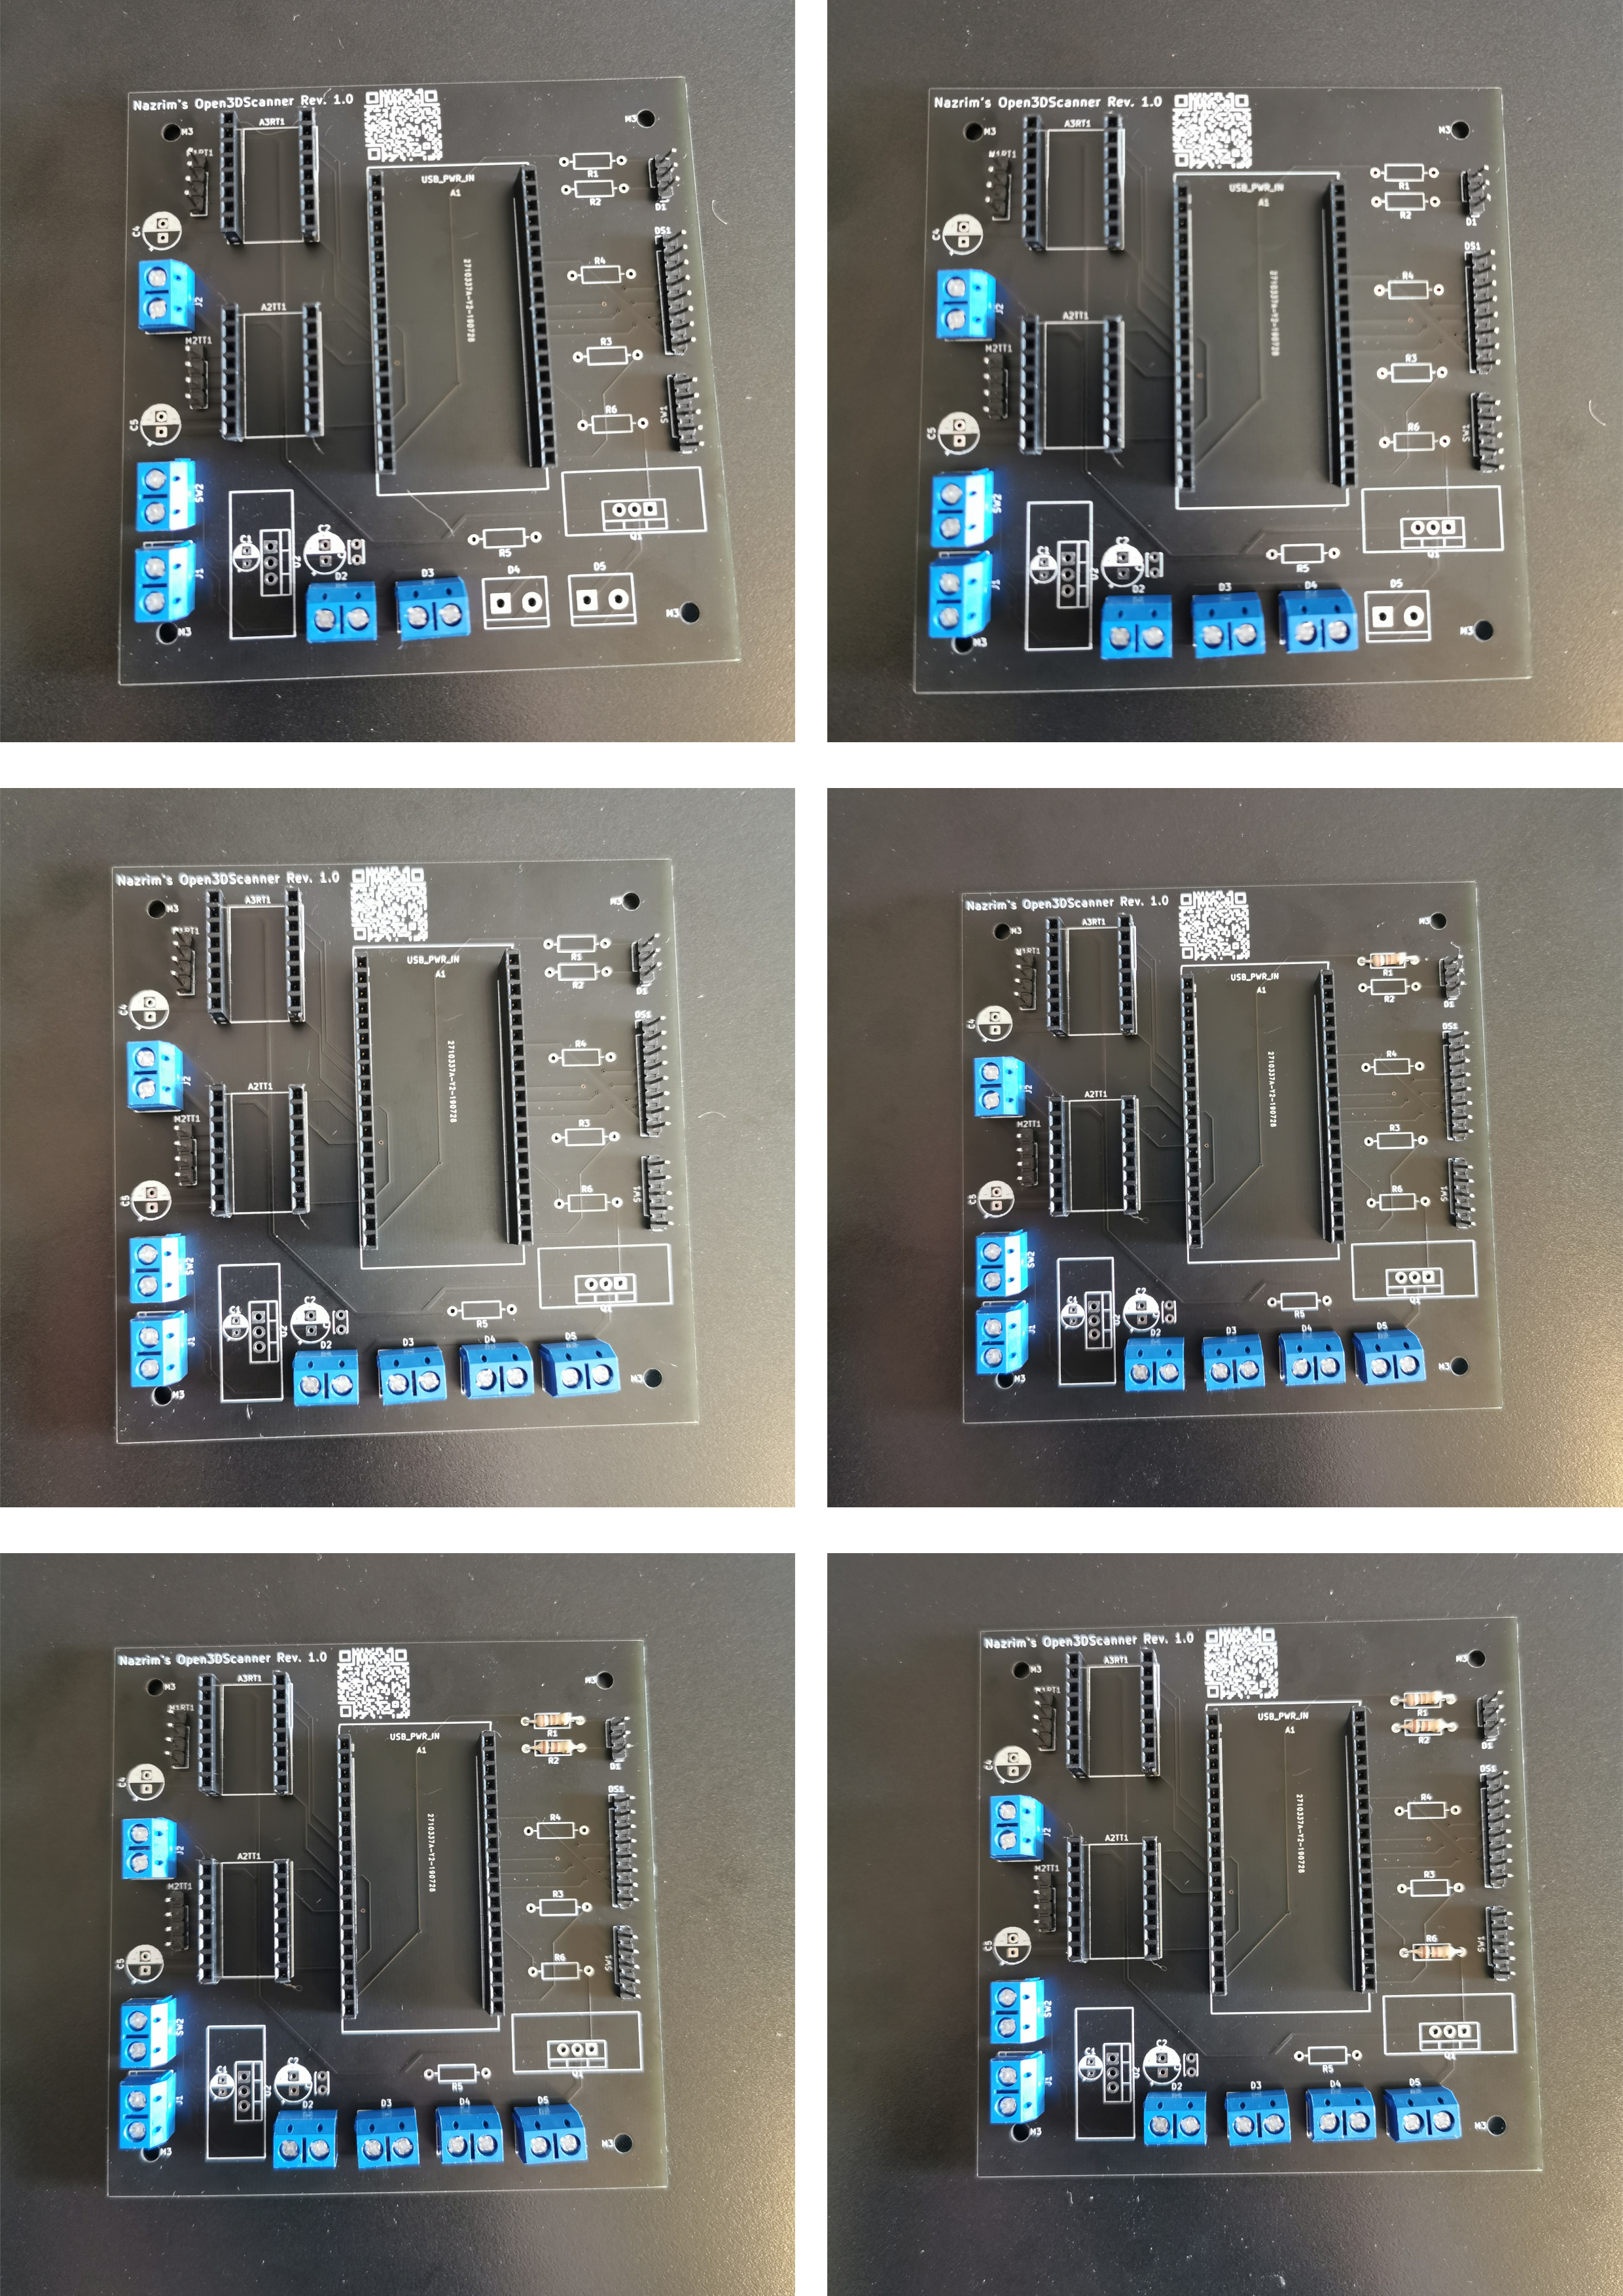
\includegraphics[width=\linewidth]{images/PcbSeries3.jpg}%
		\caption{Steps \numrange[text-rm=\lightBoldFont]{13}{18} of PCB assembly}%
	\end{centered}%
\end{figure}%

\begin{figure}[ht!]%
	\begin{centered}%
		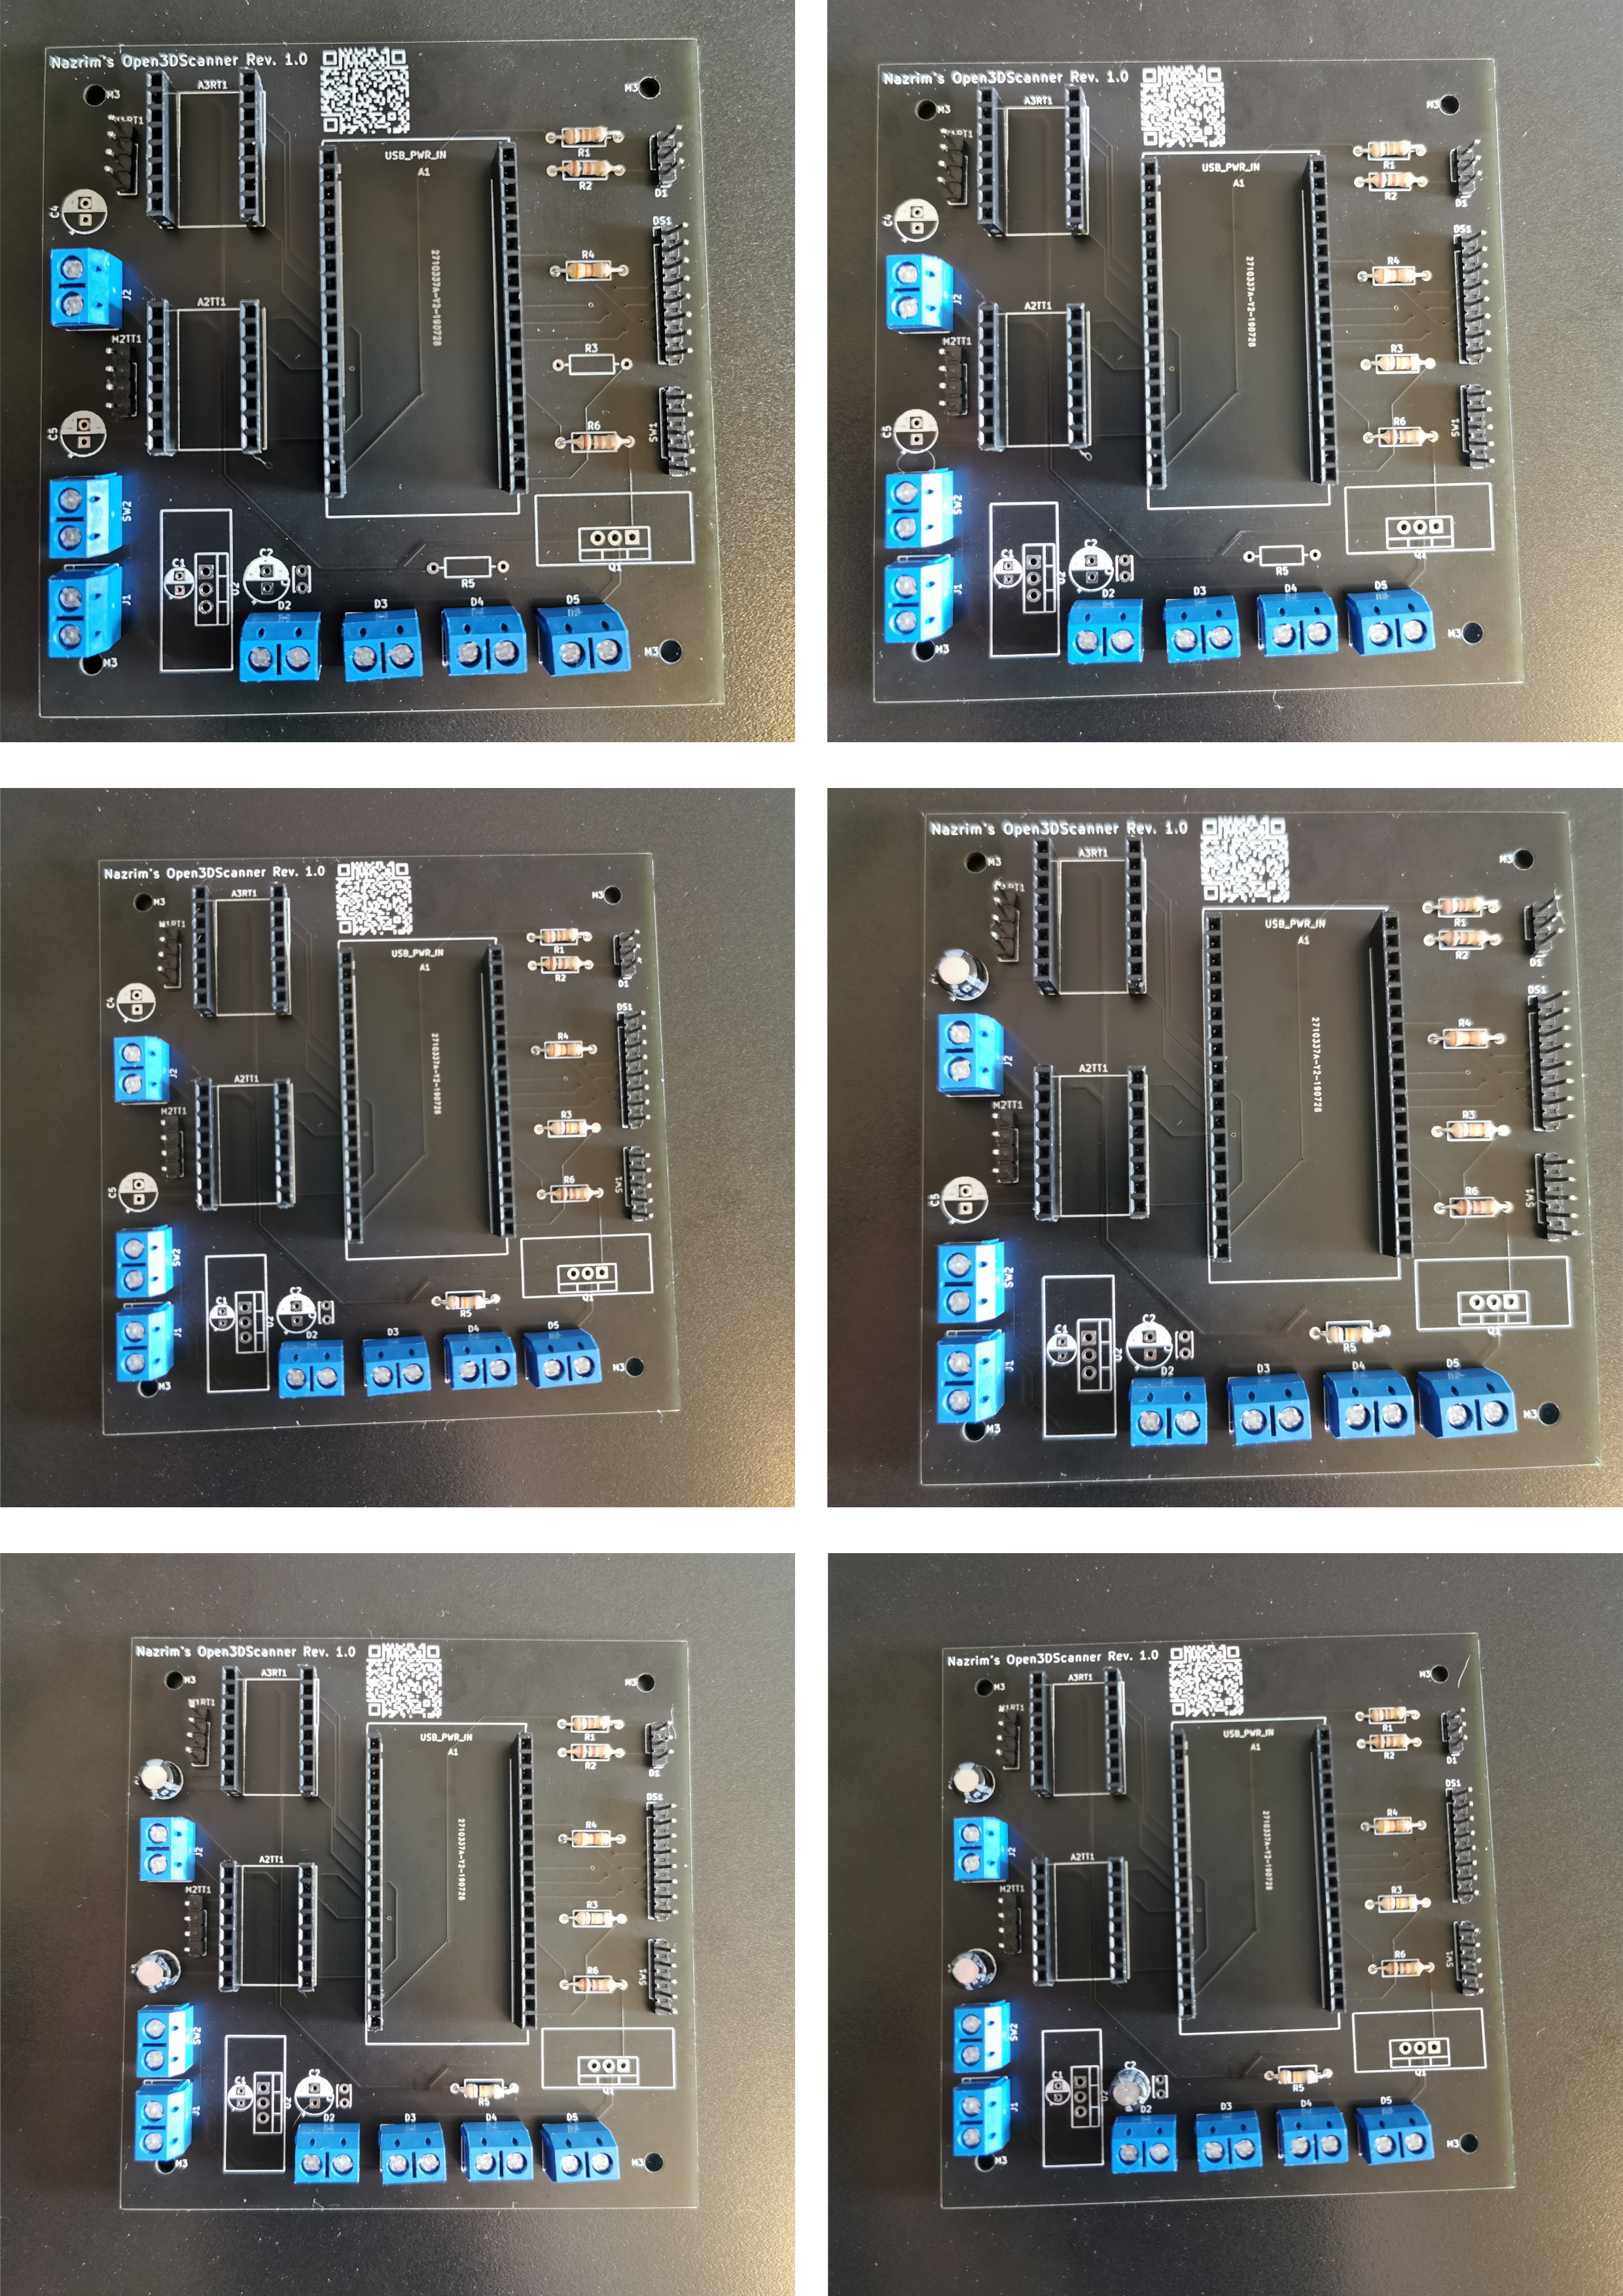
\includegraphics[width=\linewidth]{images/PcbSeries4.jpg}%
		\caption{Steps \numrange[text-rm=\lightBoldFont]{19}{24} of PCB assembly}%
	\end{centered}%
\end{figure}%

\begin{figure}[ht!]%
	\begin{centered}%
		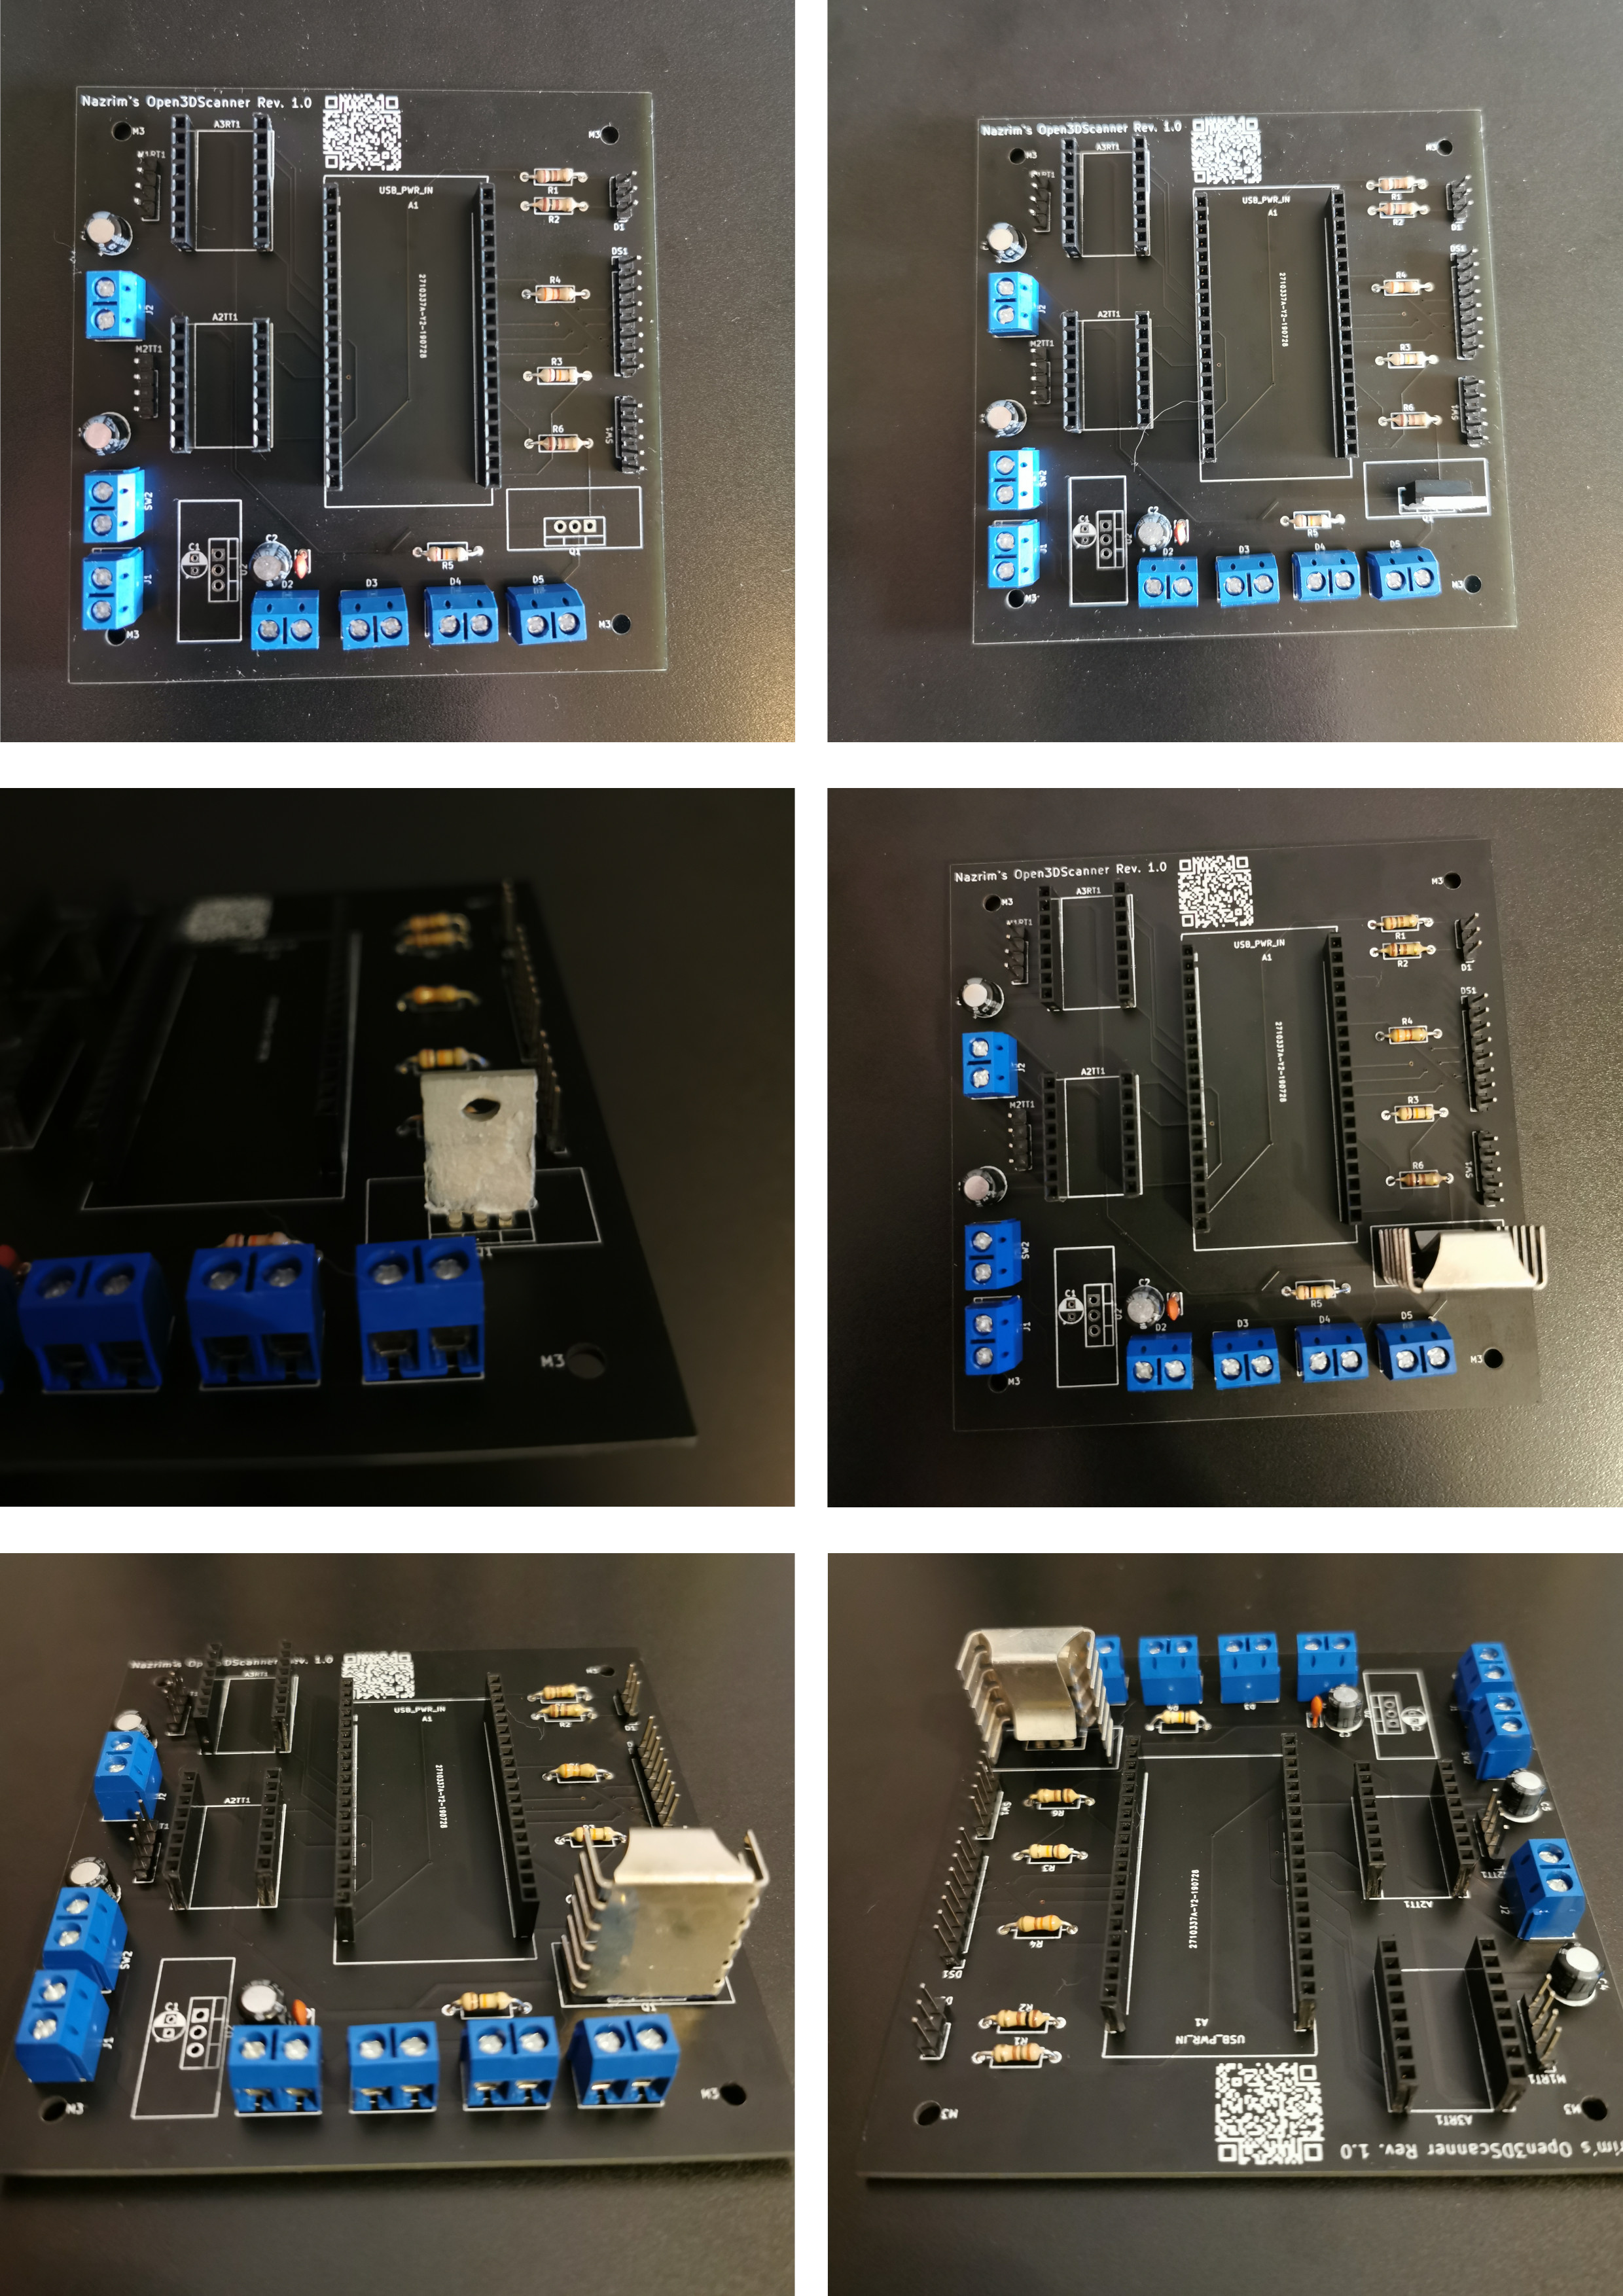
\includegraphics[width=\linewidth]{images/PcbSeries5.jpg}%
		\caption{Steps \numrange[text-rm=\lightBoldFont]{25}{30} of PCB assembly}%
	\end{centered}%
\end{figure}%

\begin{figure}[ht!]%
	\begin{centered}%
		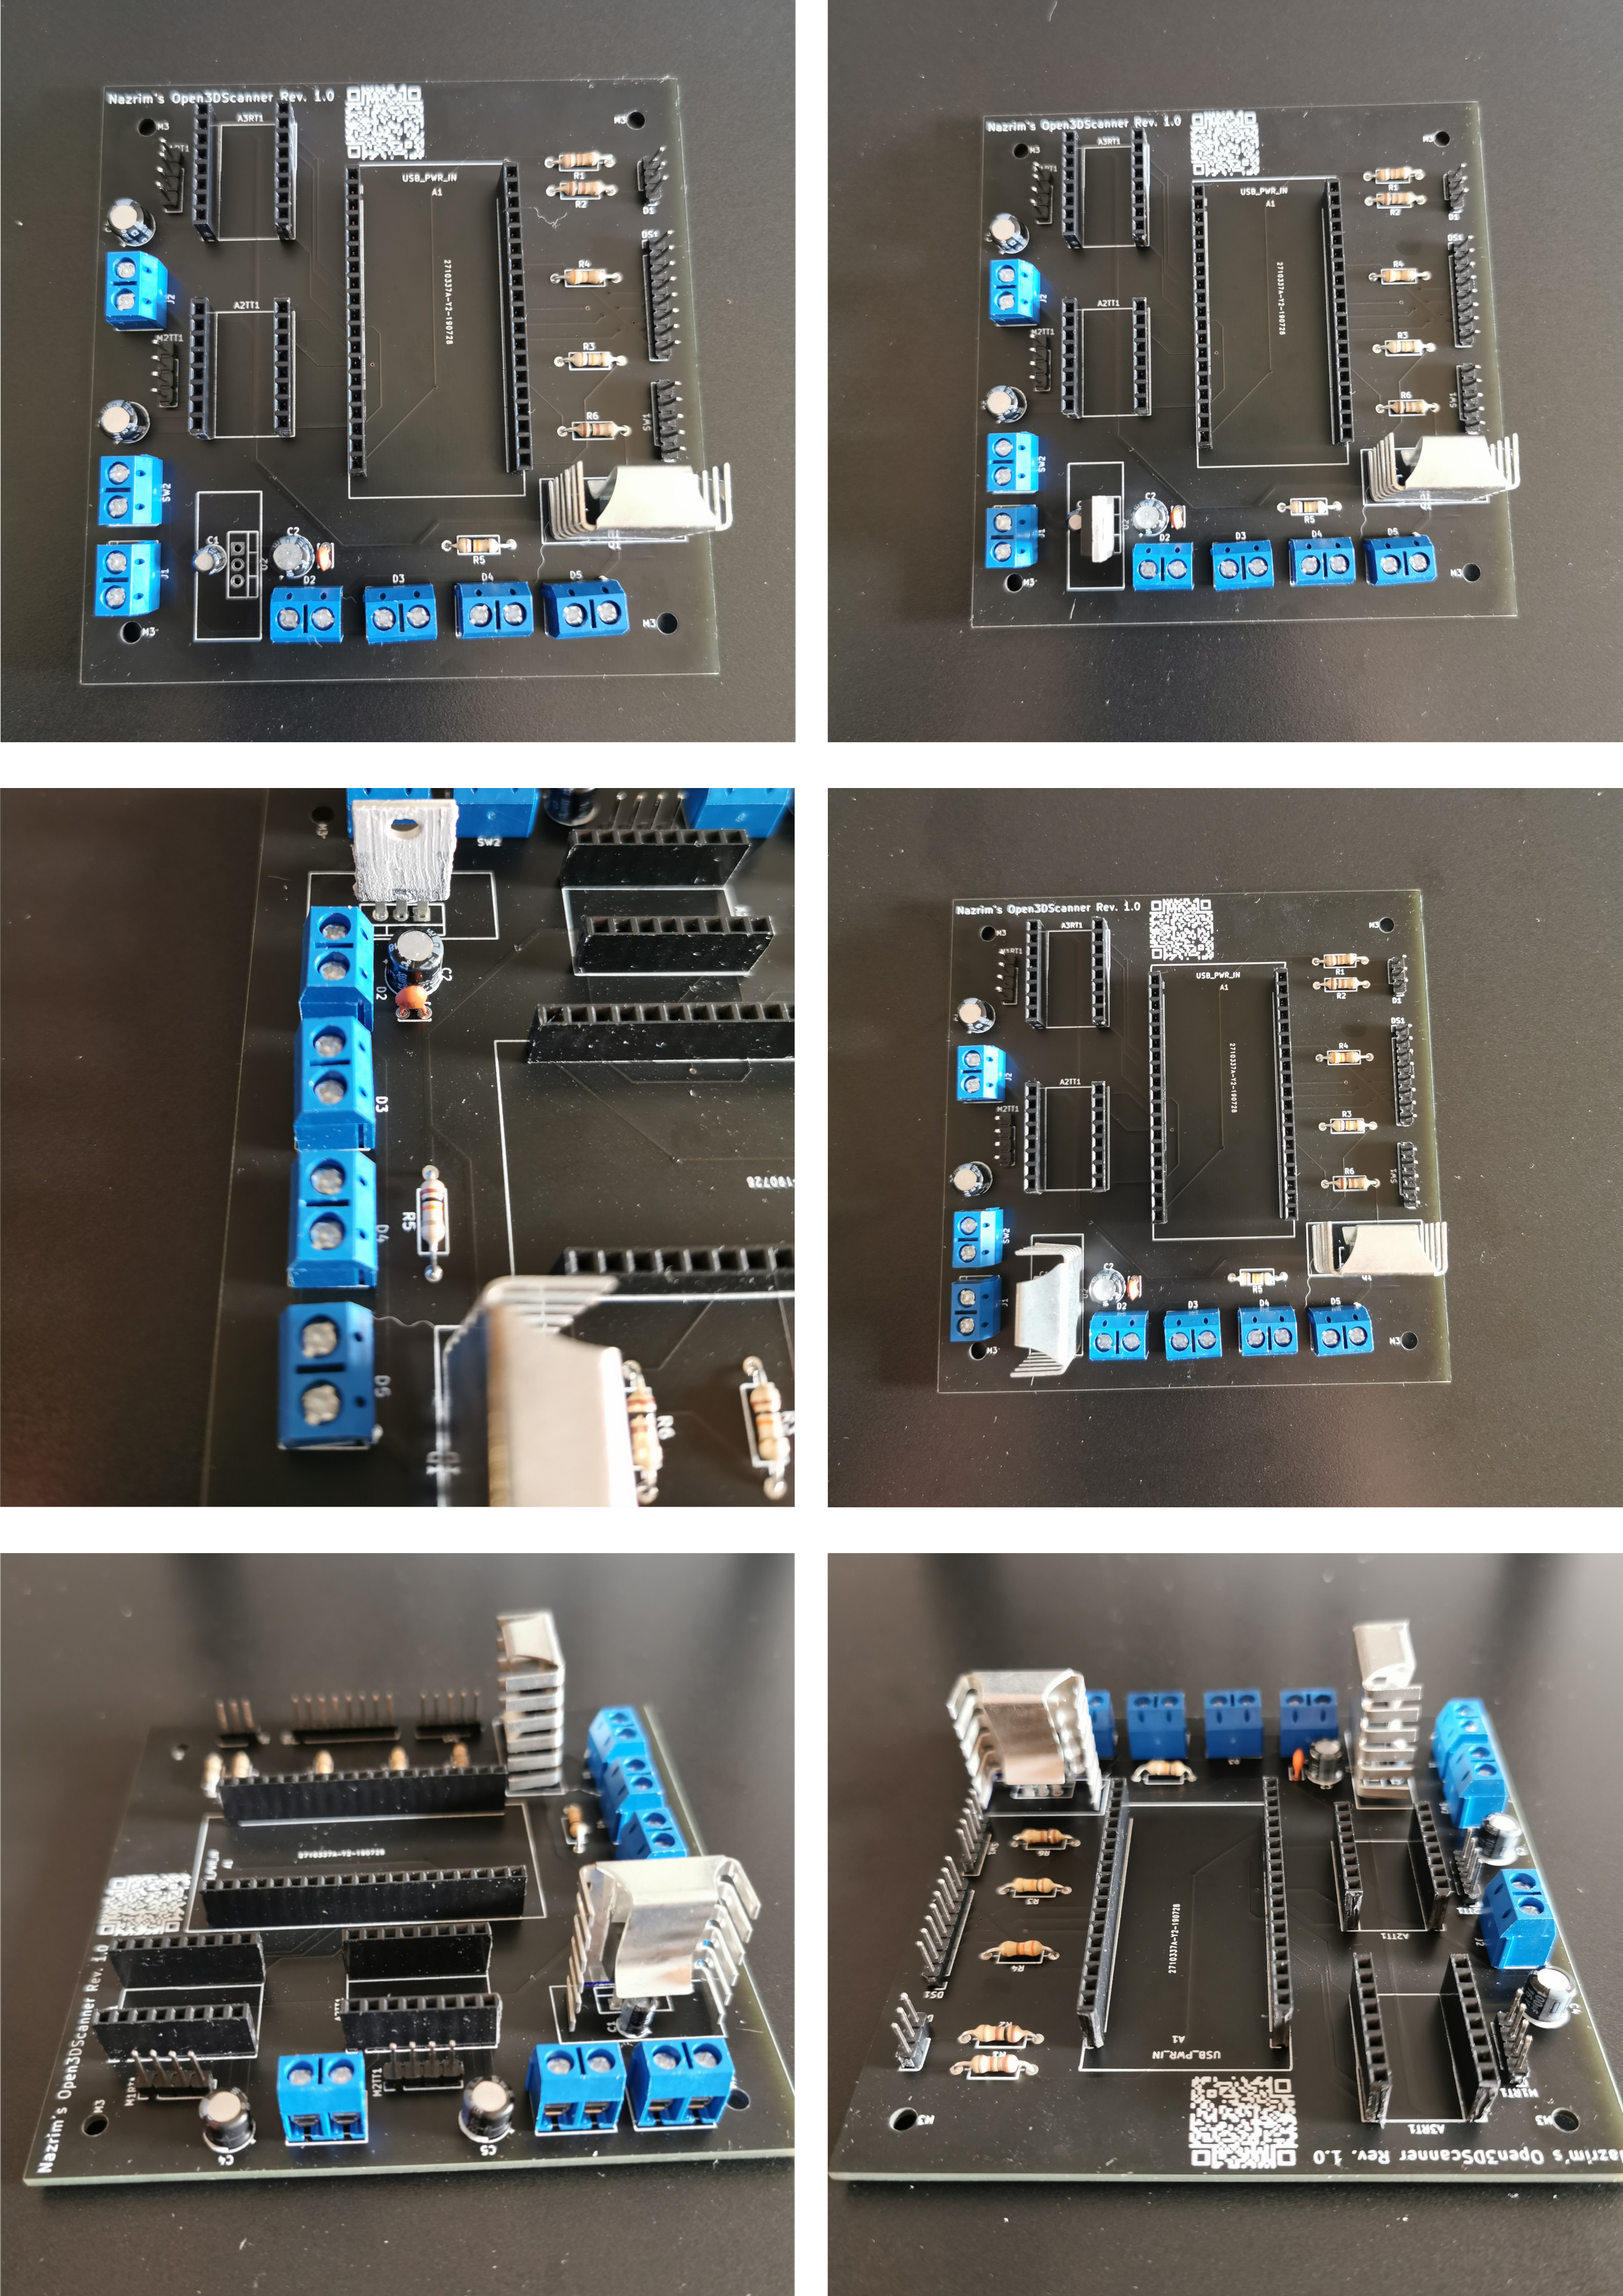
\includegraphics[width=\linewidth]{images/PcbSeries6.jpg}%
		\caption{Steps \numrange[text-rm=\lightBoldFont]{31}{36} of PCB assembly}%
	\end{centered}%
\end{figure}%

\begin{figure}[ht!]%
	\begin{centered}%
		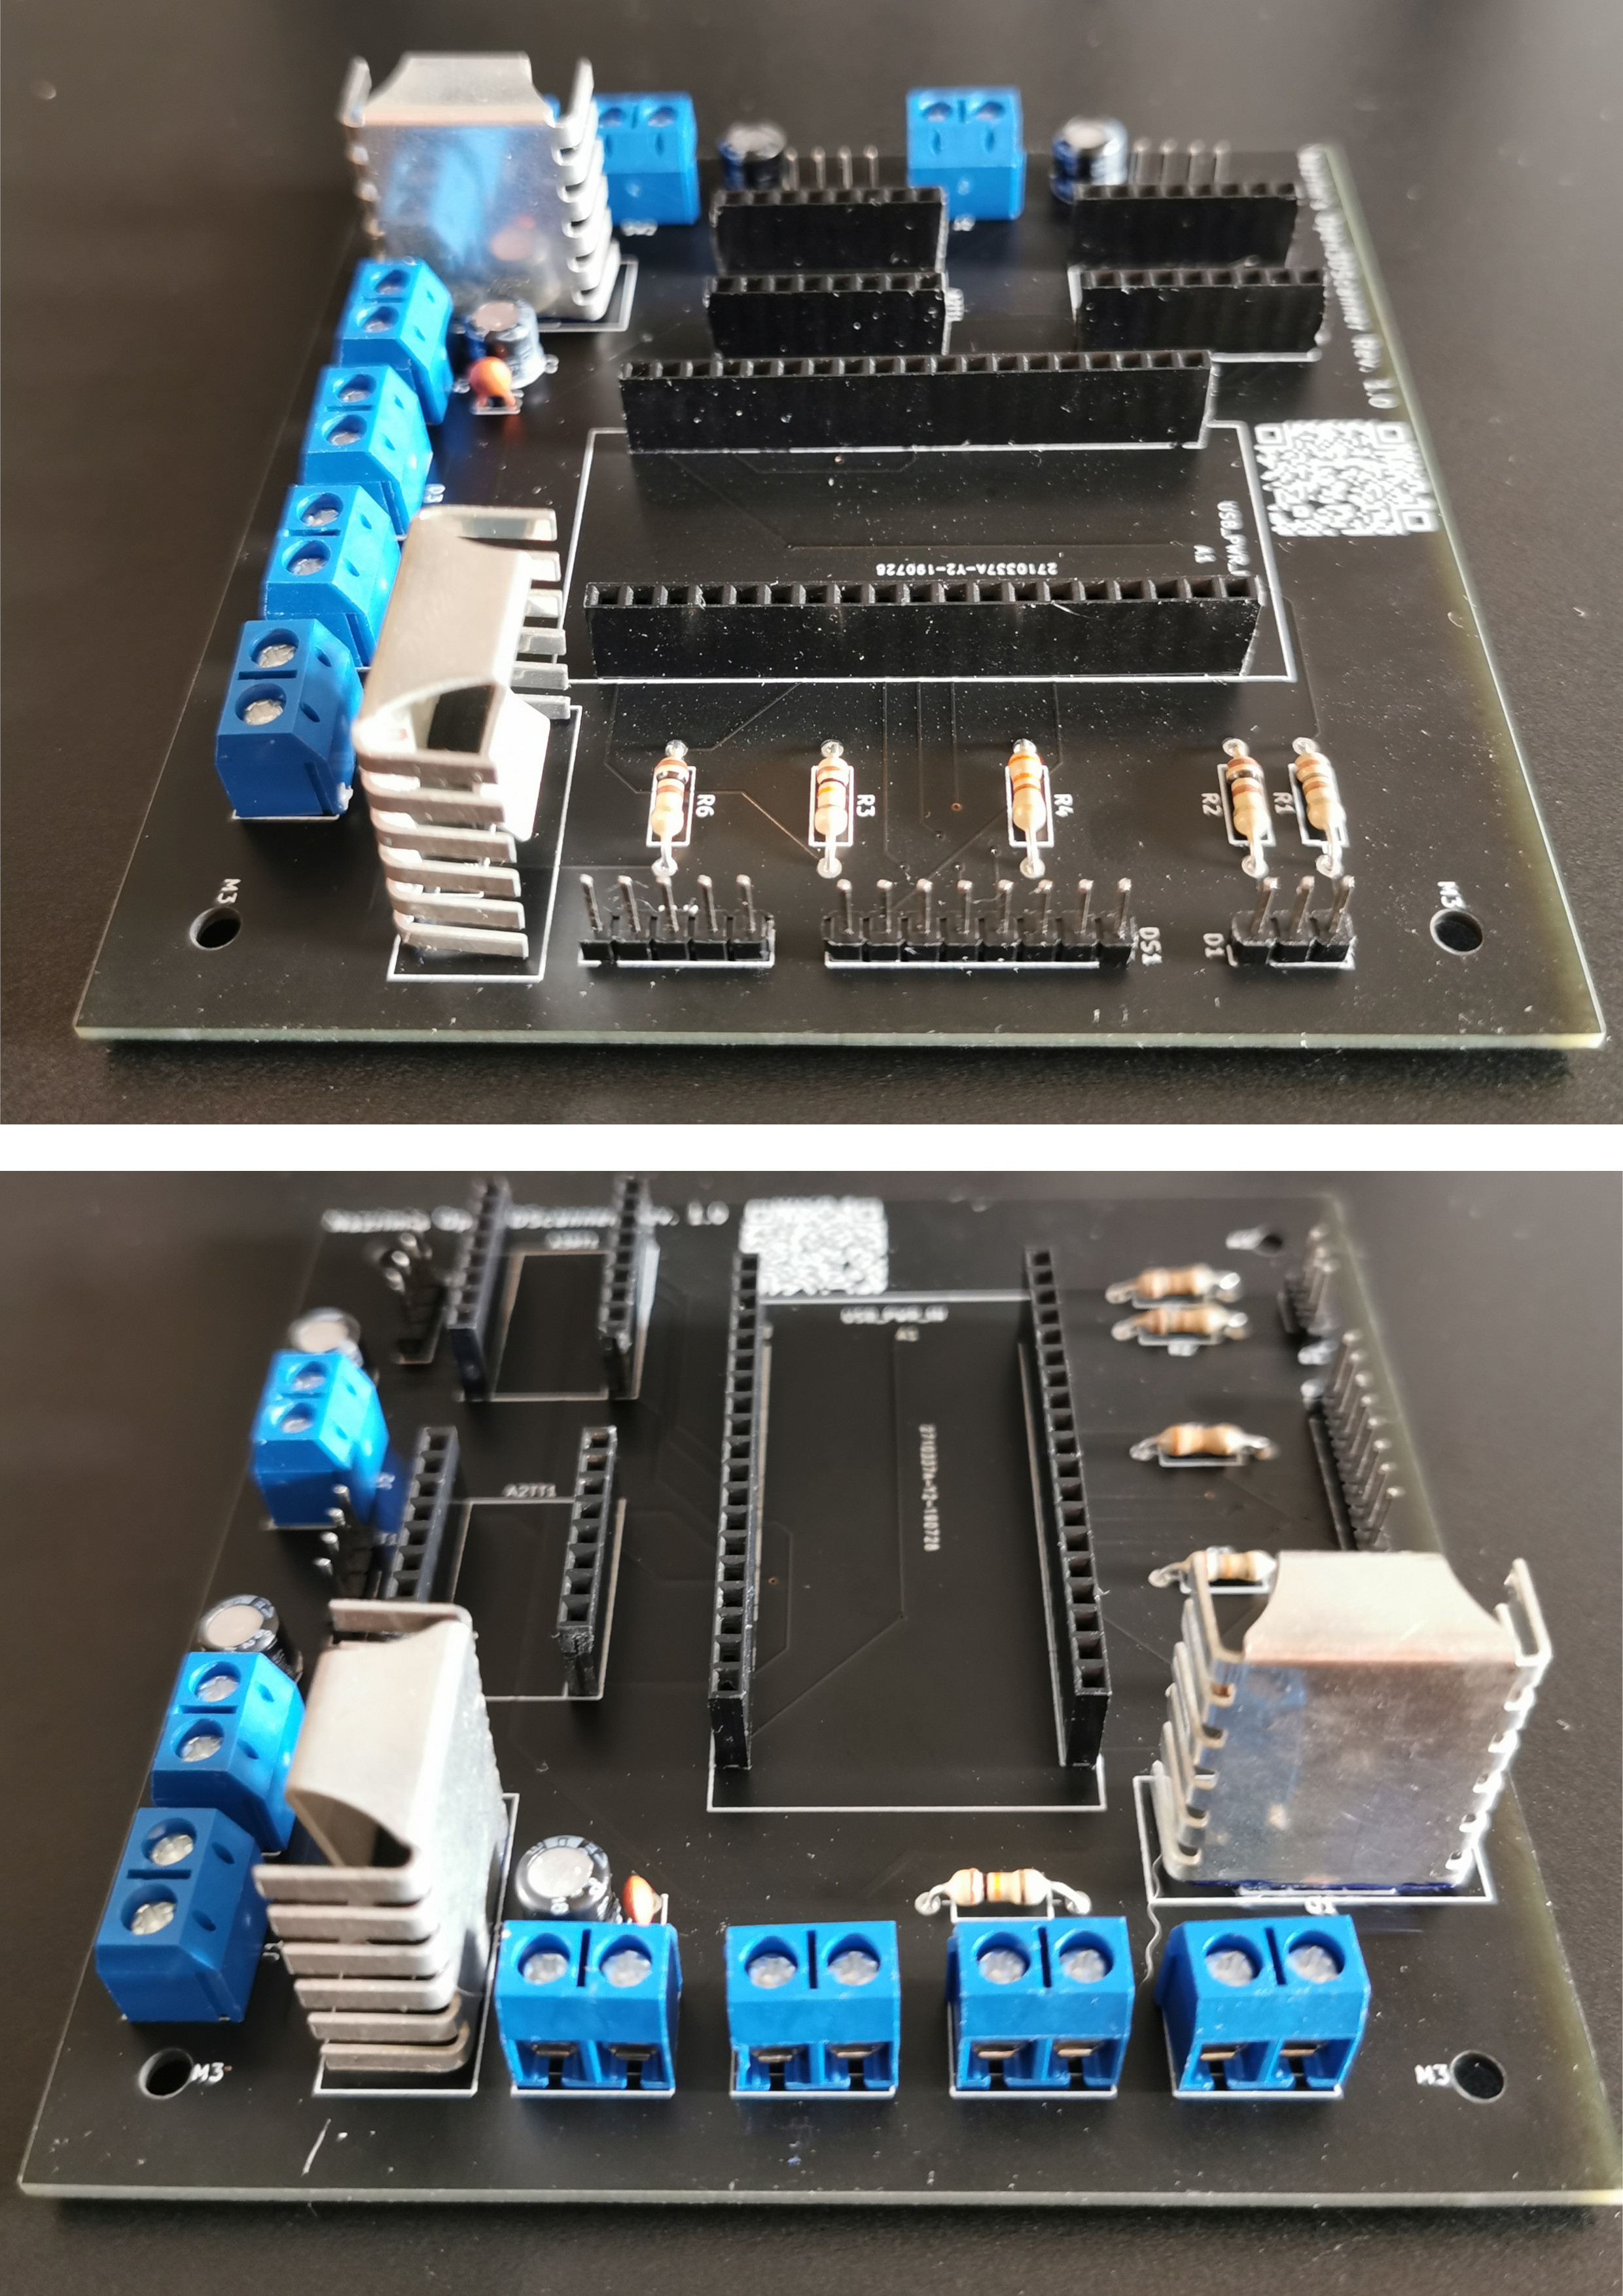
\includegraphics[width=\linewidth]{images/PcbSeries7.jpg}%
		\caption{Steps \numrange[text-rm=\lightBoldFont]{37}{38} of PCB assembly}%
	\end{centered}%
\end{figure}%
	\indexprologue{%
		\label{ca:refs}%
		In case the document is available in printed form, this chapter contains all used links, which are provided with alternative display texts. This also allows these references to be followed.%
		
		The references are sorted alphabetically and not according to their appearance in the document.A few of the link texts are interpreted as special characters (e.g. \hologo{XeLaTeX}), so they do not appear at the expected position of the index, but at the beginning.%
		
		All links listed in this appendix were checked for validity on \urlCheckedOne.%
	}%
	\printindex[hrefs]%
\end{document}%